% Beamer presentation of the Phantom_ZZ_N10 run:
%   Part 0 : Title and one-sentence roadmap
%   Part A : Model, field-dressed bulk, phantom helix, ZZ channel, generator, and witnesses
%   Part B : Reading guide: Gamma(t) dictionary, exact invariants, and numerical checks
%   Part C : Complete dynamical characterization (reduced edge state and quantum channel)
%   Part D : Synthesis around t = 222.60 and open questions
%   Appendix: Full 83-plot inventory, duplicate/companion thumbnails, and canonical-form derivation
% Build from reports/:
%   pdflatex -synctex=1 -interaction=nonstopmode -halt-on-error phantom_zz_n10_beamer.tex
%   bibtex phantom_zz_n10_beamer
%   pdflatex -synctex=1 -interaction=nonstopmode -halt-on-error phantom_zz_n10_beamer.tex
%   pdflatex -synctex=1 -interaction=nonstopmode -halt-on-error phantom_zz_n10_beamer.tex
\documentclass[aspectratio=169,11pt]{beamer}
\usepackage[T1]{fontenc}
\usepackage[utf8]{inputenc}
\usepackage{lmodern}
\usepackage{graphicx}
\graphicspath{{./}{Phantom_ZZ_N10/}{reports/}{reports/Phantom_ZZ_N10/}}
\usepackage{amsmath,amssymb,mathtools,booktabs,array}
\usepackage[numbers,sort&compress]{natbib}
\renewcommand{\bibsection}{}
\providecommand{\doi}[1]{\href{https://doi.org/#1}{\nolinkurl{doi:#1}}}

\definecolor{ink}{RGB}{25,43,60}
\definecolor{accent}{RGB}{0,110,125}
\definecolor{muted}{RGB}{95,110,125}
\setbeamercolor{normal text}{fg=ink,bg=white}
\setbeamercolor{structure}{fg=accent}
\setbeamercolor{frametitle}{fg=accent}
\setbeamertemplate{navigation symbols}{}
\setbeamertemplate{bibliography item}[text]
\setbeamertemplate{footline}[frame number]
\setbeamersize{text margin left=8mm,text margin right=8mm}
\setbeamertemplate{itemize item}{\small$\bullet$}

\newcommand{\ket}[1]{\lvert #1\rangle}
\newcommand{\bra}[1]{\langle #1\rvert}
\newcommand{\Tr}{\operatorname{Tr}}
\newcommand{\id}{\mathrm{id}}
\newcommand{\diag}{\operatorname{diag}}
\newcommand{\rank}{\operatorname{rank}}
\newcommand{\spec}{\operatorname{spec}}
\newcommand{\ZZ}{\mathrm{ZZ}}
\newcommand{\dmat}{\mathsf d}
\newcommand{\Heff}{H_{\mathrm{eff}}}
\newcommand{\St}{\mathsf S_t}
\newcommand{\Lt}{\mathsf L_t}
\newcommand{\mutednote}[1]{{\color{muted}\scriptsize #1}}

\title{Phantom-helix bulk, ZZ edge coupling:\\full dynamical characterization ($N = 10$)}
\subtitle{Complete reduced-state and quantum-channel analysis of the \texttt{Phantom\_ZZ\_N10} run}
\author{Spin transport project}
\date{20 November 2026}

\begin{document}

% ==============================================================
% Part 0 --- Opening
% ==============================================================

\begin{frame}[plain]
\titlepage
\end{frame}

\begin{frame}{Outline and central message}
\small
\begin{enumerate}\setlength\itemsep{5pt}
\item \textbf{Part A --- Model, notation, and witnesses:} field-dressed XXZ bulk, $\ket{\Psi_1^+}$ helix, $\ZZ$ Schur channel, canonical generator, and RHP / BLP diagnostics.
\item \textbf{Part B --- Reading guide:} exact $\Gamma(t)$ dictionary, conserved $z$-sector constants, and machine-precision consistency checks across all $83$ exported plots.
\item \textbf{Part C --- Dynamical results:} overlaps $\Gamma_{ab}(t)$, symmetries, coherences, entropies, correlations, entanglement, Choi spectrum, conditioning, rates, and non-Markovianity.
\item \textbf{Part D --- Synthesis:} zoom on the near-zero at $t=222.60$ and open questions.
\end{enumerate}
\medskip
\begin{center}
\fbox{\parbox{0.93\textwidth}{\centering
\textbf{Central message:} With the $\ket{++}$ edge input, $\rho_{AB}(t)=\Gamma(t)/4$---every edge-state and channel observable is a smooth function of $\Gamma(t)$; \textbf{only inverse-based quantities ($\Lambda_t^{-1}$)} spike.}}
\end{center}
\end{frame}

% ==============================================================
\section{Part A: Model, notation, and witnesses}
% ==============================================================

\begin{frame}{System, basis, and spin conventions}
\small
\[
\mathcal H = \mathcal H_A \otimes \mathcal H_{M_1}\otimes\cdots\otimes\mathcal H_{M_N}\otimes\mathcal H_B,\qquad
N=10\text{ bulk spins},\quad L=N+2=12\text{ total spins}.
\]
\begin{itemize}\setlength\itemsep{5pt}
\item \textbf{Spin-$\tfrac12$ operators:} $S_j^\alpha = s_{A,B}^\alpha = \tfrac12\sigma^\alpha$ with $\hbar=1$, computational basis $\ket0=\ket\uparrow$, $\ket1=\ket\downarrow$, and ordered two-edge basis $\{\ket{00},\ket{01},\ket{10},\ket{11}\}$.
\item \textbf{Information units:} von Neumann entropies $S(\rho)=-\Tr(\rho\ln\rho)$ and mutual information are measured in \textbf{nats} ($\ln 2\approx 0.6931$, $\ln 4\approx 1.3863$).
\item \textbf{Plot-axis conventions:} local expectations and two-point correlators use Pauli matrices $\sigma^\alpha$ (not $S^\alpha$), and plot labels write $\sigma_1\equiv\sigma_A$, $\sigma_L\equiv\sigma_B$, and $\Phi_t\equiv\Lambda_t$.
\item \textbf{Exact propagation:} spectral diagonalization on $t\in[0,500]$, $\delta t=0.01$ ($50{,}001$ samples; no ODE time-stepping approximation).
\end{itemize}
\end{frame}

% ==============================================================
\begin{frame}{Field-dressed bulk Hamiltonian}
\small
\[
H_M = J\sum_{j=1}^{N-1}\bigl(S_j^xS_{j+1}^x + S_j^yS_{j+1}^y + \Delta\,S_j^zS_{j+1}^z\bigr)
+ \frac{J}{2}S_1^x + \frac{J}{2}\bigl(\cos\varphi\,S_N^x + \sin\varphi\,S_N^y\bigr),\quad \Delta=\cos\gamma .
\]
\begin{itemize}\setlength\itemsep{5pt}
\item \textbf{Run parameters:} $J=1$, helix pitch $\gamma=\pi/3 \implies \Delta=\tfrac12$, and \texttt{PMC} boundary angle $\varphi=(N-3)\gamma \equiv \pi/3 \pmod{2\pi}$.
\item \textbf{Active boundary fields:} the transverse fields $\mathbf h_1=(J/2,0,0)$ and $\mathbf h_N=\tfrac{J}{2}(\cos\varphi,\sin\varphi,0)$ act on bulk ends $M_1,M_N$ throughout the evolution; no external fields act on $A,B$.
\item \textbf{Role:} they stabilize the phantom helix as an exact eigenstate of the open bulk chain.
\item \textbf{Broken $M_z$ conservation:} $[H_M,\sum_{j=1}^N S_j^z]\neq 0$ (largest $\Delta M_z\neq 0$ matrix element is $0.25$), so bulk magnetization sectors mix dynamically (\texttt{MagnetizationConservedExactly = False}).
\end{itemize}
\end{frame}

% ==============================================================
\begin{frame}{Initial bulk state: the phantom helix $\ket{\Psi_1^+}$}
\small
\[
\ket{\psi_M}=\ket{\Psi_1^+} = \bigotimes_{j=1}^{N}\frac{\ket0 - e^{i(j-2)\gamma}\ket1}{\sqrt2}\qquad
\bigl(\text{verified against \texttt{UploadedPhantom} to fidelity }1\bigr).
\]
\begin{columns}[T,totalwidth=\textwidth]
\begin{column}{0.55\textwidth}
\footnotesize\setlength{\tabcolsep}{4pt}
\centering
\begin{tabular}{@{}ll@{}}
\toprule
Quantity & Value in run \\\midrule
Size / pitch / branch & $N=10$, $\gamma=\varphi=\pi/3$, \texttt{PMC} \\
Bulk eigenenergy $E_M$ & $\tfrac{7}{8}=0.875$ ($\tfrac{9}{8}-\tfrac{1}{8}-\tfrac{1}{8}$) \\
Level degeneracy $d$ & $8$ (gap to $Q$: $\Delta E=0.0020$) \\
Eigenstate residual & $\lVert(H_M-E_M)\ket{\psi_M}\rVert_2 = 3.3\times 10^{-16}$ \\
Eigenspace weight & $1.000000000000002$ \\\bottomrule
\end{tabular}
\end{column}
\begin{column}{0.42\textwidth}
\footnotesize
\begin{itemize}\setlength\itemsep{4pt}
\item Equatorial product state with chiral in-plane spin rotation of step $\gamma=\pi/3$ per site.
\item Populates all $11$ bulk $M_z$ slices with binomial weights $w_\mu = 2^{-N}\binom{N}{N/2-\mu}$.
\item Lives inside an $8$-fold degenerate eigenspace of $H_M$ before coupling to $A,B$.
\end{itemize}
\end{column}
\end{columns}
\end{frame}

% ==============================================================
\begin{frame}{ZZ edge coupling and conditional bulk Hamiltonians}
\small
\[
H = H_M + V_{\ZZ},\qquad V_{\ZZ}=g\bigl(s_A^z S_1^z + S_N^z s_B^z\bigr)\quad(g=0.1),\qquad
U_t = \sum_{a\in\{00,01,10,11\}} \ket a\bra a \otimes e^{-iH_a t}.
\]
\begin{columns}[T,totalwidth=\textwidth]
\begin{column}{0.50\textwidth}
\footnotesize
\[
\begin{array}{@{}c@{\quad}l@{}}
\toprule
\text{Edge }a=(s_A,s_B) & \text{Conditional } H_a = H_M + V_a \\\midrule
00\;(+\tfrac12,+\tfrac12) & H_M + \tfrac{g}{2}S_1^z + \tfrac{g}{2}S_N^z \\[2pt]
01\;(+\tfrac12,-\tfrac12) & H_M + \tfrac{g}{2}S_1^z - \tfrac{g}{2}S_N^z \\[2pt]
10\;(-\tfrac12,+\tfrac12) & H_M - \tfrac{g}{2}S_1^z + \tfrac{g}{2}S_N^z \\[2pt]
11\;(-\tfrac12,-\tfrac12) & H_M - \tfrac{g}{2}S_1^z - \tfrac{g}{2}S_N^z \\\bottomrule
\end{array}
\]
\end{column}
\begin{column}{0.47\textwidth}
\footnotesize
\begin{itemize}\setlength\itemsep{4pt}
\item \textbf{Conserved edge $z$-projections:} $[H,s_A^z]=[H,s_B^z]=0$, even though bulk $M_z$ is not conserved.
\item \textbf{Boundary perturbation scale:} $\lVert V_a\rVert = g/2 = 0.05$, with $V_{\bar a}=-V_a$ for opposite edge labels.
\item \textbf{Exact block reduction:} four $1024\times 1024$ Hermitian diagonalizations replace one $4096\times 4096$ problem.
\end{itemize}
\end{column}
\end{columns}
\end{frame}

% ==============================================================
\begin{frame}{Conditional bulk states and the dephasing matrix}
\small
\[
\ket{\phi_a(t)} = e^{-iH_a t}\ket{\psi_M},\qquad
\Gamma_{ab}(t) = \langle\phi_b(t)\vert\phi_a(t)\rangle,\qquad a,b\in\{00,01,10,11\}.
\]
\begin{itemize}\setlength\itemsep{5pt}
\item \textbf{Gram-matrix structure:} $\Gamma(t)$ is the $4\times 4$ Gram matrix of the four normalized conditional bulk states $\ket{\phi_a(t)}\in\mathbb C^{1024}$.
\item \textbf{Exact positivity and bounds:} $\Gamma(t)\succeq 0$ (Hermitian positive semidefinite), $\Gamma_{aa}(t)=1$, and $\lvert\Gamma_{ab}(t)\rvert\le 1$ for every $t$, with $\Gamma_{ab}(0)=1$.
\item \textbf{Physical meaning of $\lvert\Gamma_{ab}(t)\rvert$:} measures distinguishability of the bulk states conditioned on $a$ vs.\ $b$; $\Gamma_{ab}=0$ means orthogonal conditional bulk states (complete $a$--$b$ dephasing).
\item \textbf{Six off-diagonal pairs:} $(00,01)$, $(00,10)$, $(00,11)$, $(01,10)$, $(01,11)$, and $(10,11)$ carry all dynamics.
\end{itemize}
\end{frame}

% ==============================================================
\begin{frame}{Exact reduced channel, Choi matrix, and transfer matrix}
\small
\[
\Lambda_t(X)=\Gamma(t)\circ X,\quad
C_t=\sum_{a,b}\ket a\bra b_R\otimes\Lambda_t(\ket a\bra b),\quad
\St=\diag\bigl(\operatorname{vec}_{\mathrm{row}}\Gamma(t)\bigr).
\]
\begin{itemize}\setlength\itemsep{4pt}
\item \textbf{Universal CPTP property:} $\Lambda_t(X)=\Tr_M[U_t(X\otimes\ket{\psi_M}\bra{\psi_M})U_t^\dagger]$ is CPTP at all times ($\Tr C_t=4$, Choi state $\omega_t=C_t/4$, Kraus rank $=\rank C_t=\rank\Gamma(t)\le 4$).
\item \textbf{Row-vectorized transfer matrix $\St$:} acts as $\operatorname{vec}_{\mathrm{row}}[\Lambda_t(X)]=\St\operatorname{vec}_{\mathrm{row}}(X)$ ($16\times 16$ diagonal).
\item \textbf{Symmetry superoperators:} $\mathcal R=\mathrm{SWAP}\otimes\mathrm{SWAP}$ (edge swap $A\leftrightarrow B$), $\mathcal F=(\sigma^x\otimes\sigma^x)^{\otimes 2}$ (edge spin flip), and $\epsilon_{U(1)}(\St)=\max_{q_{ab}\neq q_{cd}}\lvert(\St)_{(ab),(cd)}\rvert$ ($z$-charge violation).
\item \textbf{Response matrices ($\rho_B=\ket1\bra1$):} $[M_{A\to Q}(t)]_{\alpha\beta}=\tfrac12\operatorname{Re}\Tr\bigl[\sigma_Q^\alpha\Tr_{\bar Q}\Lambda_t(\sigma_A^\beta\otimes\rho_B)\bigr]$ for $Q\in\{A,B\}$.
\end{itemize}
\end{frame}

% ==============================================================
\begin{frame}{With the $\ket{++}$ input, the reduced state is the channel}
\small
\[
\ket{\psi_{AB}(0)}=\ket{++}=\frac12\sum_a\ket a,\qquad
\rho_{AB}(0)=\frac14\,\mathbf1\mathbf1^{\mathsf T}
\quad\Longrightarrow\quad
\boxed{\rho_{AB}(t)=\Lambda_t\bigl(\rho_{AB}(0)\bigr)=\frac14\,\Gamma(t).}
\]
\begin{itemize}\setlength\itemsep{5pt}
\item \textbf{State--Choi coincidence:} the Choi state $C_t/4$ embeds $\Gamma(t)/4$ on rows and columns $\{1,6,11,16\}$ with $12$ structural zeros elsewhere, so $\spec(C_t/4)=\spec(\rho_{AB}(t))\cup\{0^{\times 12}\}$.
\item \textbf{Maximal coherence probe:} starting with $\rho_{ab}(0)=1/4$ for every pair $(a,b)$ exposes all six off-diagonal factors $\Gamma_{ab}(t)$ directly as $4\,\rho_{AB;ab}(t)$.
\item \textbf{Redundancy across exports:} nearly $40\%$ of the $83$ exported \texttt{State\_*} and \texttt{Channel\_*} plots become exact rescalings or algebraic functions of one another (summarized in Part~B).
\end{itemize}
\end{frame}

% ==============================================================
\begin{frame}{Time-local generator and conditioning}
\small
\[
\dot\rho_{AB}=\mathcal L_t(\rho_{AB}),\quad
\Lt = \dot{\mathsf S}_t\,\St^{-1} = \diag\bigl(\operatorname{vec}_{\mathrm{row}}[\dot\Gamma\oslash\Gamma]\bigr),\quad
\eta_{ab}(t)=\frac{\dot\Gamma_{ab}(t)}{\Gamma_{ab}(t)}=-\kappa_{ab}(t)+i\omega_{ab}(t).
\]
\begin{itemize}\setlength\itemsep{5pt}
\item \textbf{Invertibility condition:} $\Lambda_t^{-1}$ exists iff $\sigma_{\min}(\St)=\min_{a<b}\lvert\Gamma_{ab}(t)\rvert>0$; the code evaluates $\Lt$ whenever $\sigma_{\min}(\St)\ge 10^{-8}$ (\texttt{MinimumSingularValue}).
\item \textbf{Analytic numerator:} $\dot\Gamma_{ab}(t)$ is computed spectrally from $\ket{\dot\phi_a(t)}=-iH_a\ket{\phi_a(t)}$ (no finite differences), and obeys $\lvert\dot\Gamma_{ab}(t)\rvert\le\lVert V_a-V_b\rVert\le g = 0.1$.
\item \textbf{Conditioning amplification:} $\kappa_{ab}=-\tfrac{d}{dt}\ln\lvert\Gamma_{ab}\rvert$ and $\omega_{ab}=\tfrac{d}{dt}\arg\Gamma_{ab}$ divide by $\Gamma_{ab}(t)$, turning any near-zero of $\lvert\Gamma_{ab}\rvert$ into a tall finite spike of $\Lt$.
\end{itemize}
\end{frame}

% ==============================================================
\begin{frame}{Canonical master equation and sorted rates}
\small
\[
\dmat(t)=G^{\mathsf T}\eta(t)\,G\quad\text{on }\{F_\mu\}=\Bigl\{\tfrac12\sigma_A^z\otimes I,\;\tfrac12 I\otimes\sigma_B^z,\;\tfrac12\sigma_A^z\otimes\sigma_B^z\Bigr\},\qquad
\bigl\{\tilde\gamma_1,\tilde\gamma_2,\tilde\gamma_3\bigr\}=\spec\dmat(t).
\]
\begin{itemize}\setlength\itemsep{4pt}
\item \textbf{Unique canonical form \cite{Hall2014}:} diagonal covariance and frozen populations restrict the $15\times 15$ GKS--Lindblad matrix to the $3\times 3$ Hermitian block $\dmat(t)$, plus diagonal $\Heff(t)$ (Appendix~3).
\item \textbf{Fifteen exported rates:} $\{\tilde\gamma_1,\tilde\gamma_2,\tilde\gamma_3\}$ are padded with $12$ structural zeros and sorted ascending at each $t$ into $\gamma_1(t)\le\cdots\le\gamma_{15}(t)$.
\item \textbf{Sorting caveat:} because sorting is repeated at every $t$, an index $\gamma_k(t)$ does not follow a fixed eigenoperator through eigenvalue crossings.
\item \textbf{Bounds and CP-divisibility:} $\gamma_1(t)\le\kappa_{ab}(t)\le\gamma_{15}(t)$ and $\lvert\gamma_k(t)\rvert\le\lVert\eta(t)\rVert_2$; $\gamma_1(t)<0$ signals local non-CP-divisibility while $\Lambda_t$ remains CPTP.
\end{itemize}
\end{frame}

% ==============================================================
\begin{frame}{Non-Markovianity witnesses (I): RHP CP-divisibility}
\small
\[
g_{\mathrm{RHP}}(t)=\frac12\sum_{k=1}^{15}\max\bigl(0,-\gamma_k(t)\bigr),\qquad
w_k=\max\!\left(0,\frac{\lVert C[\Lambda_{t_k}\Lambda_{t_{k-1}}^{-1}]\rVert_1}{4}-1\right),\quad
r_k=\frac{w_k}{\delta t}.
\]
\begin{itemize}\setlength\itemsep{5pt}
\item \textbf{Two-step propagator in $\ZZ$:} $\Phi_{t_k,t_{k-1}}=\Lambda_{t_k}\Lambda_{t_{k-1}}^{-1}$ is Schur multiplication by $Q_k=\Gamma(t_k)\oslash\Gamma(t_{k-1})$, evaluated directly on $4\times 4$ matrices when $\sigma_{\min}(\mathsf S_{t_{k-1}})\ge 10^{-8}$.
\item \textbf{Physical meaning:} $g_{\mathrm{RHP}}(t)>0$ (Rivas--Huelga--Plenio) quantifies the instantaneous rate at which intermediate maps fail complete positivity.
\item \textbf{Small-step consistency:} at uniform spacing $\delta t=0.01$ away from exact poles, $r_k=w_k/\delta t\to g_{\mathrm{RHP}}(t_k)$; both rely explicitly on $\Lambda_t^{-1}$.
\end{itemize}
\end{frame}

% ==============================================================
\begin{frame}{Non-Markovianity witnesses (II): selected-pair BLP backflow}
\small
\[
D(t)=\frac12\bigl\lVert\Lambda_t(\rho_1-\rho_2)\bigr\rVert_1,\qquad
\mathcal N(t_k)=\sum_{j=2}^{k}\max\bigl(0,D(t_j)-D(t_{j-1})\bigr).
\]
\begin{itemize}\setlength\itemsep{5pt}
\item \textbf{Selected orthogonal probe pair:} $\rho_1=\ket{++}\bra{++}$ and $\rho_2=\ket{+-}\bra{+-}$ give $\rho_1-\rho_2=\ket+\bra+_A\otimes\sigma_B^x$, so $D(0)=1$ and $\Lambda_t(\rho_1-\rho_2)$ probes $(00,01)$, $(00,11)$, $(01,10)$, $(10,11)$.
\item \textbf{No channel inversion:} $D(t)$ is linear in $\Gamma(t)$ (norm of a $4\times 4$ Hermitian matrix), so it stays smooth even if a $\Gamma_{ab}$ approaches zero.
\item \textbf{Interpretation:} $\dot D(t)>0$ (Breuer--Laine--Piilo) witnesses operational information backflow from the bulk to the edges (a lower bound on pair-optimized BLP).
\end{itemize}
\end{frame}

% ==============================================================
\section{Part B: Reading guide}
% ==============================================================

\begin{frame}{Dictionary: edge-state and channel plots from $\Gamma(t)$}
\footnotesize
Verified numerically across all $50{,}001$ samples to $<4\times 10^{-12}$ (remaining duplicates in Appendix~1):
\smallskip
\begin{center}
\scriptsize\setlength{\tabcolsep}{4pt}
\begin{tabular}{@{}lll@{}}
\toprule
Exported plot(s) & Exact formula in terms of $\Gamma(t)$ & Consequence \\\midrule
\texttt{State\_EdgeCoherences\_*} & $\Gamma_{ab}(t)/4\quad(a<b)$ & $1/4\times$\texttt{Channel\_Gamma\_*} \\
\texttt{Channel\_MapEntropy} & $S\bigl(\Gamma(t)/4\bigr)$ & $\equiv$ \texttt{State\_EntropyAB} \\
\texttt{Channel\_EntanglingConcurrence} & $C\bigl[\Gamma(t)/4\bigr]$ & $\equiv$ \texttt{State\_Concurrence} \\
\texttt{Channel\_ChoiEigenvalues} & $\spec\Gamma(t)\cup\{0^{\times 12}\}$ & $4\times$\texttt{State\_EdgeDensityEigenvalues} \\
\texttt{Channel\_MinSingularValue} & $\min_{a<b}\lvert\Gamma_{ab}(t)\rvert$ & Conditioning of $\Lambda_t^{-1}$ \\
\texttt{Channel\_ChoiNegativity} & $\tfrac14\sum_{a<b}\lvert\Gamma_{ab}(t)\rvert$ & $\tfrac12\,\ell_1$-coherence ($1.5$ at $t=0$) \\
\texttt{State\_LocalAX}, \texttt{LocalAY} & $\tfrac12\operatorname{Re},\,-\tfrac12\operatorname{Im}(\Gamma_{00,10}+\Gamma_{01,11})$ & $\langle\sigma_B^x\rangle=\langle\sigma_A^x\rangle,\;\langle\sigma_B^y\rangle=-\langle\sigma_A^y\rangle$ \\
\texttt{State\_Purity} & $\bigl(4+2\sum_{a<b}\lvert\Gamma_{ab}(t)\rvert^2\bigr)/16$ & Frobenius norm of $\Gamma/4$ \\\bottomrule
\end{tabular}
\end{center}
\smallskip
\mutednote{\textbf{Sole exception:} \texttt{State\_FullOverlap} probes the global $ABE$ ket via $\langle\psi_M\vert\phi_a(t)\rangle$ rather than $\Gamma_{ab}=\langle\phi_b\vert\phi_a\rangle$ (Slide~C10).}
\end{frame}

% ==============================================================
\begin{frame}{What is exactly constant, and why}
\footnotesize
Because $[H,s_A^z]=[H,s_B^z]=0$ and $\Lambda_t(X)=\Gamma(t)\circ X$ with $\Gamma_{aa}(t)=1$, $15$ exported plots are structurally trivial:
\smallskip
\begin{center}
\scriptsize\setlength{\tabcolsep}{3pt}
\begin{tabular}{@{}lll@{}}
\toprule
Omitted PNG(s) & Exact value & One-line reason \\\midrule
\texttt{State\_EdgePopulations} & $1/4$ each & Diagonal entries $\rho_{aa}(t)=\rho_{aa}(0)$ frozen \\
\texttt{State\_MagnetizationA/B}, \texttt{LocalAZ/BZ} & $0$ & Frozen populations ($1/4+1/4-1/4-1/4$) \\
\texttt{State\_CorrelationZZ}, \texttt{ConnectedZZ} & $0$ & Frozen populations \\
\texttt{State\_CurrentLeft}, \texttt{CurrentRight} & $0$ & $[H,s_A^z]=[H,s_B^z]=0$ \\
\texttt{Channel\_SignalAtoB} & $0$ & Probe $\rho_B=\ket1\bra1$ samples only $\Gamma_{aa}=1$ \\
\texttt{Channel\_RetentionA} & $1$ & $\sigma_A^z$ conserved ($\sigma_{\max}(M_{A\to A})=1$) \\
\texttt{Channel\_UnitalityError}, \texttt{MixedInputEntropy} & $0$, $\;\ln 4$ & Unital Schur map: $\Lambda_t(I_4/4)=I_4/4$ \\
\texttt{Channel\_U1CovarianceError}, \texttt{DephasingPop.\,Err.} & $0$, $\;0$ & Diagonal $\St$ and $\Gamma_{aa}=1$ \\
\texttt{Channel\_KrausRank} & $4$ ($t\ge 0.13$) & $1$ at $t=0$; $3$ on $[0.01,0.12]$ ($10^{-10}$ tol.) \\\bottomrule
\end{tabular}
\end{center}
\smallskip
\mutednote{All $15$ PNGs above are present in \texttt{Phantom\_ZZ\_N10/} and catalogued in Appendix~1, but omitted from Part~C.}
\end{frame}

% ==============================================================
\begin{frame}{Numerical-consistency checks}
\footnotesize
The exported error PNGs use Mathematica's default $[-1,1]$ axis (after $10^{-12}$ record chopping), showing only flat zeros. Their actual raw pre-chop extrema over all $50{,}001$ samples are at machine precision:
\smallskip
\begin{center}
\begin{tabular}{@{}llll@{}}
\toprule
Diagnostic PNG & Quantity & Raw extremum (\texttt{Checks}) & Post-chop \\\midrule
\texttt{State\_TraceError} & $\max_t\lvert\Tr\rho_{AB}(t)-1\rvert$ & $7.11\times 10^{-15}$ & $0$ \\
\texttt{State\_HermiticityError} & $\max_t\lVert\rho_{AB}-\rho_{AB}^\dagger\rVert_F$ & $<10^{-12}$ & $0$ \\
(in \texttt{Checks}) & $\min_t\lambda_{\min}(\rho_{AB}(t))$ & $-8.36\times 10^{-16}$ & $0$ \\
\texttt{Channel\_TPError} & $\max_t\lVert\Tr_{\mathrm{out}}C_t-I_4\rVert_{\max}$ & $4.57\times 10^{-14}$ & $0$ \\
\texttt{Channel\_ChoiTraceError} & $\max_t\lvert\Tr C_t-4\rvert$ & $2.84\times 10^{-14}$ & $0$ \\
\texttt{Channel\_MinChoiEigenvalue} & $\min_t\lambda_{\min}(C_t)$ & $-3.34\times 10^{-15}$ & $0$ \\
(in \texttt{Checks}) & $\max_t\lVert\Lambda_t(\rho_0)-\rho_{AB}(t)\rVert_{\max}$ & $0$ & $0$ \\\bottomrule
\end{tabular}
\end{center}
\smallskip
\mutednote{Master--worker parallel verification error across $12$ kernels ($1{,}563$ batches of $32$ samples): $0.0$.}
\end{frame}

% ==============================================================
\section{Part C: Dynamical characterization}
% ==============================================================

\begin{frame}{Conditional bulk overlaps $\lvert\Gamma_{ab}(t)\rvert$}
\begin{columns}[T,totalwidth=\textwidth]
\begin{column}{0.57\textwidth}
\centering
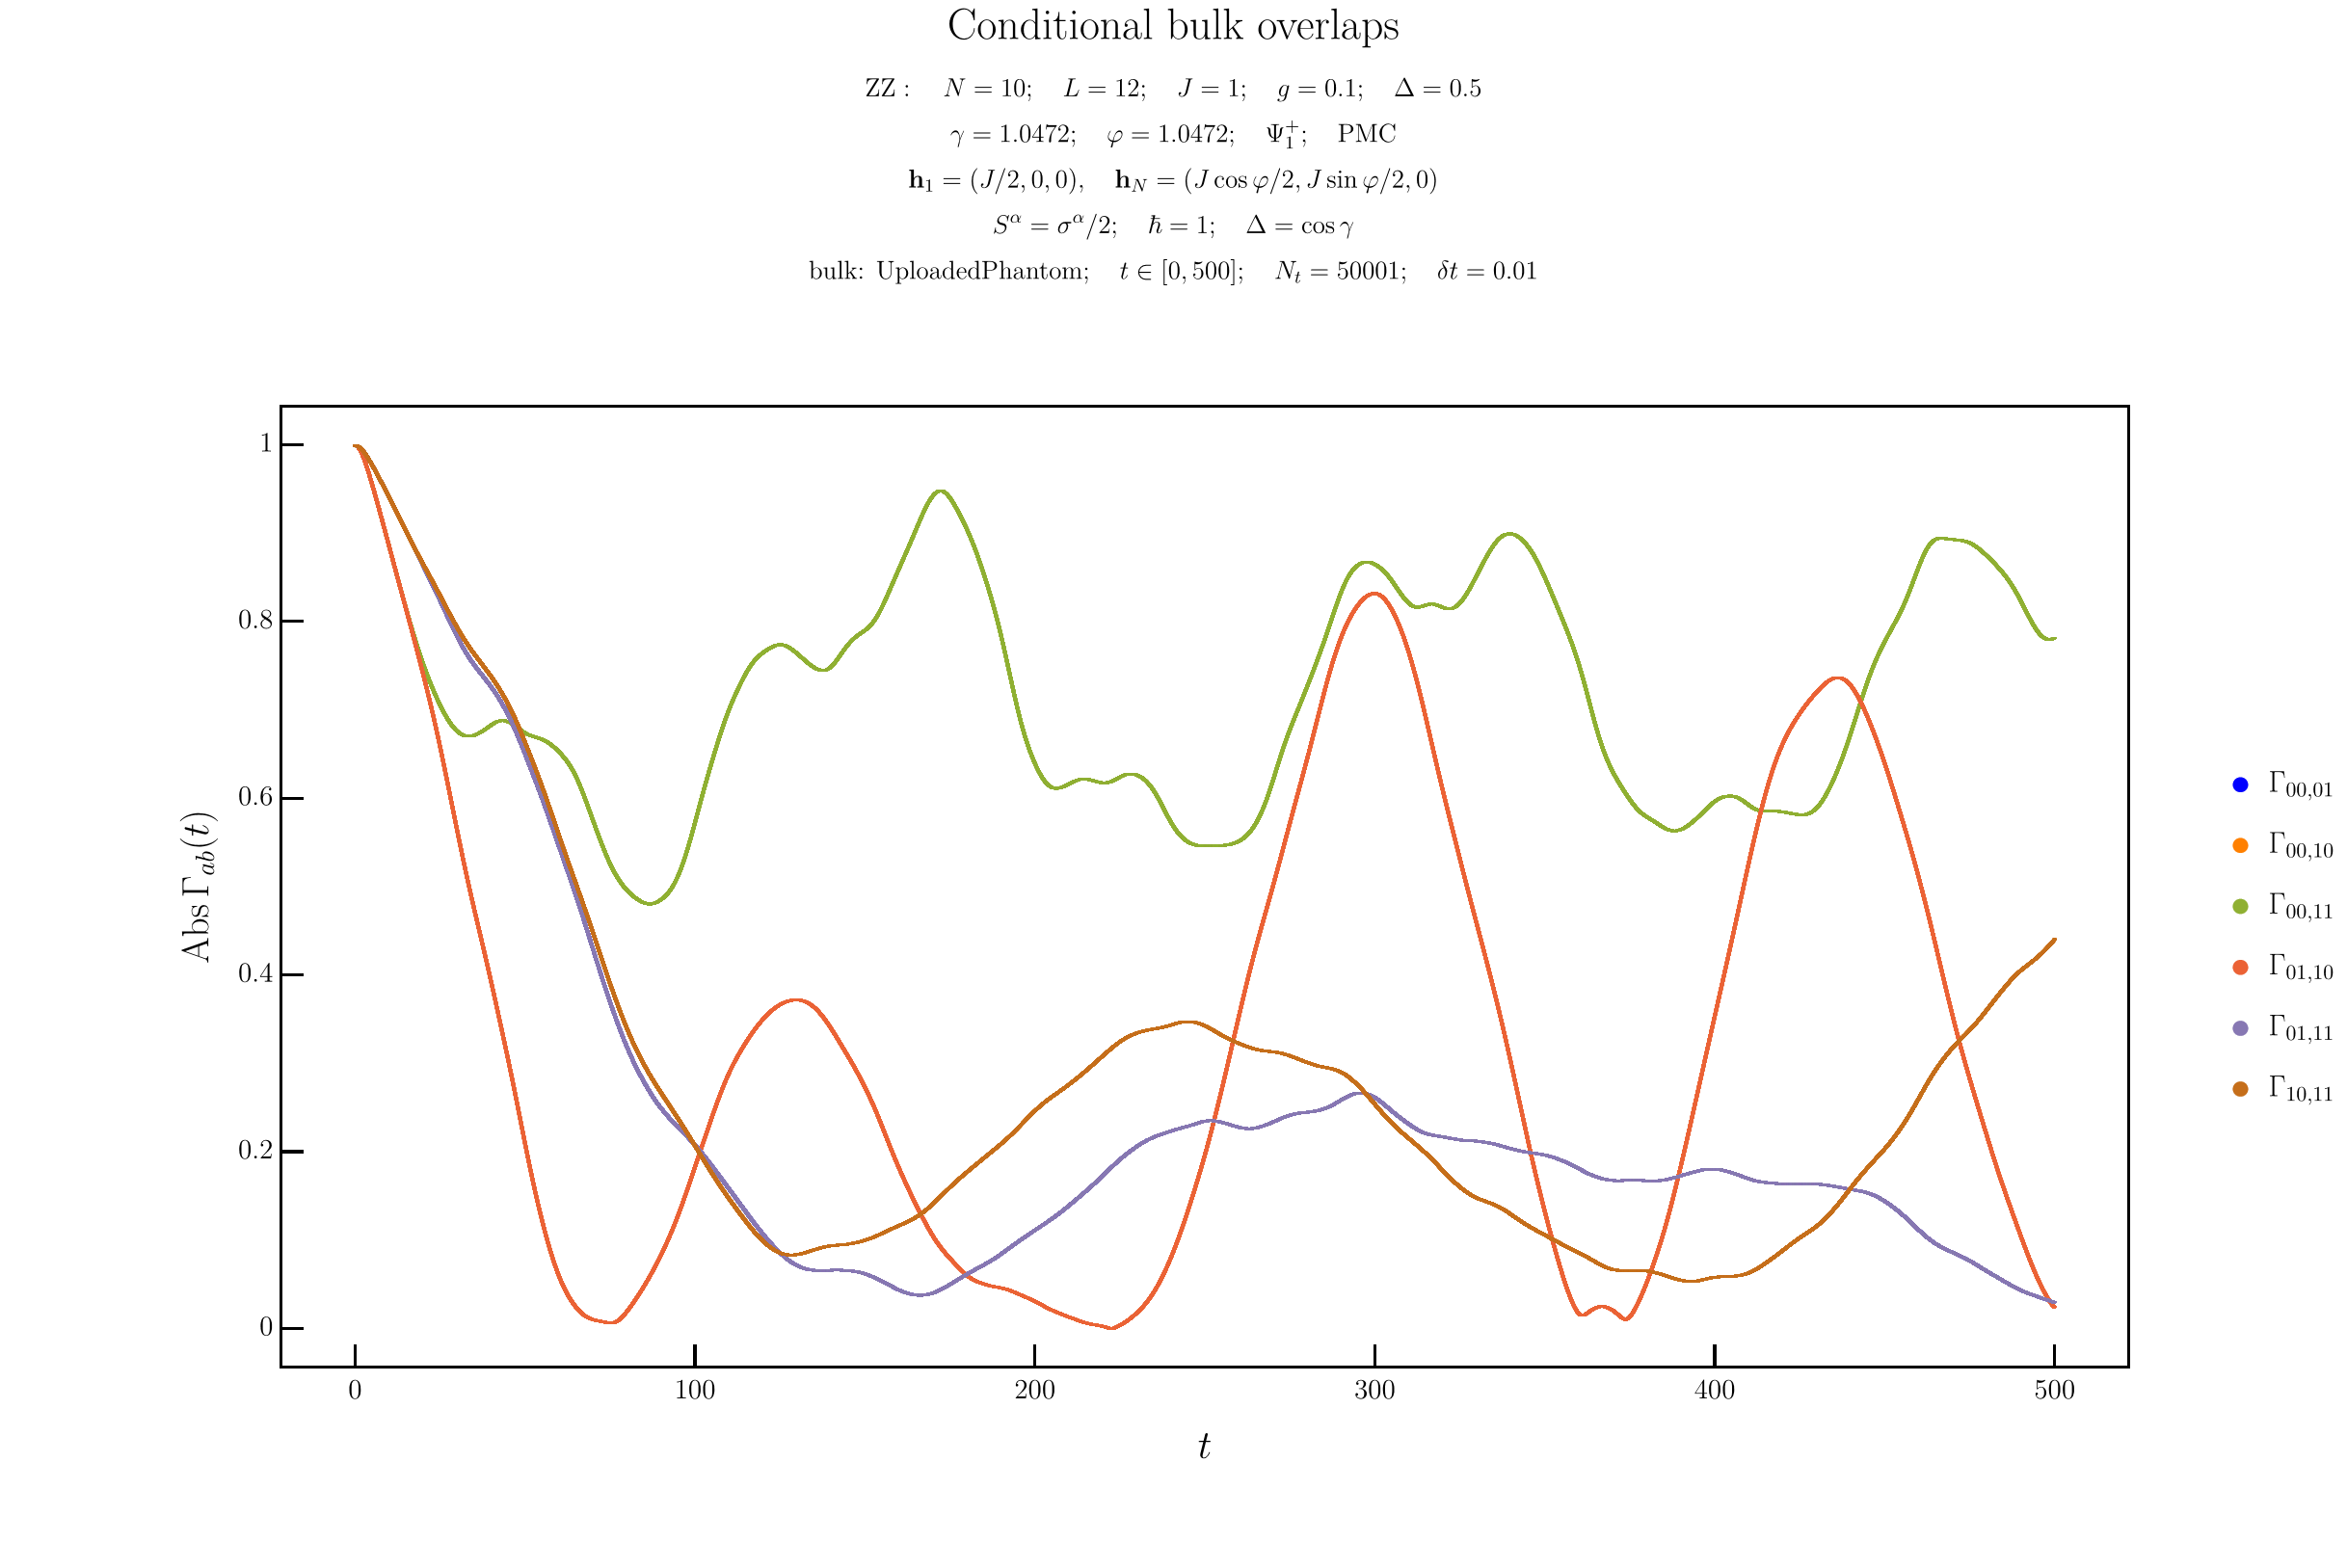
\includegraphics[width=\linewidth,height=0.77\textheight,keepaspectratio]{Phantom_ZZ_N10/Channel_Gamma_Abs.png}
\end{column}
\begin{column}{0.41\textwidth}
\footnotesize
\[
\lvert\Gamma_{ab}(t)\rvert=\bigl\lvert\langle\phi_b(t)\vert\phi_a(t)\rangle\bigr\rvert .
\]
\begin{itemize}\setlength\itemsep{4pt}
\item \textbf{Flip-flop $\Gamma_{01,10}$ (red):} explores $[0,1]$ most widely, with four near-zeros at $t=75.37$ ($6.7\times 10^{-3}$), $222.60$ ($1.07\times 10^{-4}$), $361.09$ ($1.5\times 10^{-2}$), and $373.80$ ($1.1\times 10^{-2}$).
\item \textbf{Double-quantum $\Gamma_{00,11}$ (green):} remains large throughout, in $[0.481,1]$ (reviving to $0.948$ at $t=172.3$).
\item \textbf{Two hidden curves:} $\lvert\Gamma_{00,01}\rvert$ and $\lvert\Gamma_{00,10}\rvert$ lie underneath $\lvert\Gamma_{01,11}\rvert$ (purple) and $\lvert\Gamma_{10,11}\rvert$ (brown) by $\mathcal R\mathcal F$ symmetry (Slide~C3).
\end{itemize}
\end{column}
\end{columns}
\end{frame}

% ==============================================================
\begin{frame}{Phases of $\Gamma(t)$: real and imaginary parts}
\footnotesize
\begin{columns}[T,totalwidth=\textwidth]
\begin{column}{0.49\textwidth}
\centering
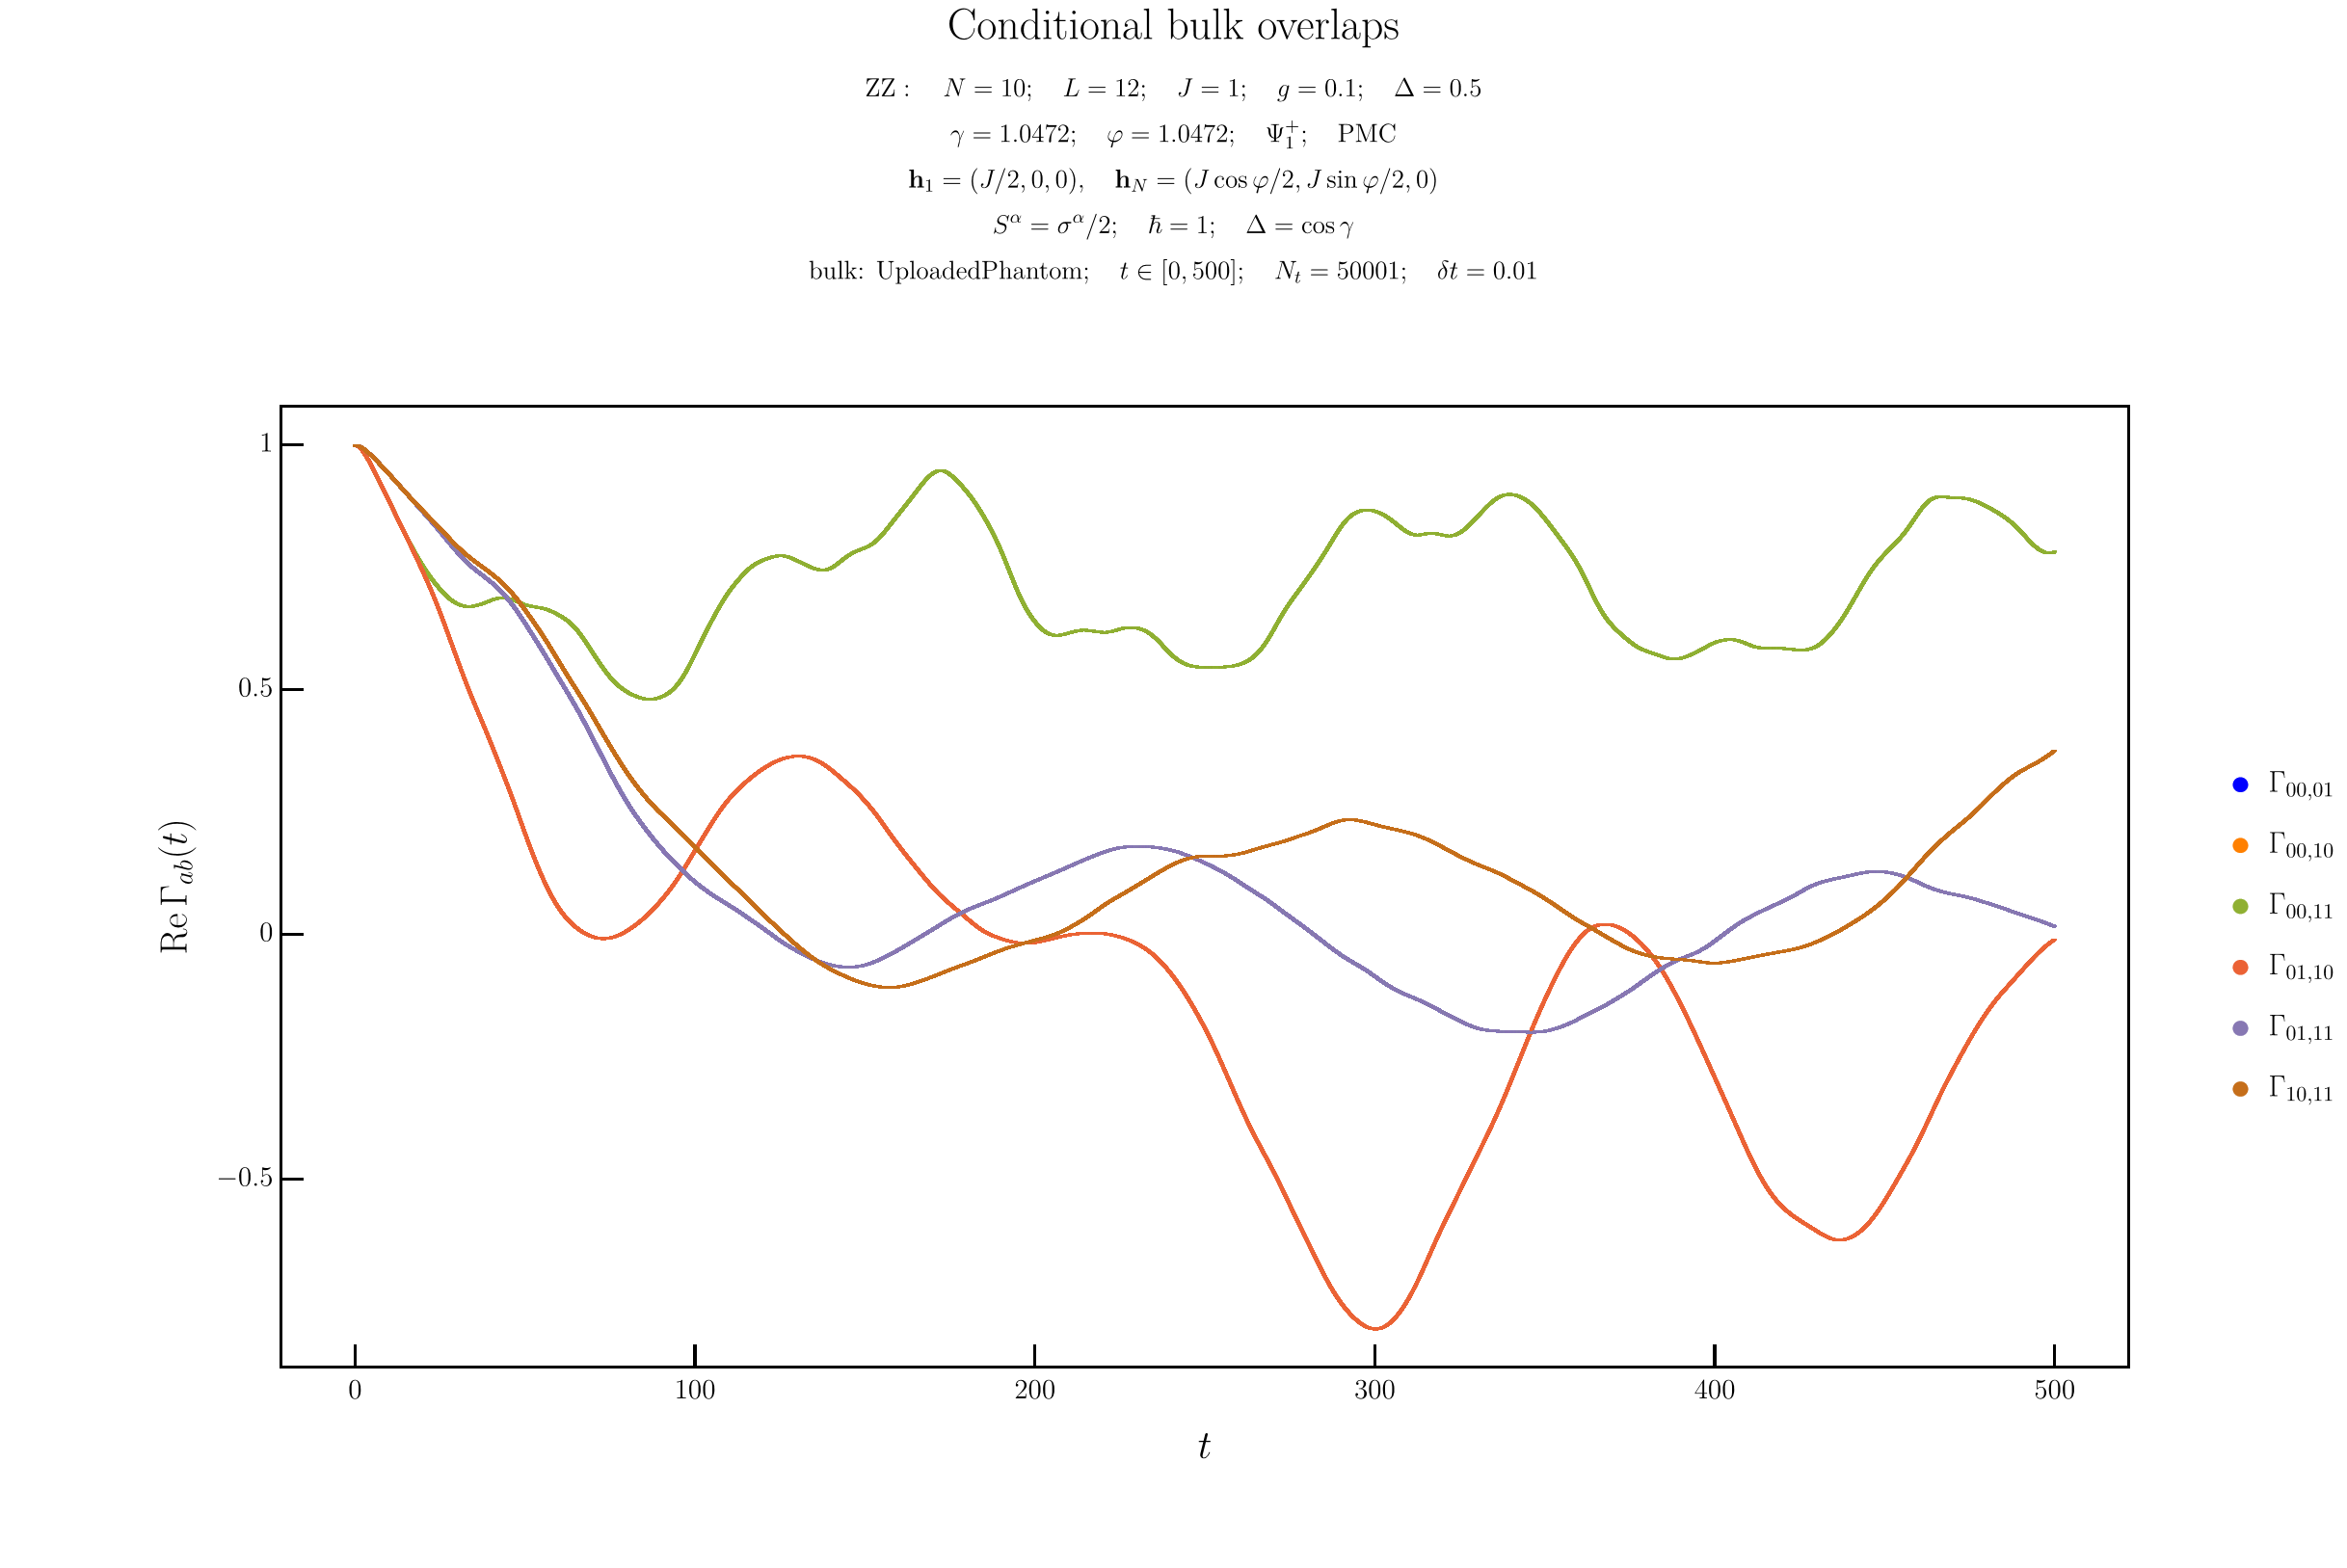
\includegraphics[width=\linewidth,height=0.50\textheight,keepaspectratio]{Phantom_ZZ_N10/Channel_Gamma_Re.png}
\end{column}
\begin{column}{0.49\textwidth}
\centering
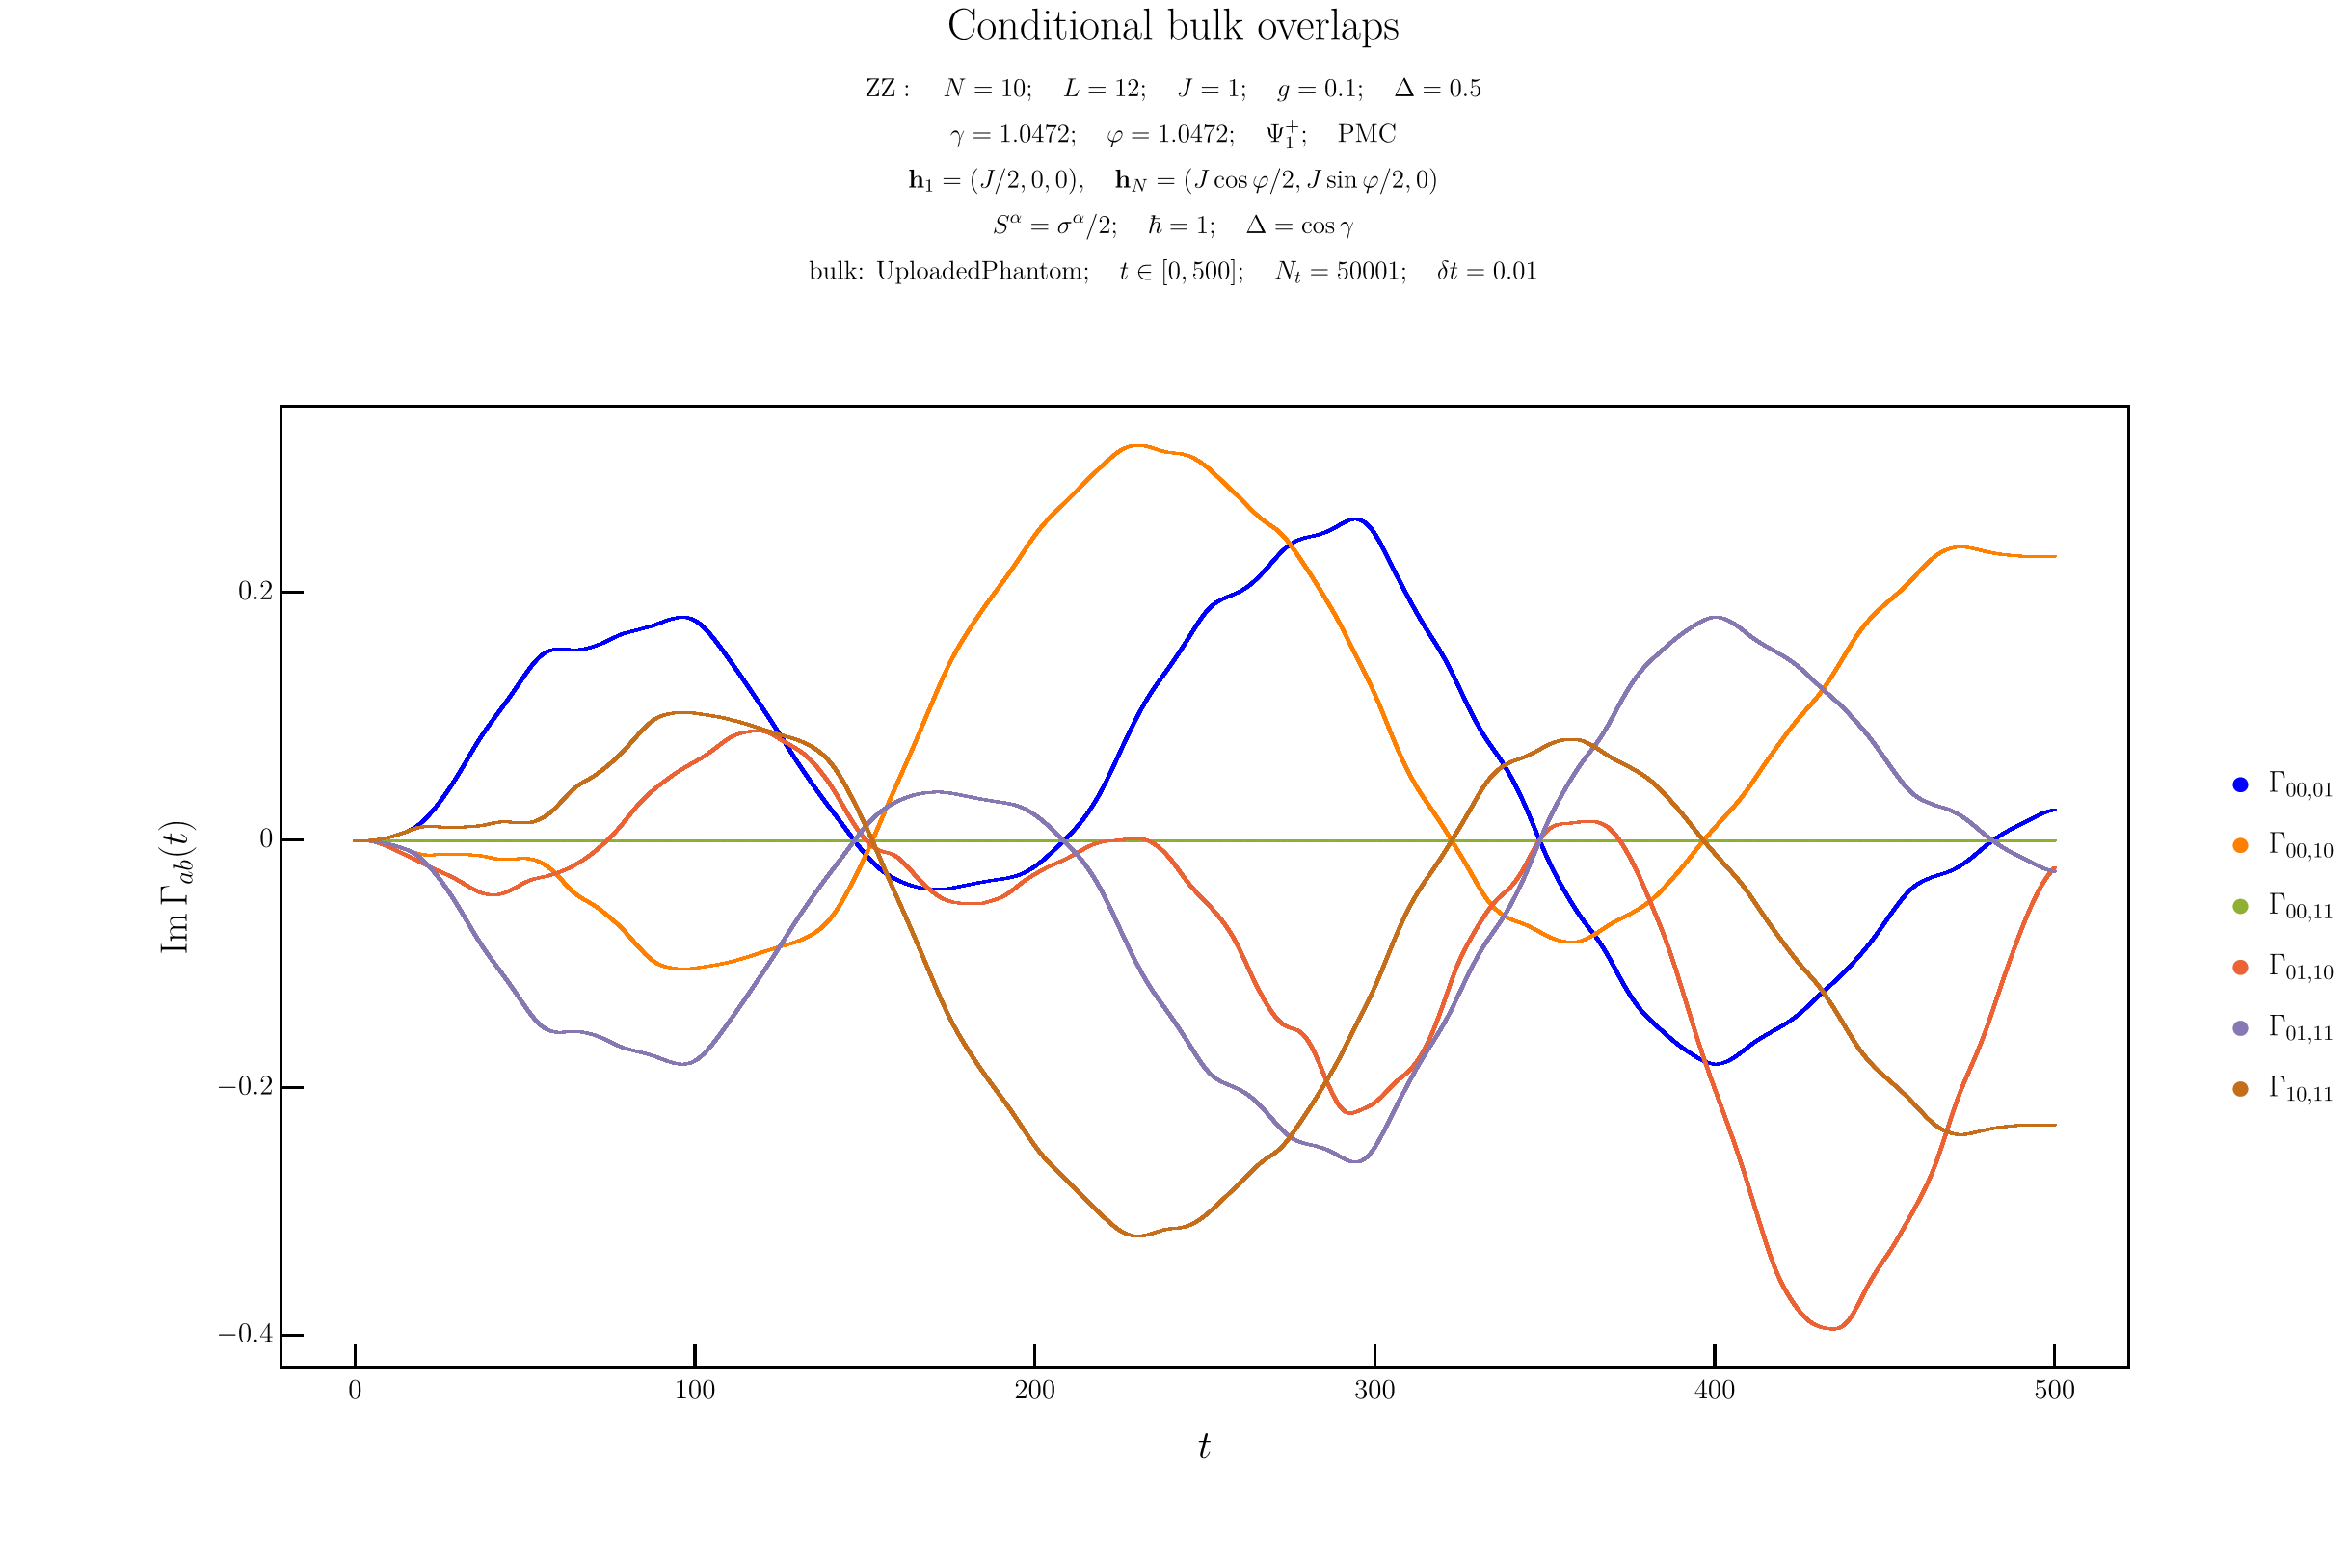
\includegraphics[width=\linewidth,height=0.50\textheight,keepaspectratio]{Phantom_ZZ_N10/Channel_Gamma_Im.png}
\end{column}
\end{columns}
\vspace{-4pt}
\[
\Gamma_{ab}(t)=\operatorname{Re}\Gamma_{ab}(t)+i\operatorname{Im}\Gamma_{ab}(t).
\]
\vspace{-6pt}
\begin{itemize}\setlength\itemsep{2pt}
\item \textbf{Exact reality of $\Gamma_{00,11}$:} $\operatorname{Im}\Gamma_{00,11}(t)\equiv 0$ (flat green line), while $\Gamma_{01,10}(t)$ is complex ($\operatorname{Im}\Gamma_{01,10}$ reaches $-0.395$ at $t=434.7$).
\item \textbf{Sign reversal of $\operatorname{Re}\Gamma_{01,10}$:} crosses zero across $t=222.60$ and reaches $-0.805$ at $t=300.25$ ($\lvert\Gamma_{01,10}\rvert=0.832$), driving the entanglement window.
\item \textbf{Conjugate single-flip pairs:} $(00,01),(01,11)$ and $(00,10),(10,11)$ overlap in $\operatorname{Re}\Gamma$ and mirror in $\operatorname{Im}\Gamma$.
\end{itemize}
\end{frame}

% ==============================================================
\begin{frame}{Symmetries of $\Gamma(t)$ and independent overlaps}
\footnotesize
\begin{columns}[T,totalwidth=\textwidth]
\begin{column}{0.49\textwidth}
\centering
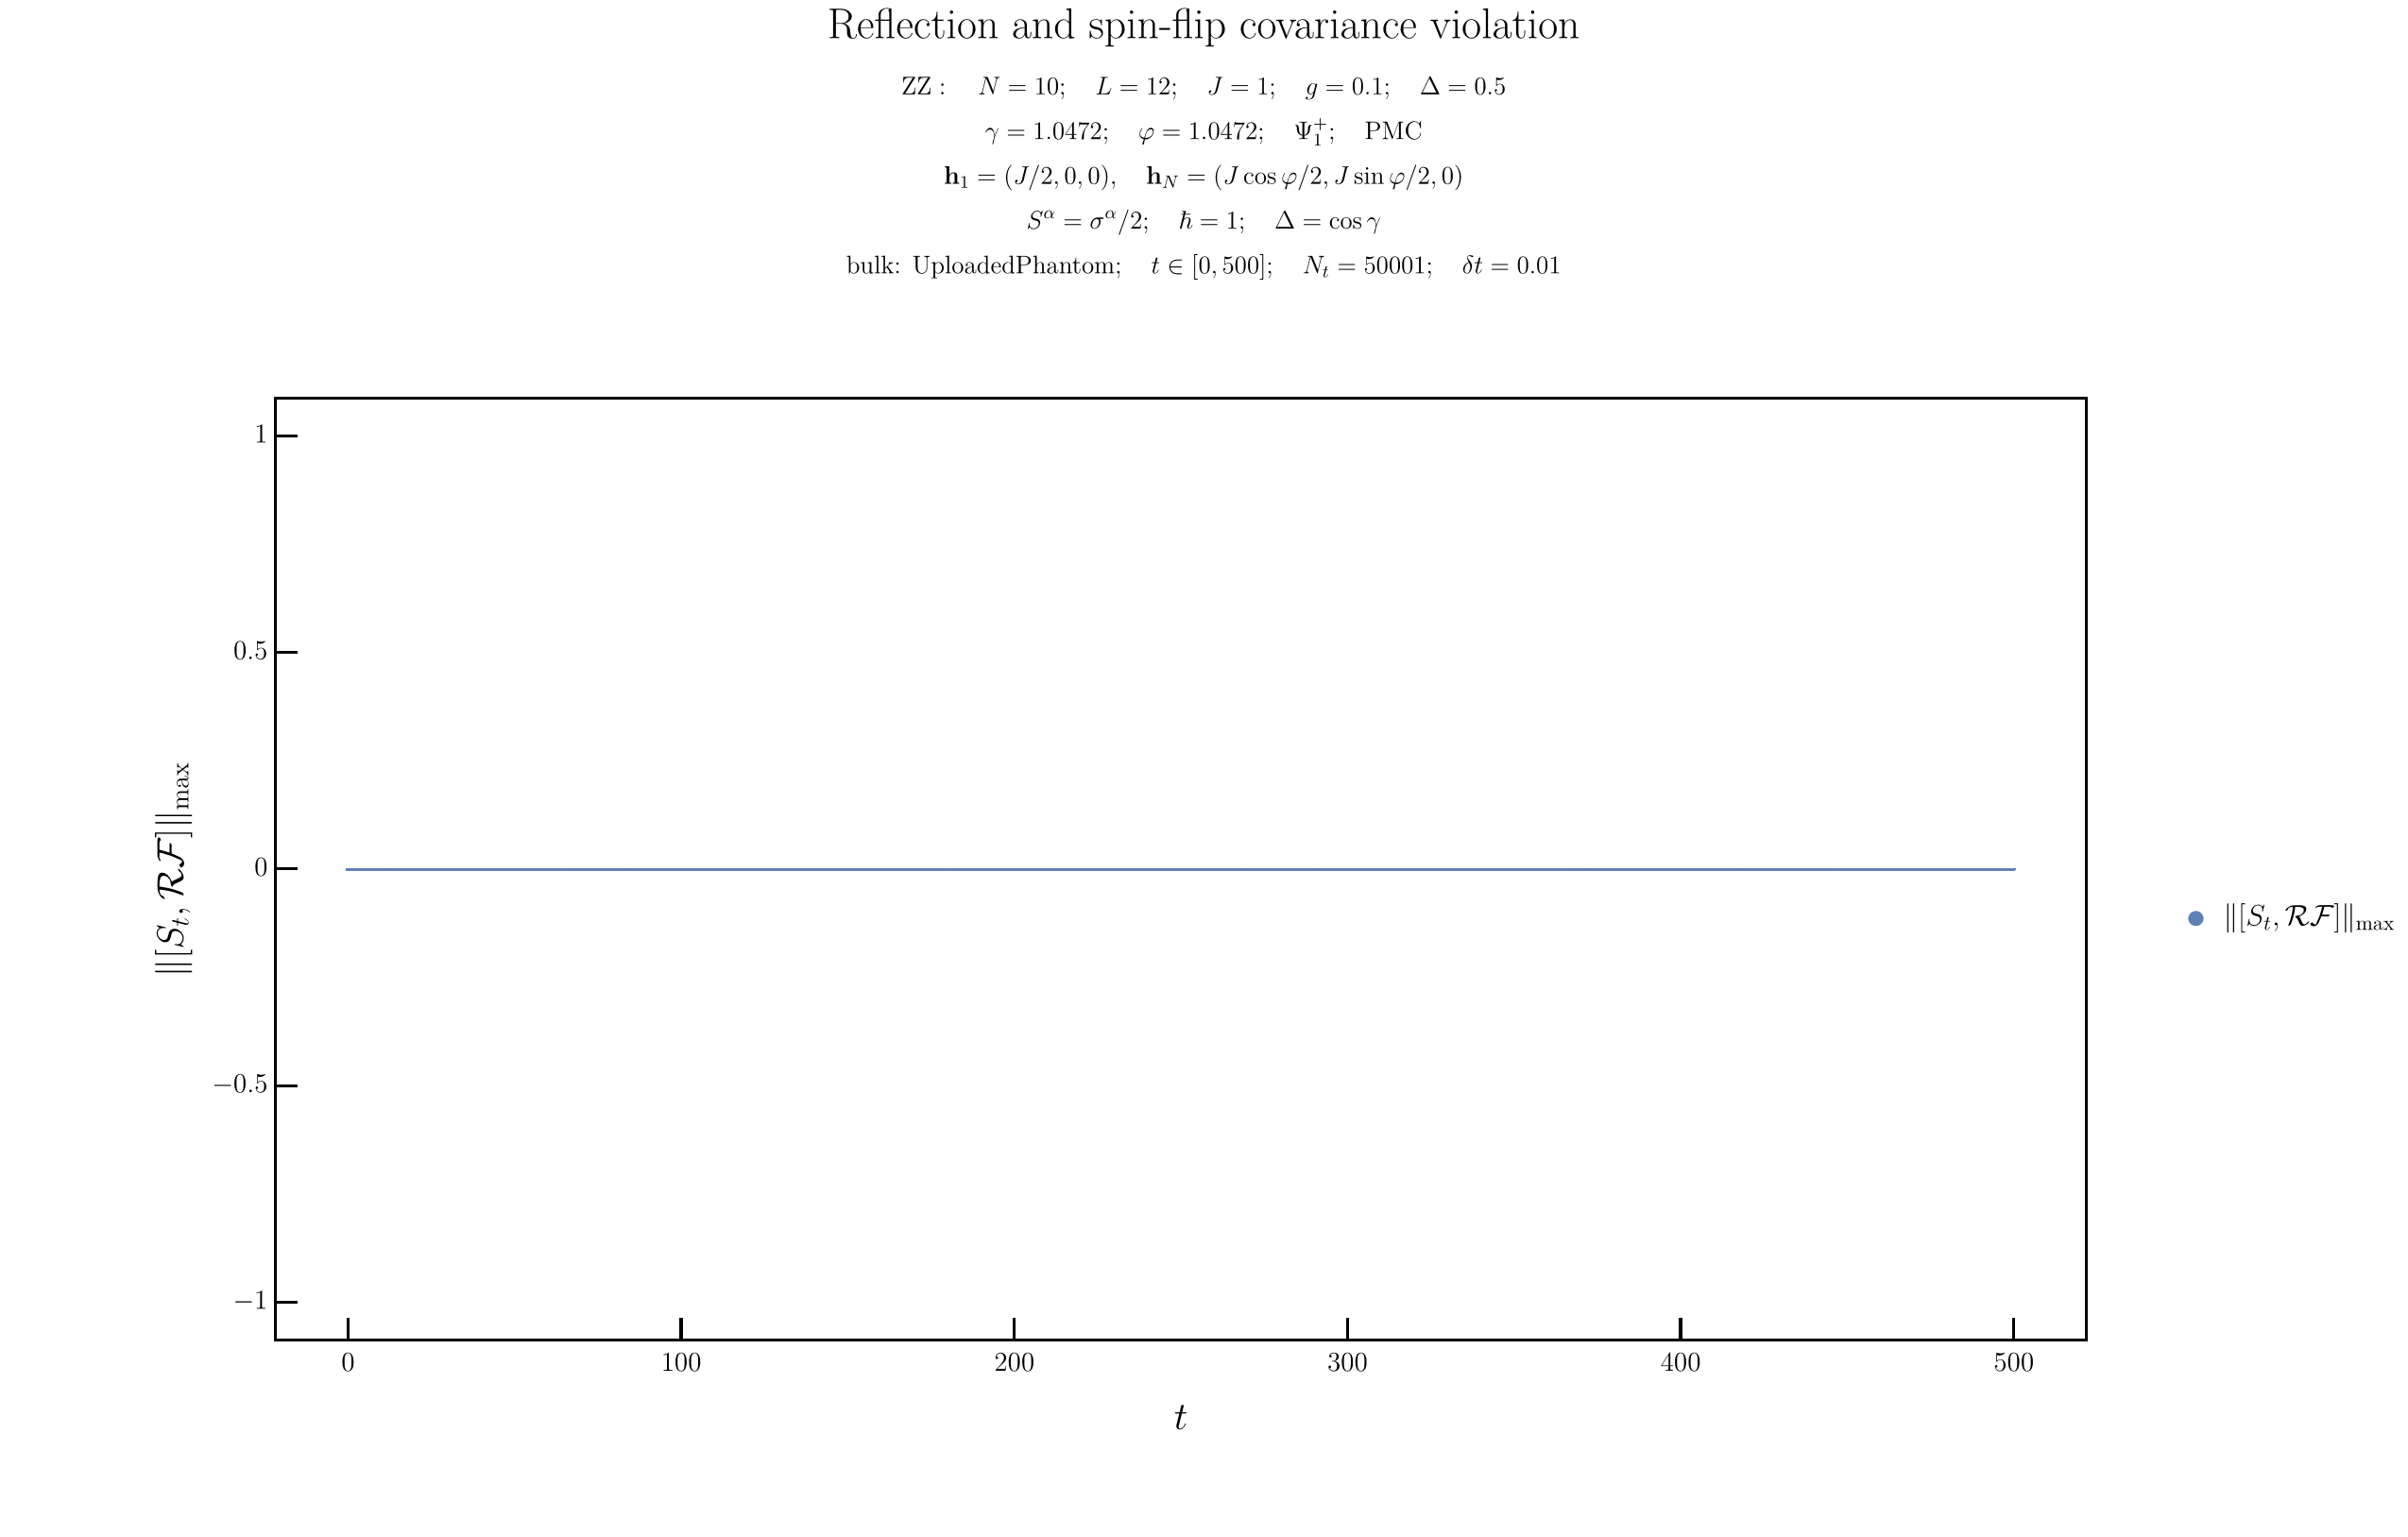
\includegraphics[width=\linewidth,height=0.47\textheight,keepaspectratio]{Phantom_ZZ_N10/Channel_RFCovarianceError.png}
\end{column}
\begin{column}{0.49\textwidth}
\centering
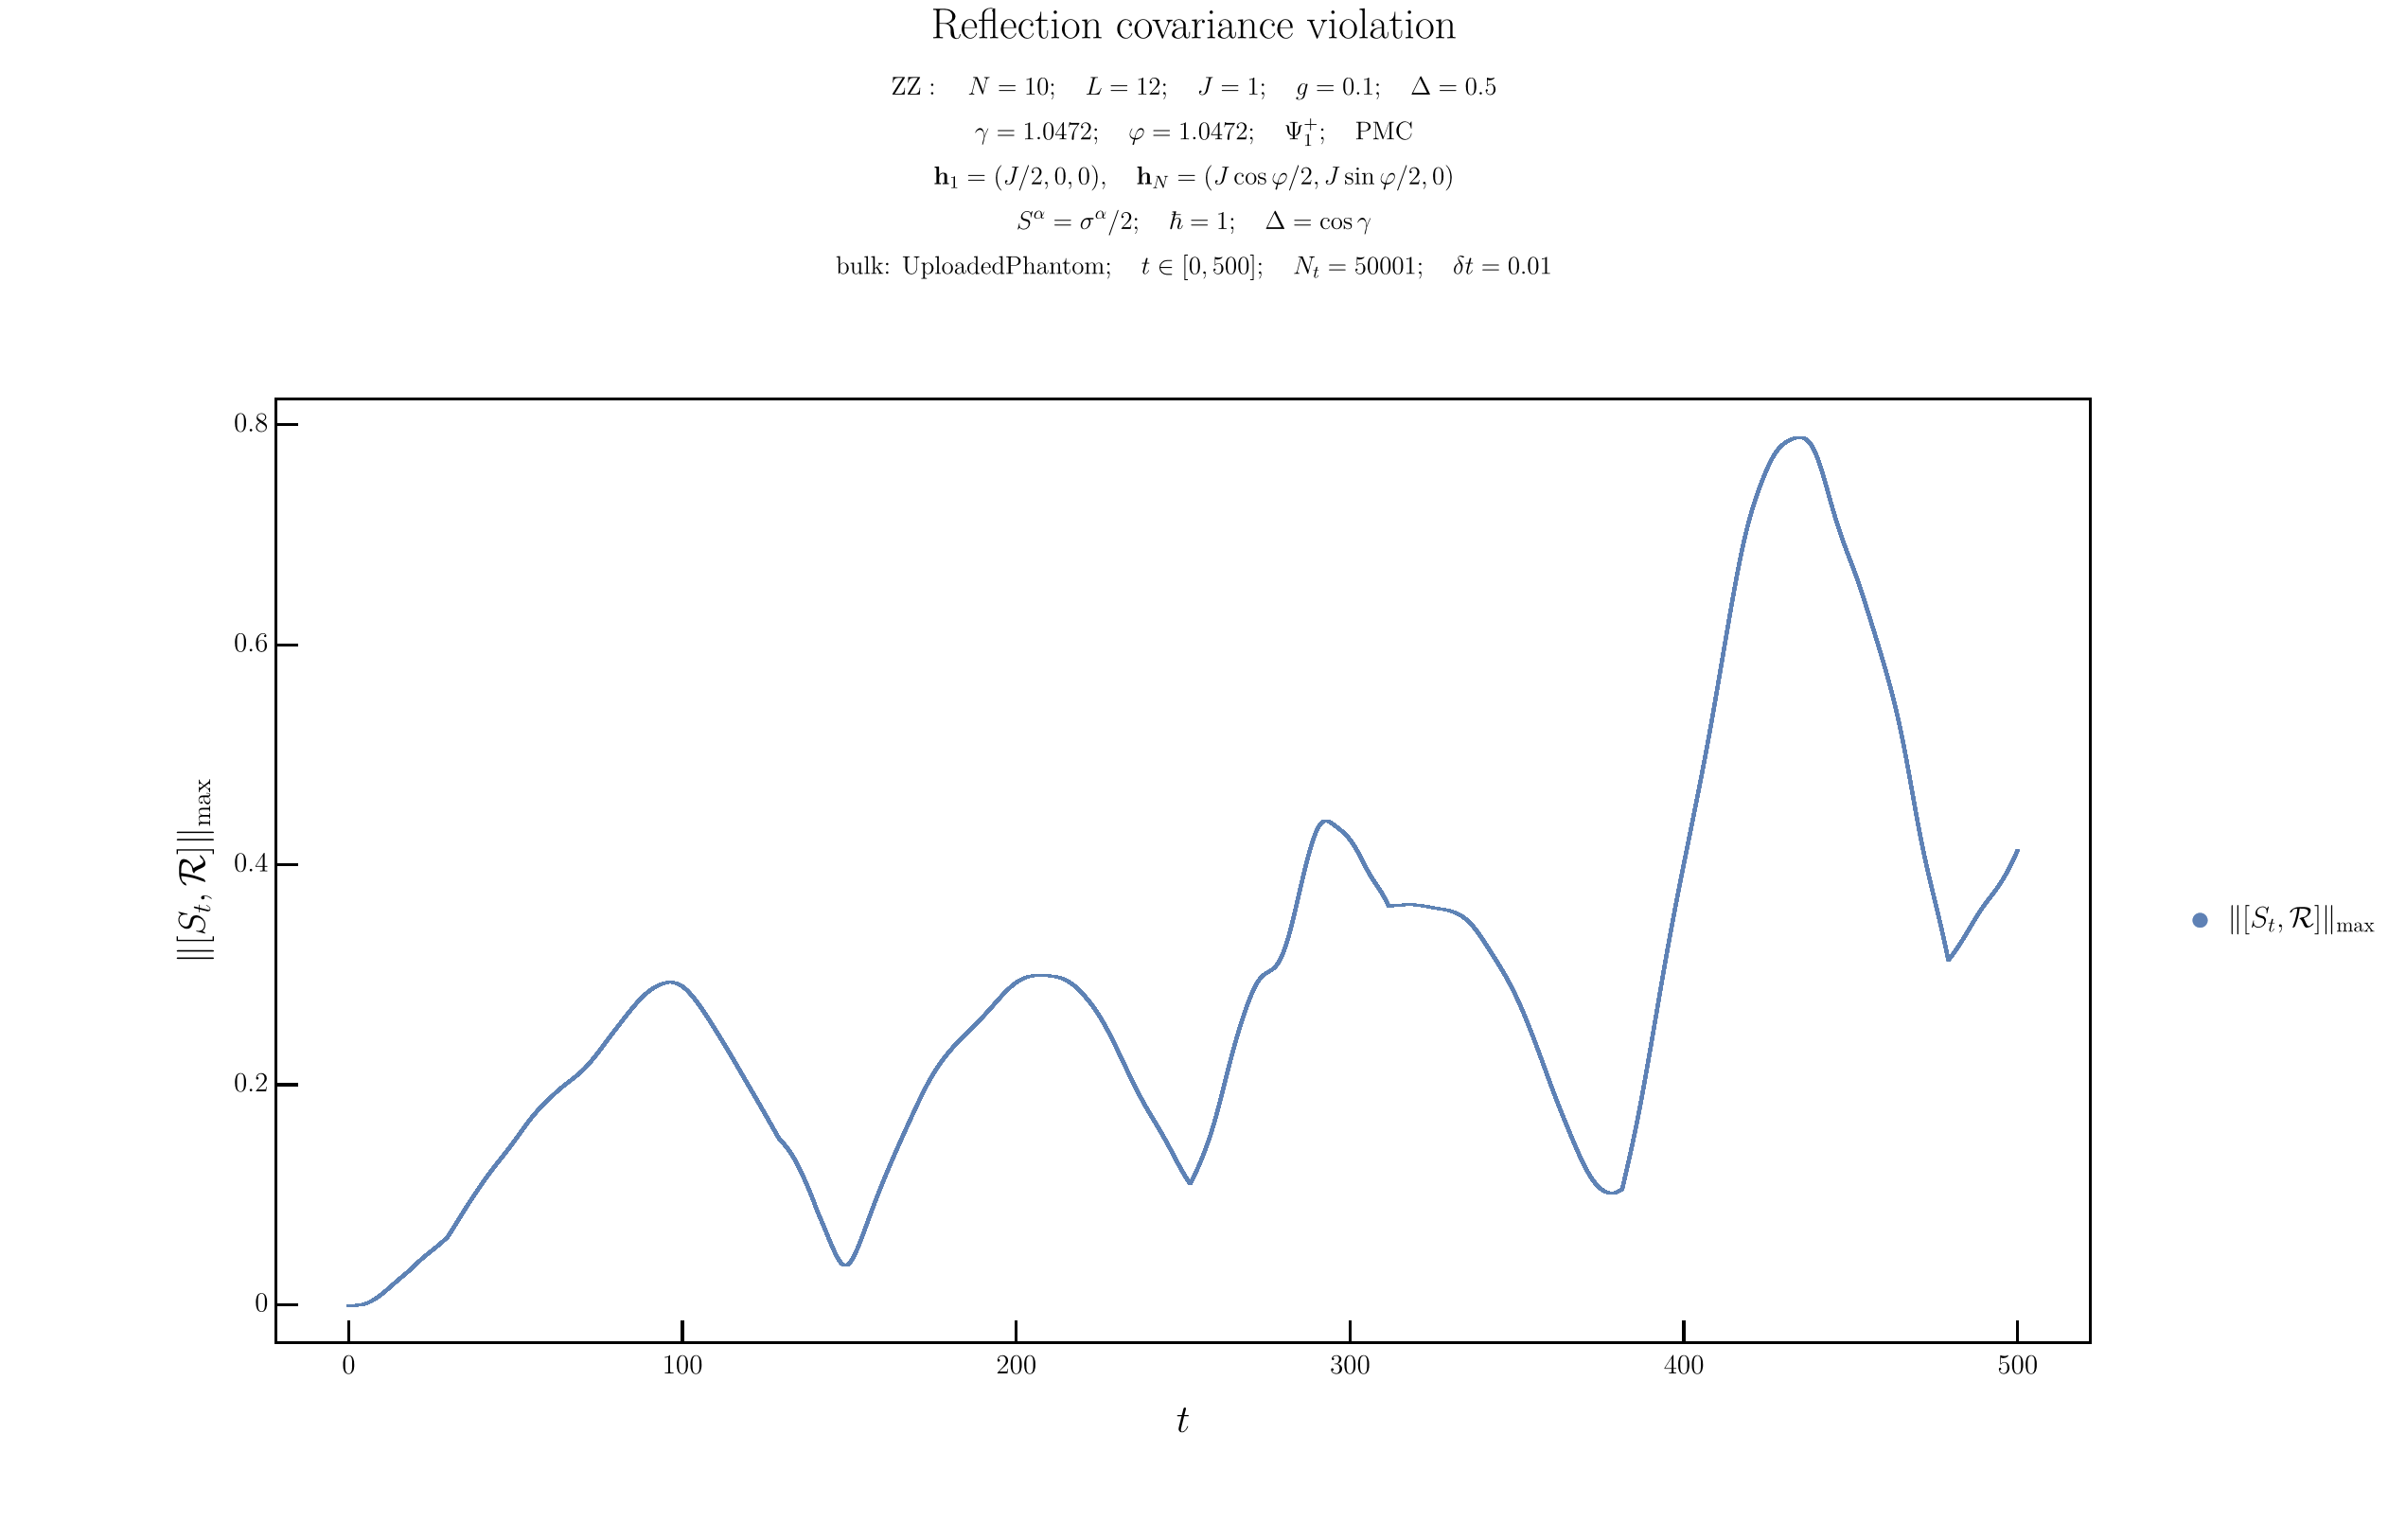
\includegraphics[width=\linewidth,height=0.47\textheight,keepaspectratio]{Phantom_ZZ_N10/Channel_ReflectionCovarianceError.png}
\end{column}
\end{columns}
\vspace{-4pt}
\[
W=\Theta T\text{ unitary}\implies \Gamma_{ab}(t)=\Gamma_{\sigma(\bar a)\sigma(\bar b)}(t)\iff \bigl[\St,\mathcal R\mathcal F\bigr]=0 .
\]
\vspace{-6pt}
\begin{itemize}\setlength\itemsep{2pt}
\item \textbf{$\mathcal R\mathcal F$ exact, $\mathcal R$ and $\mathcal F$ broken:} $\Theta=(\prod_j\sigma_j^x)K$ and $T=e^{-i\varphi M_z}\mathcal R_{\mathrm{bulk}}K$ are antiunitary (reversing $t$), so $\mathcal R$ and $\mathcal F$ alone fail identically: $\lVert[\St,\mathcal R]\rVert_{\max}\equiv\lVert[\St,\mathcal F]\rVert_{\max}\le 0.789$ ($t=434.7$).
\item \textbf{Four independent overlaps ($7$ real functions):} $\Gamma_{01,10}\in\mathbb C$, $\Gamma_{00,11}\in\mathbb R$, $\Gamma_{00,01}=\Gamma_{01,11}^*\in\mathbb C$, and $\Gamma_{00,10}=\Gamma_{10,11}^*\in\mathbb C$ (distinct: $\max_t\lvert\Gamma_{00,01}-\Gamma_{00,10}\rvert=0.413$; Appendix~2a).
\item \textbf{Exact eigenmode:} $\mathcal R\mathcal F=-1$ isolates $\ket{\Phi^-}=(\ket{00}-\ket{11})/\sqrt2$ with exact eigenvalue $1-\Gamma_{00,11}(t)$.
\end{itemize}
\end{frame}

% ==============================================================
\begin{frame}{Reduced edge coherences}
\begin{columns}[T,totalwidth=\textwidth]
\begin{column}{0.57\textwidth}
\centering
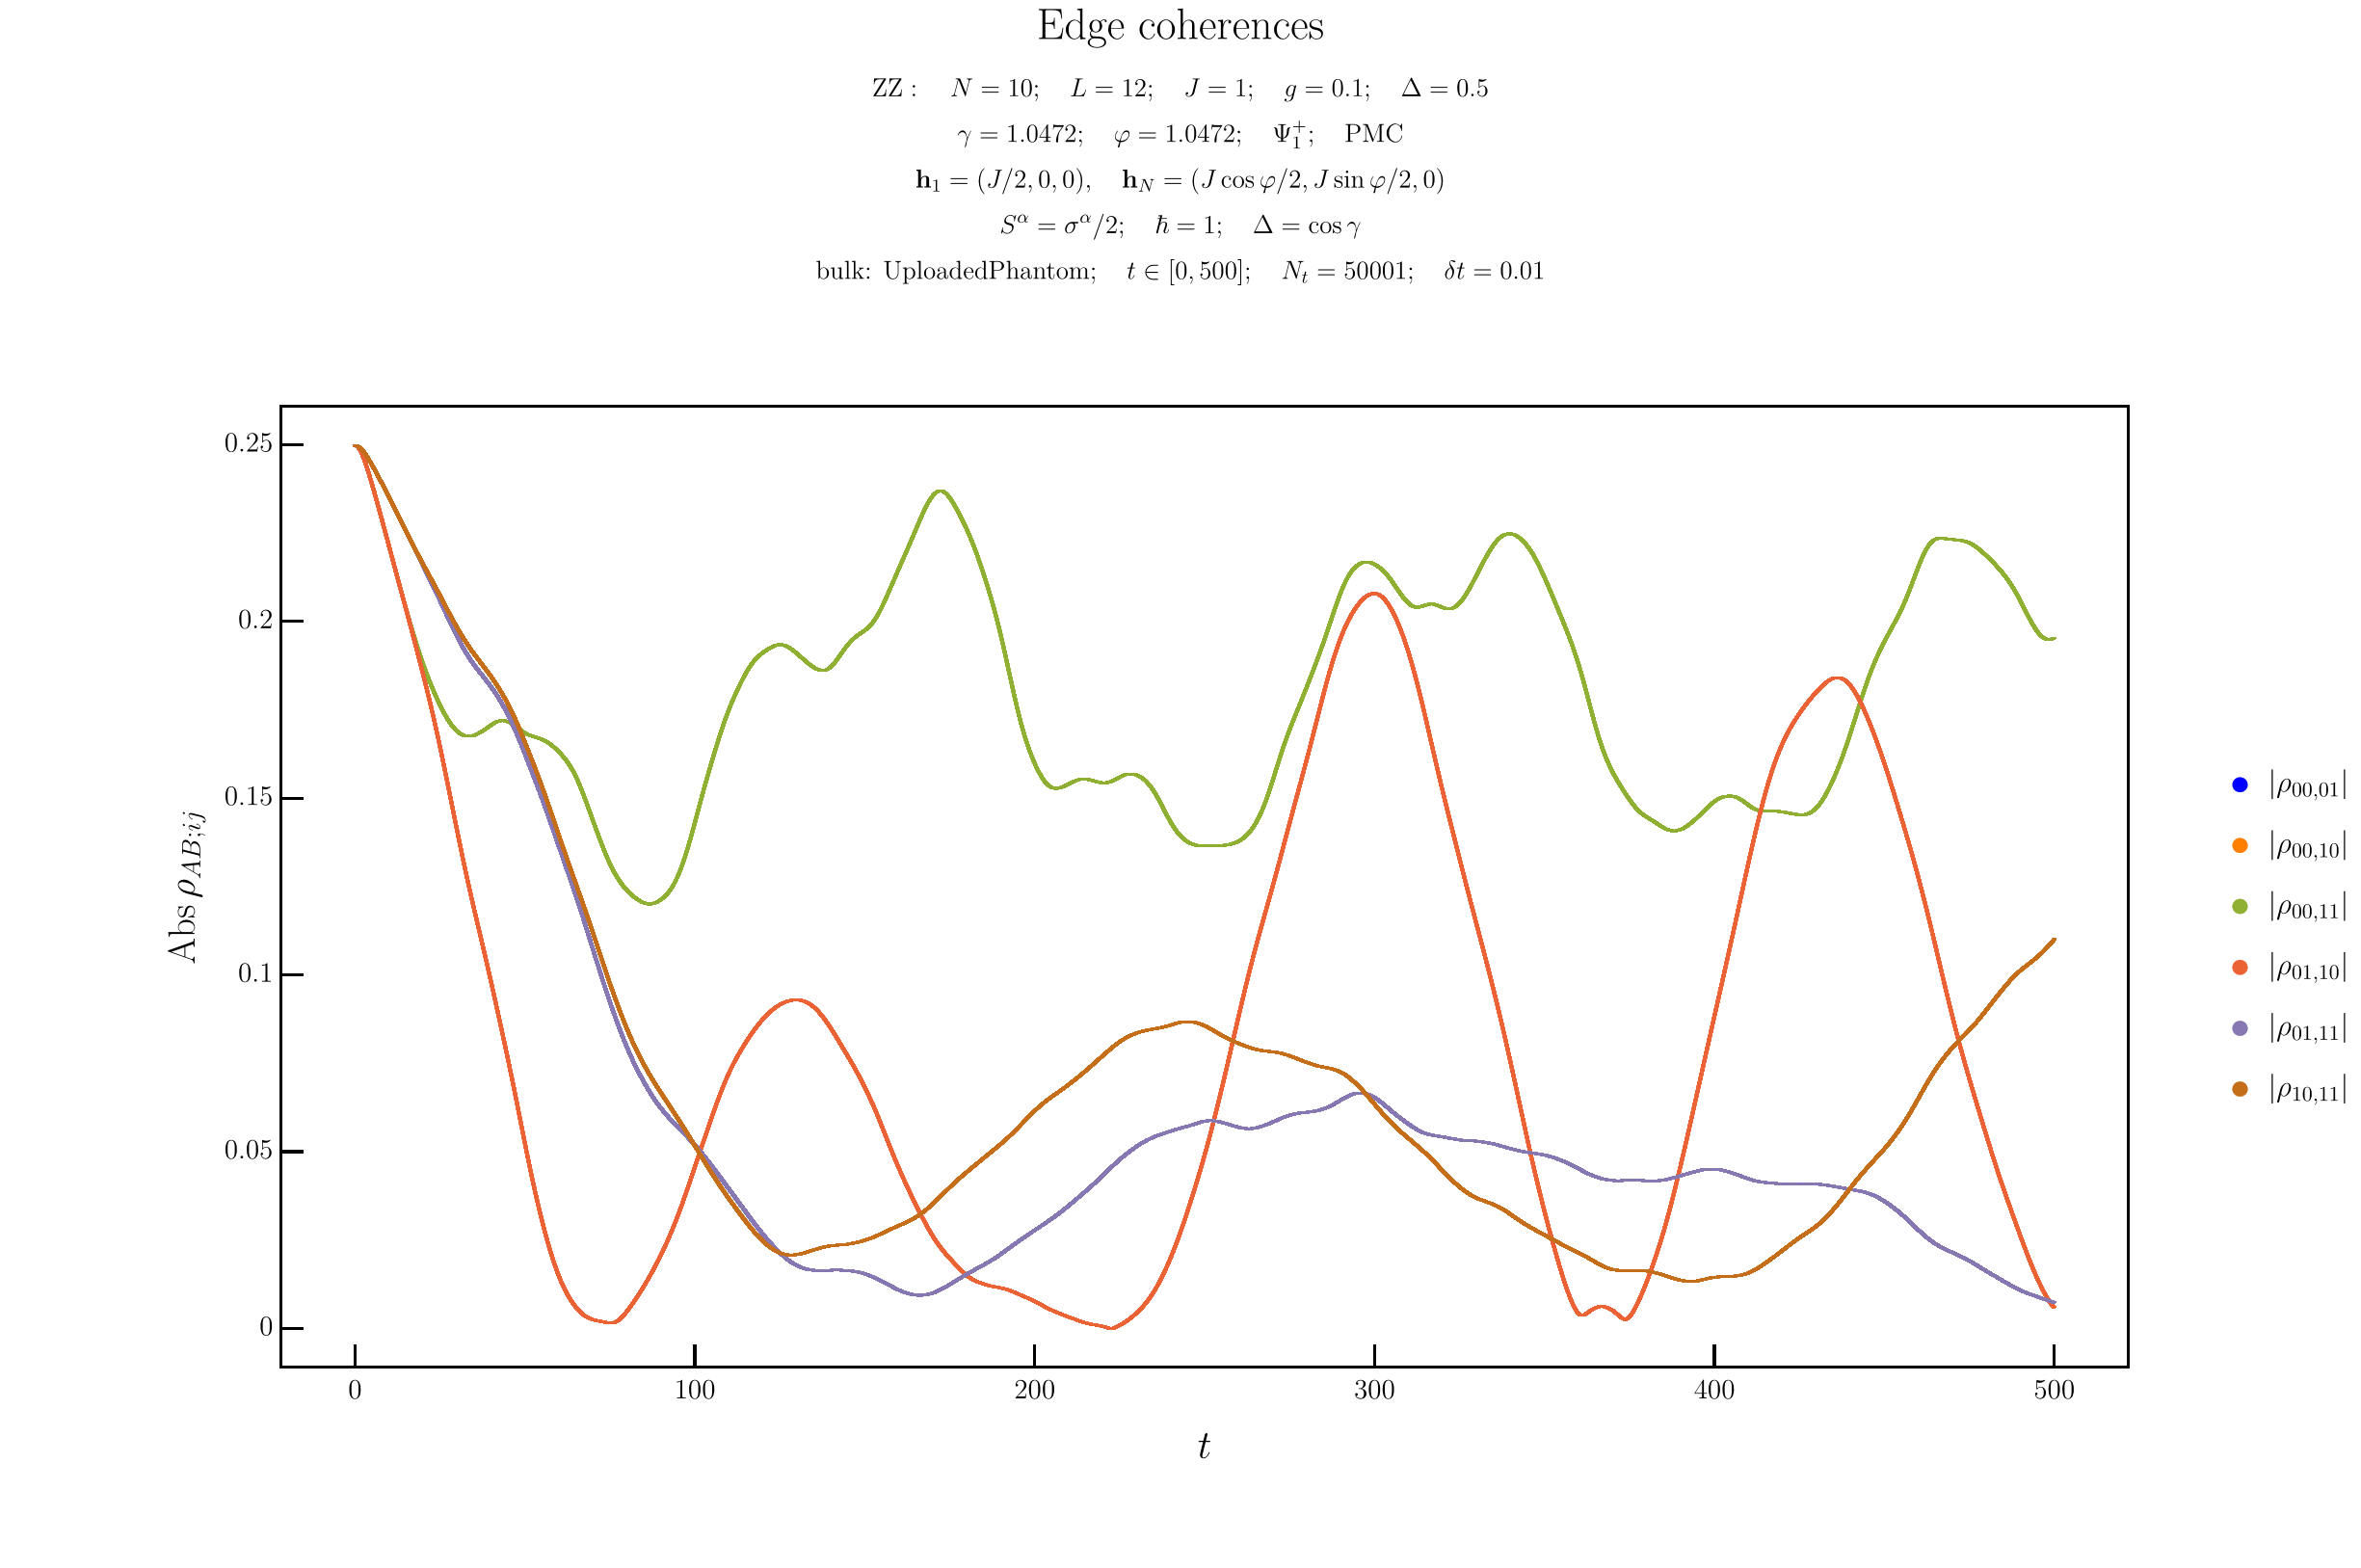
\includegraphics[width=\linewidth,height=0.77\textheight,keepaspectratio]{Phantom_ZZ_N10/State_EdgeCoherences_Abs.png}
\end{column}
\begin{column}{0.41\textwidth}
\footnotesize
\[
\lvert\rho_{AB;ab}(t)\rvert=\frac14\,\lvert\Gamma_{ab}(t)\rvert\qquad(a<b).
\]
\begin{itemize}\setlength\itemsep{5pt}
\item \textbf{Scaled mirror of $\lvert\Gamma_{ab}\rvert$:} every curve equals $1/4$ of \texttt{Channel\_Gamma\_Abs} (verified to $8\times 10^{-13}$), starting at $0.25$ while all four populations remain $0.25$.
\item \textbf{Smooth near-zero:} $\lvert\rho_{01,10}(t)\rvert$ dips smoothly to $2.67\times 10^{-5}$ at $t=222.60$ and revives to $0.208$ at $t=299.9$.
\item \textbf{Hidden pairs:} $\lvert\rho_{00,01}\rvert=\lvert\rho_{01,11}\rvert$ and $\lvert\rho_{00,10}\rvert=\lvert\rho_{10,11}\rvert$ overlap exactly.
\end{itemize}
\end{column}
\end{columns}
\end{frame}

% ==============================================================
\begin{frame}{Single-edge Bloch dynamics}
\footnotesize
\begin{columns}[T,totalwidth=\textwidth]
\begin{column}{0.49\textwidth}
\centering
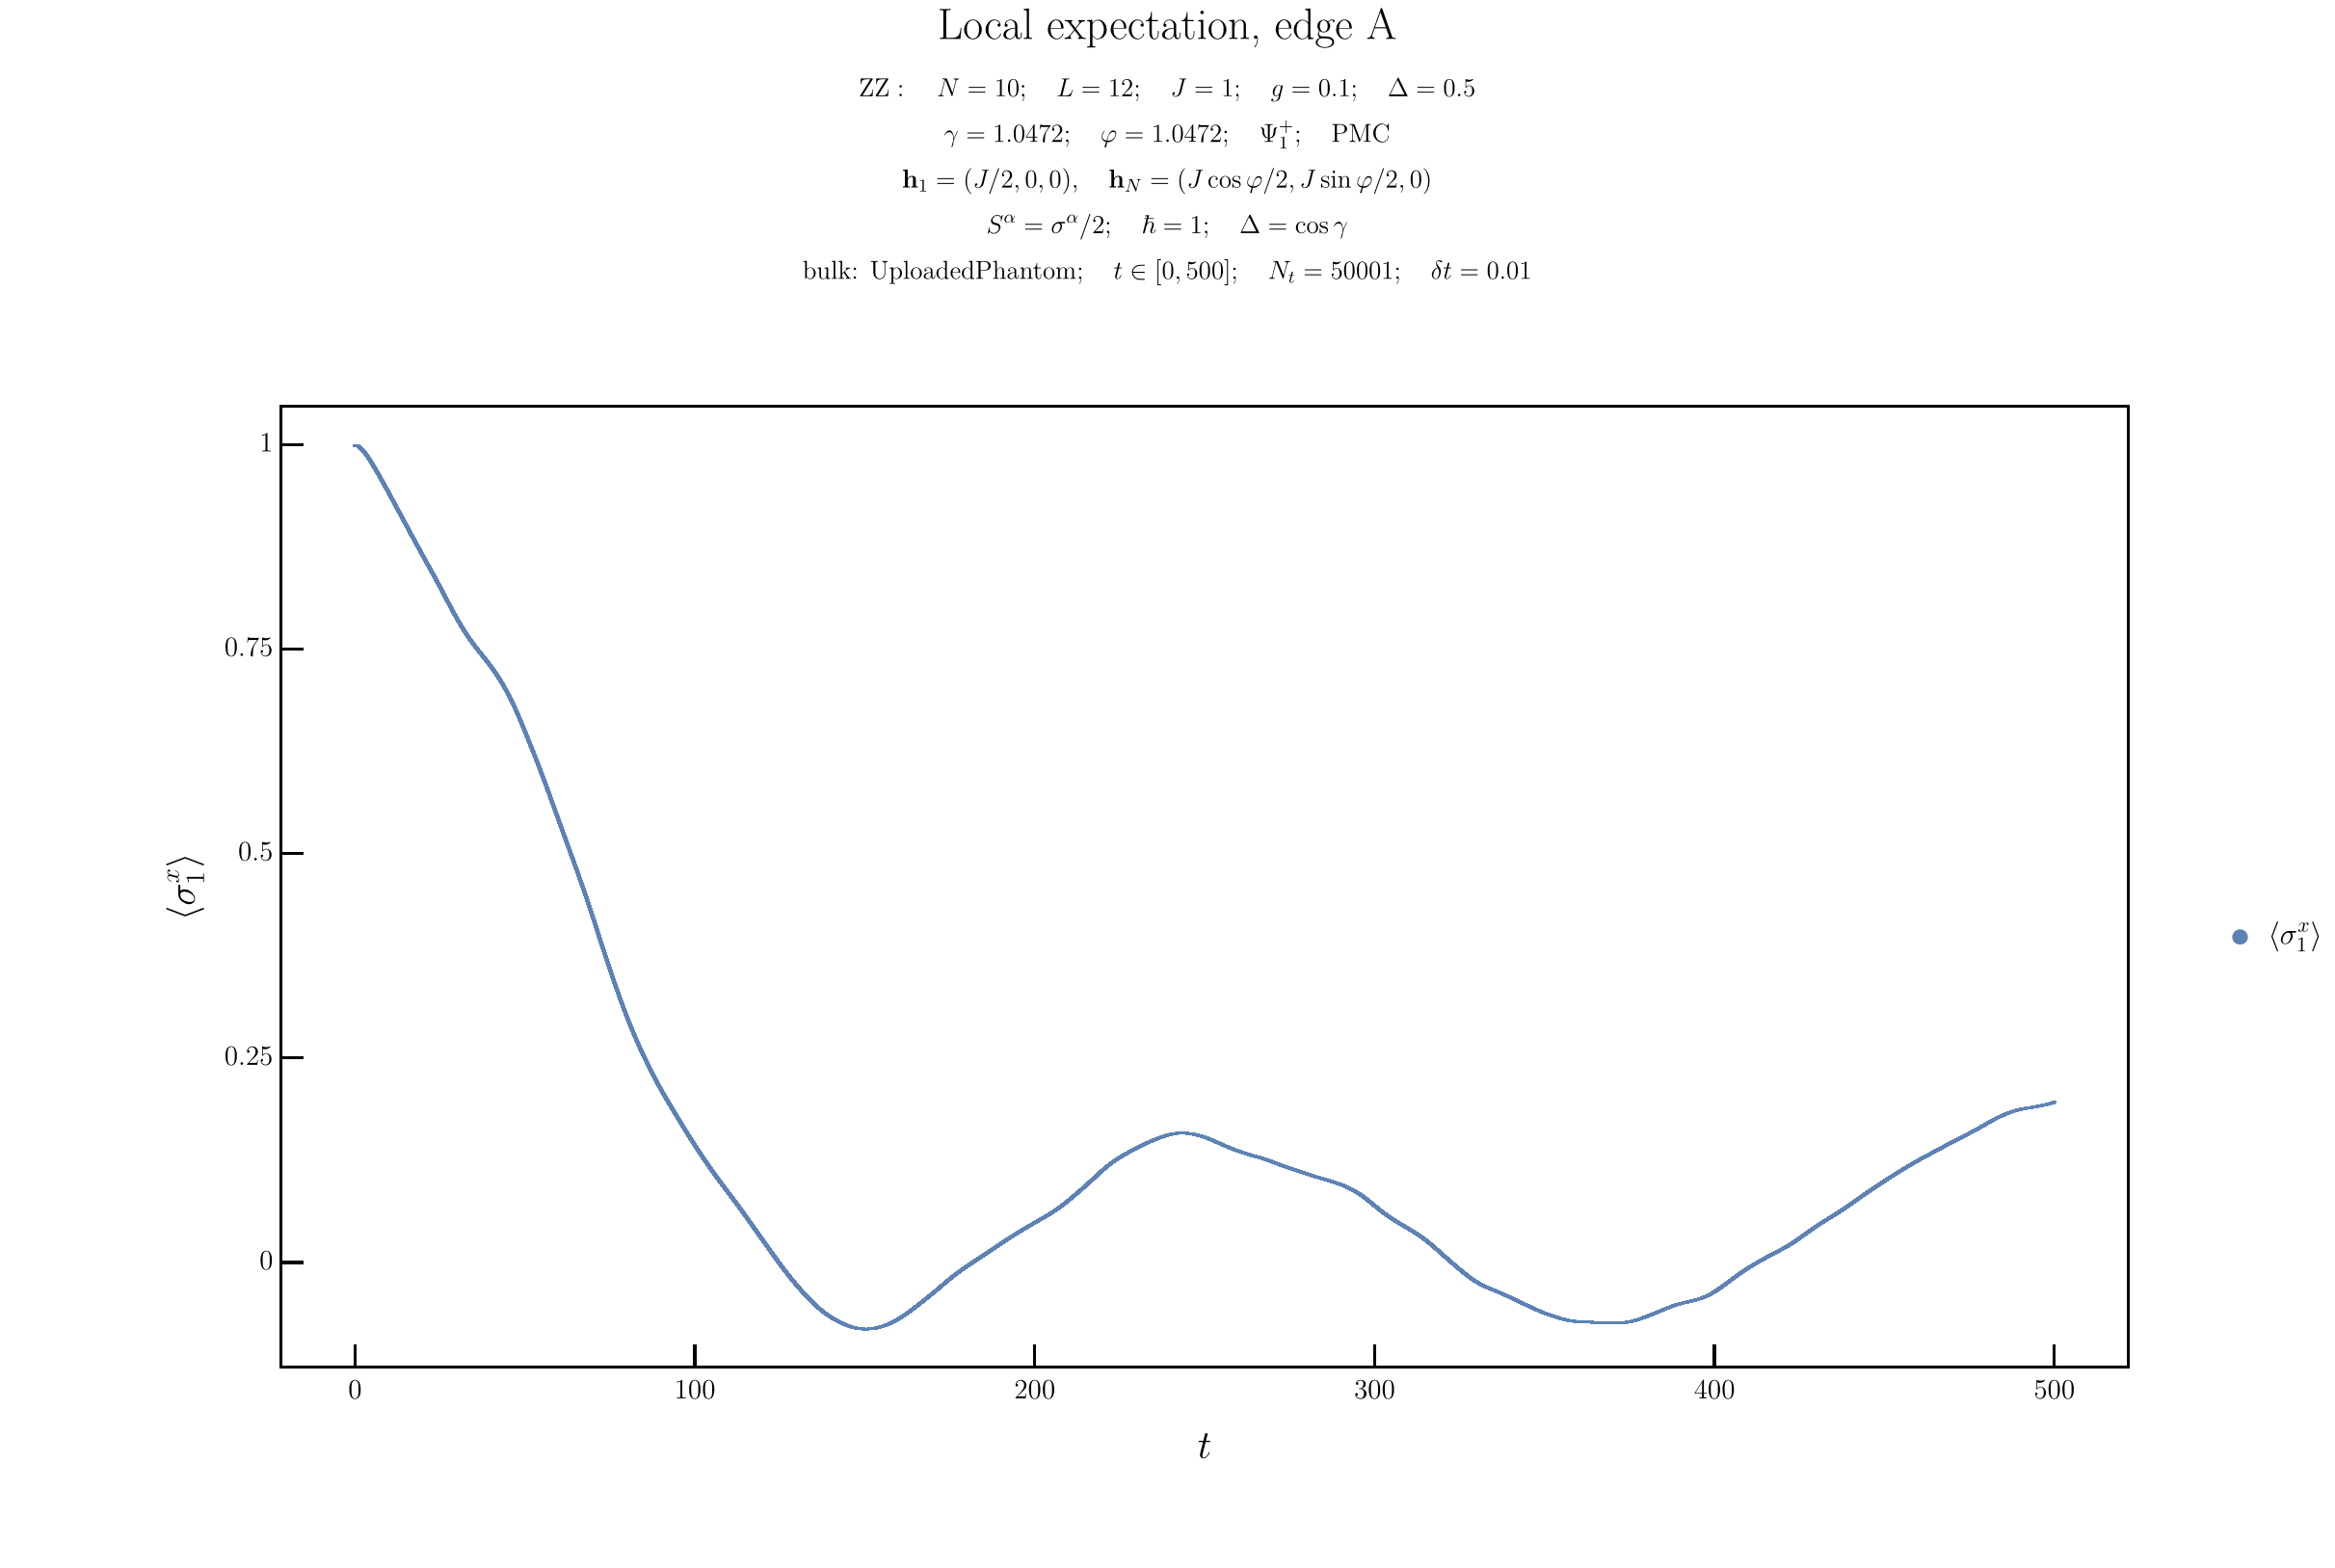
\includegraphics[width=\linewidth,height=0.49\textheight,keepaspectratio]{Phantom_ZZ_N10/State_LocalAX.png}
\end{column}
\begin{column}{0.49\textwidth}
\centering
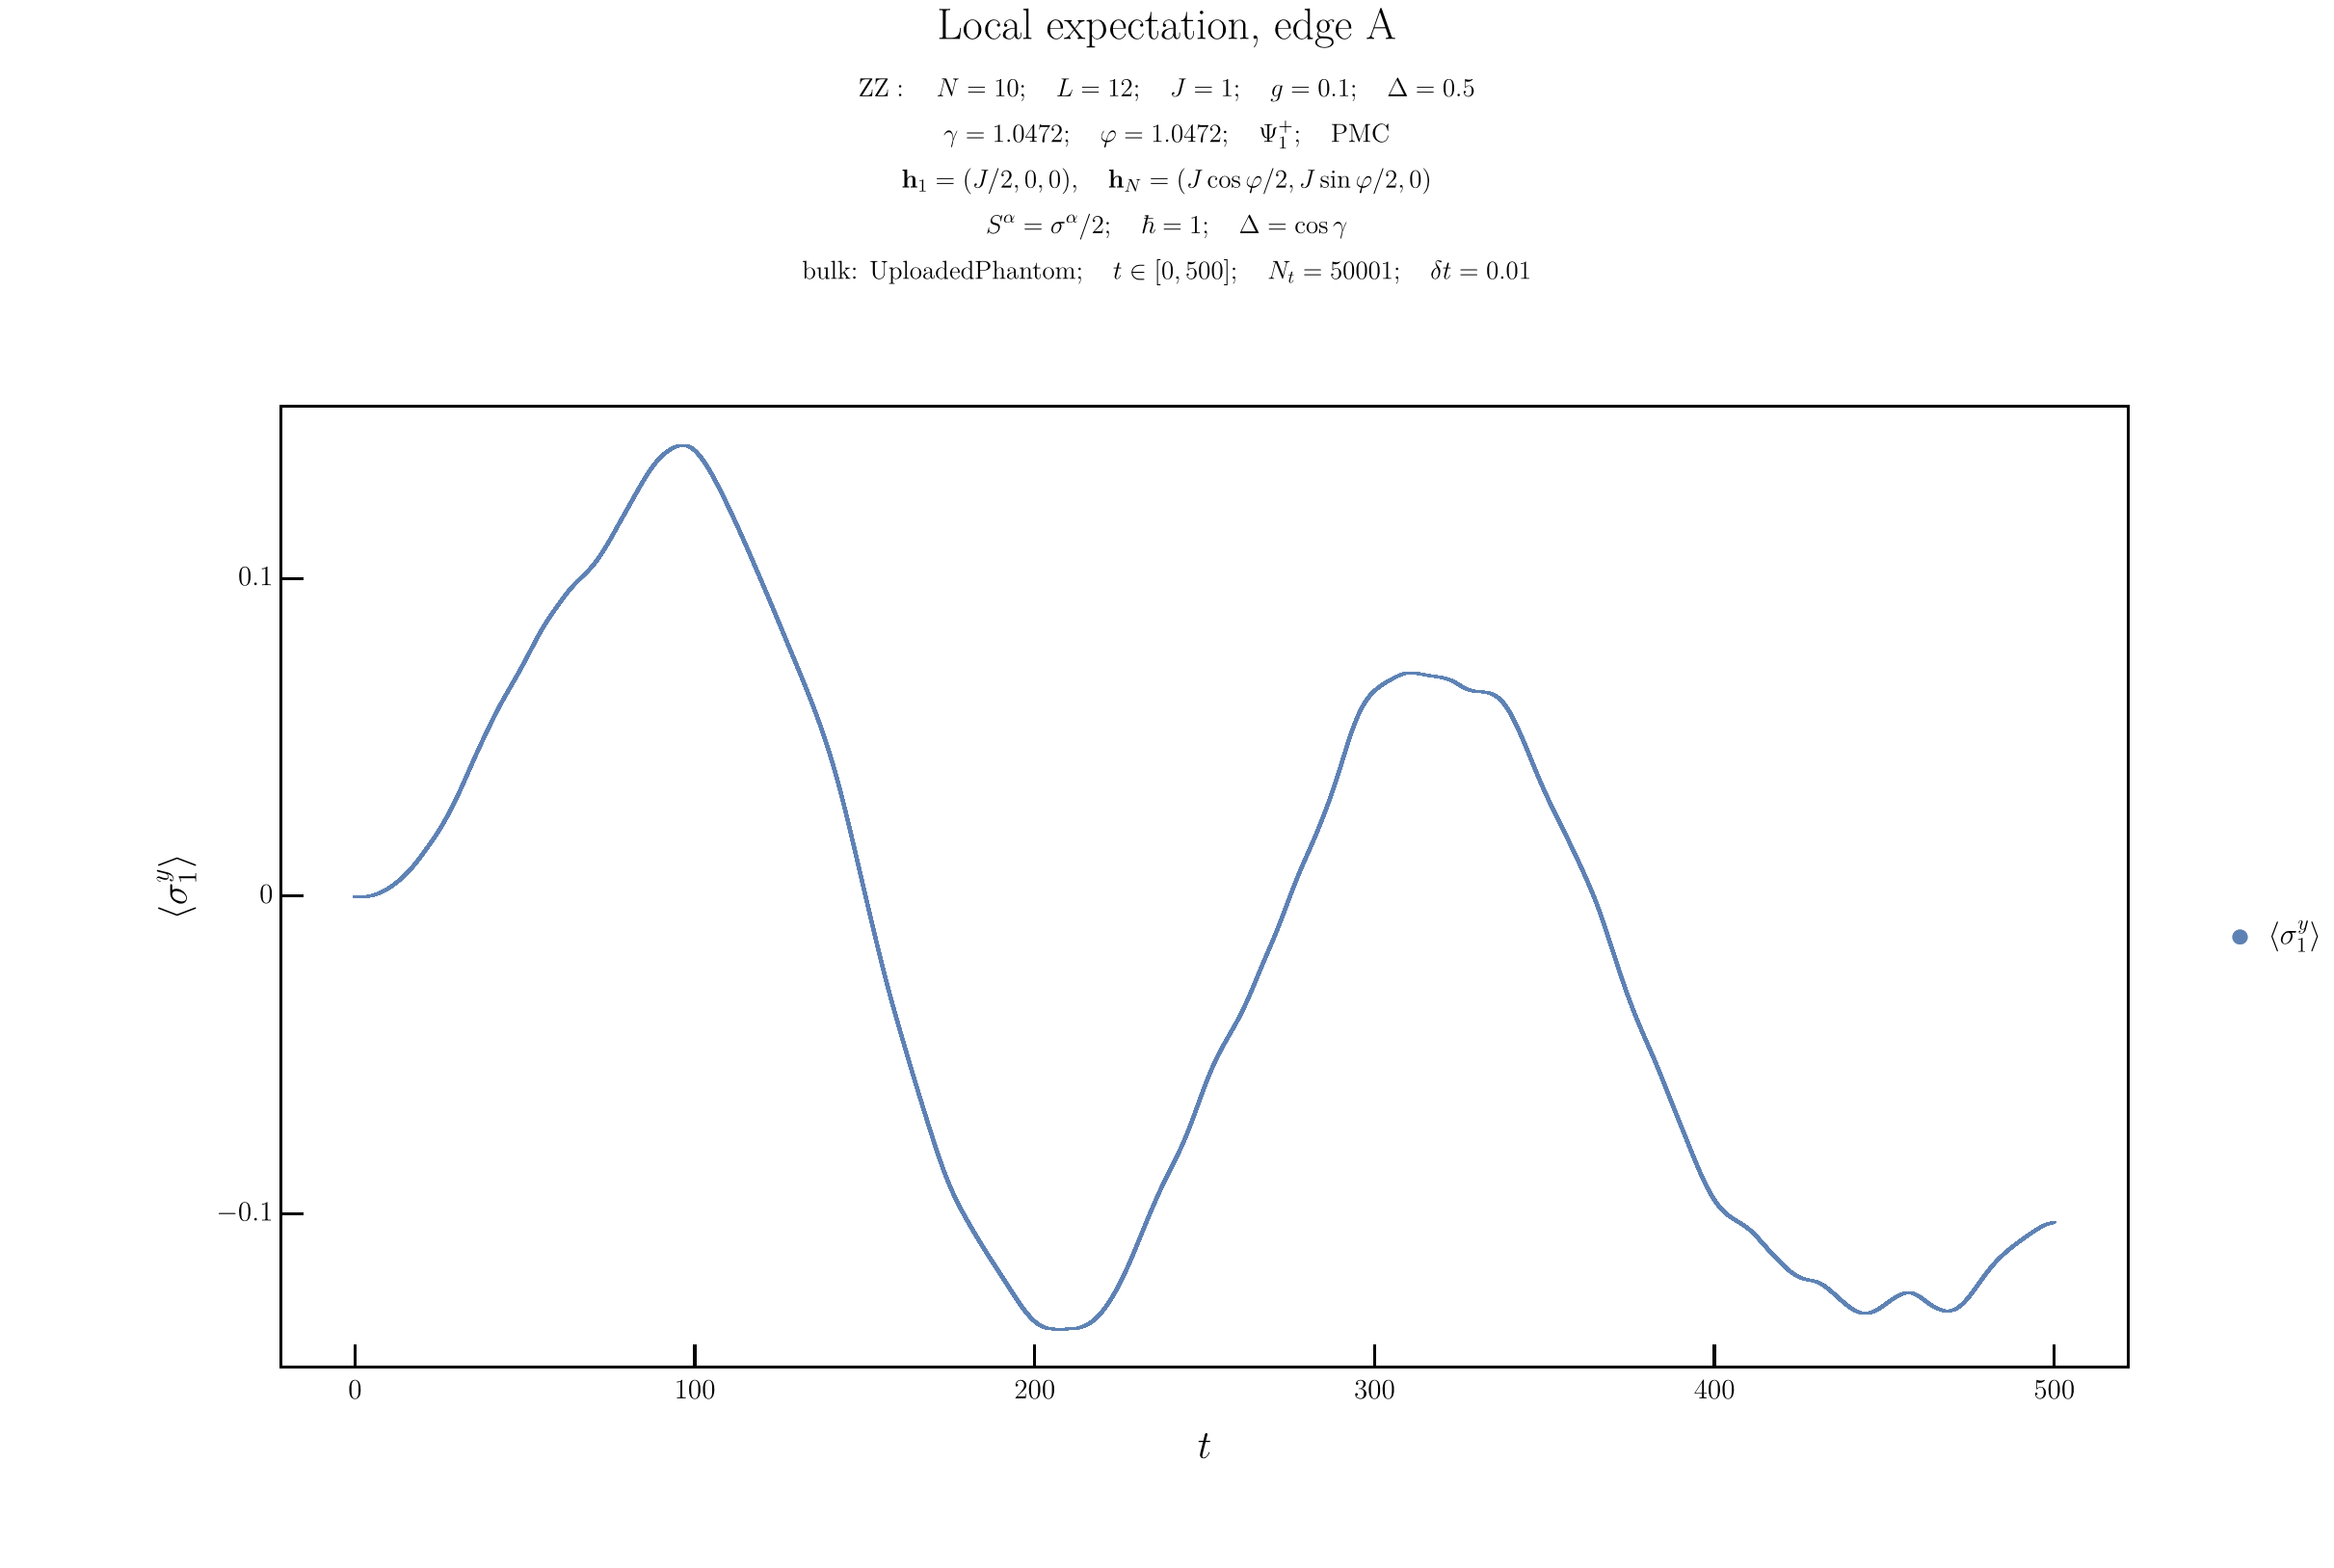
\includegraphics[width=\linewidth,height=0.49\textheight,keepaspectratio]{Phantom_ZZ_N10/State_LocalAY.png}
\end{column}
\end{columns}
\vspace{-4pt}
\[
\langle\sigma_A^x\rangle=\tfrac12\operatorname{Re}\bigl(\Gamma_{00,10}+\Gamma_{01,11}\bigr),\qquad
\langle\sigma_A^y\rangle=-\tfrac12\operatorname{Im}\bigl(\Gamma_{00,10}+\Gamma_{01,11}\bigr),\qquad
\langle\sigma_A^z\rangle=0 .
\]
\vspace{-6pt}
\begin{itemize}\setlength\itemsep{2pt}
\item \textbf{Edge $A$ vs.\ edge $B$:} $\Gamma_{00,01}+\Gamma_{10,11}=(\Gamma_{00,10}+\Gamma_{01,11})^*$ gives $\rho_B(t)=\rho_A(t)^*$, hence $\langle\sigma_B^x\rangle=+\langle\sigma_A^x\rangle$ and $\langle\sigma_B^y\rangle=-\langle\sigma_A^y\rangle$ ($\sigma_1\equiv\sigma_A$ in plot labels).
\item \textbf{Local dephasing:} $\langle\sigma_A^x\rangle$ decays from $1$ into $[-0.081,0.20]$ for $t\gtrsim 100$, while chiral precession induces $\langle\sigma_A^y\rangle\in[-0.136,+0.142]$, leaving $\rho_{A,B}(t)$ close to $I_2/2$.
\end{itemize}
\end{frame}

% ==============================================================
\begin{frame}{Edge entropies and local mixedness}
\begin{columns}[T,totalwidth=\textwidth]
\begin{column}{0.57\textwidth}
\centering
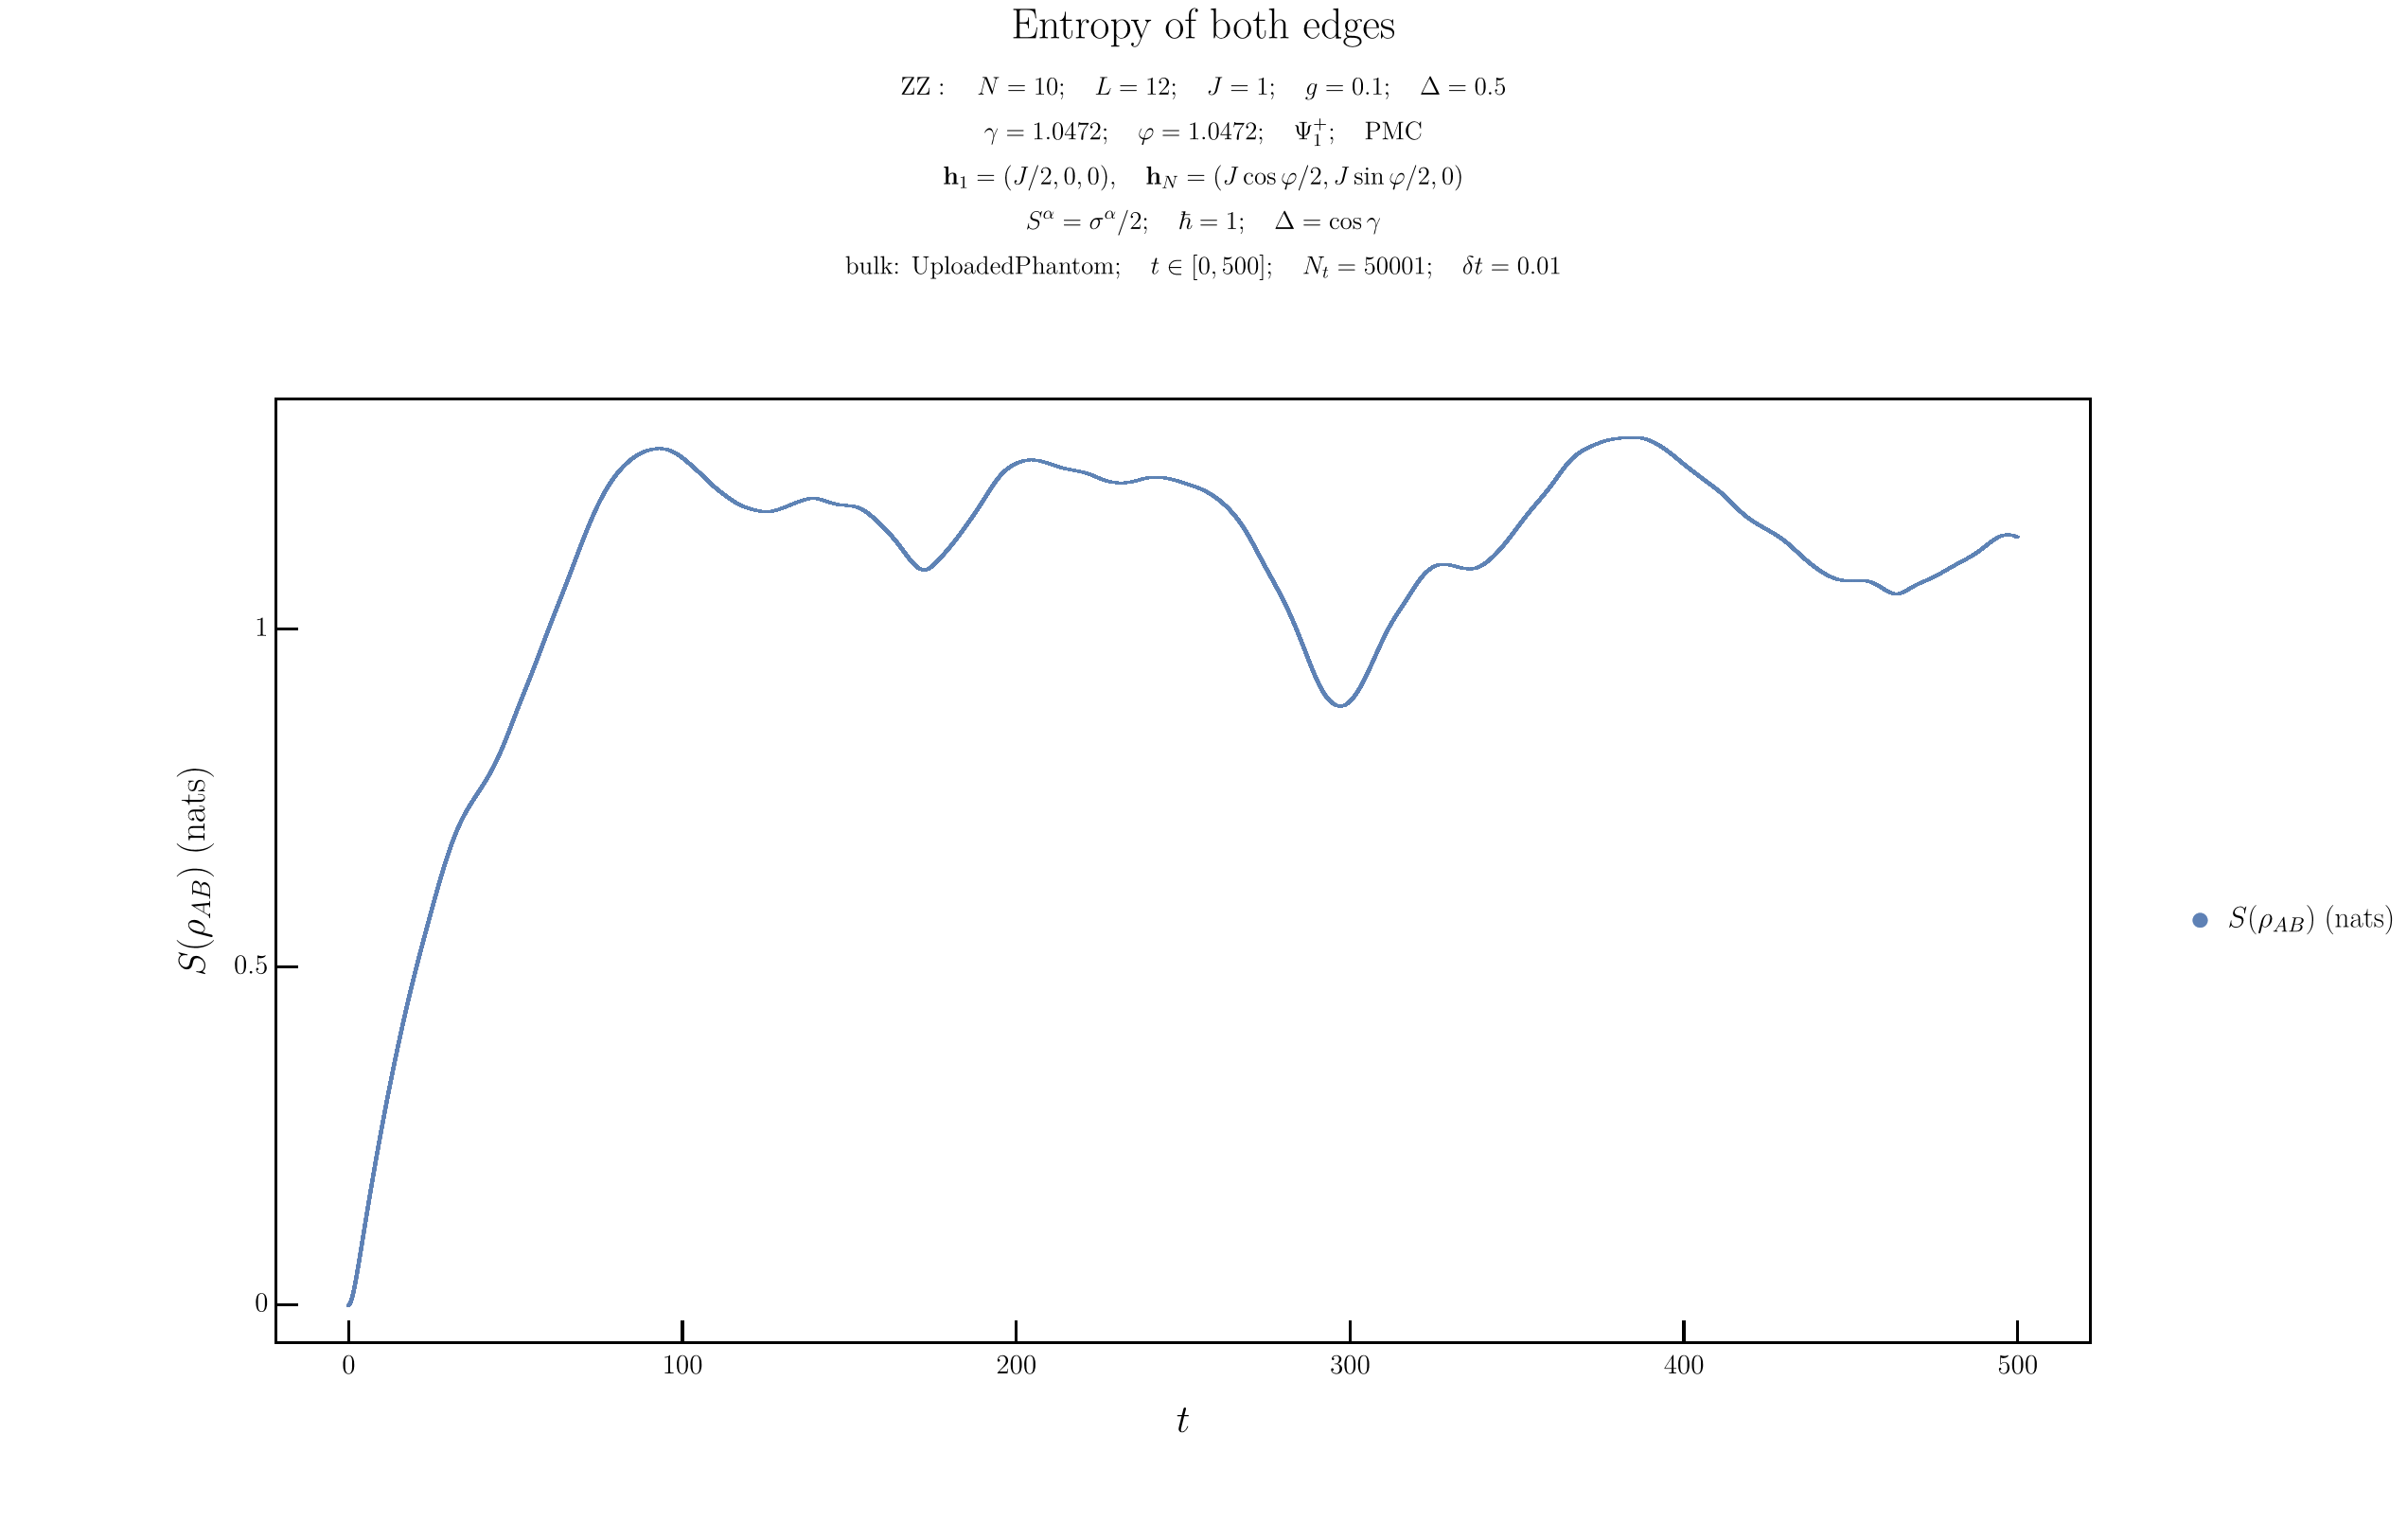
\includegraphics[width=\linewidth,height=0.41\textheight,keepaspectratio]{Phantom_ZZ_N10/State_EntropyAB.png}\\[2pt]
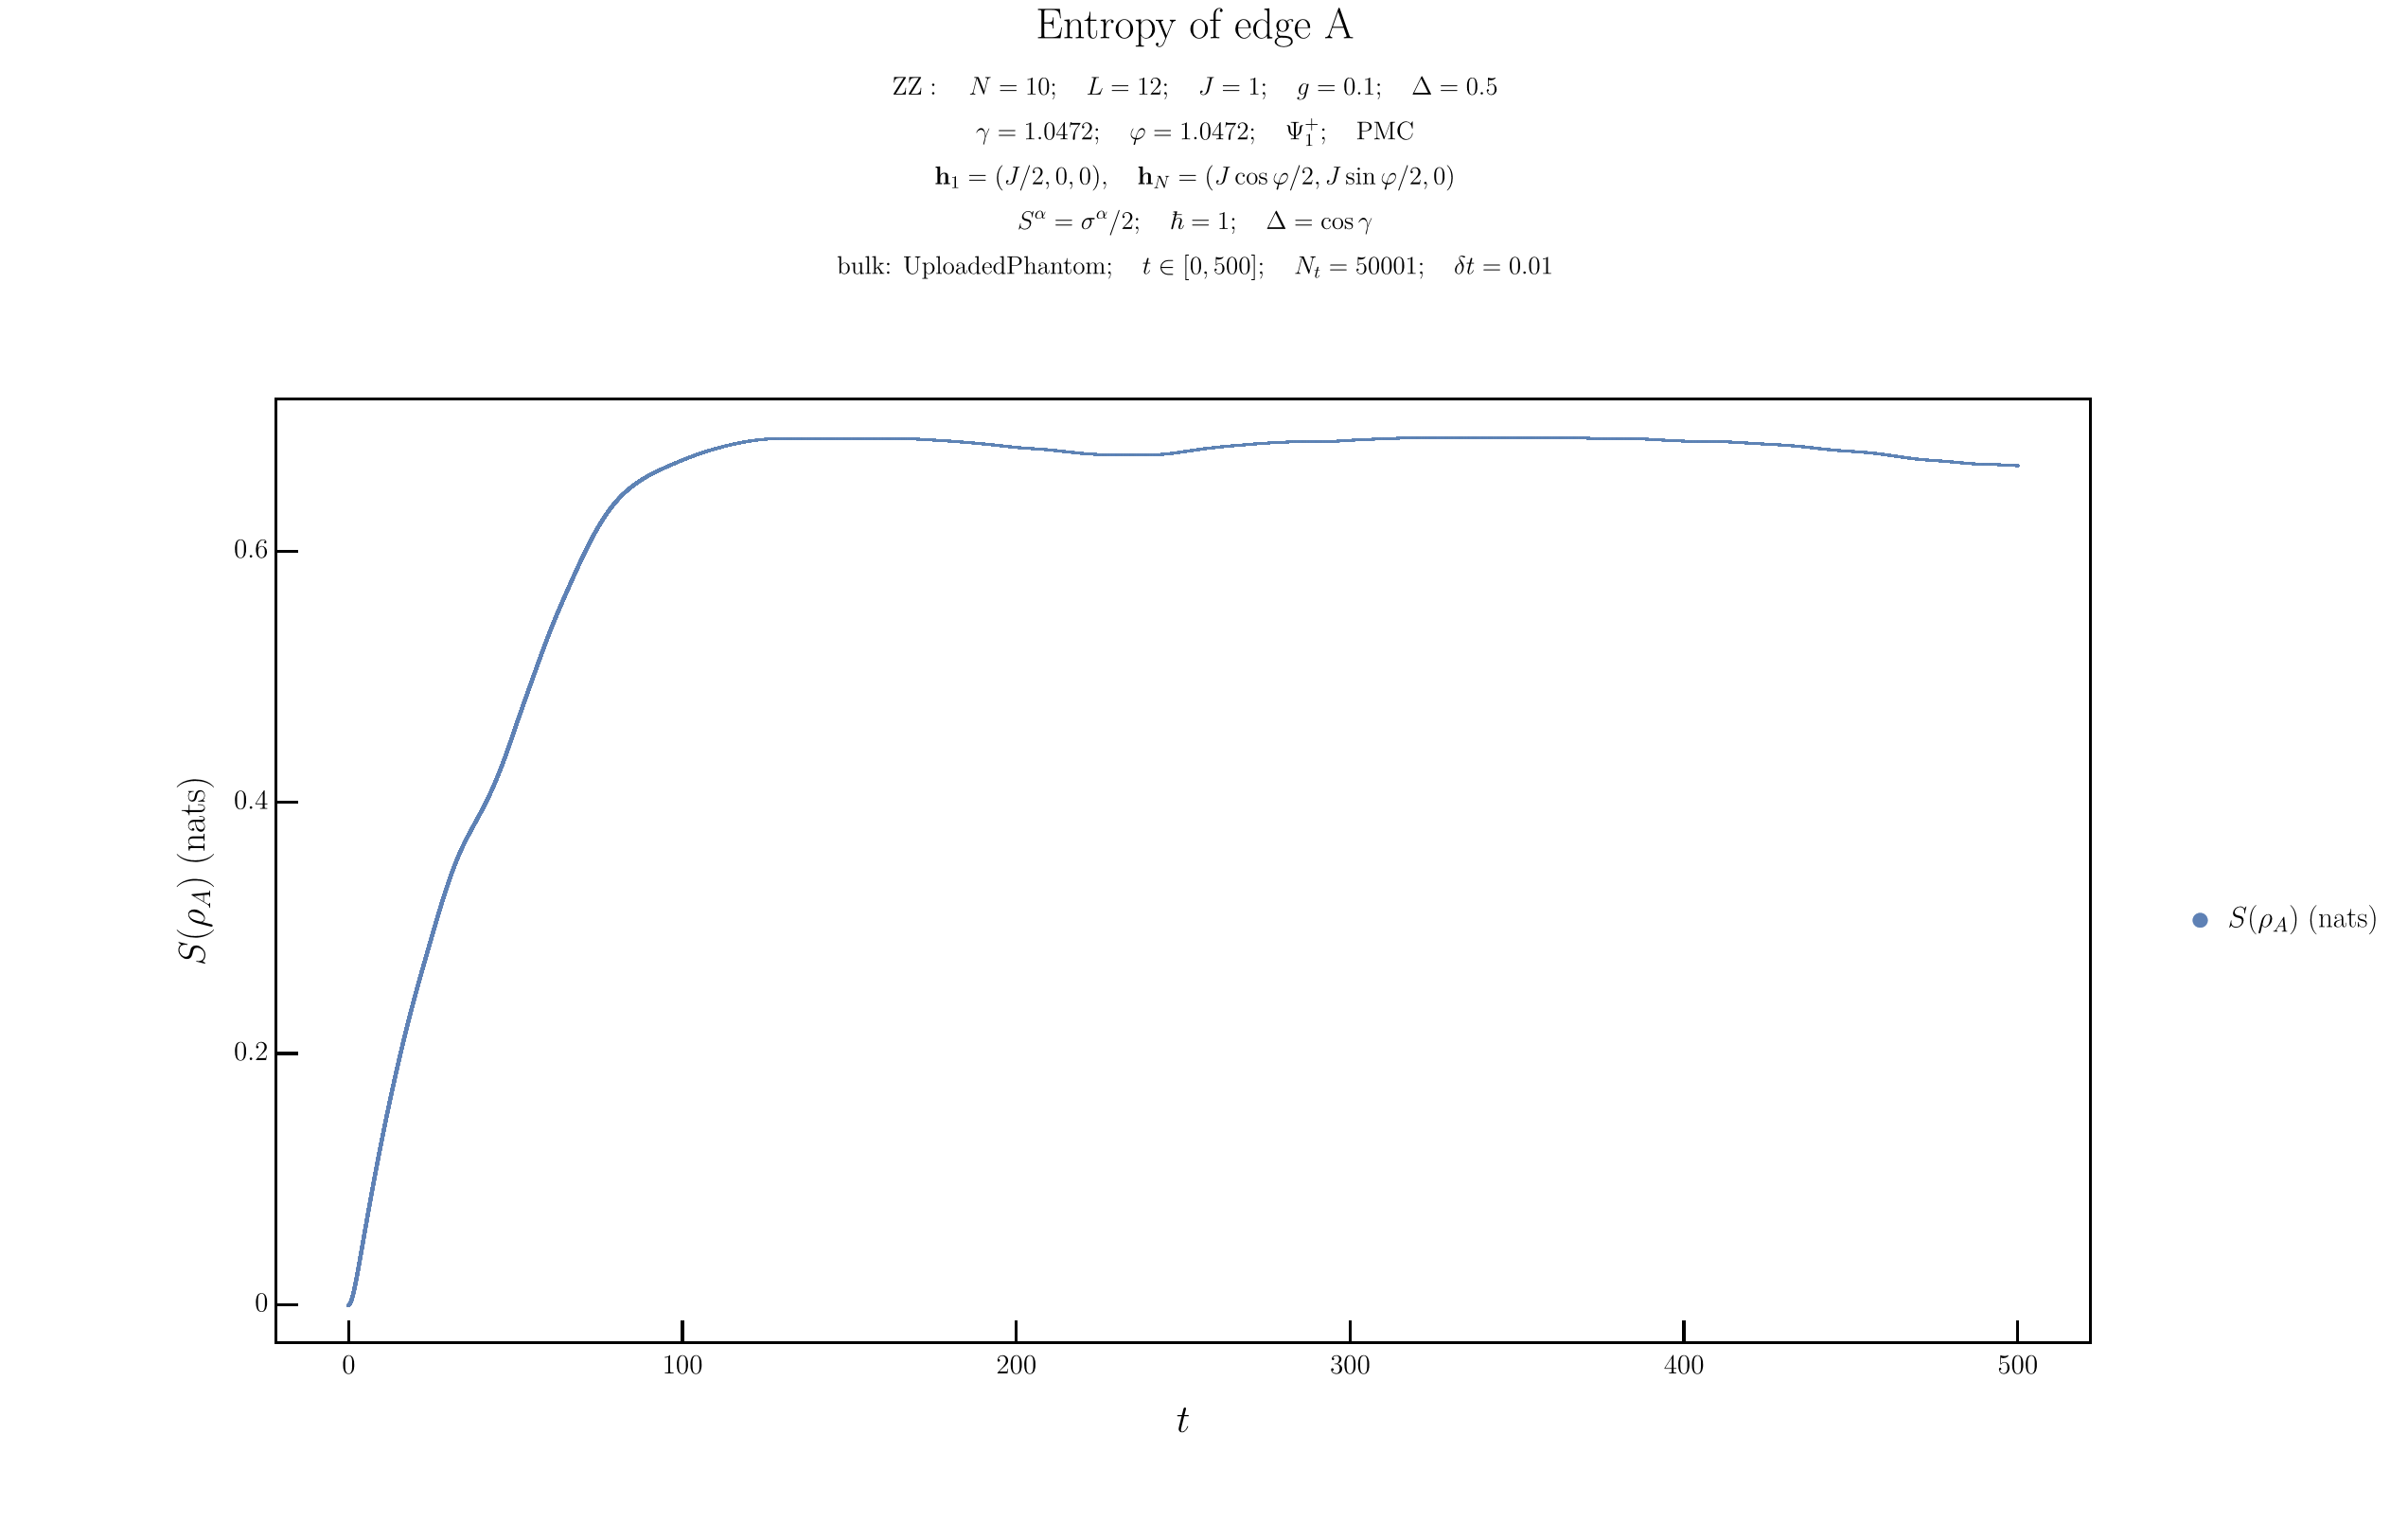
\includegraphics[width=\linewidth,height=0.39\textheight,keepaspectratio]{Phantom_ZZ_N10/State_EntropyA.png}
\end{column}
\begin{column}{0.41\textwidth}
\footnotesize
\[
S(\rho)=-\sum_{\lambda_k>0}\lambda_k\ln\lambda_k\equiv S(C_t/4)\text{ on }AB .
\]
\begin{itemize}\setlength\itemsep{5pt}
\item \textbf{Single-edge saturation:} $S(\rho_A)=S(\rho_B)$ reaches $0.689\approx\ln 2$ ($0.693$) by $t=125$ and stays within $[0.668,0.691]$ ($\Tr\rho_A^2\in[0.502,0.525]$).
\item \textbf{Two-edge recoherence dip:} $S(\rho_{AB})$ stays below $\ln 4\approx 1.386$ (max $1.285$ at $t=384.9$) and dips to \textbf{$0.887$} at $t=297.1$ where $\Tr\rho_{AB}^2$ peaks at $0.465$.
\item \textbf{Smoothness:} neither entropy shows any anomaly across $t=222.60$.
\end{itemize}
\end{column}
\end{columns}
\end{frame}

% ==============================================================
\begin{frame}{Bulk-mediated edge mutual information}
\begin{columns}[T,totalwidth=\textwidth]
\begin{column}{0.57\textwidth}
\centering
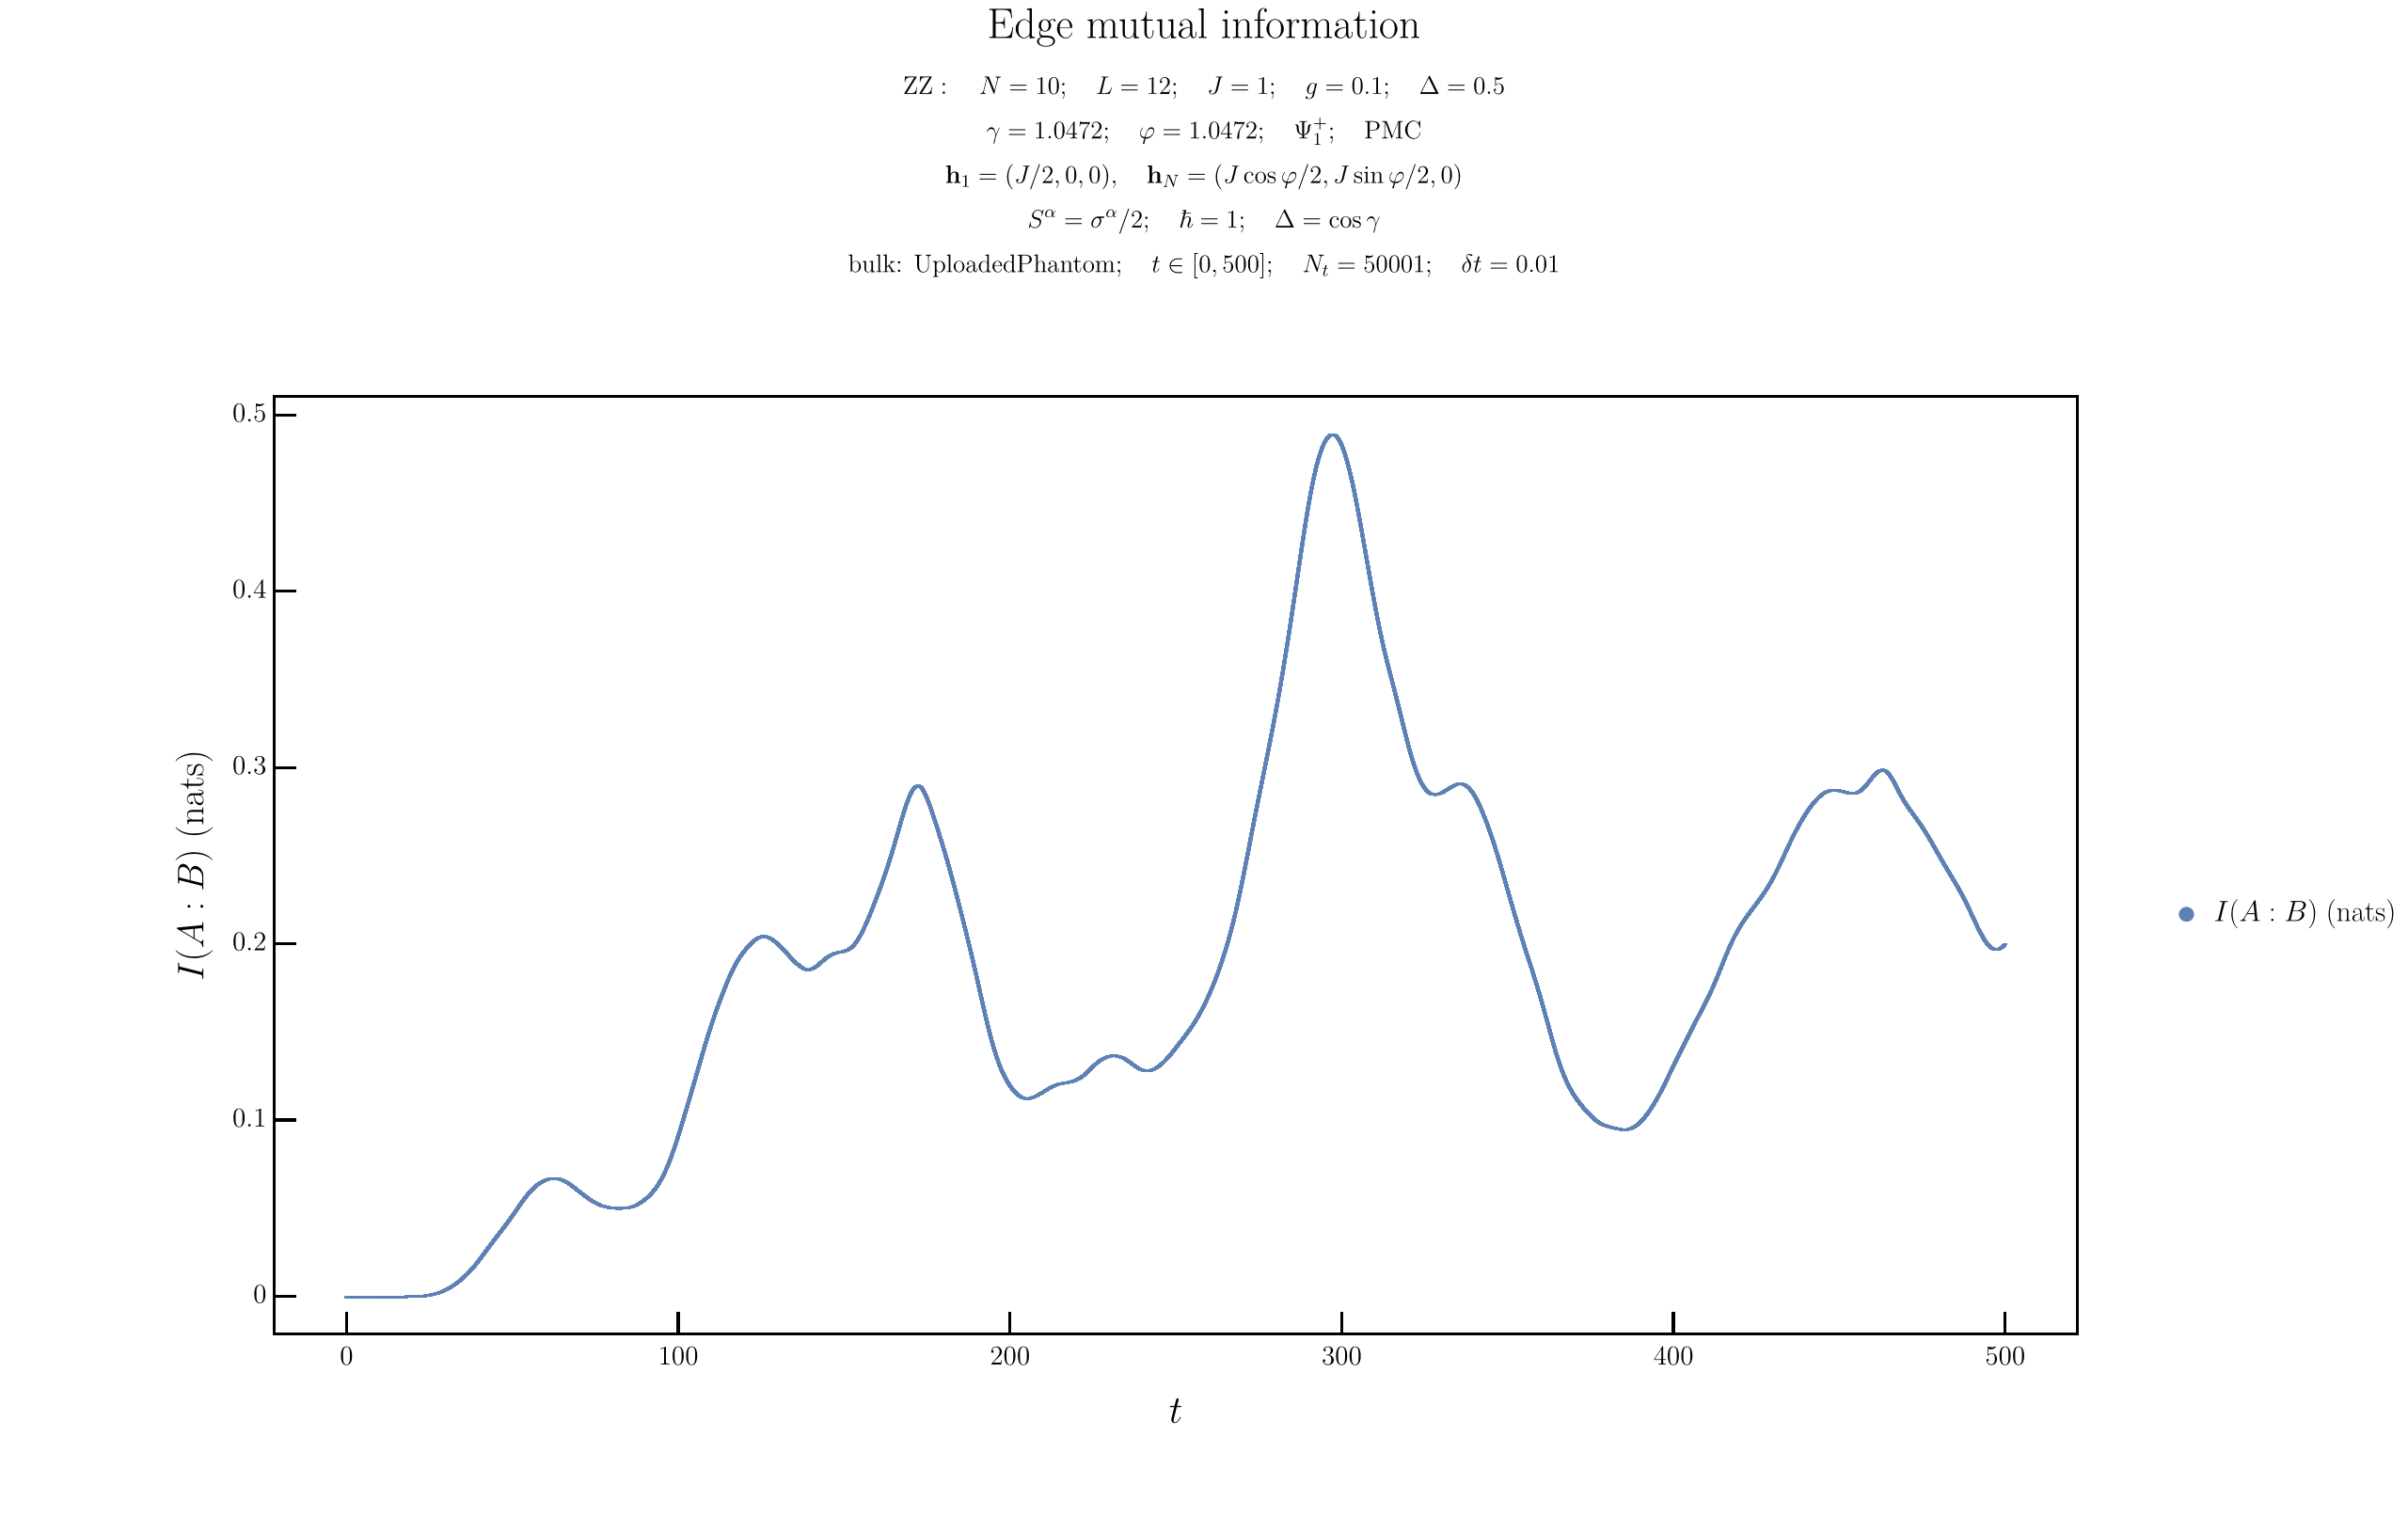
\includegraphics[width=\linewidth,height=0.77\textheight,keepaspectratio]{Phantom_ZZ_N10/State_MutualInfo.png}
\end{column}
\begin{column}{0.41\textwidth}
\footnotesize
\[
I(A:B)=S(\rho_A)+S(\rho_B)-S(\rho_{AB}).
\]
\begin{itemize}\setlength\itemsep{5pt}
\item \textbf{Causal onset ($t\lesssim 20$):} $I(A:B)\approx 0$ until bulk excitations traverse the $N=10$ chain and break the short-time factorization $\Gamma(t)\approx\gamma_A(t)\otimes\gamma_B(t)$.
\item \textbf{Strong mediated correlations:} without direct $A$--$B$ coupling, $I(A:B)$ peaks at $t=172.3$ ($0.290$), \textbf{$t=297.3$ ($0.489$~nats)}, and $t=463.0$ ($0.299$).
\item \textbf{Smooth through $t=222.60$:} passes smoothly near $I(A:B)\approx 0.13$ during the canonical-rate spike.
\end{itemize}
\end{column}
\end{columns}
\end{frame}

% ==============================================================
\begin{frame}{Two-point Pauli correlations between the edges}
\footnotesize
\begin{columns}[T,totalwidth=\textwidth]
\begin{column}{0.49\textwidth}
\centering
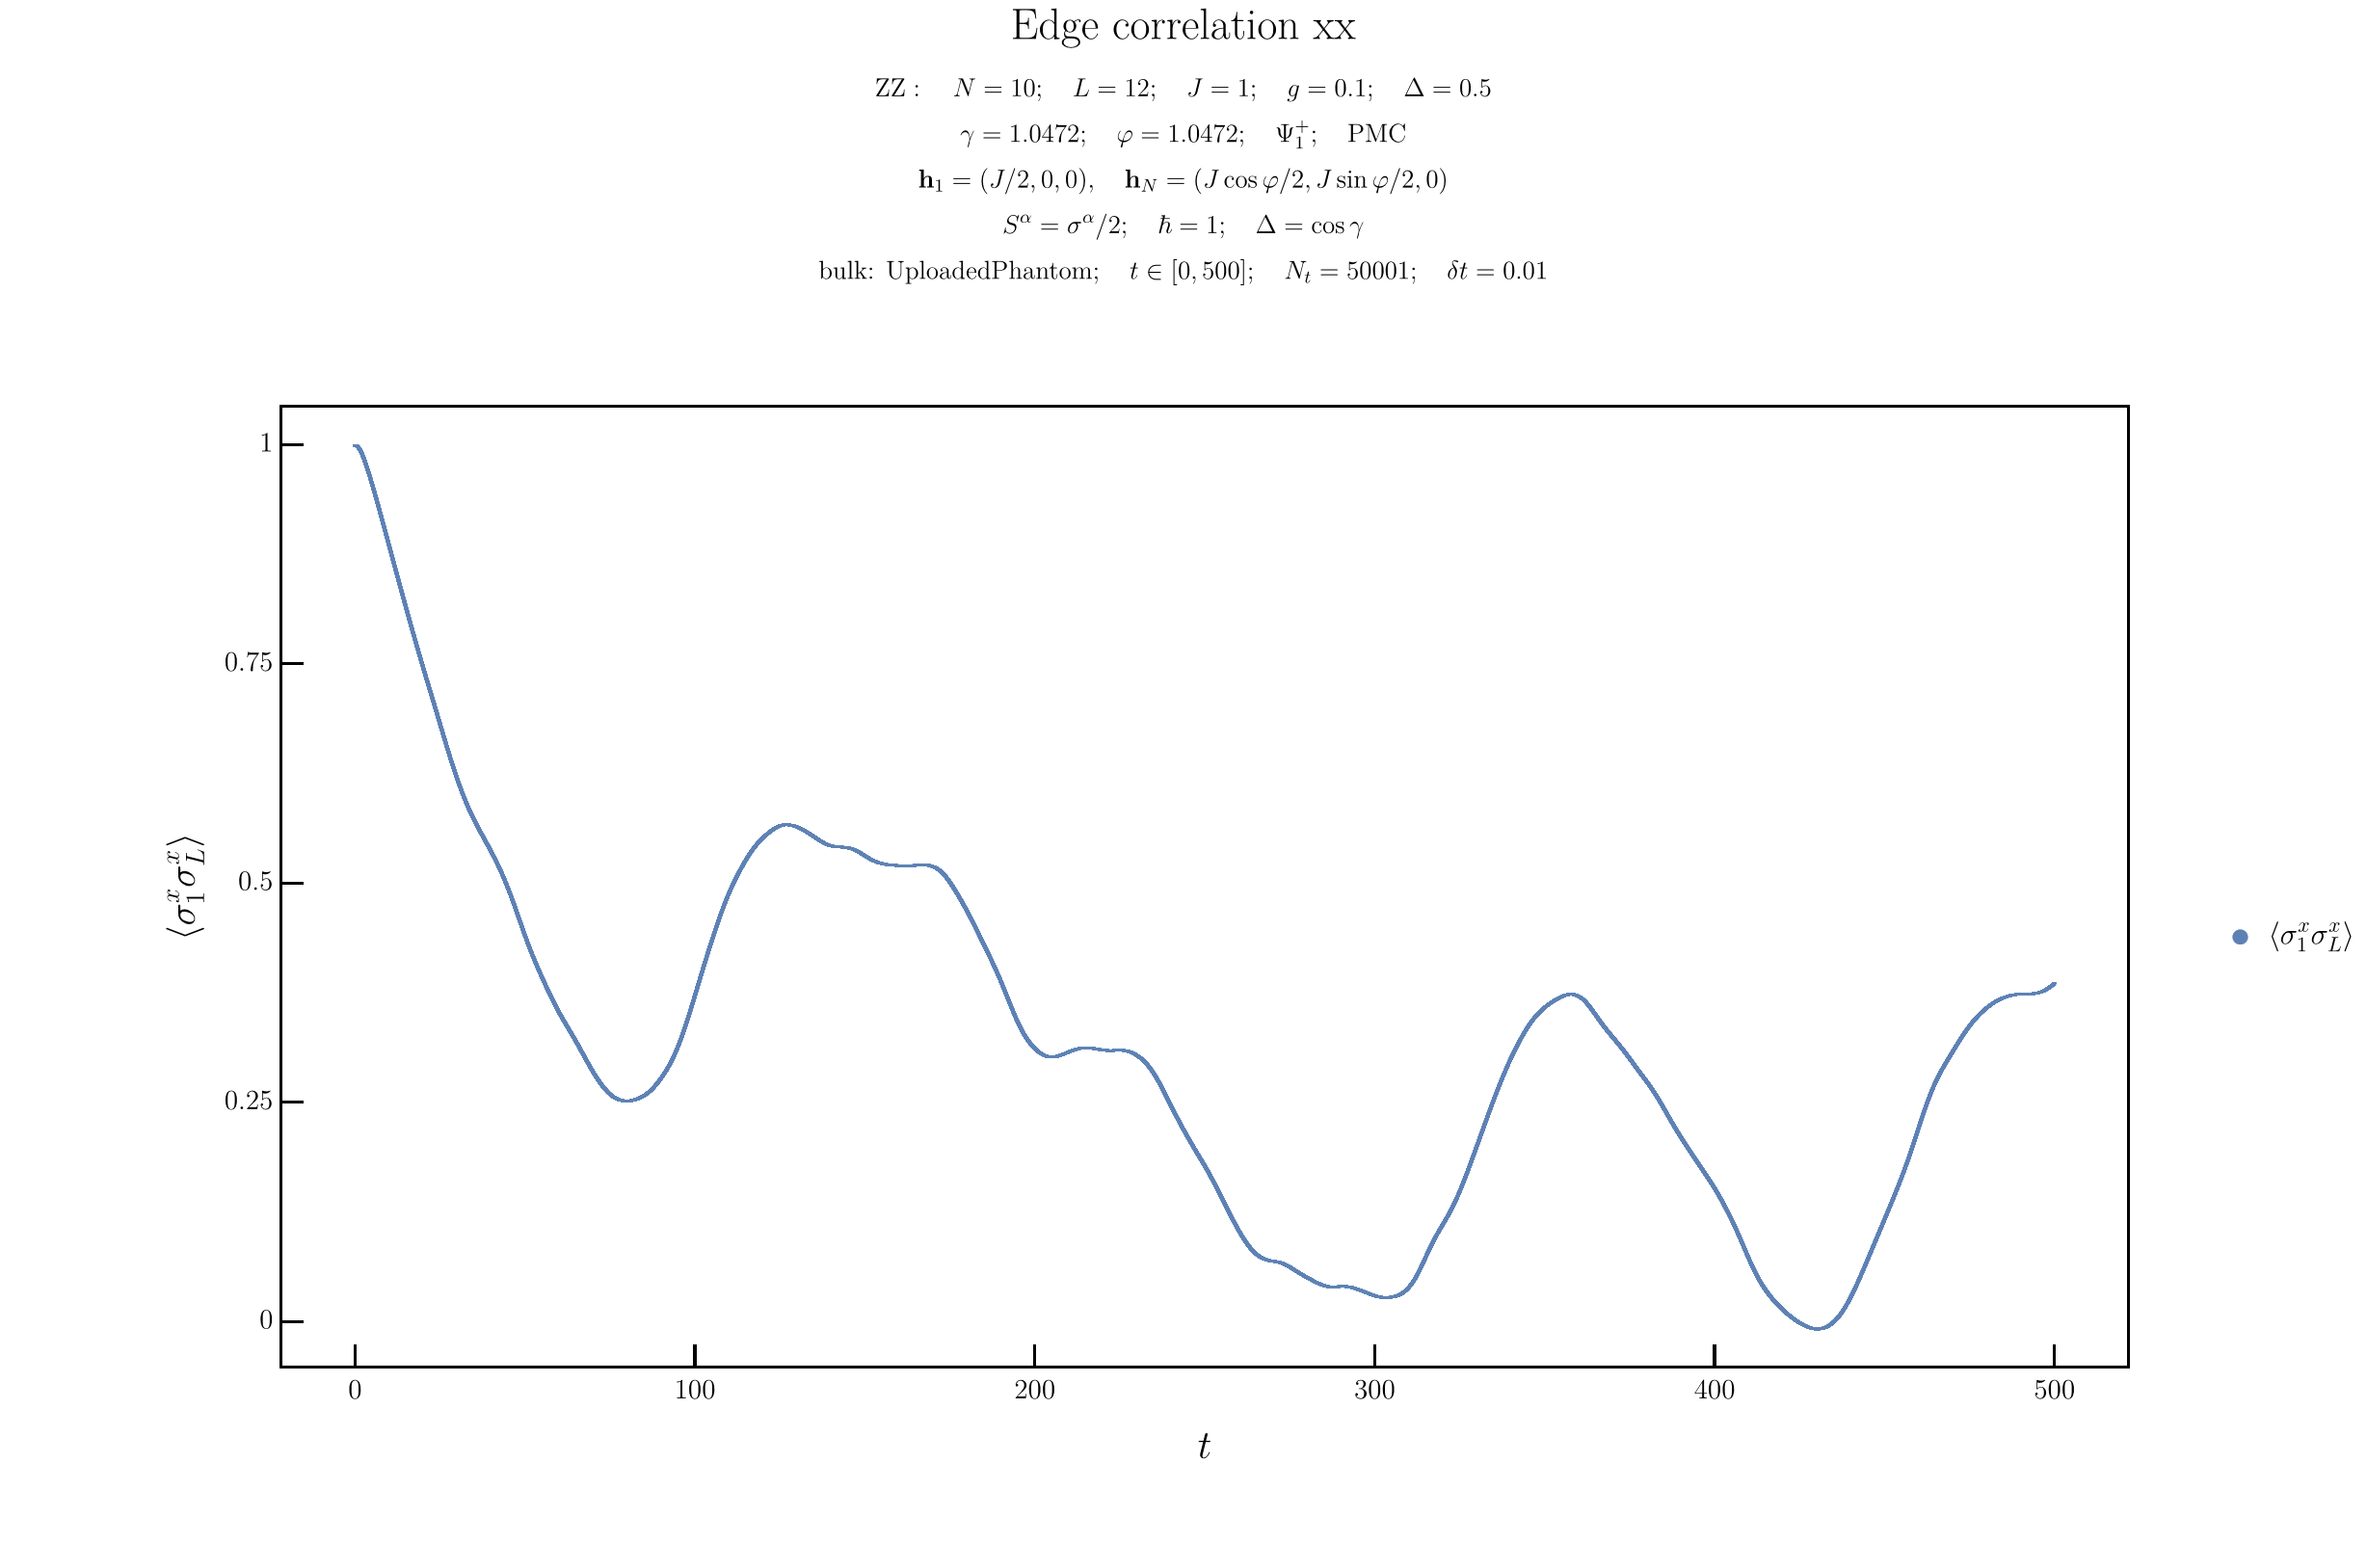
\includegraphics[width=\linewidth,height=0.49\textheight,keepaspectratio]{Phantom_ZZ_N10/State_CorrelationXX.png}
\end{column}
\begin{column}{0.49\textwidth}
\centering
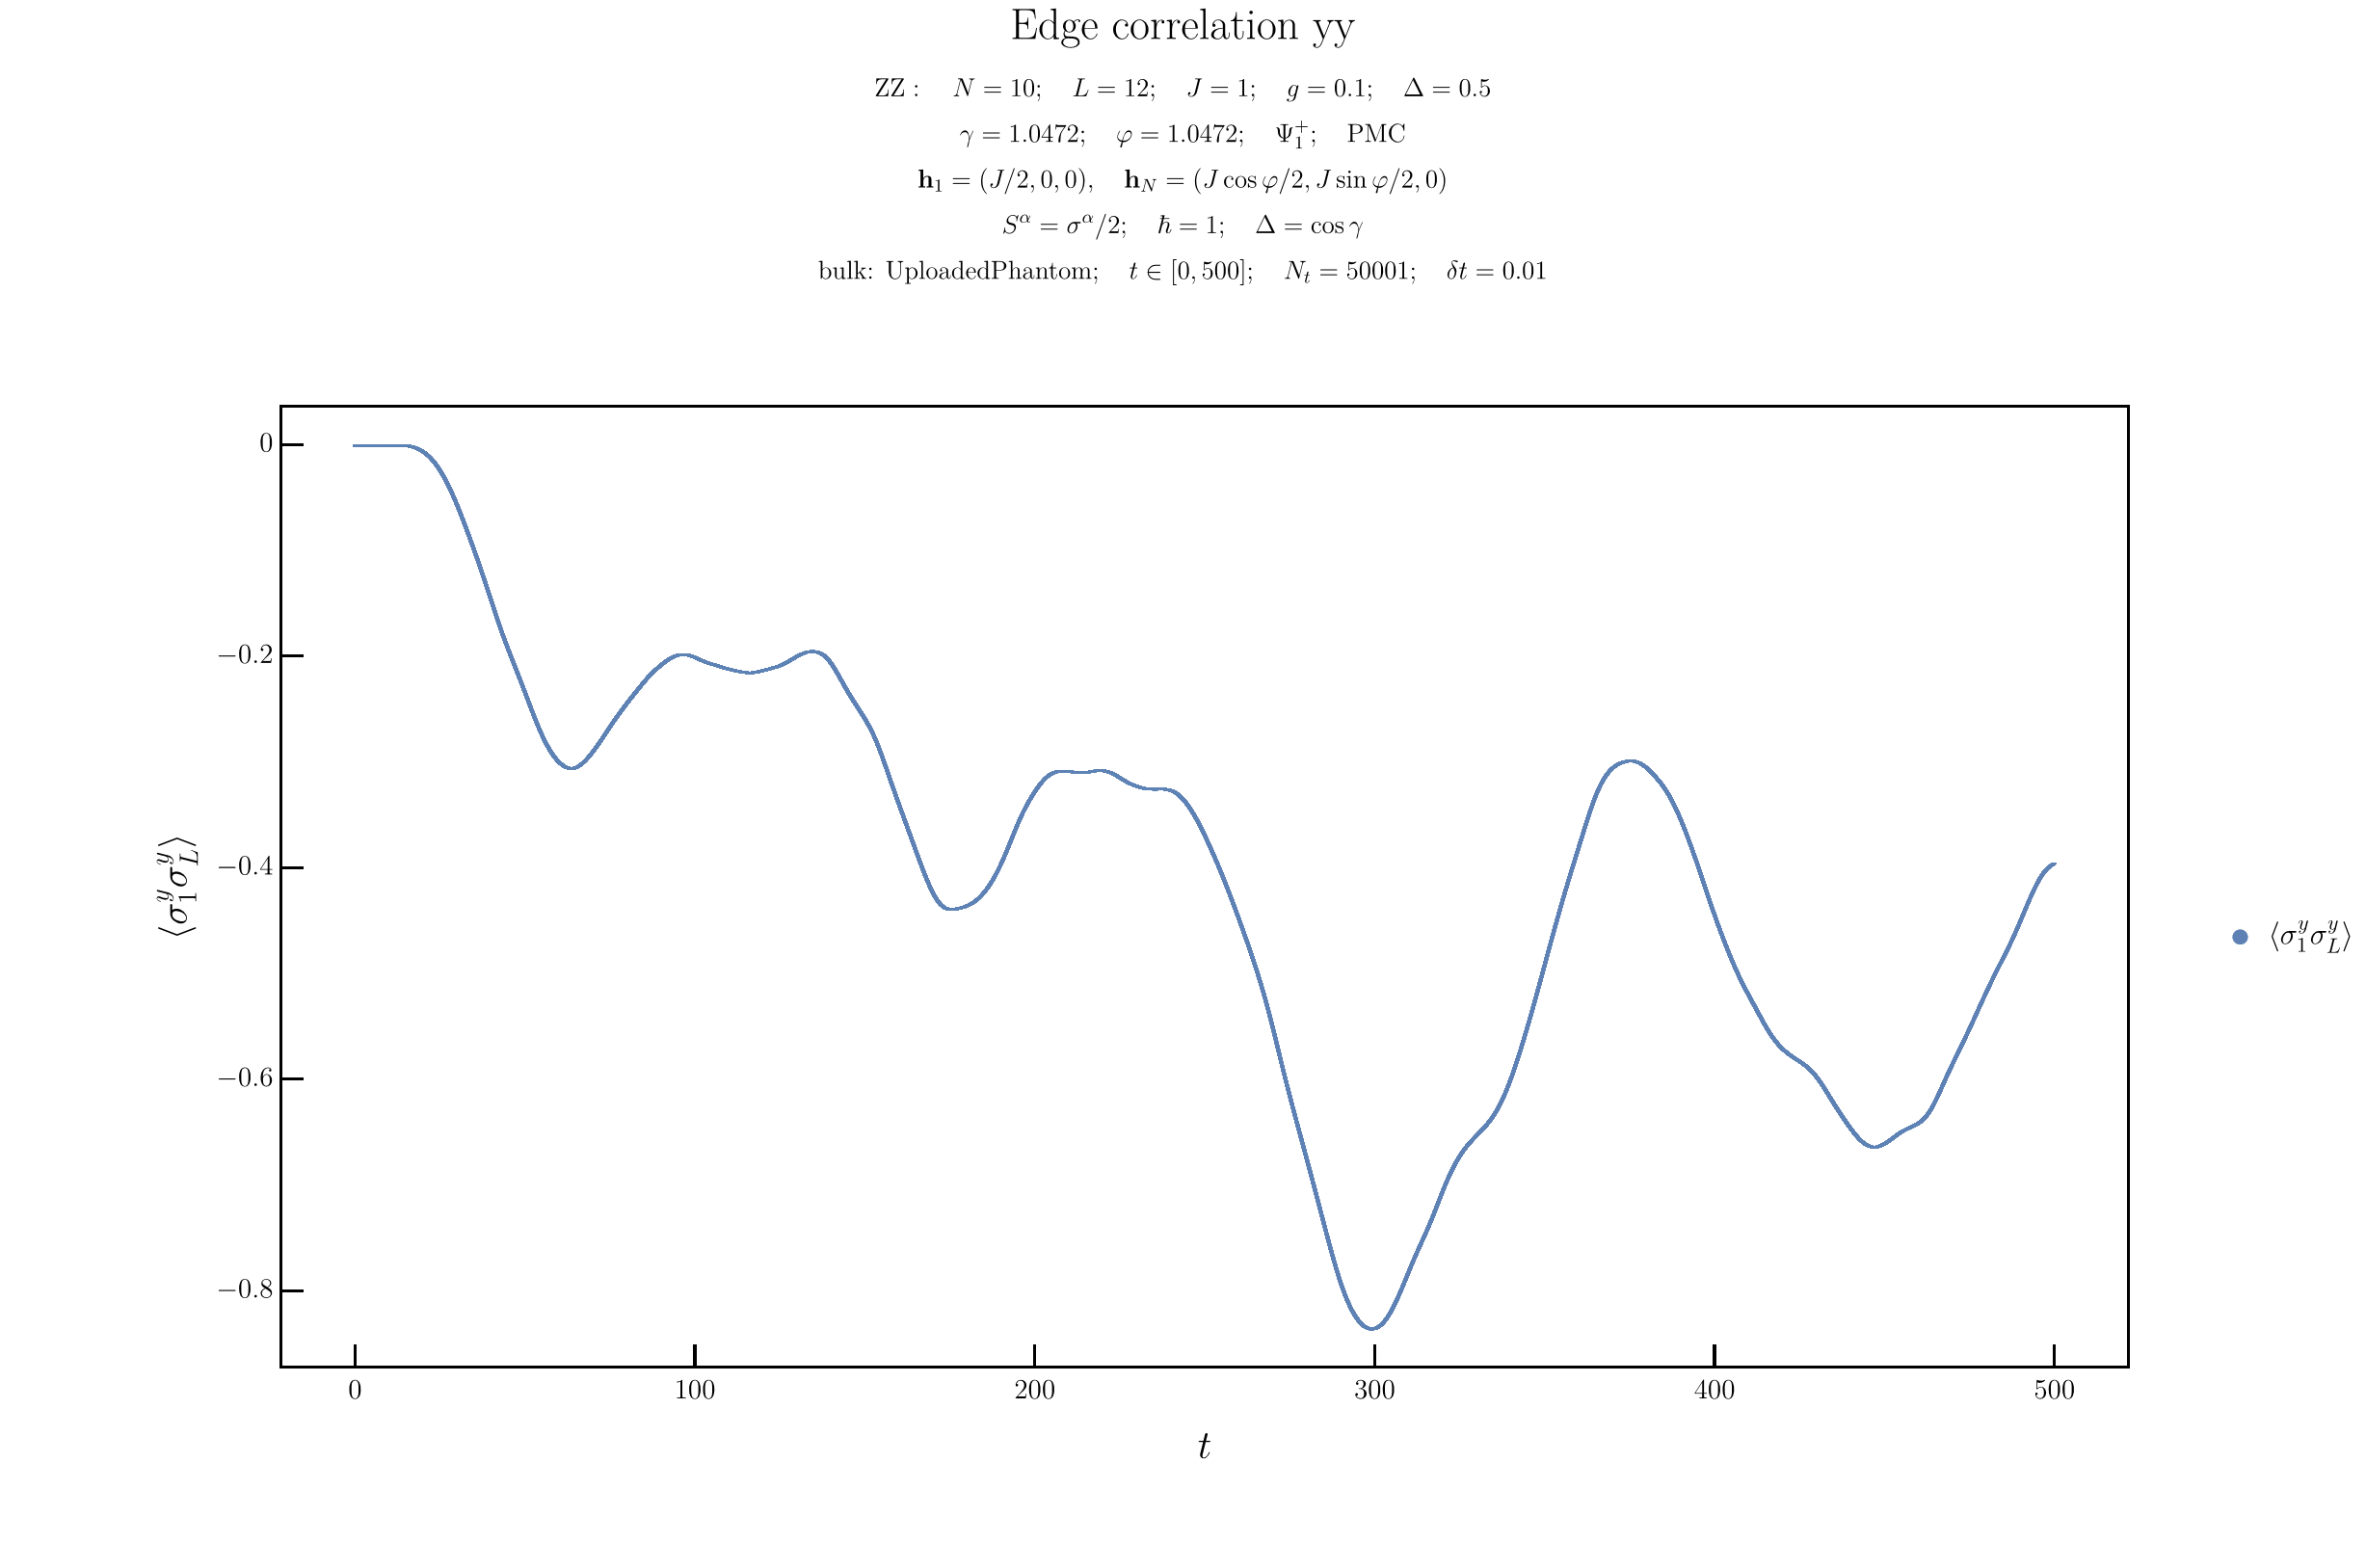
\includegraphics[width=\linewidth,height=0.49\textheight,keepaspectratio]{Phantom_ZZ_N10/State_CorrelationYY.png}
\end{column}
\end{columns}
\vspace{-4pt}
\[
C_{\alpha\beta}(t)=\Tr\!\bigl[(\sigma_A^\alpha\otimes\sigma_B^\beta)\,\rho_{AB}(t)\bigr],\qquad
C_{\alpha\beta}^c(t)=C_{\alpha\beta}(t)-\langle\sigma_A^\alpha\rangle\langle\sigma_B^\beta\rangle .
\]
\vspace{-6pt}
\begin{itemize}\setlength\itemsep{2pt}
\item \textbf{Transverse pair:} $C_{yy}=\tfrac12\operatorname{Re}(\Gamma_{01,10}-\Gamma_{00,11})$ plunges to \textbf{$-0.836$} at $t=299.2$, while $C_{xx}=\tfrac12\operatorname{Re}(\Gamma_{01,10}+\Gamma_{00,11})$ drops from $1$ to $0.03$ there ($\sigma_1,\sigma_L\equiv\sigma_A,\sigma_B$).
\item \textbf{Exact $\mathcal R\mathcal F$ identities:} $C_{zx}=-C_{xz}$, $C_{zy}=C_{yz}$, and $C_{yx}=-C_{xy}$ (and $C_{yx}^c=-C_{xy}^c$) hold to $5.7\times 10^{-14}$.
\item \textbf{Nonzero mixed $z$-correlations:} $C_{xz}\in[-0.063,0.180]$ and $C_{yz}\in[-0.244,0.097]$ ($C_{\alpha z}^c=C_{\alpha z}$ since $\langle\sigma^z\rangle=0$; Appendix~2d).
\end{itemize}
\end{frame}

% ==============================================================
\begin{frame}{Entanglement between the edges}
\begin{columns}[T,totalwidth=\textwidth]
\begin{column}{0.57\textwidth}
\centering
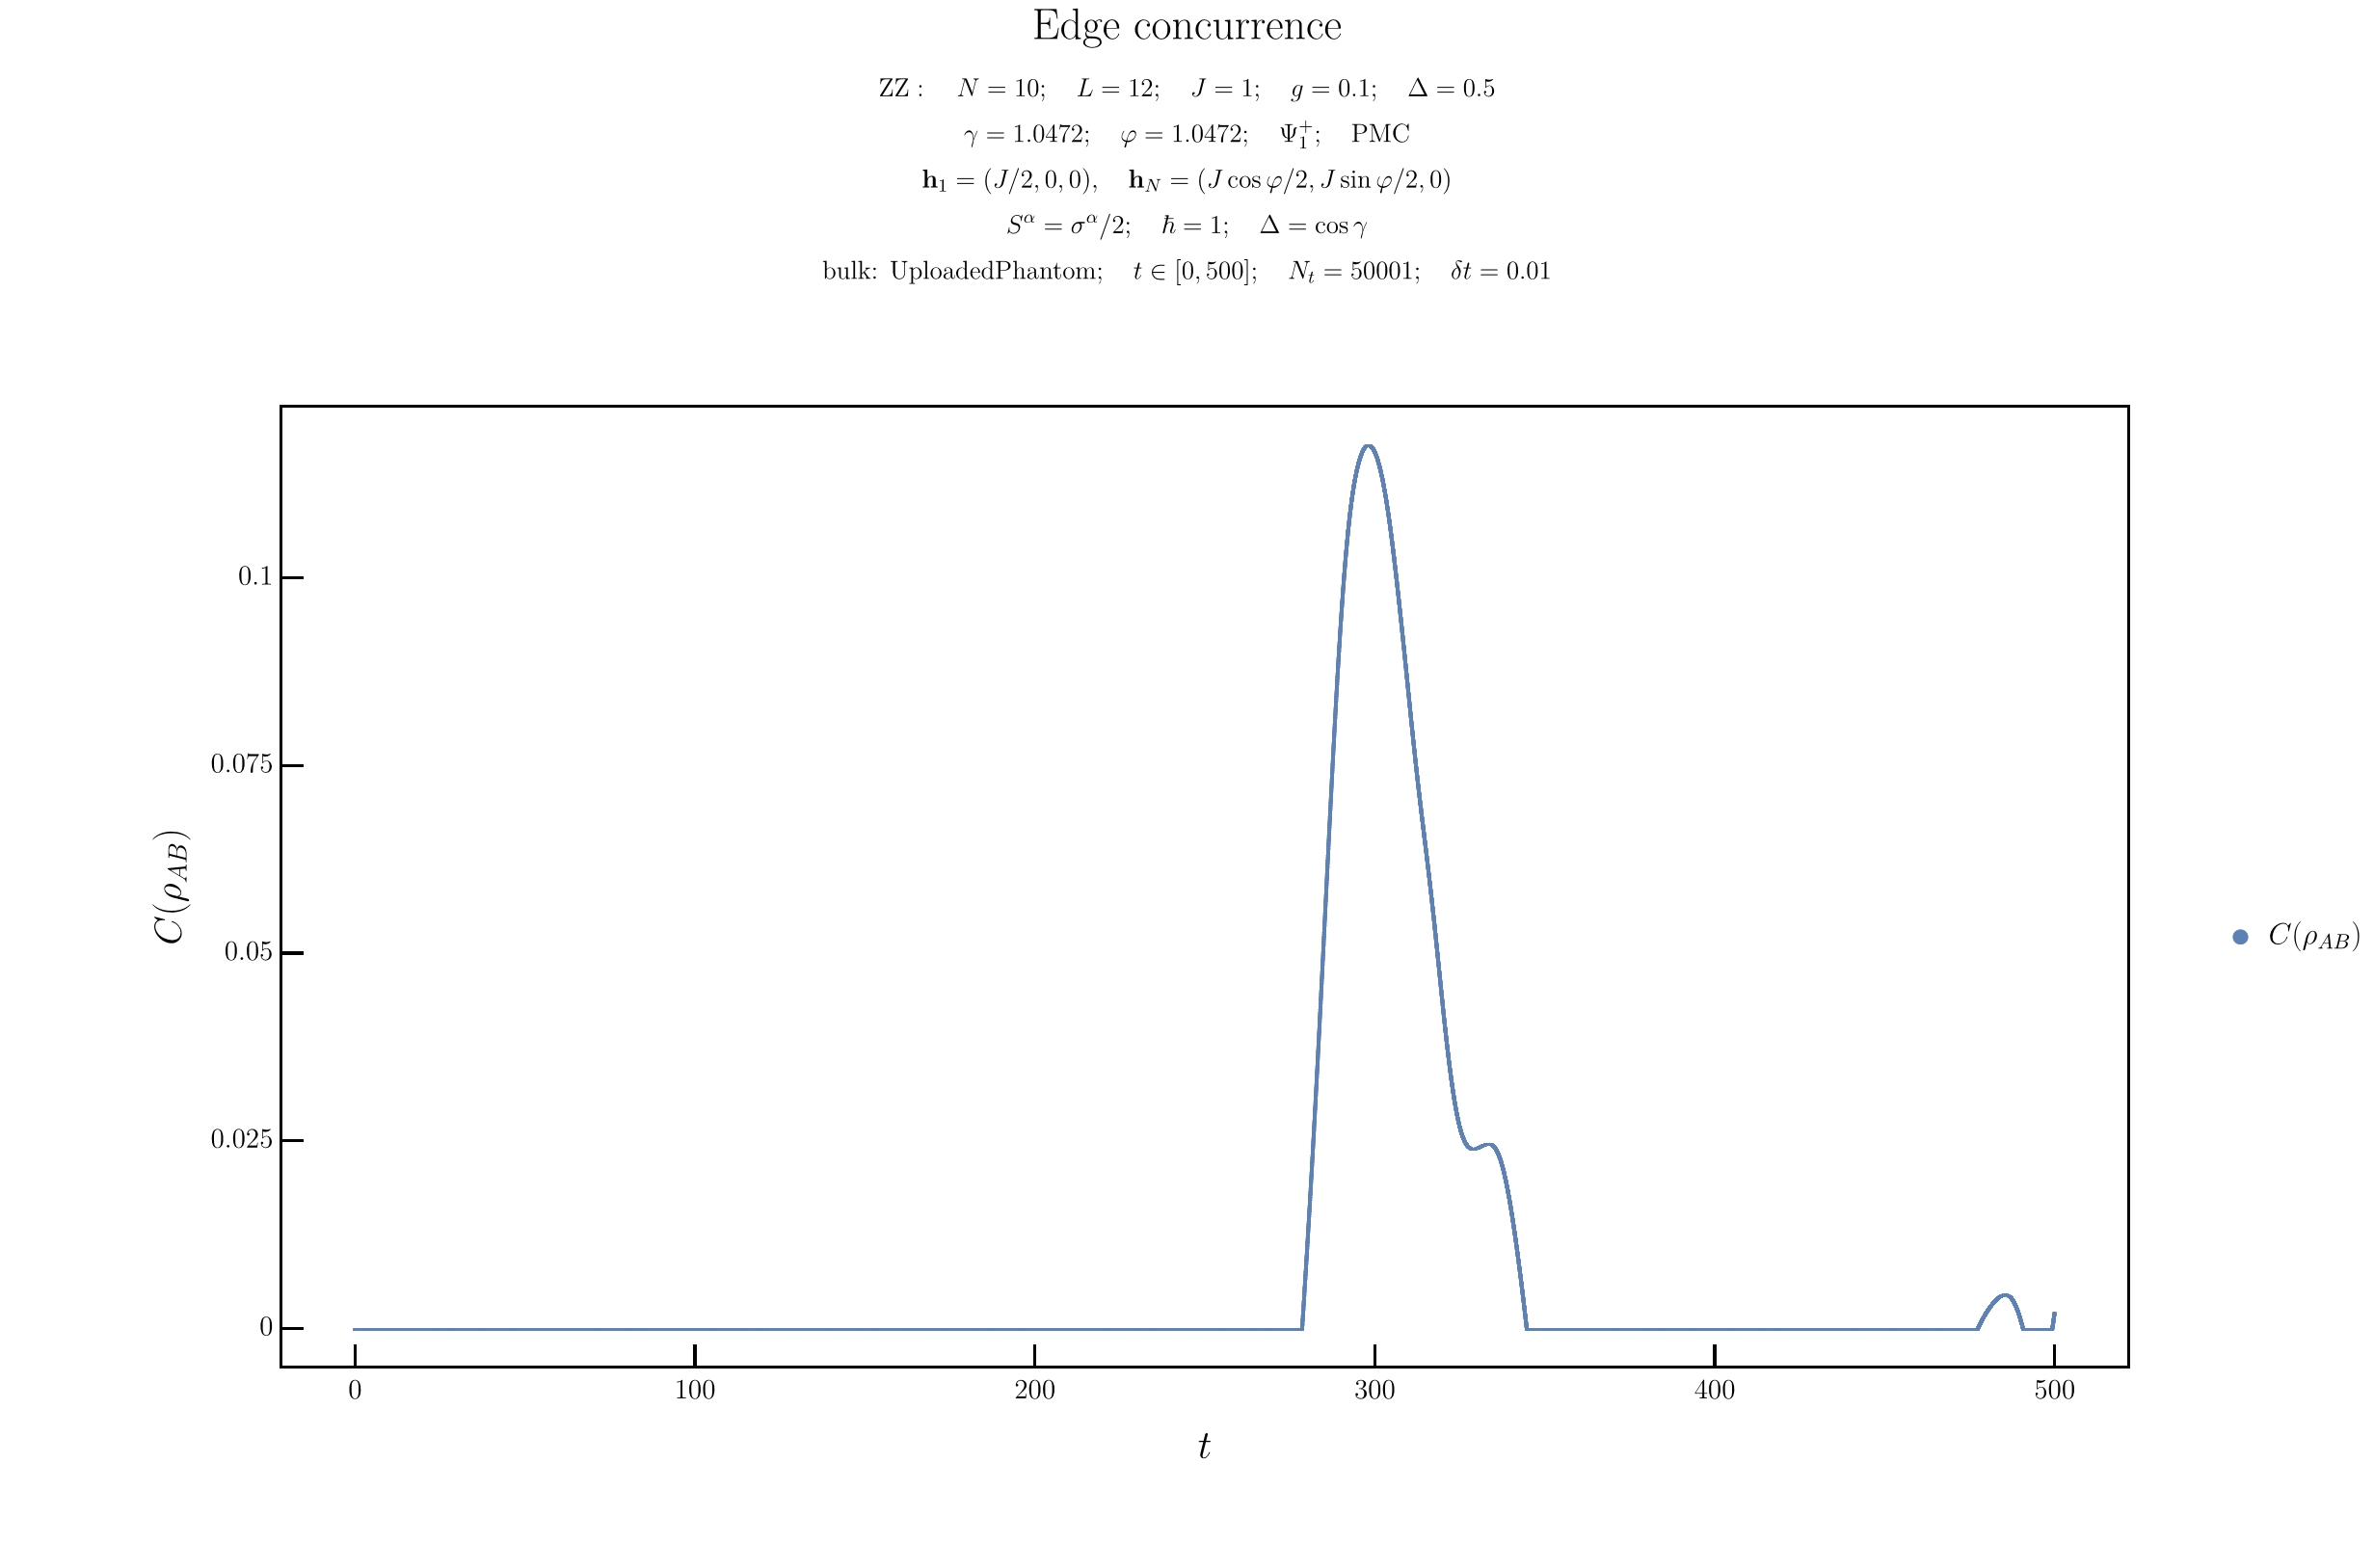
\includegraphics[width=\linewidth,height=0.77\textheight,keepaspectratio]{Phantom_ZZ_N10/State_Concurrence.png}
\end{column}
\begin{column}{0.41\textwidth}
\footnotesize\setlength\abovedisplayskip{3pt}\setlength\belowdisplayskip{3pt}
\[
C(\rho_{AB})=C\bigl[\Gamma(t)/4\bigr]=\max_{\rho\in\mathrm{Sep}}C\bigl[\Lambda_t(\rho)\bigr].
\]
\begin{itemize}\setlength\itemsep{2.5pt}
\item \textbf{Entanglement window \cite{Wootters1998}:} $C(\rho_{AB})\equiv 0$ until $t=278.64$, peaks at \textbf{$0.118$} at $t=298.16$, and returns to $0$ at $t=344.72$ (minor revivals $0.0045$ on $[477.4,490.7]$ and $0.0021$ at $500$).
\item \textbf{Mechanism:} driven by the sign flip $\operatorname{Re}\Gamma_{01,10}=-0.805$ alongside high $\Gamma_{00,11}\approx 0.87$; negativity matches in shape (peak $0.0587$, Appendix~2b).
\item \textbf{Separable-input capacity:} $\ket{++}$ attains the channel maximum over all separable inputs; $C\ll 1$ (no Bell state, consistent with the Schur no-go).
\end{itemize}
\end{column}
\end{columns}
\end{frame}

% ==============================================================
\begin{frame}{Return probabilities and bulk Loschmidt echo}
\begin{columns}[T,totalwidth=\textwidth]
\begin{column}{0.57\textwidth}
\centering
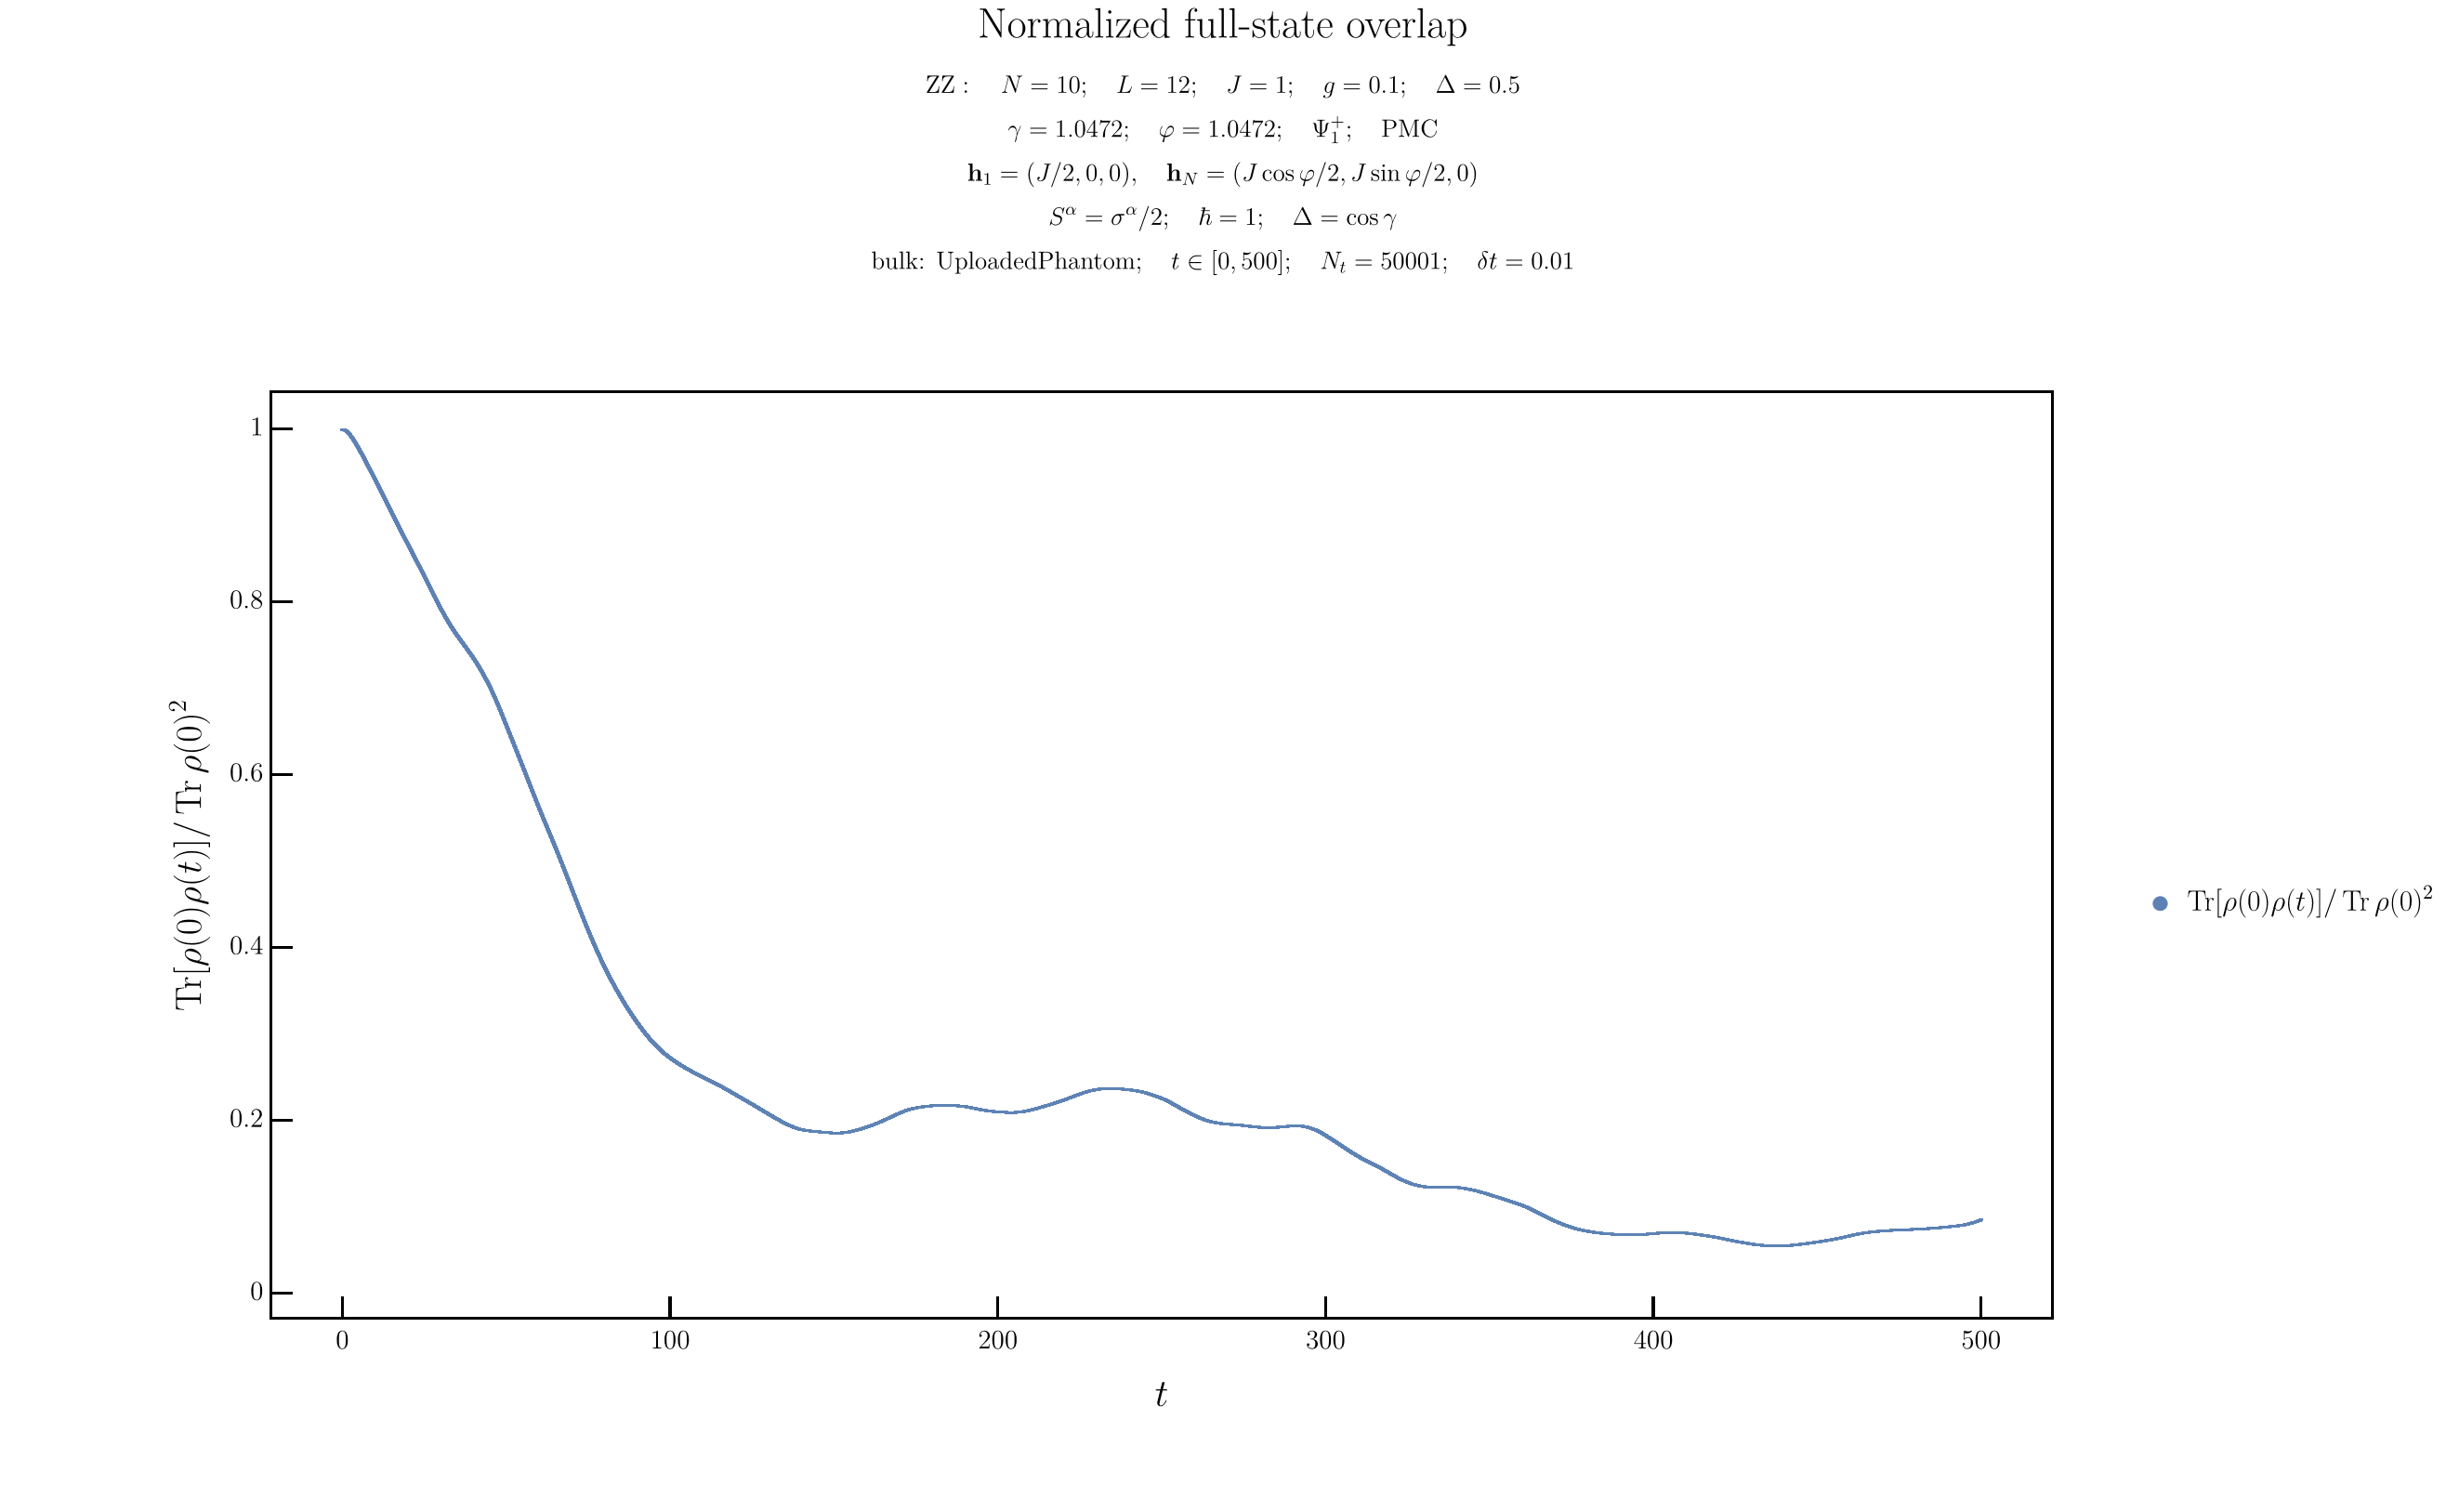
\includegraphics[width=\linewidth,height=0.41\textheight,keepaspectratio]{Phantom_ZZ_N10/State_FullOverlap.png}\\[2pt]
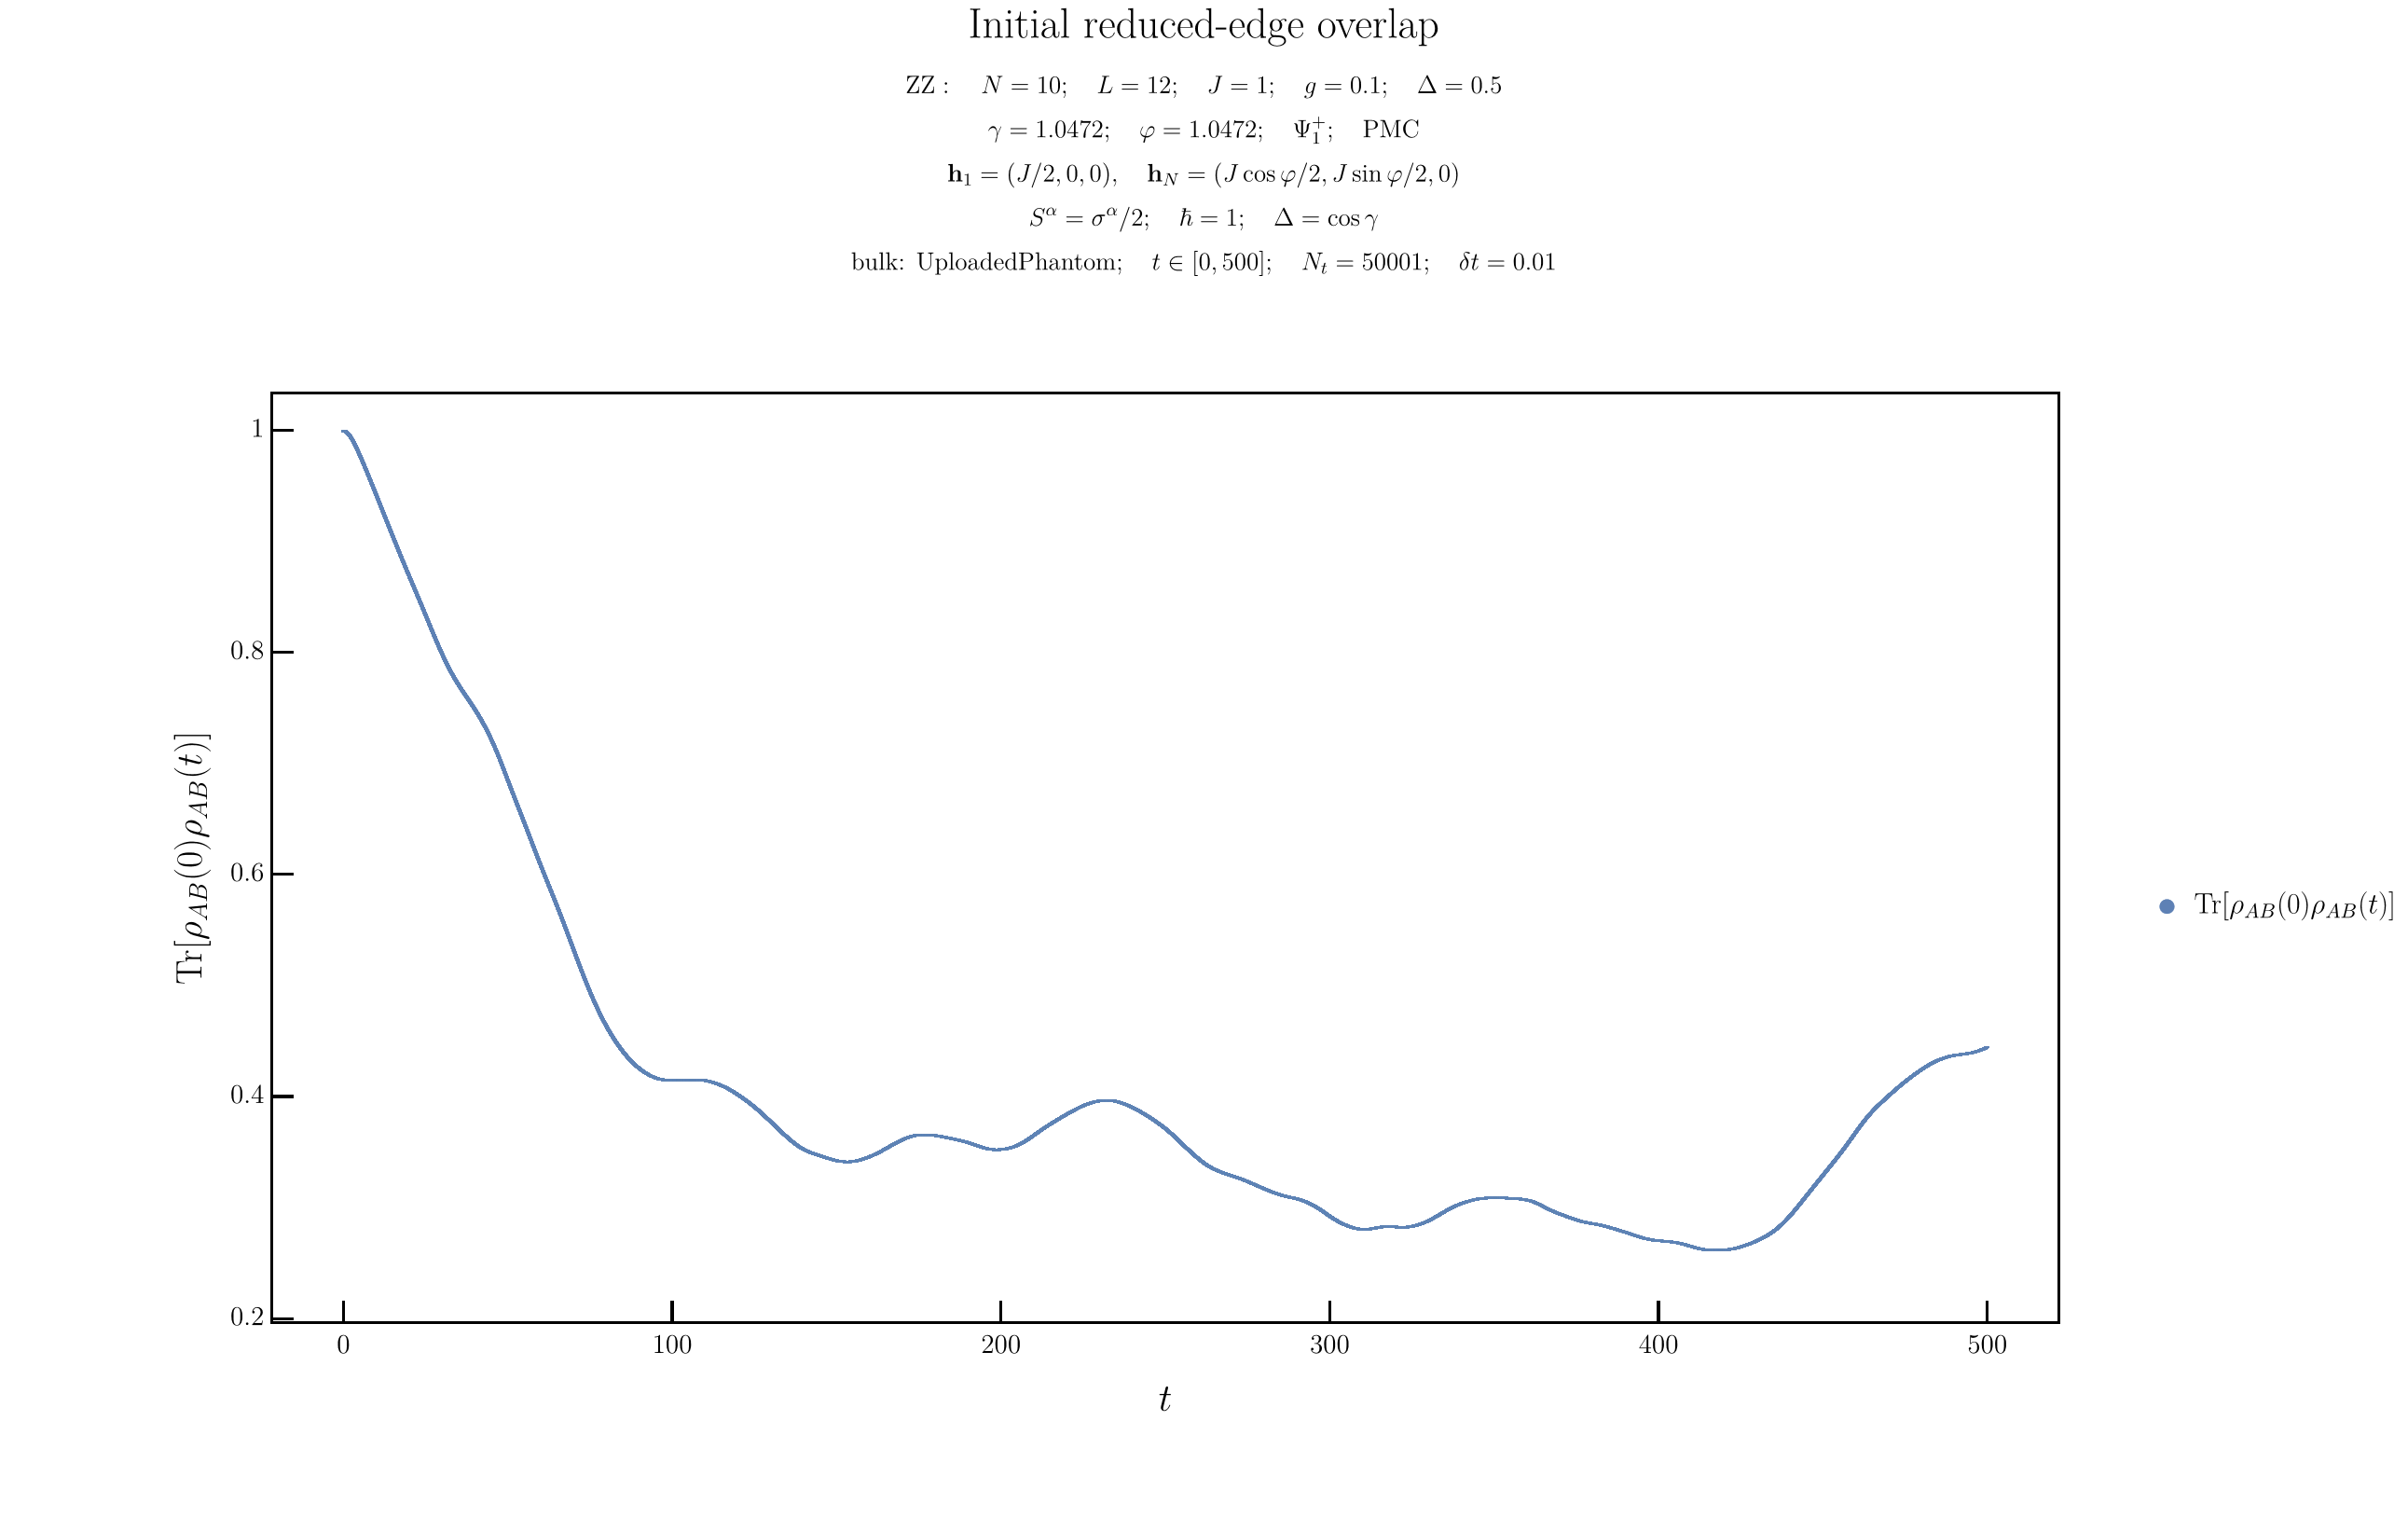
\includegraphics[width=\linewidth,height=0.39\textheight,keepaspectratio]{Phantom_ZZ_N10/State_InitialOverlap.png}
\end{column}
\begin{column}{0.41\textwidth}
\footnotesize
\[
\mathcal F_{\mathrm{full}}(t)
=\tfrac{1}{16}\Bigl\lvert\textstyle\sum_a\langle\psi_M\vert\phi_a(t)\rangle\Bigr\rvert^2 .
\]
\begin{itemize}\setlength\itemsep{4pt}
\item \textbf{Global survival (top):} $\lvert\langle\Psi(0)\vert\Psi(t)\rangle\rvert^2$ is a 4-branch Loschmidt echo of $\ket{\psi_M}$ (verified to $3.8\times 10^{-14}$), falling to $0.055$ at $t=437.7$ ($0.085$ at $t=500$).
\item \textbf{Reduced-edge overlap (bottom):} $\Tr[\rho_{AB}(0)\rho_{AB}(t)]=\tfrac{1}{16}\sum_{a,b}\Gamma_{ab}(t)$ drops to $0.415$ by $t=100$ and $0.262$ at $t=417.6$, reviving to $0.445$ at $t=500$ (axis starts at $0.2$).
\item \textbf{Smoothness:} both overlaps are smooth across $t=222.60$.
\end{itemize}
\end{column}
\end{columns}
\end{frame}

% ==============================================================
\begin{frame}{Choi spectrum and sorting kinks}
\begin{columns}[T,totalwidth=\textwidth]
\begin{column}{0.57\textwidth}
\centering
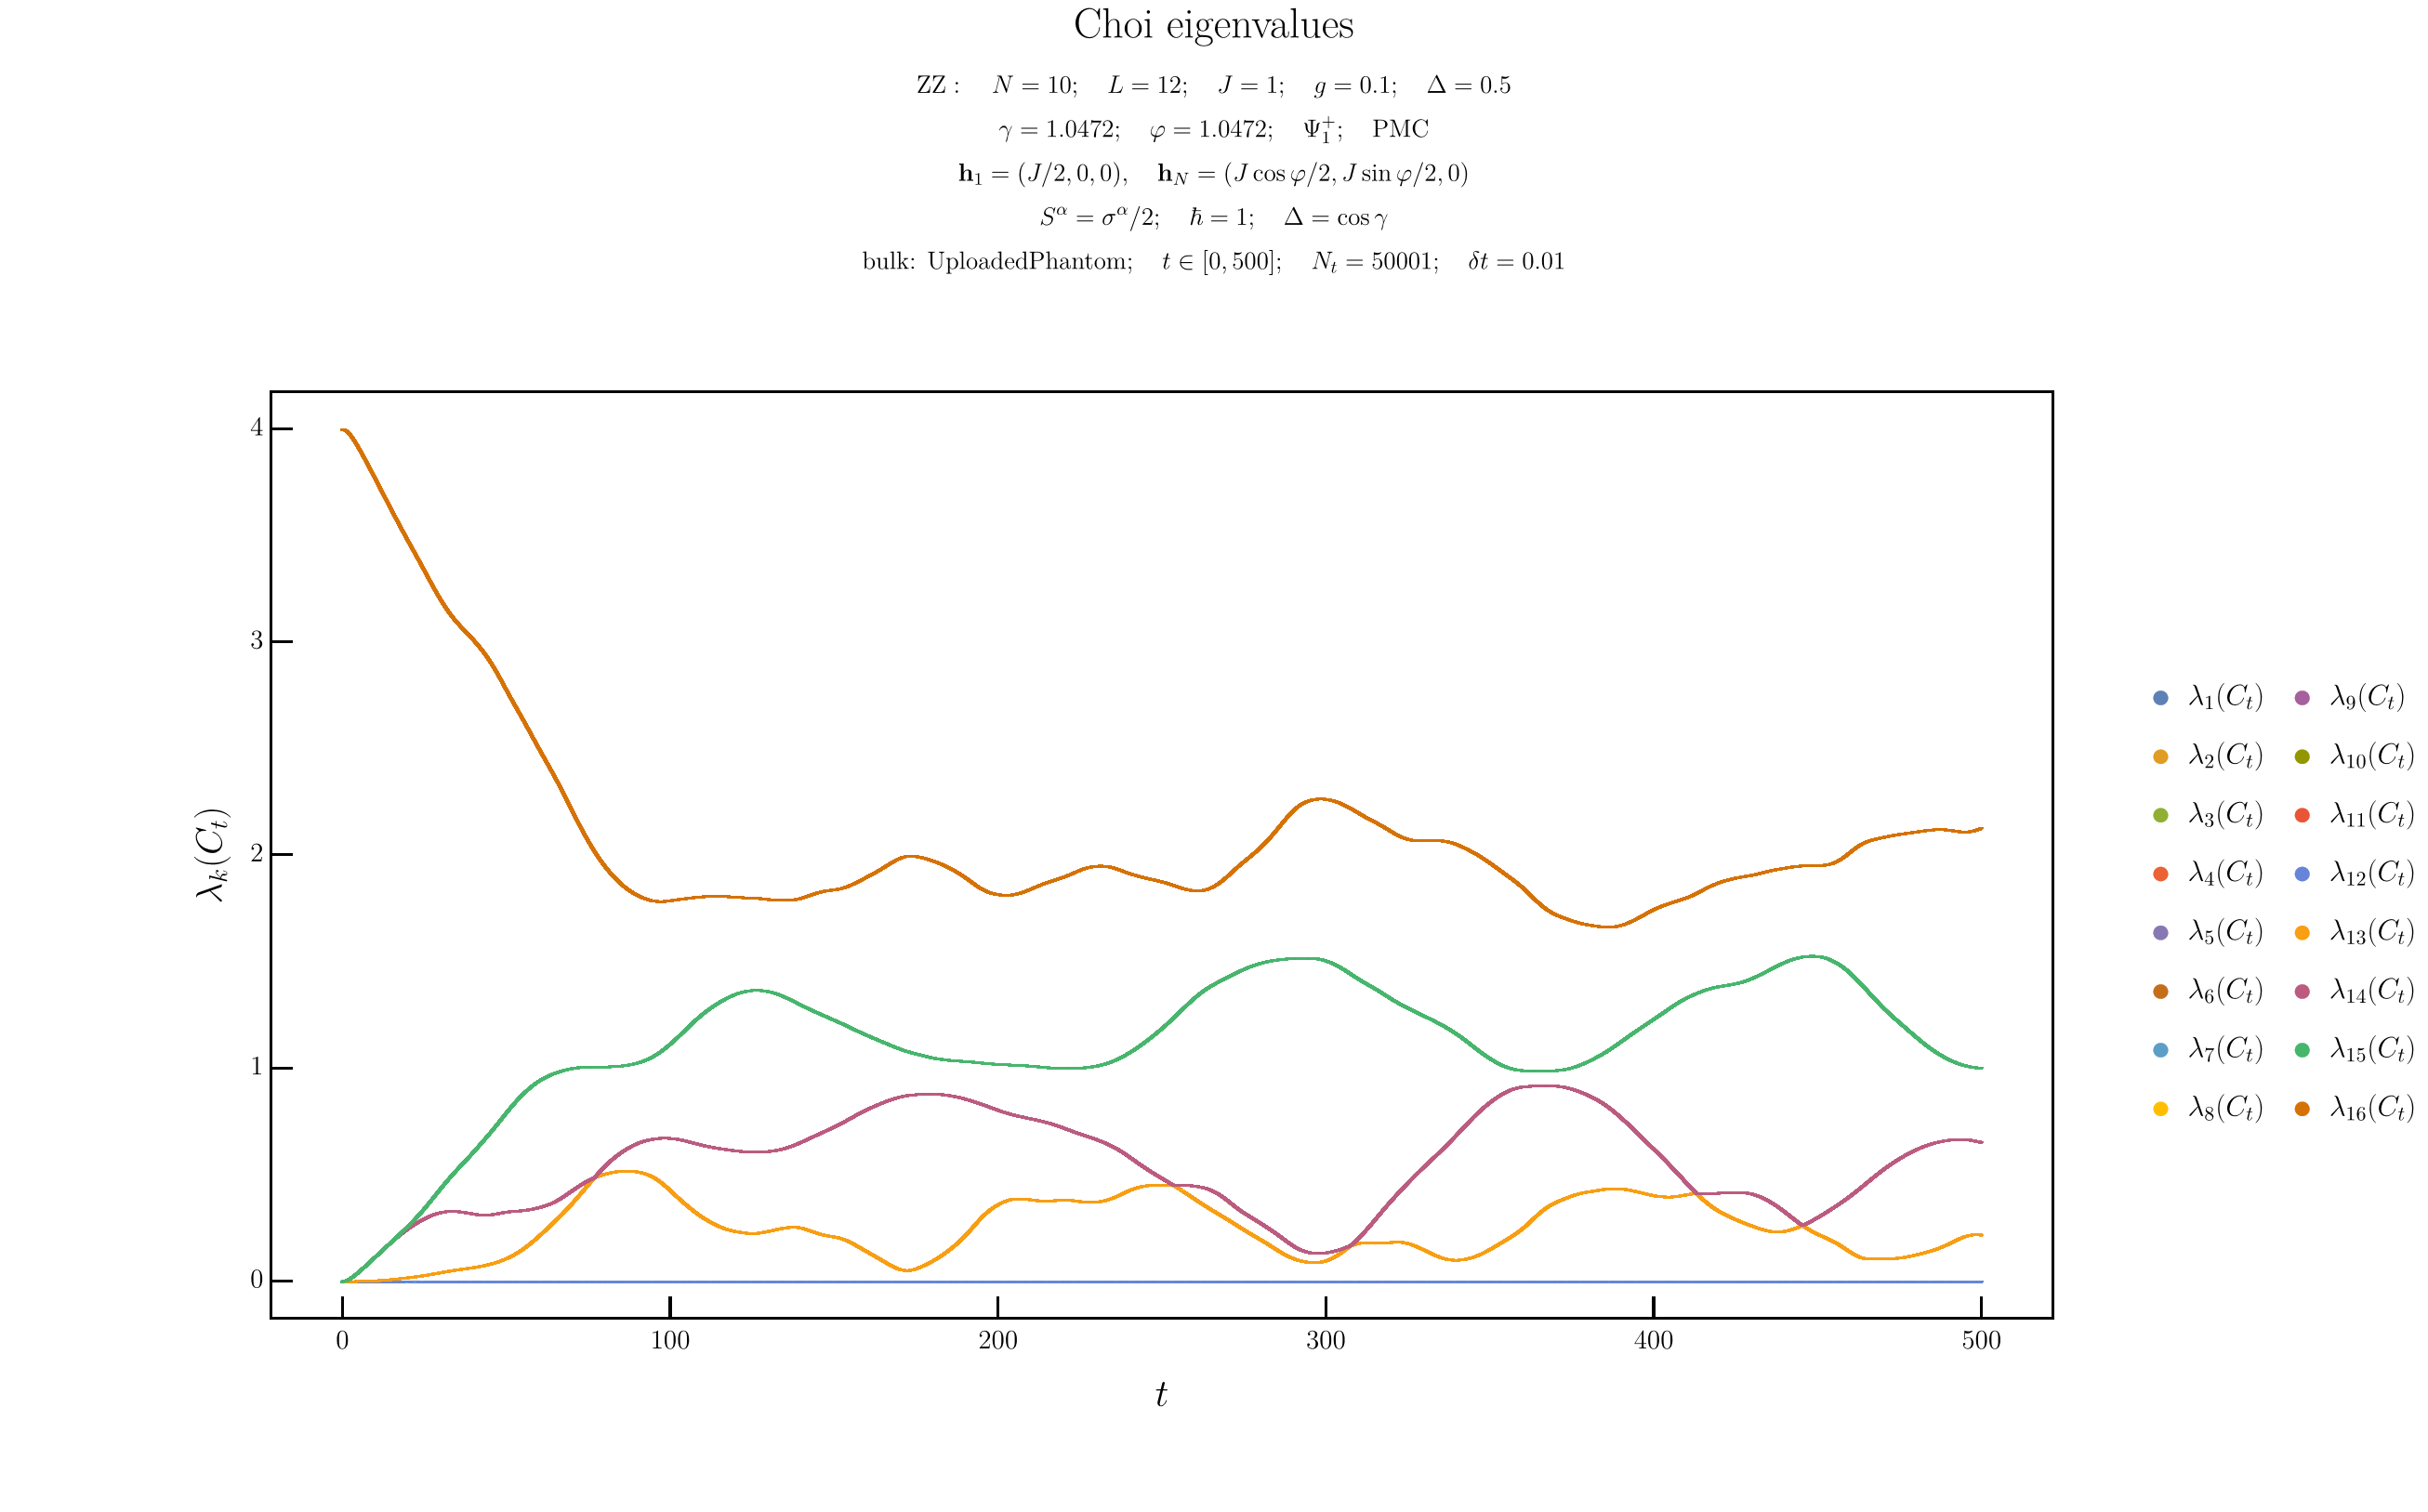
\includegraphics[width=\linewidth,height=0.77\textheight,keepaspectratio]{Phantom_ZZ_N10/Channel_ChoiEigenvalues.png}
\end{column}
\begin{column}{0.41\textwidth}
\footnotesize
\[
\spec C_t=\{0^{12}\}\cup\spec\Gamma,\quad \spec\Gamma=4\spec\rho_{AB}
\]
\begin{itemize}\setlength\itemsep{4pt}
\item \textbf{Four nonzero branches:} confirm Kraus rank $4$ ($t\ge 0.13$) and map entropy $S(C_t/4)\equiv S(\rho_{AB})$.
\item \textbf{Symmetry-protected crossings:} $\ket{\Phi^-}$ ($\mathcal R\mathcal F=-1$) carries exact eigenvalue $1-\Gamma_{00,11}(t)$ and crosses the smallest $\mathcal R\mathcal F=+1$ eigenvalue without level repulsion.
\item \textbf{Origin of kinks:} ascending sorting at every $t$ turns those exact crossings ($t=77.0, 253.4, 307.5, 413.1, 445.4$) into sharp kinks of $\lambda_{13},\lambda_{14}$ and $\lambda_{\min}$---sorting artefacts, not singular physics.
\end{itemize}
\end{column}
\end{columns}
\end{frame}

% ==============================================================
\begin{frame}{Reference--output Choi negativity}
\begin{columns}[T,totalwidth=\textwidth]
\begin{column}{0.57\textwidth}
\centering
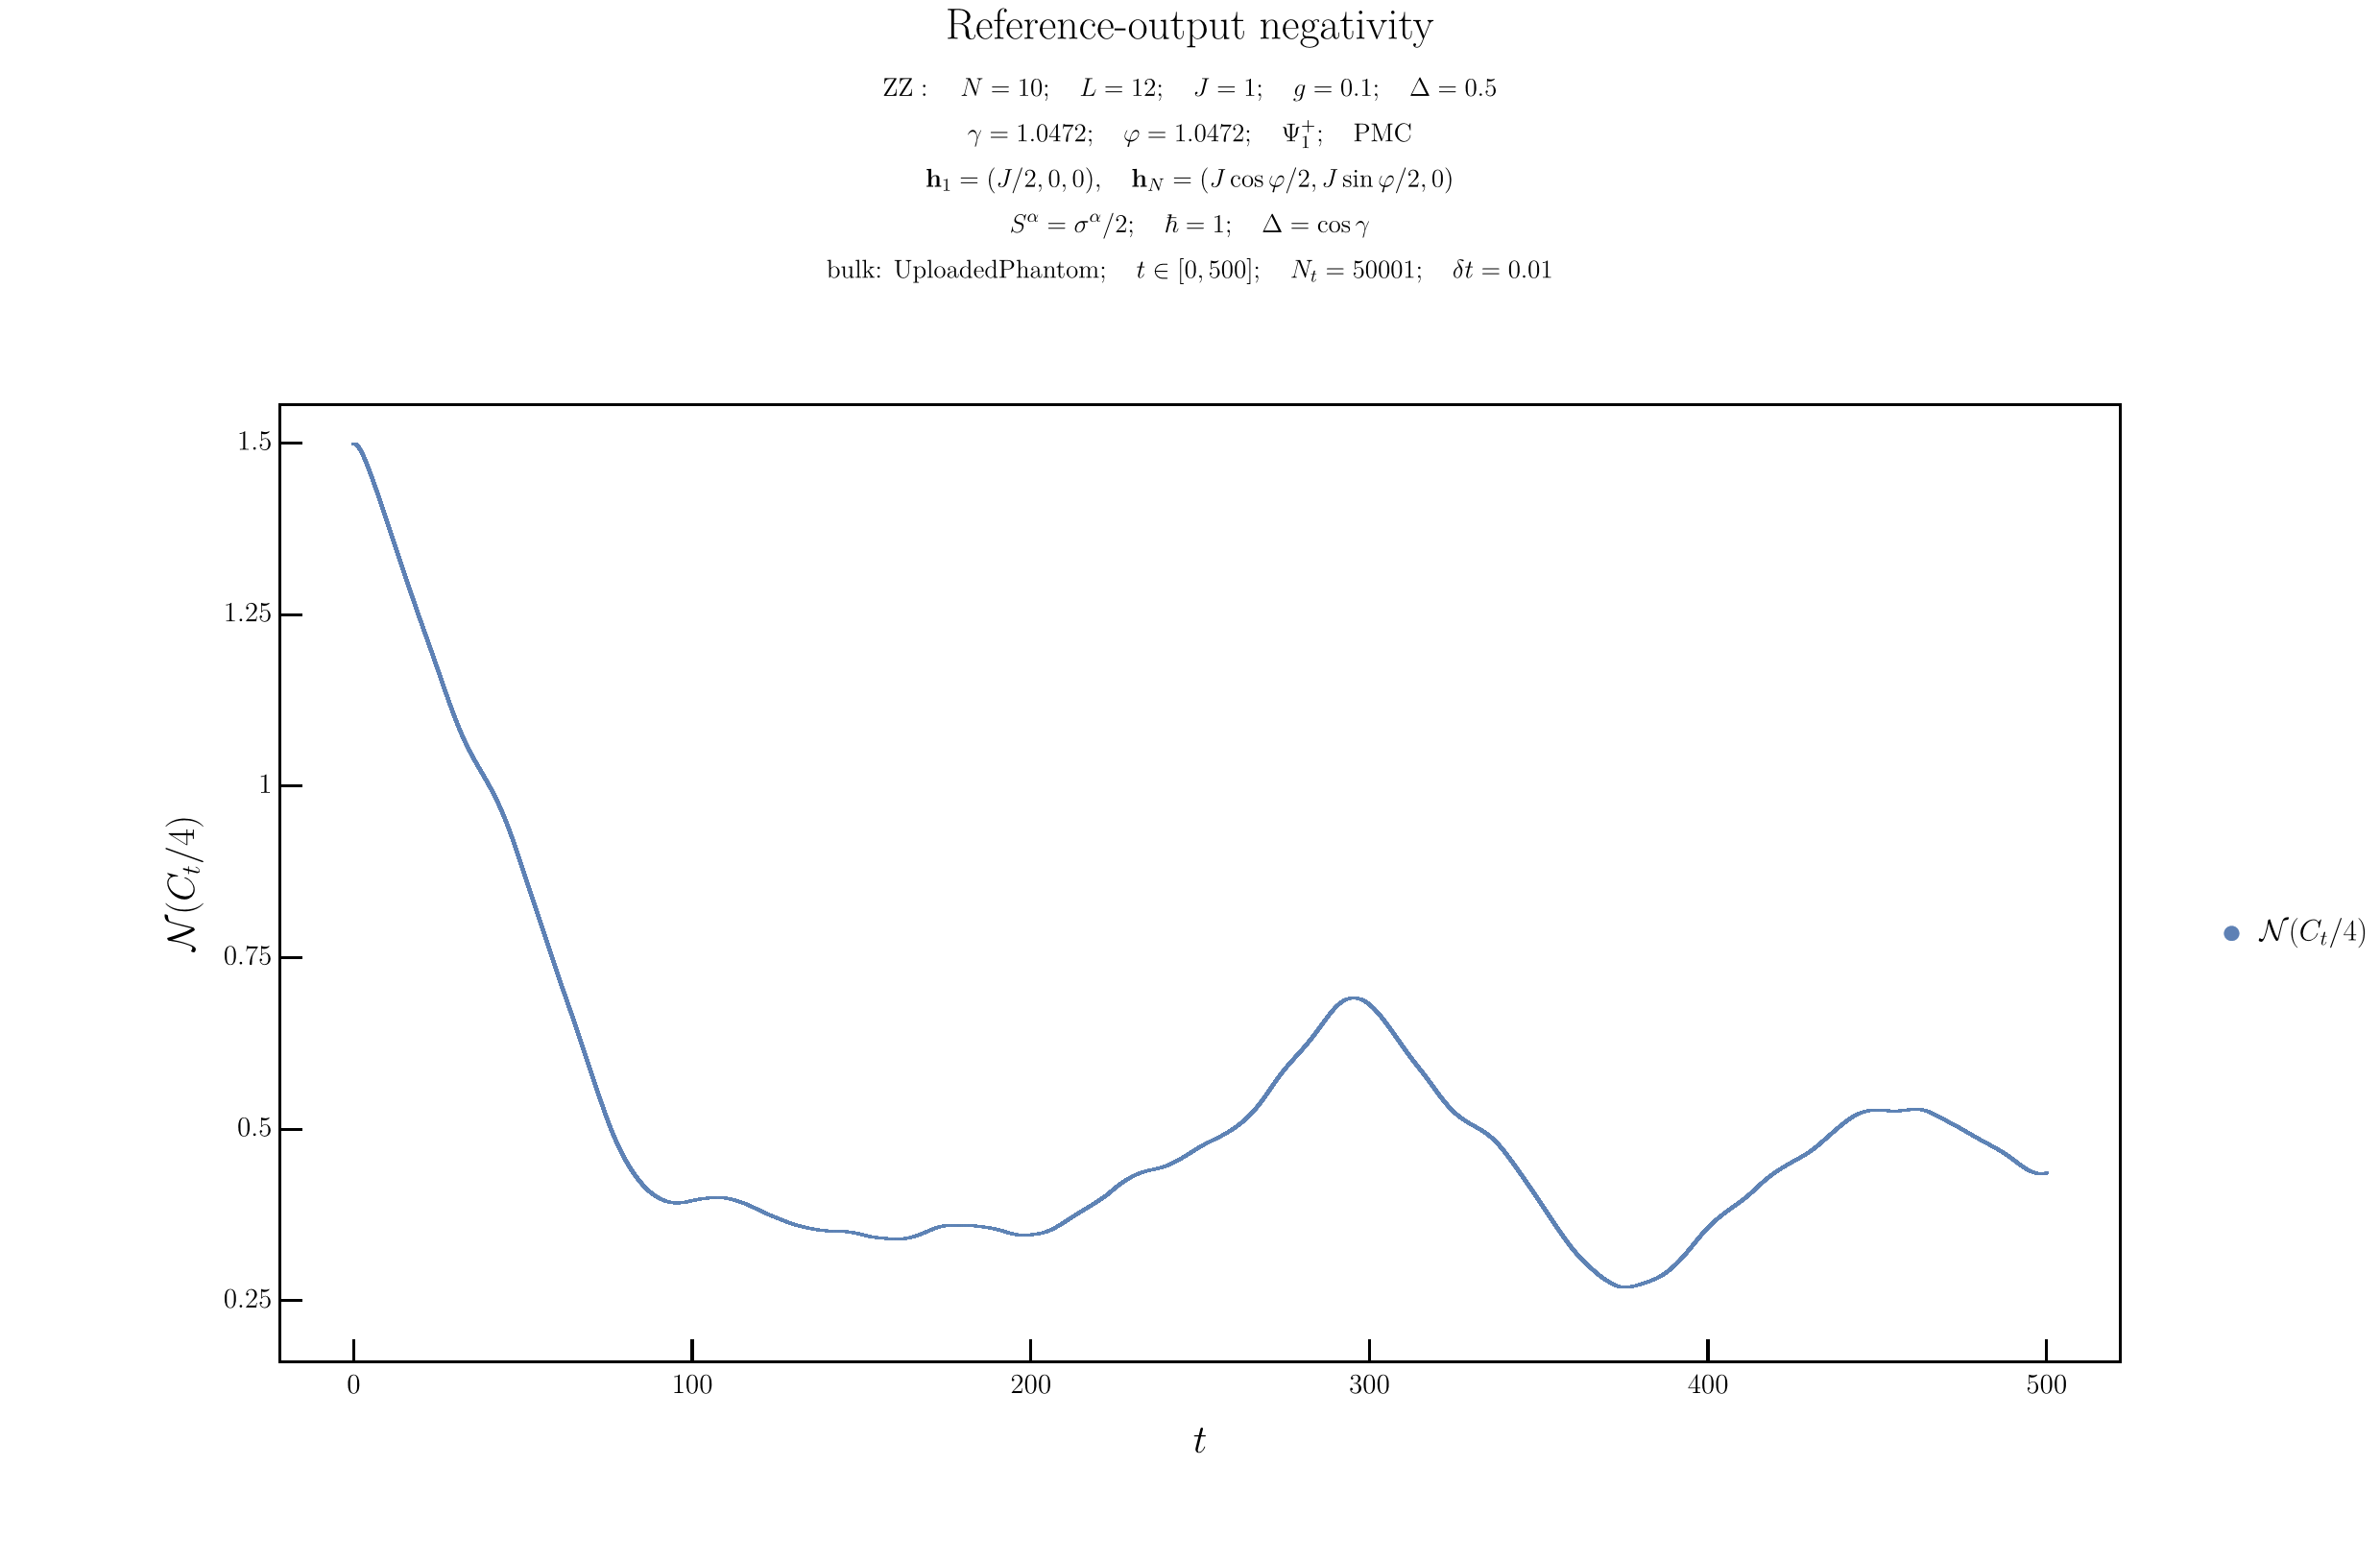
\includegraphics[width=\linewidth,height=0.77\textheight,keepaspectratio]{Phantom_ZZ_N10/Channel_ChoiNegativity.png}
\end{column}
\begin{column}{0.41\textwidth}
\footnotesize
\[
\mathcal N(\omega_t)=\tfrac12\bigl(\lVert\omega_t^{T_{\mathrm{out}}}\rVert_1-1\bigr)=\tfrac14\textstyle\sum_{a<b}\lvert\Gamma_{ab}\rvert .
\]
\begin{itemize}\setlength\itemsep{5pt}
\item \textbf{Exact $\ell_1$-coherence:} starts at $6/4=1.5$ ($t=0$, noiseless identity channel), dips to $0.271$ at $t=375.4$, and revives to $0.692$ at $t=295.4$.
\item \textbf{Bipartition caveat:} measures entanglement between \textbf{reference $R$ and output $AB$}---how well $\Lambda_t$ preserves input coherence---\emph{not} entanglement between physical edges $A$ and $B$.
\item \textbf{Smoothness:} completely smooth across $t=222.60$.
\end{itemize}
\end{column}
\end{columns}
\end{frame}

% ==============================================================
\begin{frame}{Invertibility of $\Lambda_t$ and log-scale conditioning}
\begin{columns}[T,totalwidth=\textwidth]
\begin{column}{0.57\textwidth}
\centering
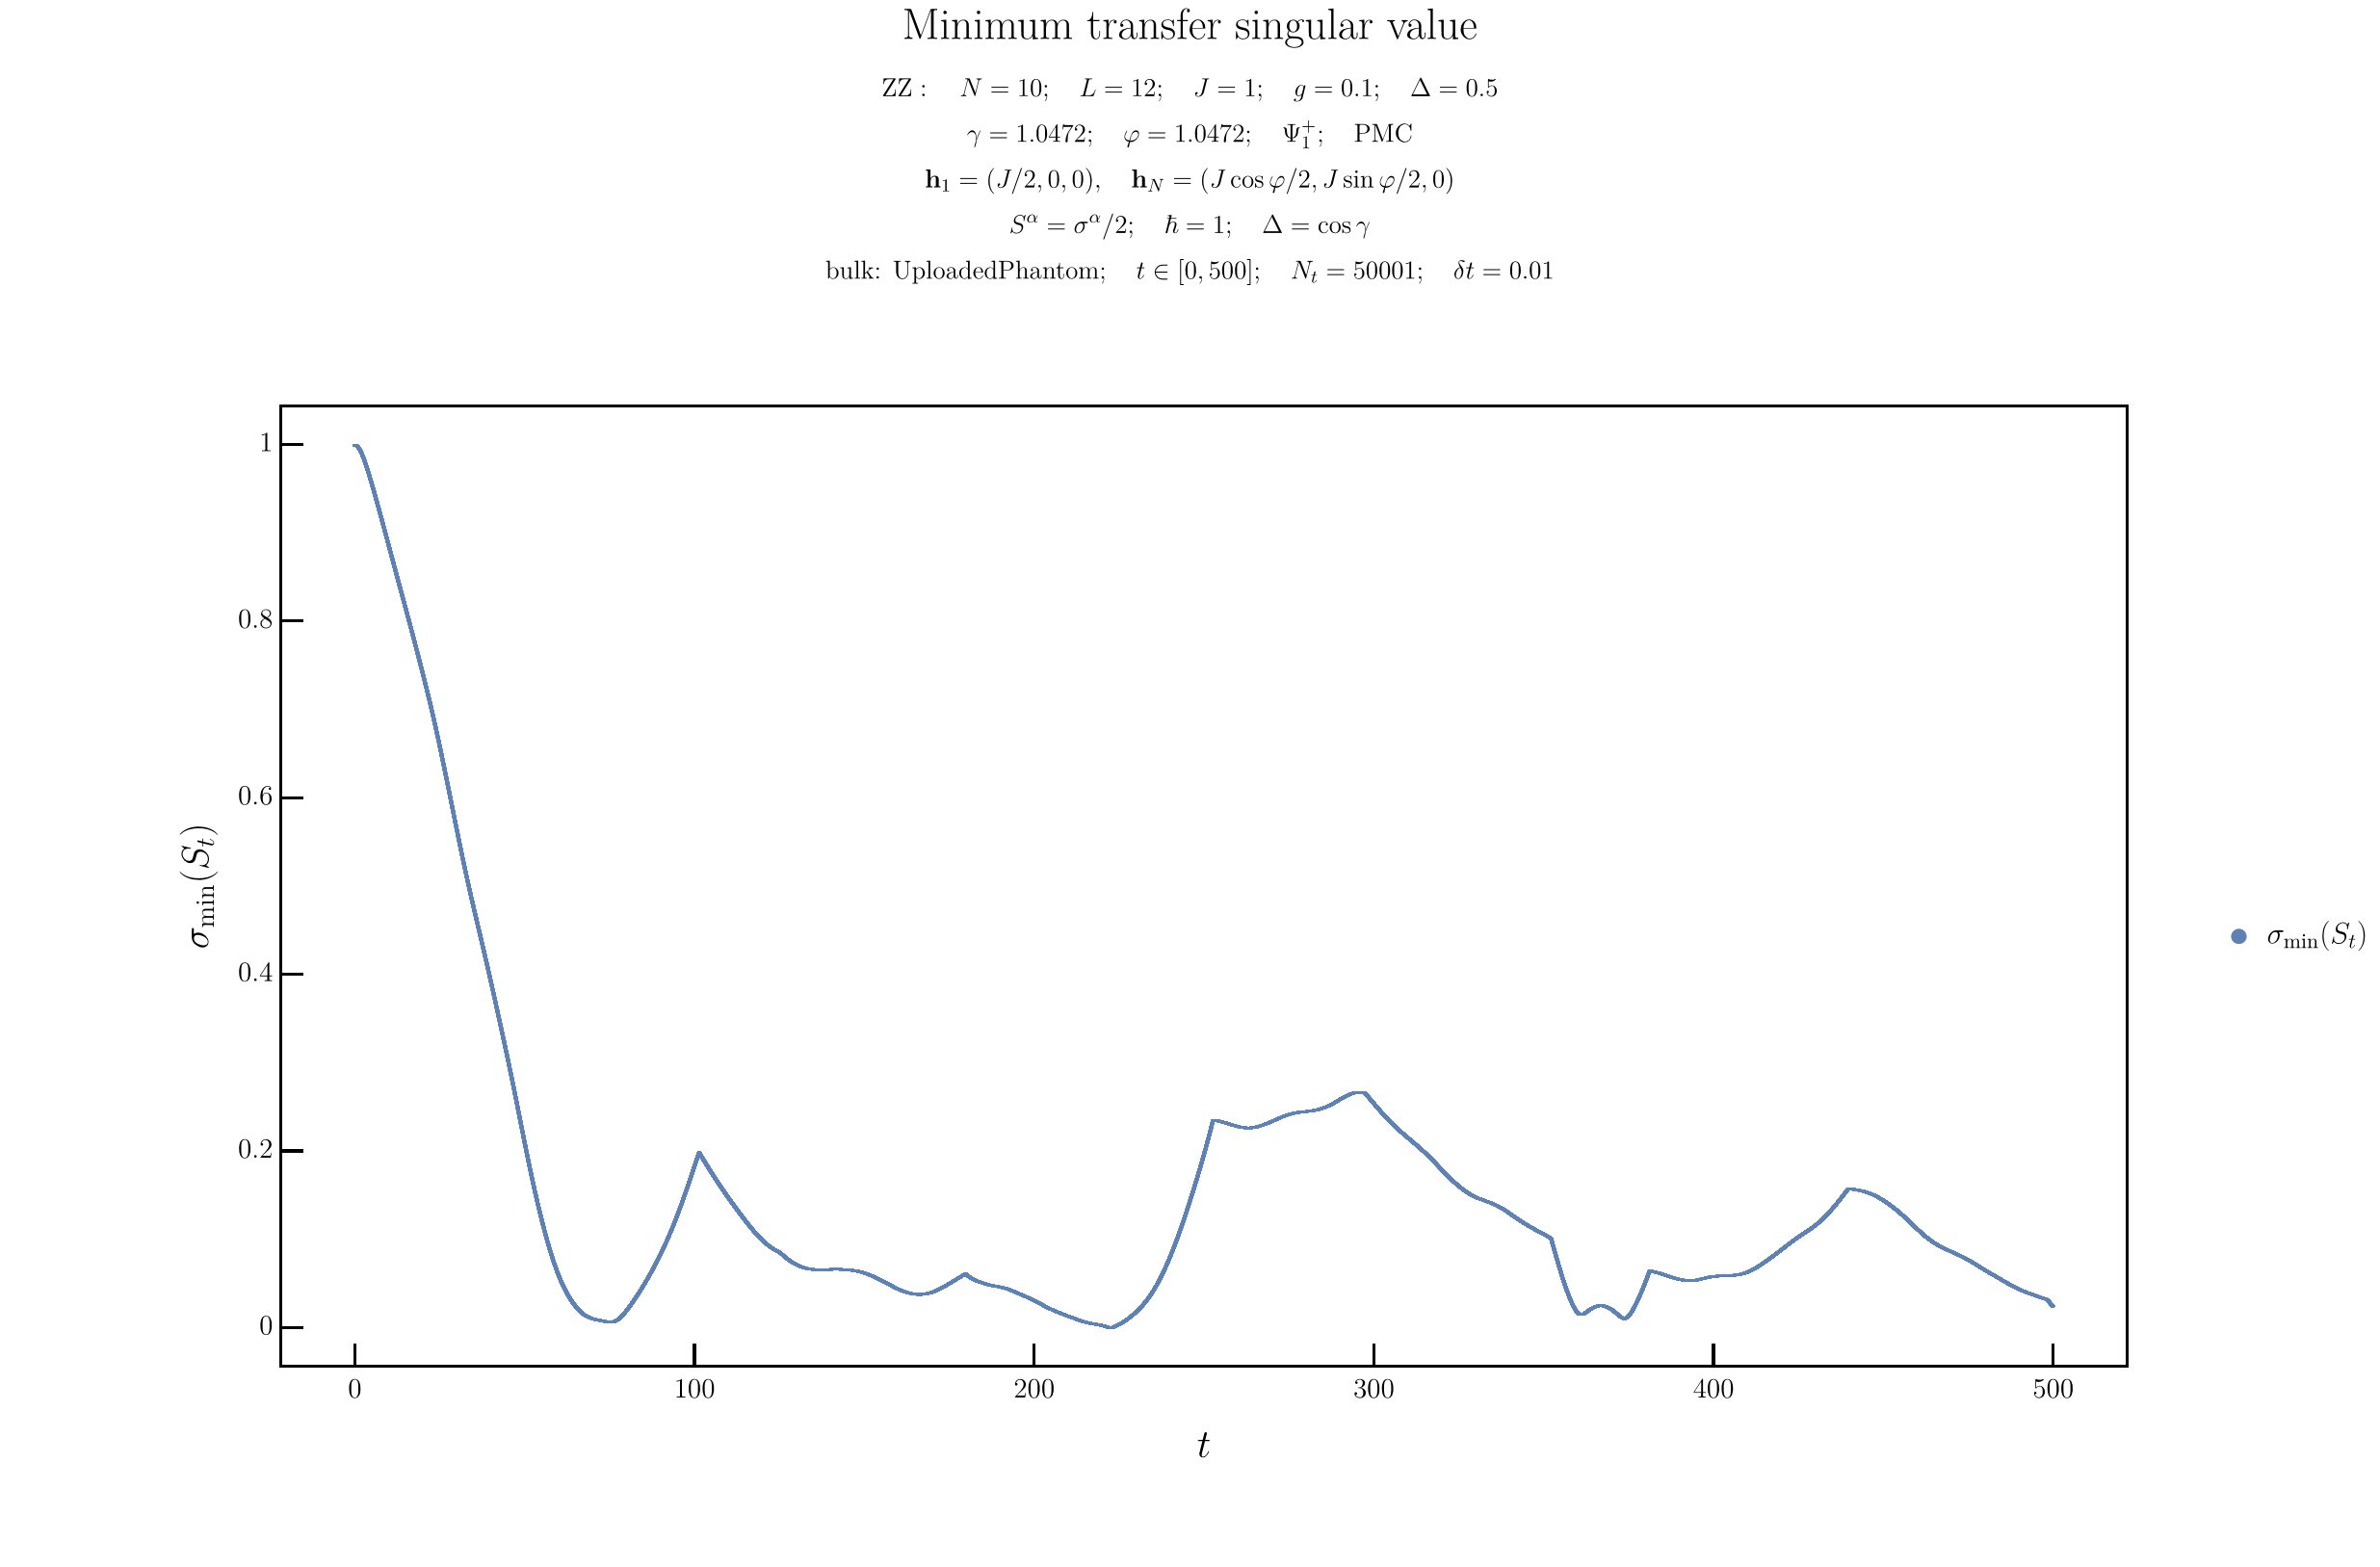
\includegraphics[width=\linewidth,height=0.40\textheight,keepaspectratio]{Phantom_ZZ_N10/Channel_MinSingularValue.png}\\[2pt]
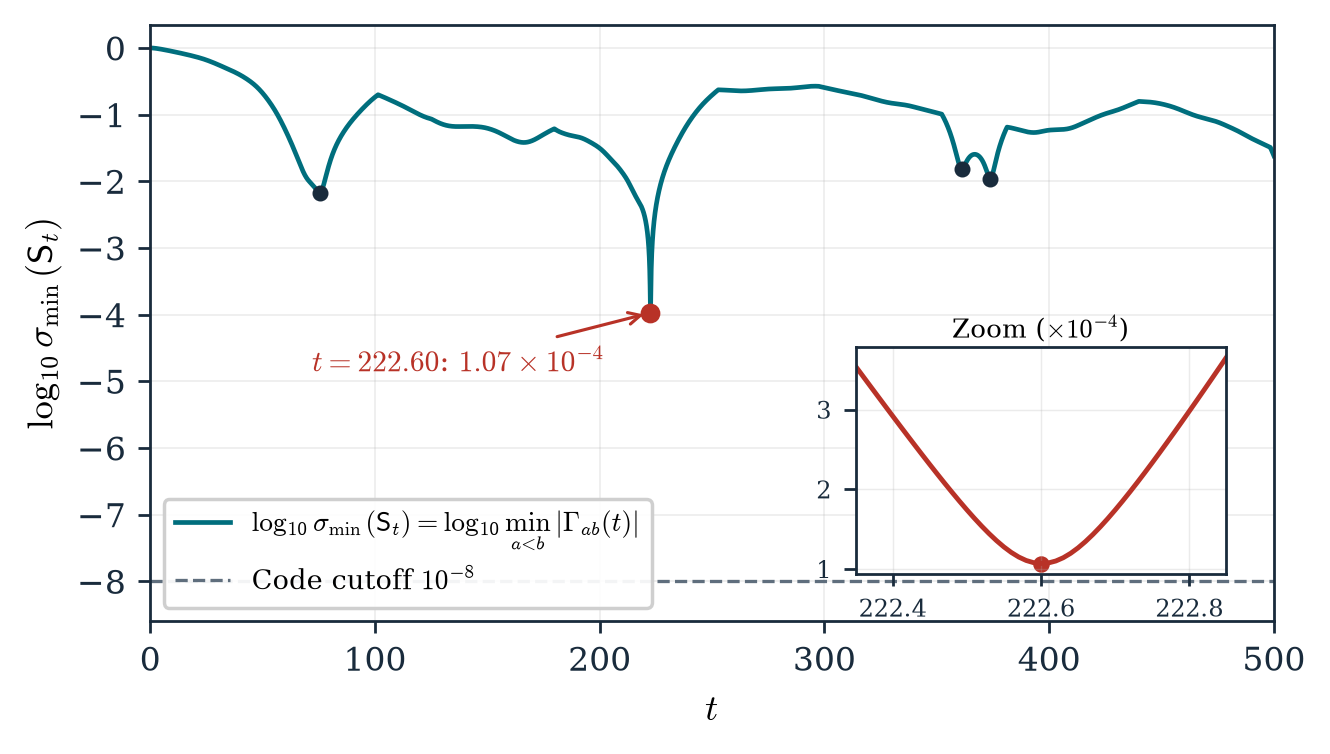
\includegraphics[width=\linewidth,height=0.40\textheight,keepaspectratio]{Phantom_ZZ_N10/new/minsv_log.png}
\end{column}
\begin{column}{0.41\textwidth}
\footnotesize
\[
\sigma_{\min}(\St)=\min_{a<b}\lvert\Gamma_{ab}(t)\rvert .
\]
\begin{itemize}\setlength\itemsep{4pt}
\item \textbf{Four near-zeros:} governed by $\lvert\Gamma_{01,10}(t)\rvert$ at $t=75.37$, $222.60$, $361.09$, and $373.80$ (slope kinks mark switches of the minimizing pair $a<b$).
\item \textbf{Deepest dip resolved:} $\min_t\sigma_{\min}(\St)=1.07\times 10^{-4}$ at $t=222.60$ ($\operatorname{Re}=-1.6\times 10^{-5}$, $\operatorname{Im}=-1.05\times 10^{-4}\neq 0$).
\item \textbf{Invertible throughout:} stays $4$ orders of magnitude above the $10^{-8}$ cutoff, so $\Lambda_t^{-1}$ is well-defined at every sample.
\end{itemize}
\end{column}
\end{columns}
\end{frame}

% ==============================================================
\begin{frame}{Canonical master-equation rates}
\begin{columns}[T,totalwidth=\textwidth]
\begin{column}{0.57\textwidth}
\centering
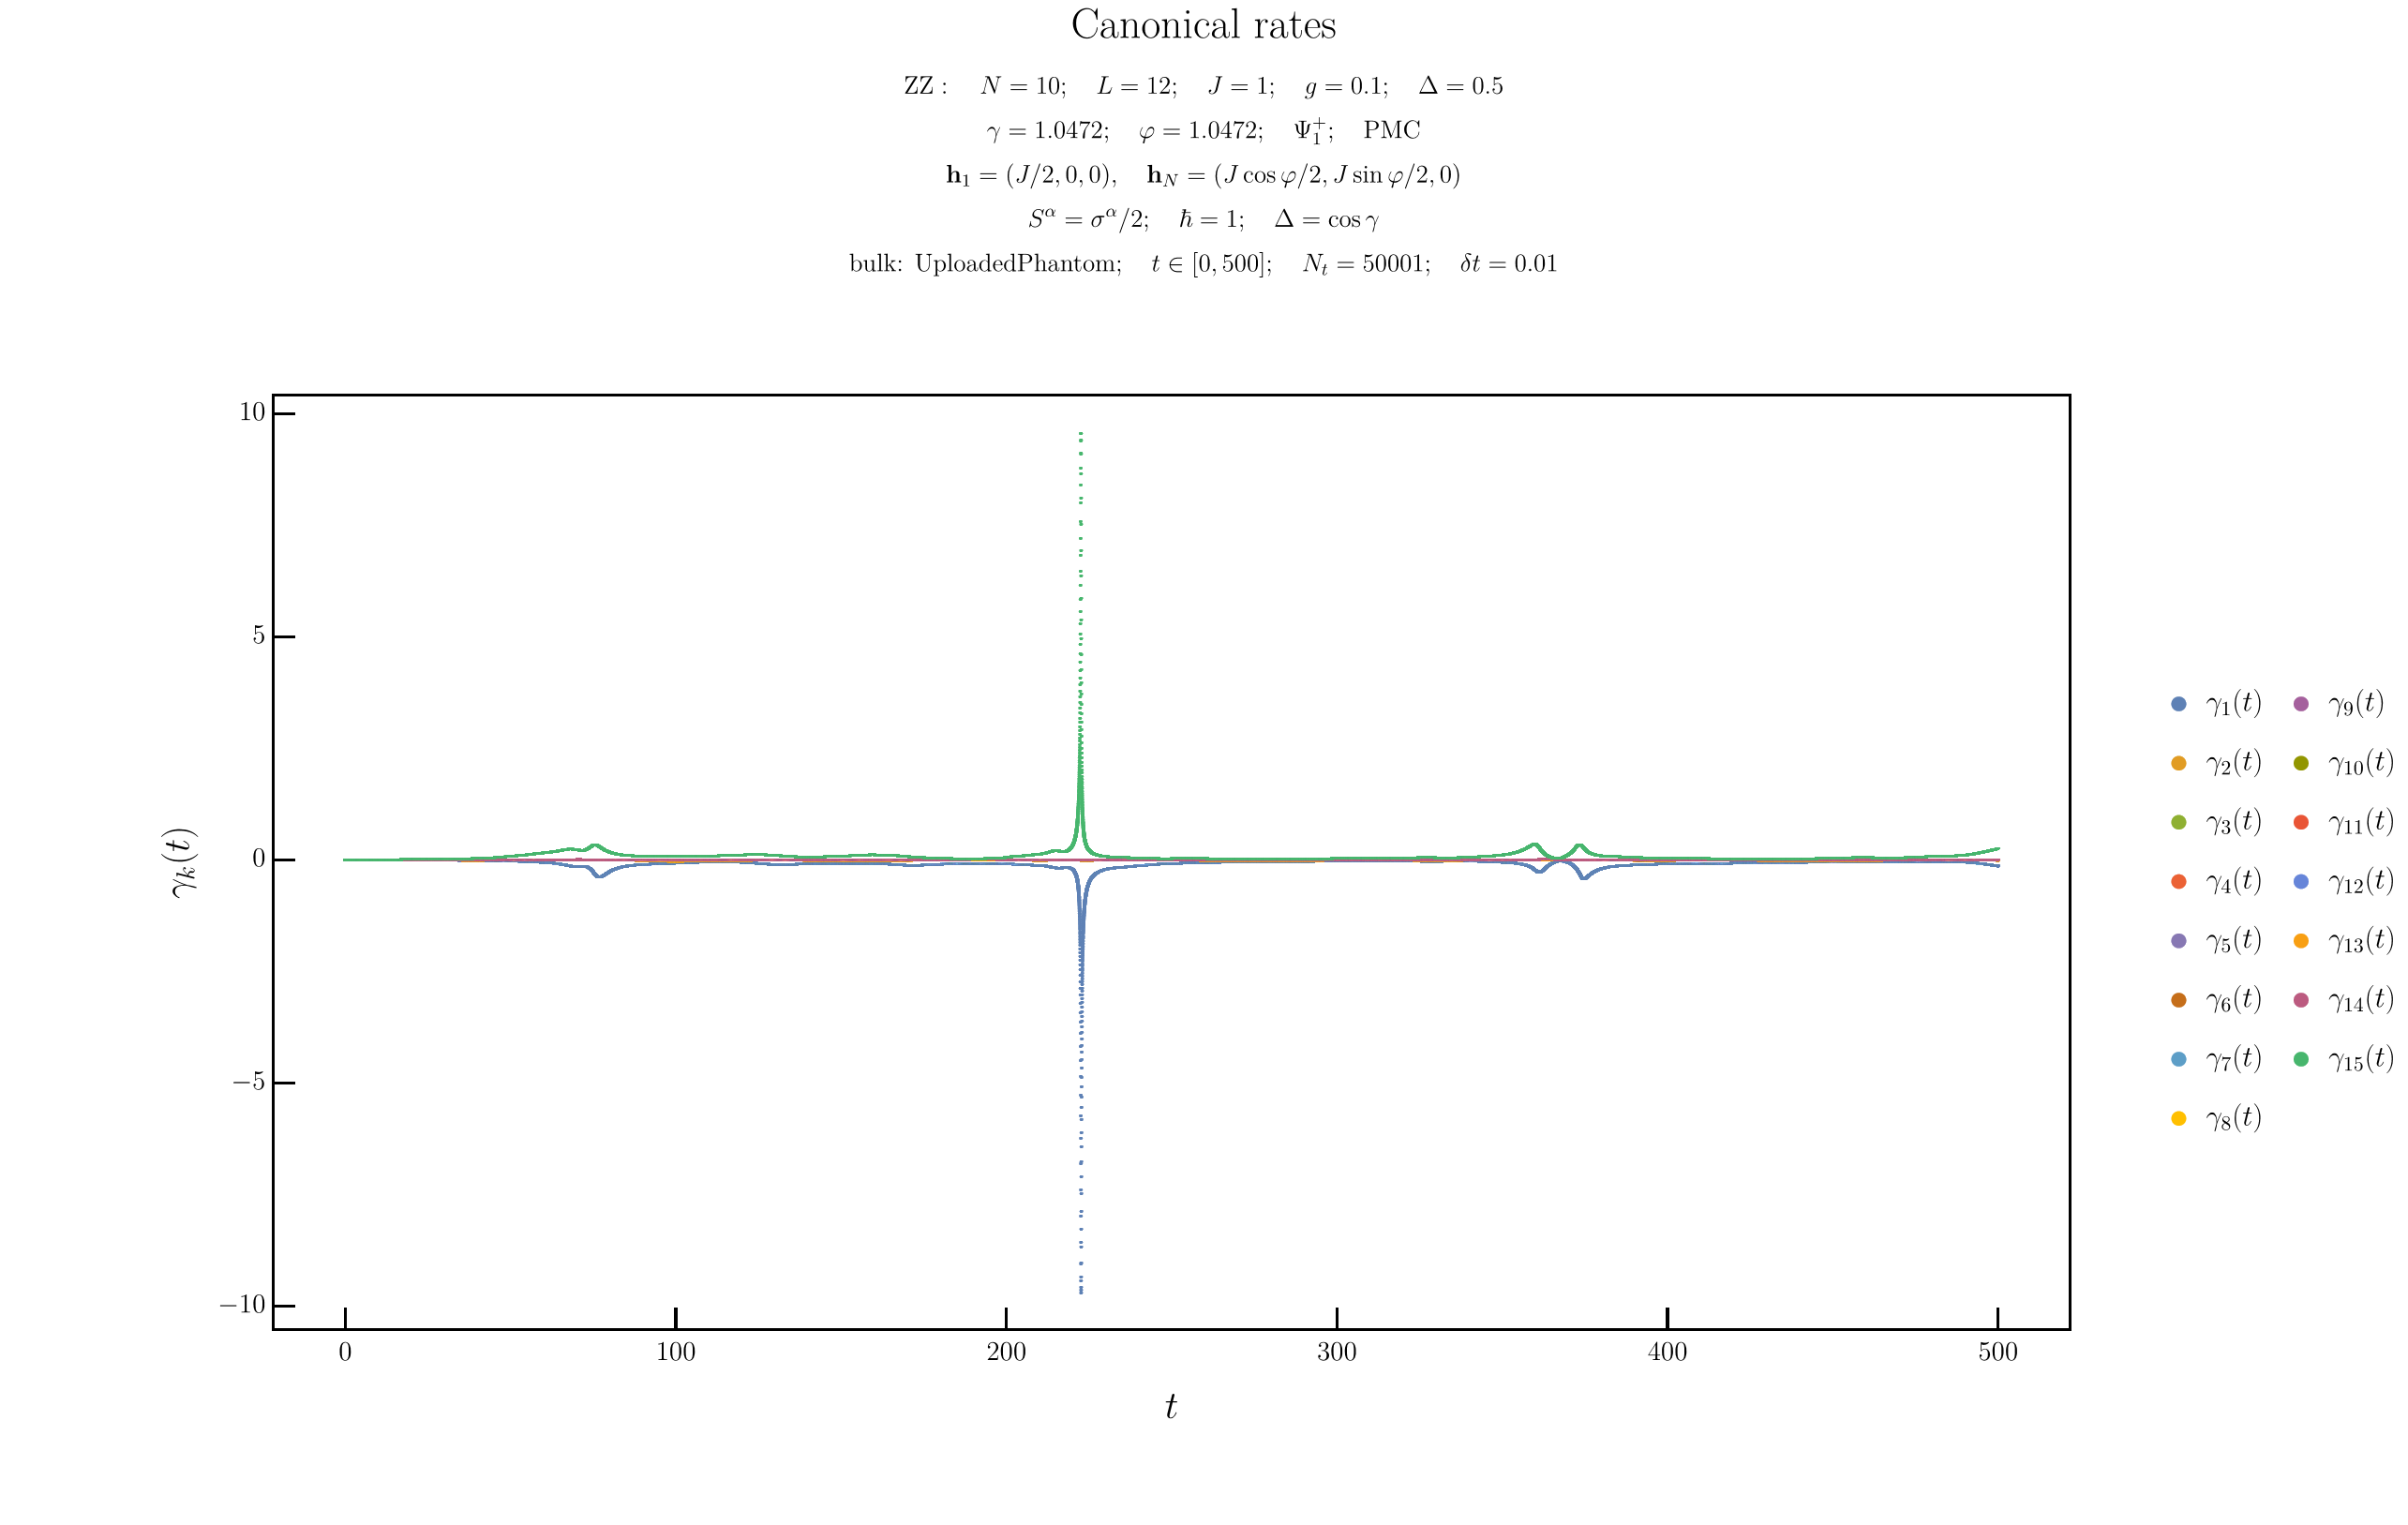
\includegraphics[width=\linewidth,height=0.77\textheight,keepaspectratio]{Phantom_ZZ_N10/Channel_CanonicalRates.png}
\end{column}
\begin{column}{0.41\textwidth}
\footnotesize
\[
\{\gamma_k\}_{k=1}^{15}=\operatorname{sort}\!\bigl(\spec(G^{\mathsf T}[\dot\Gamma\oslash\Gamma]G)\cup\{0^{\times 12}\}\bigr).
\]
\begin{itemize}\setlength\itemsep{4pt}
\item \textbf{Tall finite spike at $t\approx 222.6$:} $\gamma_{15}(t)$ peaks at \textbf{$+9.57$} ($t=222.58$, decay into the dip) and $\gamma_1(t)$ reaches \textbf{$-9.69$} ($t=222.63$, revival out of the dip) in a near-mirror pair.
\item \textbf{Minor bumps:} $\lvert\gamma_{1,15}\rvert\approx 0.27$--$0.42$ at $t\approx 76, 361, 374$, matching the shallower near-zeros of $\lvert\Gamma_{01,10}\rvert$.
\item \textbf{Remaining $13$ curves:} the third active eigenvalue stays tiny ($\lvert\gamma_{2,14}\rvert\le 0.025$), and $\gamma_3=\cdots=\gamma_{13}\equiv 0$.
\end{itemize}
\end{column}
\end{columns}
\end{frame}

% ==============================================================
\begin{frame}{RHP CP-divisibility witnesses}
\begin{columns}[T,totalwidth=\textwidth]
\begin{column}{0.57\textwidth}
\centering
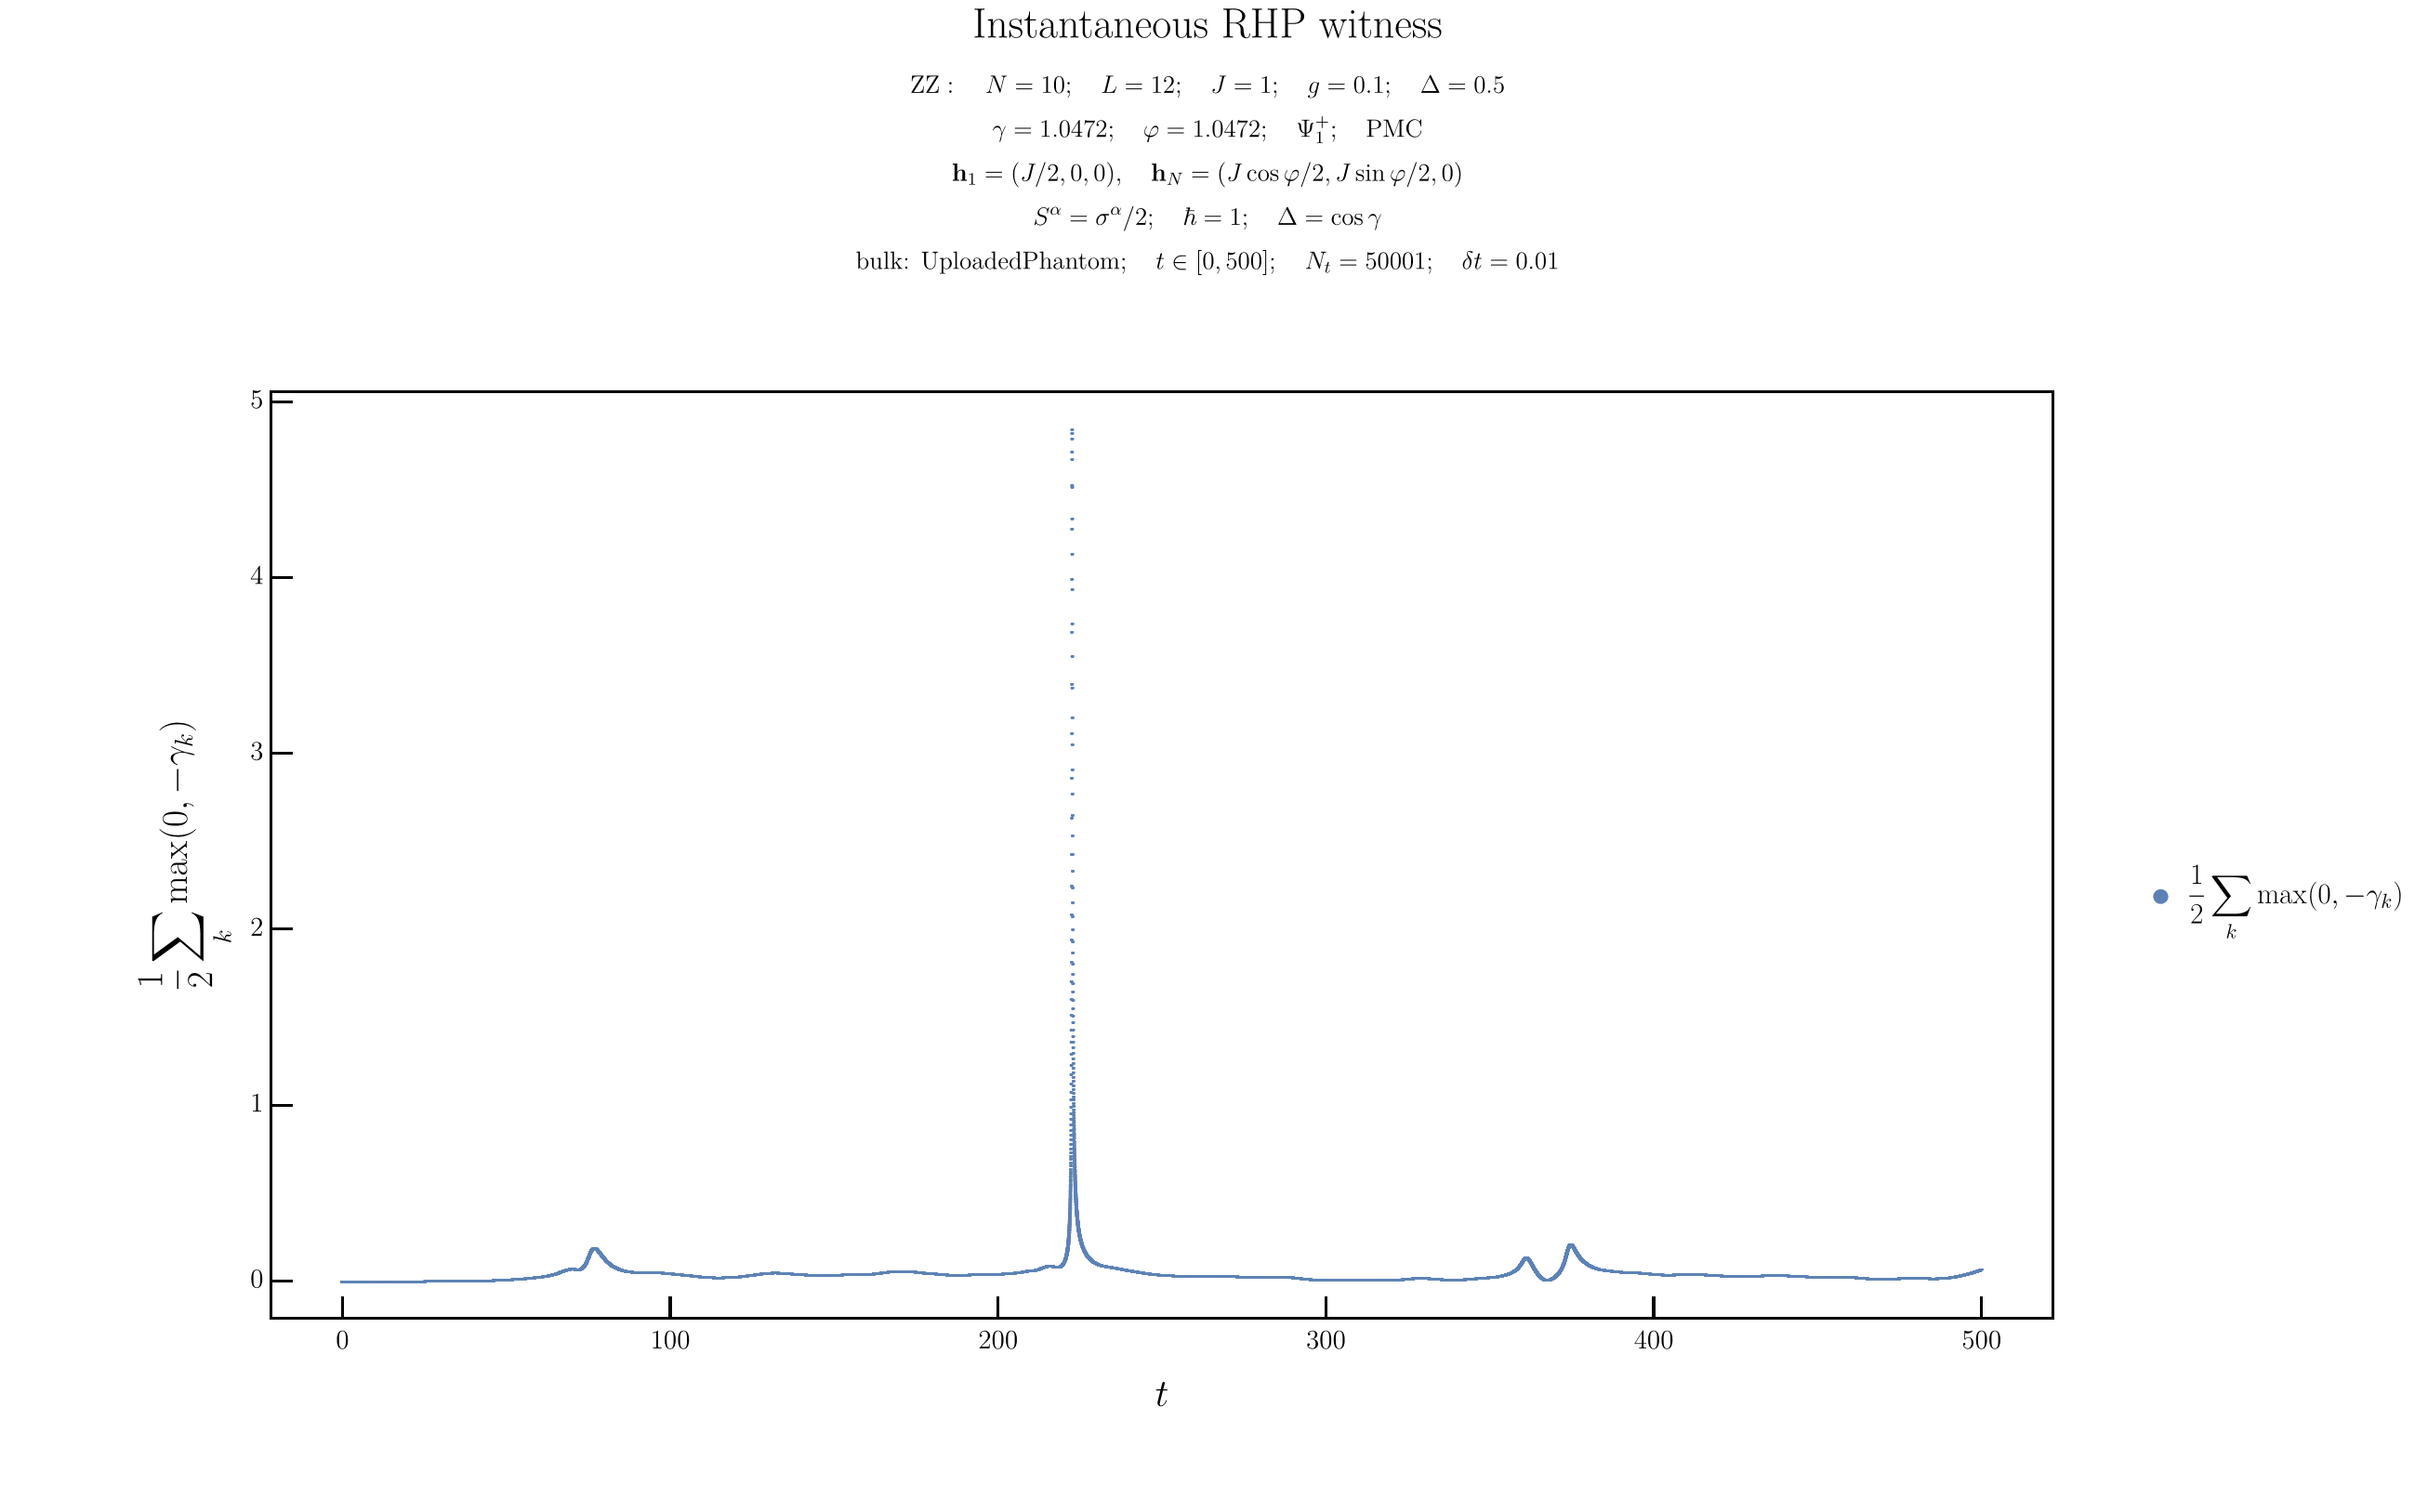
\includegraphics[width=\linewidth,height=0.41\textheight,keepaspectratio]{Phantom_ZZ_N10/Channel_RHPInstantaneous.png}\\[2pt]
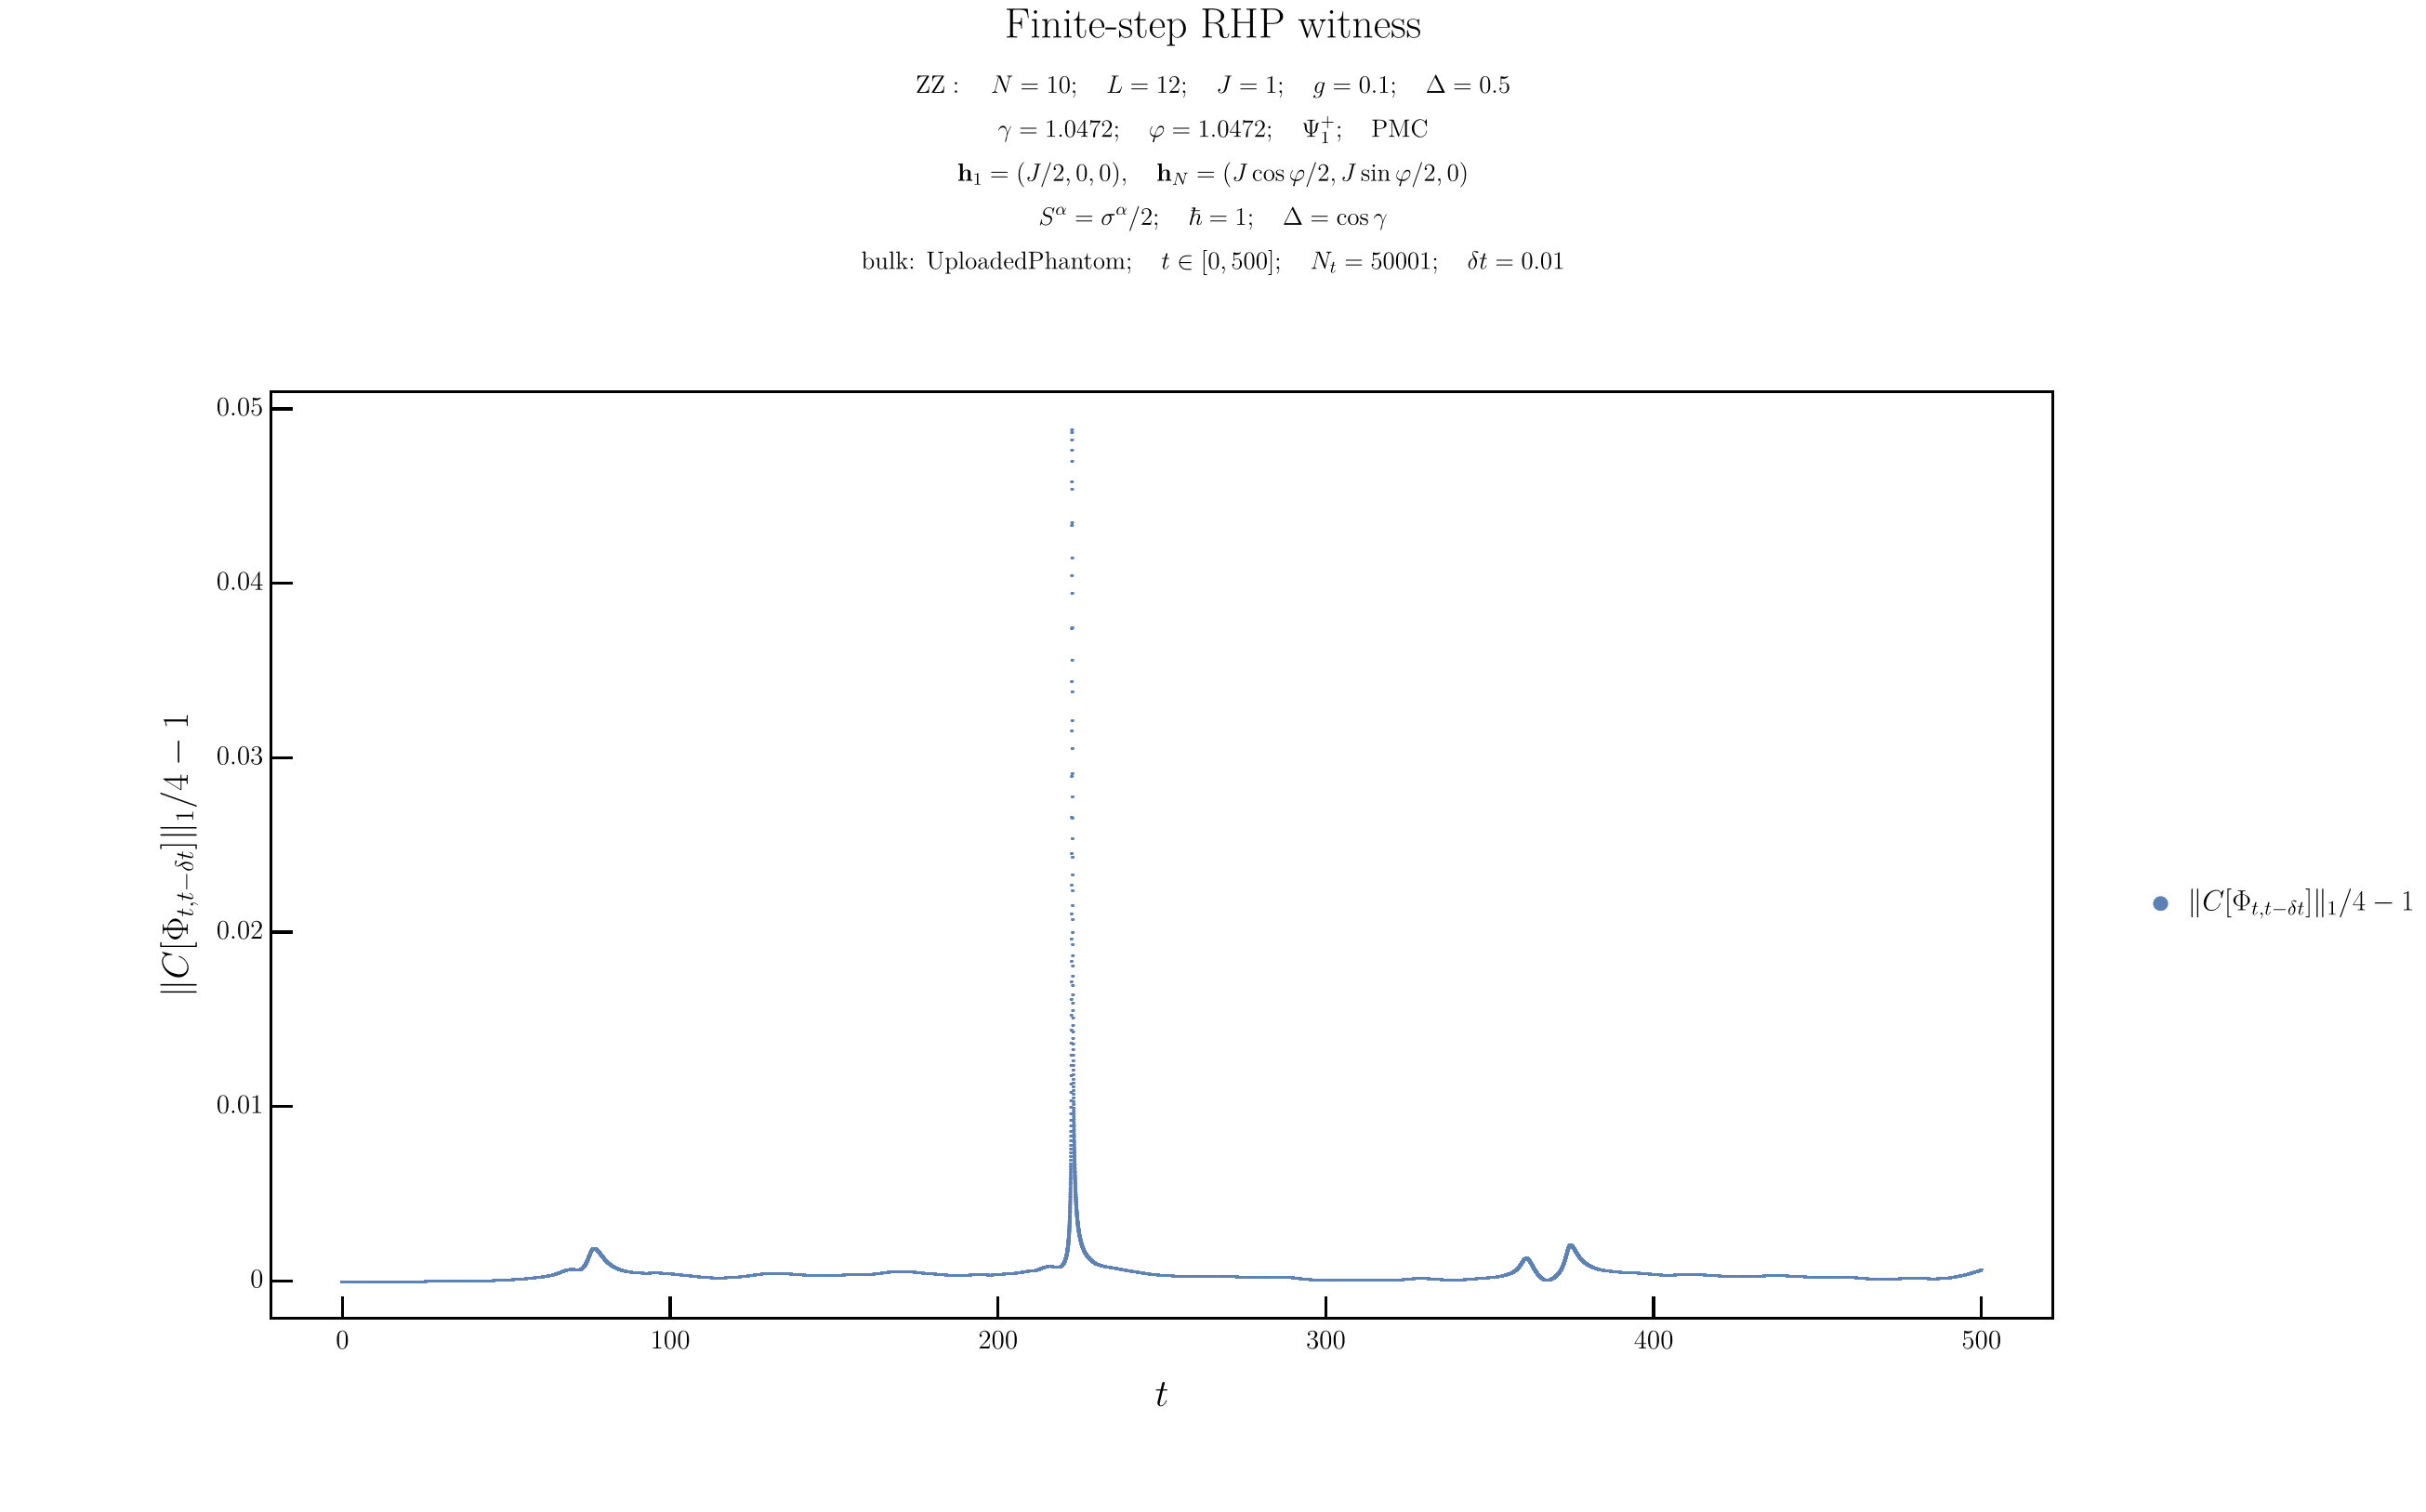
\includegraphics[width=\linewidth,height=0.39\textheight,keepaspectratio]{Phantom_ZZ_N10/Channel_RHPFiniteStep.png}
\end{column}
\begin{column}{0.41\textwidth}
\footnotesize
\[
g_{\mathrm{RHP}}(t)=\tfrac12\sum_k\max(0,-\gamma_k(t))\approx \frac{w_k}{\delta t}.
\]
\begin{itemize}\setlength\itemsep{4pt}
\item \textbf{Sharp spike at $t=222.63$:} $g_{\mathrm{RHP}}\approx -\gamma_1/2$ reaches \textbf{$4.84$}, while finite-step $w_k$ reaches \textbf{$0.0489$} at $t=222.64$ (rate $r_k=w_k/\delta t=4.89$, Appendix~2c).
\item \textbf{Secondary peaks:} $g_{\mathrm{RHP}}=0.19$, $0.13$, and $0.21$ at $t=76.9, 361.2, 374.7$.
\item \textbf{Interpretation:} CP-divisibility is strongly violated as $\lvert\Gamma_{01,10}\rvert$ rebounds from its near-zero, while $\Lambda_t$ remains CPTP at all times.
\end{itemize}
\end{column}
\end{columns}
\end{frame}

% ==============================================================
\begin{frame}{BLP state-distinguishability witness}
\footnotesize
\begin{columns}[T,totalwidth=\textwidth]
\begin{column}{0.49\textwidth}
\centering
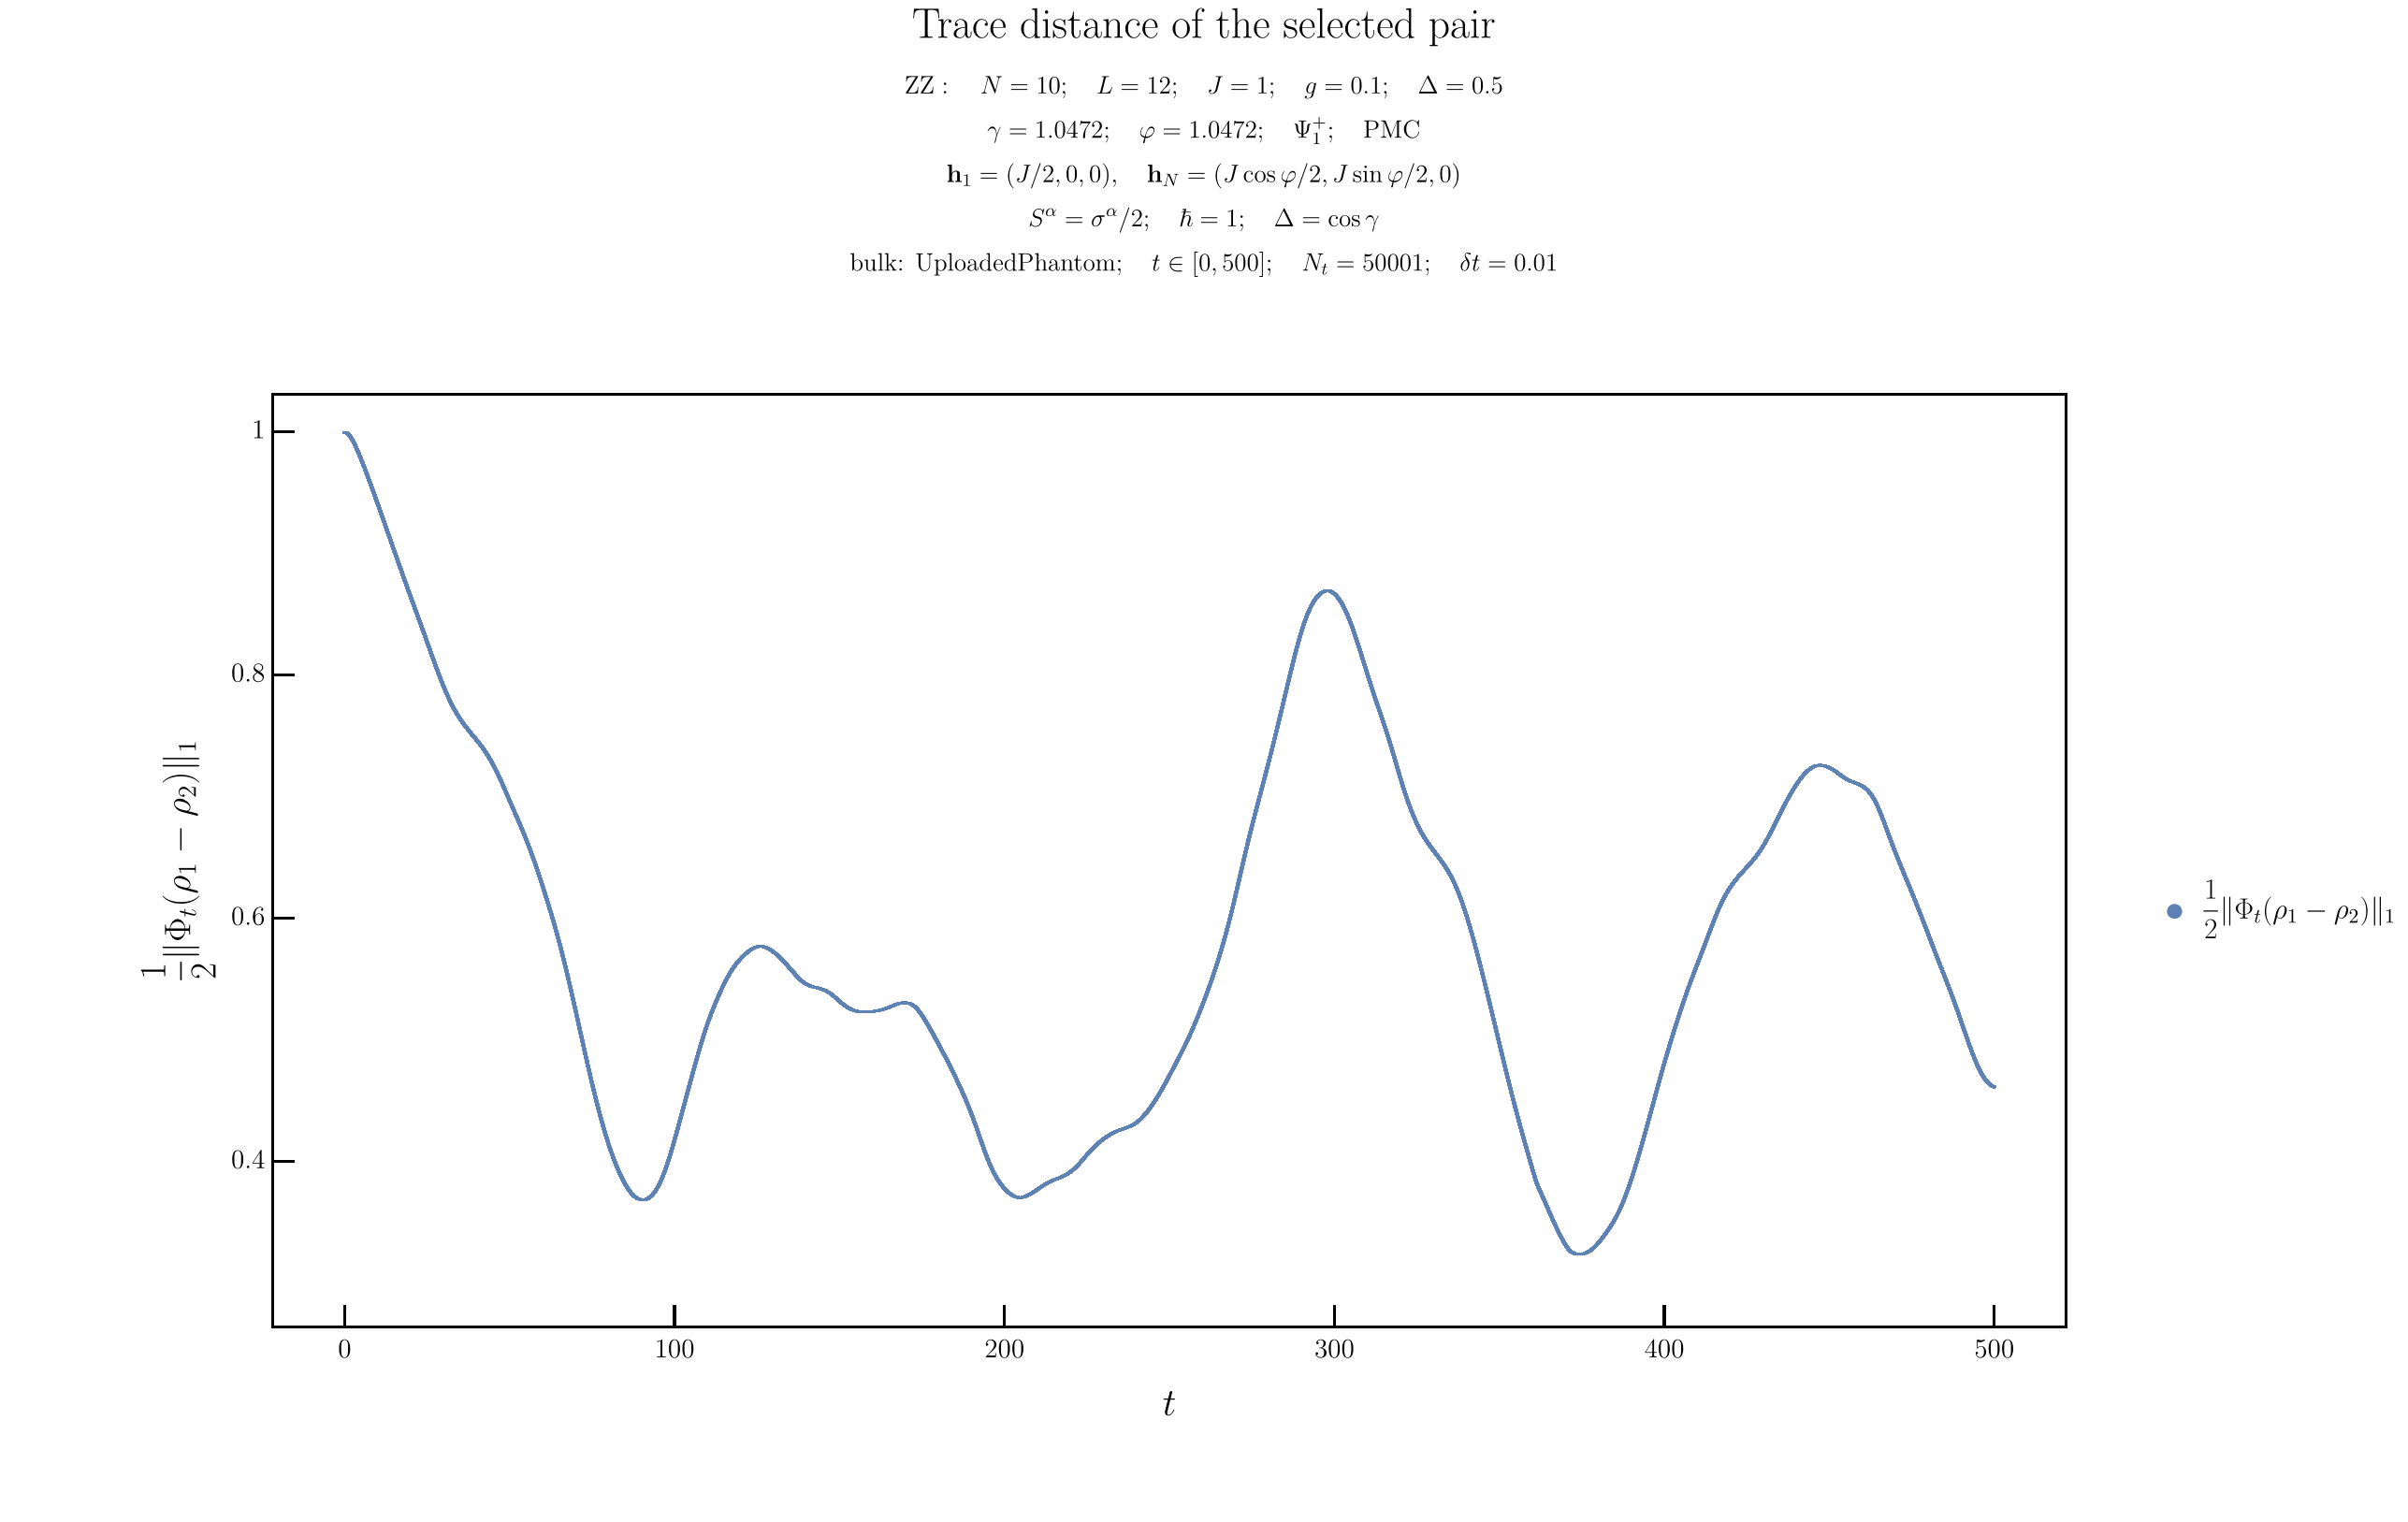
\includegraphics[width=\linewidth,height=0.49\textheight,keepaspectratio]{Phantom_ZZ_N10/Channel_BLPDistance.png}
\end{column}
\begin{column}{0.49\textwidth}
\centering
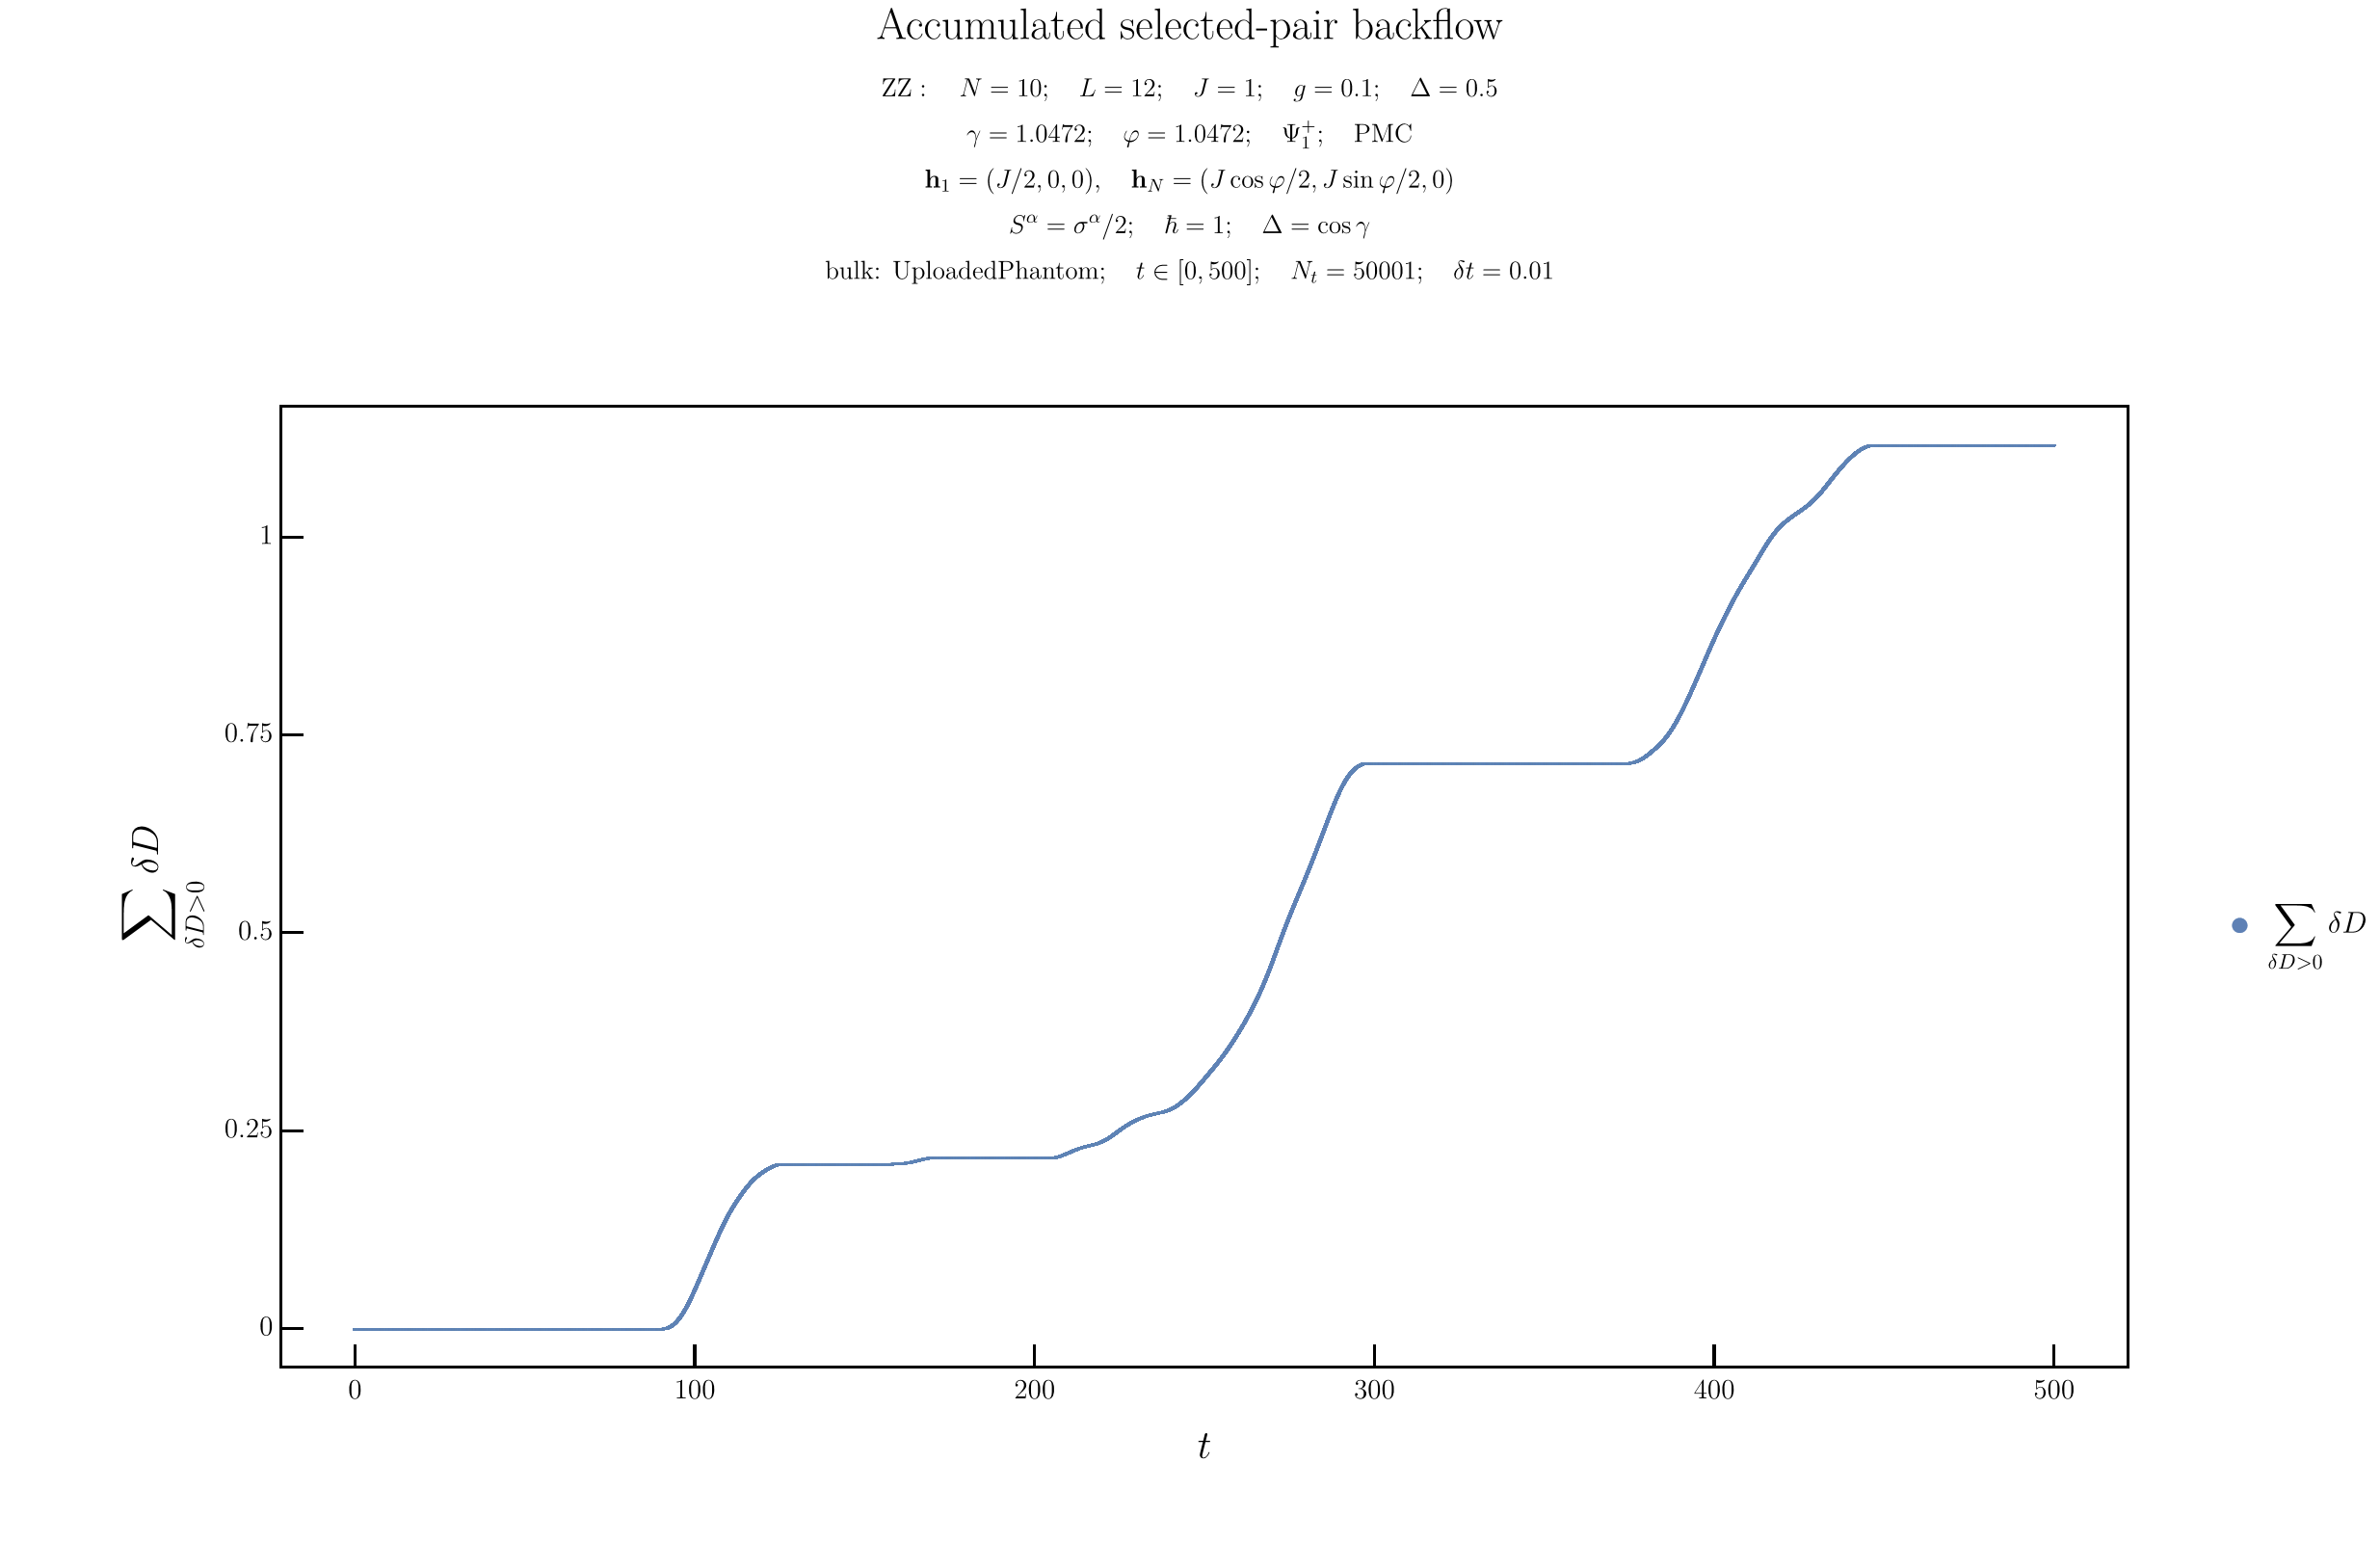
\includegraphics[width=\linewidth,height=0.49\textheight,keepaspectratio]{Phantom_ZZ_N10/Channel_BLPAccumulated.png}
\end{column}
\end{columns}
\vspace{-4pt}
\[
D(t)=\tfrac12\bigl\lVert\Lambda_t(\ket{++}\bra{++}-\ket{+-}\bra{+-})\bigr\rVert_1,\qquad
\mathcal N(t)=\sum_{t_j\le t}\max(0,\Delta D_j).
\]
\vspace{-6pt}
\begin{itemize}\setlength\itemsep{2pt}
\item \textbf{Broad backflow episodes:} $D(t)$ rises on $[90.4,126.0]$ ($+0.208$), $[204.7,297.9]$ ($+0.499$), and $[374.2,447.3]$ ($+0.402$), accumulating $\mathcal N(500)=1.117$ while $\Lambda_t$ is CPTP at all times.
\item \textbf{No step at $t=222.60$:} $t=222.60$ sits smoothly inside the slow rise over $[204.7,297.9]$.
\item \textbf{BLP vs.\ RHP:} both witness non-Markovianity, but BLP tracks broad recoherence in $\Gamma(t)$ whereas RHP tracks near-singularities of $\Lambda_t^{-1}$.
\end{itemize}
\end{frame}

% ==============================================================
\section{Part D: Synthesis}
% ==============================================================

\begin{frame}{What spikes and what does not at $t \approx 222.6$}
\footnotesize
\begin{columns}[T,totalwidth=\textwidth]
\begin{column}{0.48\textwidth}
\textbf{Spikes sharply (built from $\Lambda_t^{-1}$ / division by $\Gamma_{ab}$):}
\begin{itemize}\setlength\itemsep{3pt}
\item Canonical rates: $\gamma_{15}=+9.57$ ($222.58$), $\gamma_1=-9.69$ ($222.63$).
\item Minimum rate $\min_k\gamma_k$: $-9.69$.
\item Instantaneous RHP $g_{\mathrm{RHP}}$: $4.84$.
\item Finite-step RHP rate $r_k=w_k/\delta t$: $4.89$ ($w_k=0.0489$).
\end{itemize}
\smallskip
\textbf{Dips smoothly to near-zero:}
\begin{itemize}\setlength\itemsep{2pt}
\item $\sigma_{\min}(\St)=\lvert\Gamma_{01,10}\rvert=1.07\times 10^{-4}$ at $t=222.60$ ($\lvert\rho_{01,10}\rvert=2.7\times 10^{-5}$).
\end{itemize}
\end{column}
\begin{column}{0.49\textwidth}
\textbf{Completely smooth through $t\approx 222.6$:}
\begin{itemize}\setlength\itemsep{3pt}
\item Entropies $S_A,S_B,S_{AB}$, purities, mutual information $I(A:B)$.
\item Concurrence and negativity ($0$ there; peak is at $t\approx 298$).
\item All local Bloch components $\langle\sigma_{A,B}^\alpha\rangle$ and two-point $C_{\alpha\beta}$.
\item Choi eigenvalues, Choi negativity, map entropy, covariance errors.
\item BLP distance $D(t)$, accumulated $\mathcal N(t)$, and return overlaps.
\end{itemize}
\end{column}
\end{columns}
\smallskip
\[
\dot\rho_{ab}(t)=\underbrace{\bigl(\dot\Gamma_{ab}/\Gamma_{ab}\bigr)}_{\text{spikes}}\;\underbrace{\rho_{ab}(t)}_{\text{dips to }10^{-4}}=\dot\Gamma_{ab}(t)\,r_{ab}\quad\bigl(\text{smooth, }\lvert\dot\Gamma_{ab}\rvert\le g\bigr).
\]
\end{frame}

% ==============================================================
\begin{frame}{Zoom across the near-zero ($t \in [200, 245]$)}
\begin{columns}[T,totalwidth=\textwidth]
\begin{column}{0.59\textwidth}
\centering
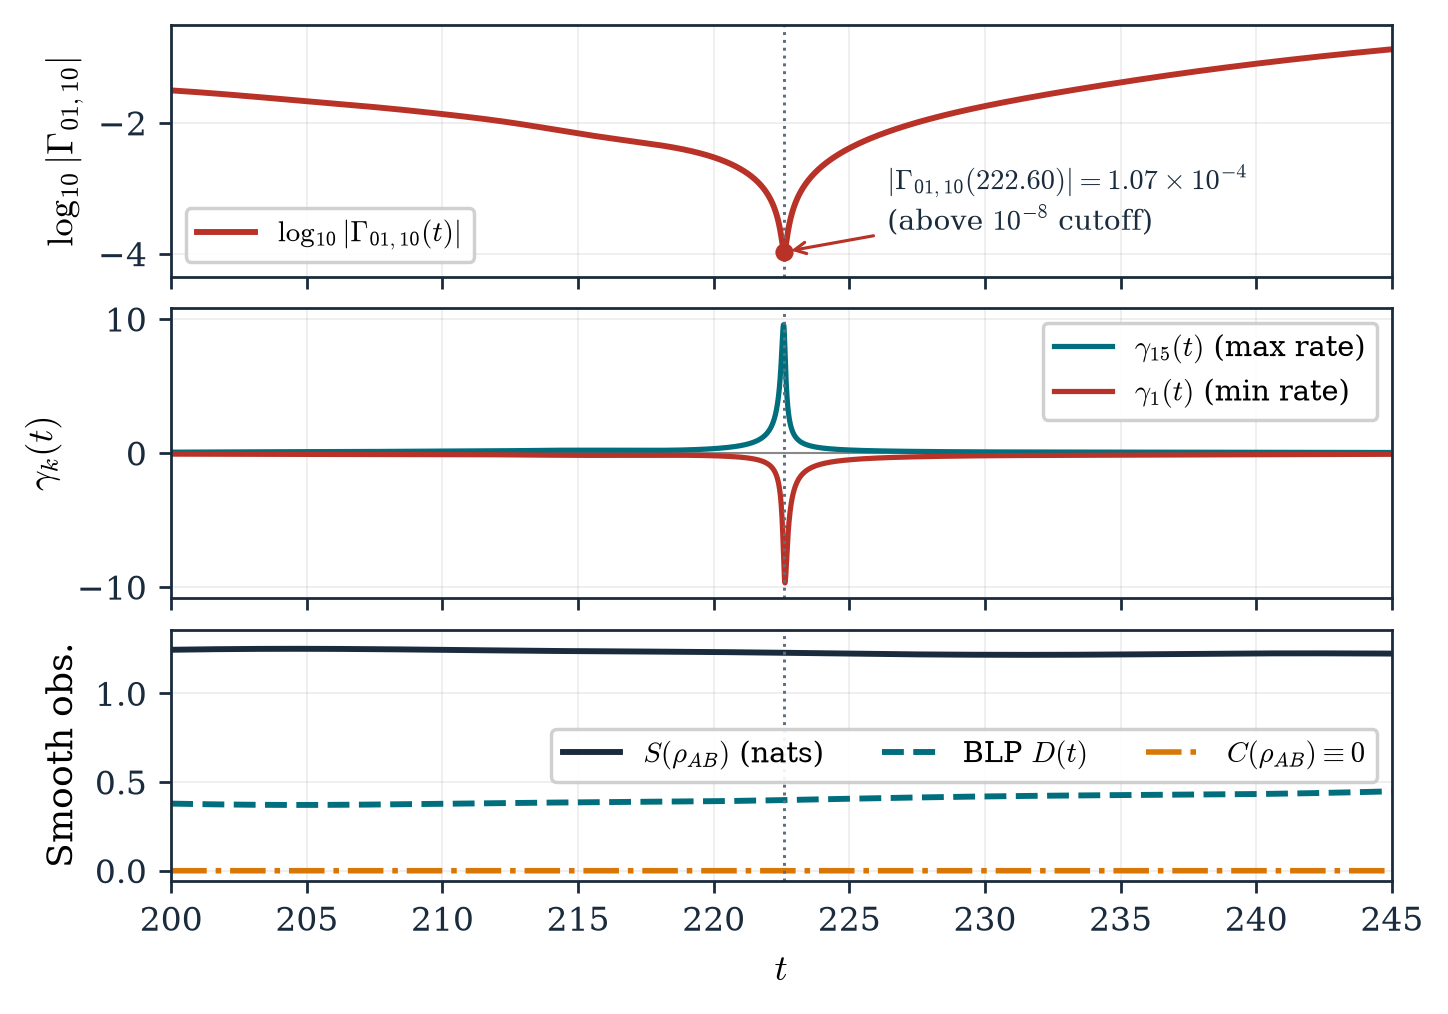
\includegraphics[width=\linewidth,height=0.80\textheight,keepaspectratio]{Phantom_ZZ_N10/new/zoom_222.png}
\end{column}
\begin{column}{0.39\textwidth}
\footnotesize
\[
t_0 = 222.60,\quad \lvert\Gamma_{01,10}(t_0)\rvert = 1.07\times 10^{-4}.
\]
\begin{itemize}\setlength\itemsep{5pt}
\item \textbf{Top:} $\lvert\Gamma_{01,10}(t)\rvert$ approaches zero smoothly to $1.07\times 10^{-4}$, staying $4$ decades above the $10^{-8}$ threshold.
\item \textbf{Middle:} logarithmic derivative $\dot\Gamma_{01,10}/\Gamma_{01,10}$ produces the antisymmetric positive/negative lobes of $\gamma_{15}$ and $\gamma_1$, whose integrals cancel in net damping.
\item \textbf{Bottom:} state functions $S(\rho_{AB})$, $C(\rho_{AB})\equiv 0$, and BLP $D(t)$ pass across $t_0$ without any feature.
\end{itemize}
\end{column}
\end{columns}
\end{frame}

% ==============================================================
\begin{frame}{Summary and open questions}
\small
\begin{itemize}\setlength\itemsep{5pt}
\item \textbf{$\Gamma(t)$ governs the run:} with $\rho_{AB}(0)=\ket{++}\bra{++}$, $\rho_{AB}(t)=\Gamma(t)/4$, and $\mathcal R\mathcal F$ symmetry reduces $\Gamma(t)$ to $4$ independent overlaps ($7$ real functions), with edge entanglement peaking at $C=0.118$ around $t=298.2$.
\item \textbf{Longitudinal sector frozen:} $[H,s_A^z]=[H,s_B^z]=0$ fixes edge populations, $z$-magnetizations, $zz$ correlations, and boundary spin currents identically, even though transverse end fields break bulk $M_z$.
\item \textbf{Only $\Lambda_t^{-1}$ spikes:} at $t=222.60$, $\lvert\Gamma_{01,10}\rvert=1.07\times 10^{-4}$ creates tall finite spikes in $\gamma_{1,15}$ and RHP witnesses while every observable of $\rho_{AB}(t)$ and $\Lambda_t$ (including BLP) stays smooth and $\Lambda_t$ stays CPTP.
\item \textbf{Origin and open questions:} $8$-fold degeneracy of the helix level allows $O(1)$ conditional rotations of $\ket{\phi_a(t)}$; ongoing questions include conditions for exact zeros vs.\ near-zeros, quantitative $d=8$ theory, and a direct comparison run with an isolated eigenstate of the same $H_M$.
\end{itemize}
\end{frame}

% ==============================================================
\begin{frame}[plain]
\end{frame}

% ==============================================================
\appendix
\section{Appendix}
% ==============================================================

\begin{frame}{Appendix 1a: Full plot inventory --- \texttt{Channel\_*} ($33$ PNGs)}
\scriptsize\setlength{\tabcolsep}{3pt}
\begin{columns}[T,totalwidth=\textwidth]
\begin{column}{0.49\textwidth}
\begin{tabular}{@{}ll@{}}
\toprule
Filename (\texttt{Channel\_*.png}) & Slide / reason \\\midrule
\texttt{BLPAccumulated} & Used: Slide C16 \\
\texttt{BLPDistance} & Used: Slide C16 \\
\texttt{CanonicalRates} & Used: Slide C14 \\
\texttt{ChoiEigenvalues} & Used: Slide C11 \\
\texttt{ChoiNegativity} & Used: Slide C12 \\
\texttt{ChoiPTMinimum} & Dup.: $-\frac14\max_{a<b}\lvert\Gamma_{ab}\rvert$ \\
\texttt{ChoiTraceError} & Check ($2.8\cdot 10^{-14}$, B3) \\
\texttt{DephasingPopulationError} & Const.\ $0$ (B2) \\
\texttt{DoubleQuantumAbs} & Dup.: $\lvert\Gamma_{00,11}\rvert$ in C1 \\
\texttt{DoubleQuantumImag} & Const.\ $0$ (C2) \\
\texttt{DoubleQuantumReal} & Dup.: $\operatorname{Re}\Gamma_{00,11}$ (App.\ 2c) \\
\texttt{EntanglingConcurrence} & Dup.: $\equiv$ \texttt{Concurrence} (B1) \\
\texttt{FlipCovarianceError} & Dup.: $\equiv$ \texttt{Refl.Cov.} (App.\ 2c) \\
\texttt{Gamma\_Abs} & Used: Slide C1 \\
\texttt{Gamma\_Im} & Used: Slide C2 \\
\texttt{Gamma\_Re} & Used: Slide C2 \\
\texttt{KrausRank} & Const.\ $4$ for $t\ge 0.13$ (B2) \\\bottomrule
\end{tabular}
\end{column}
\begin{column}{0.49\textwidth}
\begin{tabular}{@{}ll@{}}
\toprule
Filename (\texttt{Channel\_*.png}) & Slide / reason \\\midrule
\texttt{MapEntropy} & Dup.: $\equiv$ \texttt{EntropyAB} (B1) \\
\texttt{MinChoiEigenvalue} & Check ($-3.3\cdot 10^{-15}$, B3) \\
\texttt{MinDephasingEigenvalue} & Dup.: $4\lambda_{\min}$ (B1) \\
\texttt{MinimumRate} & Dup.: $\gamma_1(t)$ (App.\ 2c) \\
\texttt{MinSingularValue} & Used: Slide C13 \\
\texttt{MixedInputEntropy} & Const.\ $\ln 4$ (B2) \\
\texttt{ReflectionCovarianceError} & Used: C3 \\
\texttt{RetentionA} & Const.\ $1$ ($s_A^z$ cons., B2) \\
\texttt{RFCovarianceError} & Used: Slide C3 \\
\texttt{RHPFiniteStep} & Used: Slide C15 \\
\texttt{RHPFiniteStepRate} & Dup.: $w_k/\delta t$ (App.\ 2c) \\
\texttt{RHPInstantaneous} & Used: Slide C15 \\
\texttt{SignalAtoB} & Const.\ $0$ (B2) \\
\texttt{TPError} & Check ($4.6\cdot 10^{-14}$, B3) \\
\texttt{U1CovarianceError} & Const.\ $0$ (diag.\ $\St$, B2) \\
\texttt{UnitalityError} & Const.\ $0$ (Schur map, B2) \\\bottomrule
\end{tabular}
\end{column}
\end{columns}
\end{frame}

% ==============================================================
\begin{frame}{Appendix 1b: Full plot inventory --- \texttt{State\_*} ($50$ PNGs, part I)}
\scriptsize\setlength{\tabcolsep}{3pt}
\begin{columns}[T,totalwidth=\textwidth]
\begin{column}{0.49\textwidth}
\begin{tabular}{@{}ll@{}}
\toprule
Filename (\texttt{State\_*.png}) & Slide / reason \\\midrule
\texttt{Concurrence} & Used: Slide C9 \\
\texttt{ConnectedXX} & Dup.: $C_{xx}-\langle\sigma_A^x\rangle^2$ \\
\texttt{ConnectedXY} & Dup.: $C_{xy}^c$ (from C5, C8) \\
\texttt{ConnectedXZ} & Dup.: $\equiv$ \texttt{CorrelationXZ} \\
\texttt{ConnectedYX} & Dup.: $-\texttt{ConnectedXY}$ ($\mathcal R\mathcal F$) \\
\texttt{ConnectedYY} & Dup.: $C_{yy}+\langle\sigma_A^y\rangle^2$ \\
\texttt{ConnectedYZ} & Dup.: $\equiv$ \texttt{CorrelationYZ} \\
\texttt{ConnectedZX} & Dup.: $-\texttt{CorrelationXZ}$ ($\mathcal R\mathcal F$) \\
\texttt{ConnectedZY} & Dup.: $+\texttt{CorrelationYZ}$ ($\mathcal R\mathcal F$) \\
\texttt{ConnectedZZ} & Const.\ $0$ (frozen pop., B2) \\
\texttt{CorrelationXX} & Used: Slide C8 \\
\texttt{CorrelationXY} & Derived (C8) \\
\texttt{CorrelationXZ} & Used: App.\ 2d (cited C8) \\\bottomrule
\end{tabular}
\end{column}
\begin{column}{0.49\textwidth}
\begin{tabular}{@{}ll@{}}
\toprule
Filename (\texttt{State\_*.png}) & Slide / reason \\\midrule
\texttt{CorrelationYX} & Dup.: $-\texttt{CorrelationXY}$ ($\mathcal R\mathcal F$) \\
\texttt{CorrelationYY} & Used: Slide C8 \\
\texttt{CorrelationYZ} & Used: App.\ 2d (cited C8) \\
\texttt{CorrelationZX} & Dup.: $-\texttt{CorrelationXZ}$ ($\mathcal R\mathcal F$) \\
\texttt{CorrelationZY} & Dup.: $+\texttt{CorrelationYZ}$ ($\mathcal R\mathcal F$) \\
\texttt{CorrelationZZ} & Const.\ $0$ (frozen pop., B2) \\
\texttt{CurrentLeft} & Const.\ $0$ (B2) \\
\texttt{CurrentRight} & Const.\ $0$ (B2) \\
\texttt{EdgeCoherences\_Abs} & Used: Slide C4 \\
\texttt{EdgeCoherences\_Im} & Dup.: $\frac14\,\texttt{Gamma\_Im}$ (B1) \\
\texttt{EdgeCoherences\_Re} & Dup.: $\frac14\,\texttt{Gamma\_Re}$ (B1) \\
\texttt{EdgeDensityEigenvalues} & Dup.: $\frac14\spec\Gamma$ (2b) \\\bottomrule
\end{tabular}
\end{column}
\end{columns}
\end{frame}

% ==============================================================
\begin{frame}{Appendix 1c: Full plot inventory --- \texttt{State\_*} ($50$ PNGs, part II)}
\scriptsize\setlength{\tabcolsep}{3pt}
\begin{columns}[T,totalwidth=\textwidth]
\begin{column}{0.49\textwidth}
\begin{tabular}{@{}ll@{}}
\toprule
Filename (\texttt{State\_*.png}) & Slide / reason \\\midrule
\texttt{EdgePopulations} & Const.\ $1/4$ each (B2) \\
\texttt{EntropyA} & Used: Slide C6 \\
\texttt{EntropyAB} & Used: Slide C6 \\
\texttt{EntropyB} & Dup.: $\equiv$ \texttt{EntropyA} ($\rho_B=\rho_A^*$) \\
\texttt{FullOverlap} & Used: Slide C10 \\
\texttt{HermiticityError} & Check ($<10^{-12}$, B3) \\
\texttt{InitialOverlap} & Used: Slide C10 \\
\texttt{LocalAX} & Used: Slide C5 \\
\texttt{LocalAY} & Used: Slide C5 \\
\texttt{LocalAZ} & Const.\ $0$ (frozen pop., B2) \\
\texttt{LocalBX} & Dup.: $+\texttt{LocalAX}$ ($\rho_B=\rho_A^*$) \\
\texttt{LocalBY} & Dup.: $-\texttt{LocalAY}$ (App.\ 2b) \\
\texttt{LocalBZ} & Const.\ $0$ (frozen pop., B2) \\\bottomrule
\end{tabular}
\end{column}
\begin{column}{0.49\textwidth}
\begin{tabular}{@{}ll@{}}
\toprule
Filename (\texttt{State\_*.png}) & Slide / reason \\\midrule
\texttt{LocalCoherences\_Abs} & Dup.: $\frac12\sqrt{\langle\sigma_A^x\rangle^2+\langle\sigma_A^y\rangle^2}$ \\
\texttt{LocalCoherences\_Im} & Dup.: $-\frac12\langle\sigma_{A,B}^y\rangle$ (C5) \\
\texttt{LocalCoherences\_Re} & Dup.: $+\frac12\langle\sigma_{A,B}^x\rangle$ (C5) \\
\texttt{MagnetizationA} & Const.\ $0$ ($\equiv$ \texttt{LocalAZ}, B2) \\
\texttt{MagnetizationB} & Const.\ $0$ ($\equiv$ \texttt{LocalBZ}, B2) \\
\texttt{MinEigenvalue} & Dup.: $\lambda_4(\rho_{AB})$ (App.\ 2b) \\
\texttt{MutualInfo} & Used: Slide C7 \\
\texttt{Negativity} & Companion to C9 (App.\ 2b) \\
\texttt{Purity} & Companion to C6 (App.\ 2b) \\
\texttt{PurityA} & Companion to \texttt{EntropyA} \\
\texttt{PurityB} & Dup.: $\equiv$ \texttt{PurityA} ($\rho_B=\rho_A^*$) \\
\texttt{TraceError} & Check ($7.1\cdot 10^{-15}$, B3) \\\bottomrule
\end{tabular}
\end{column}
\end{columns}
\medskip
\mutednote{Inventory total: $33\text{ (\texttt{Channel\_*})} + 25 + 25\text{ (\texttt{State\_*})} = \mathbf{83}$ exported PNGs accounted for.}
\end{frame}

% ==============================================================
\begin{frame}{Appendix 2a: Four symmetry-independent overlaps $\Gamma_{ab}(t)$}
\begin{columns}[T,totalwidth=\textwidth]
\begin{column}{0.59\textwidth}
\centering
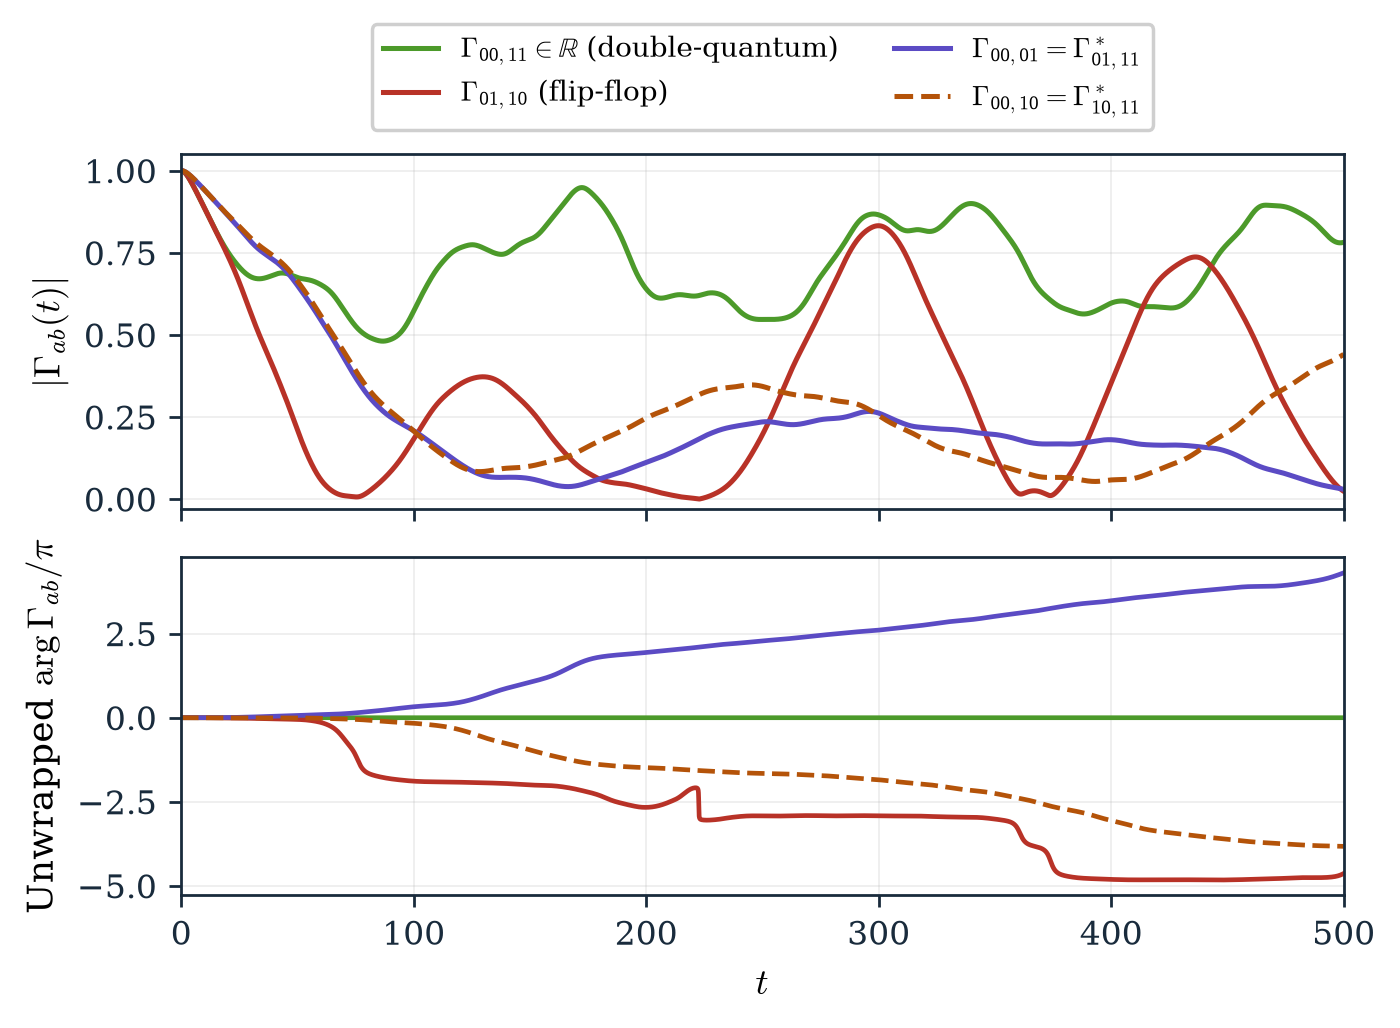
\includegraphics[width=\linewidth,height=0.80\textheight,keepaspectratio]{Phantom_ZZ_N10/new/independent_gammas.png}
\end{column}
\begin{column}{0.39\textwidth}
\footnotesize
\[
\Gamma_{00,01}=\Gamma_{01,11}^*,\ \Gamma_{00,10}=\Gamma_{10,11}^*,\ \Gamma_{00,11}\in\mathbb R
\]
\begin{itemize}\setlength\itemsep{5pt}
\item \textbf{Top:} magnitudes of the $4$ independent functions; the two single-flip pairs split apart after $t\approx 30$ ($\max_t\lvert\Gamma_{00,01}-\Gamma_{00,10}\rvert=0.413$).
\item \textbf{Bottom:} unwrapped phases $\arg\Gamma_{ab}(t)/\pi$; $\Gamma_{00,11}$ stays pinned at $0$, while $\Gamma_{01,10}$ undergoes a rapid $-\pi$ phase slip across the near-zero at $t=222.60$.
\end{itemize}
\end{column}
\end{columns}
\end{frame}

% ==============================================================
\begin{frame}{Appendix 2b: Companion and duplicate \texttt{State\_*} plots}
\centering
\begin{columns}[T,totalwidth=\textwidth]
\begin{column}{0.48\textwidth}
\centering
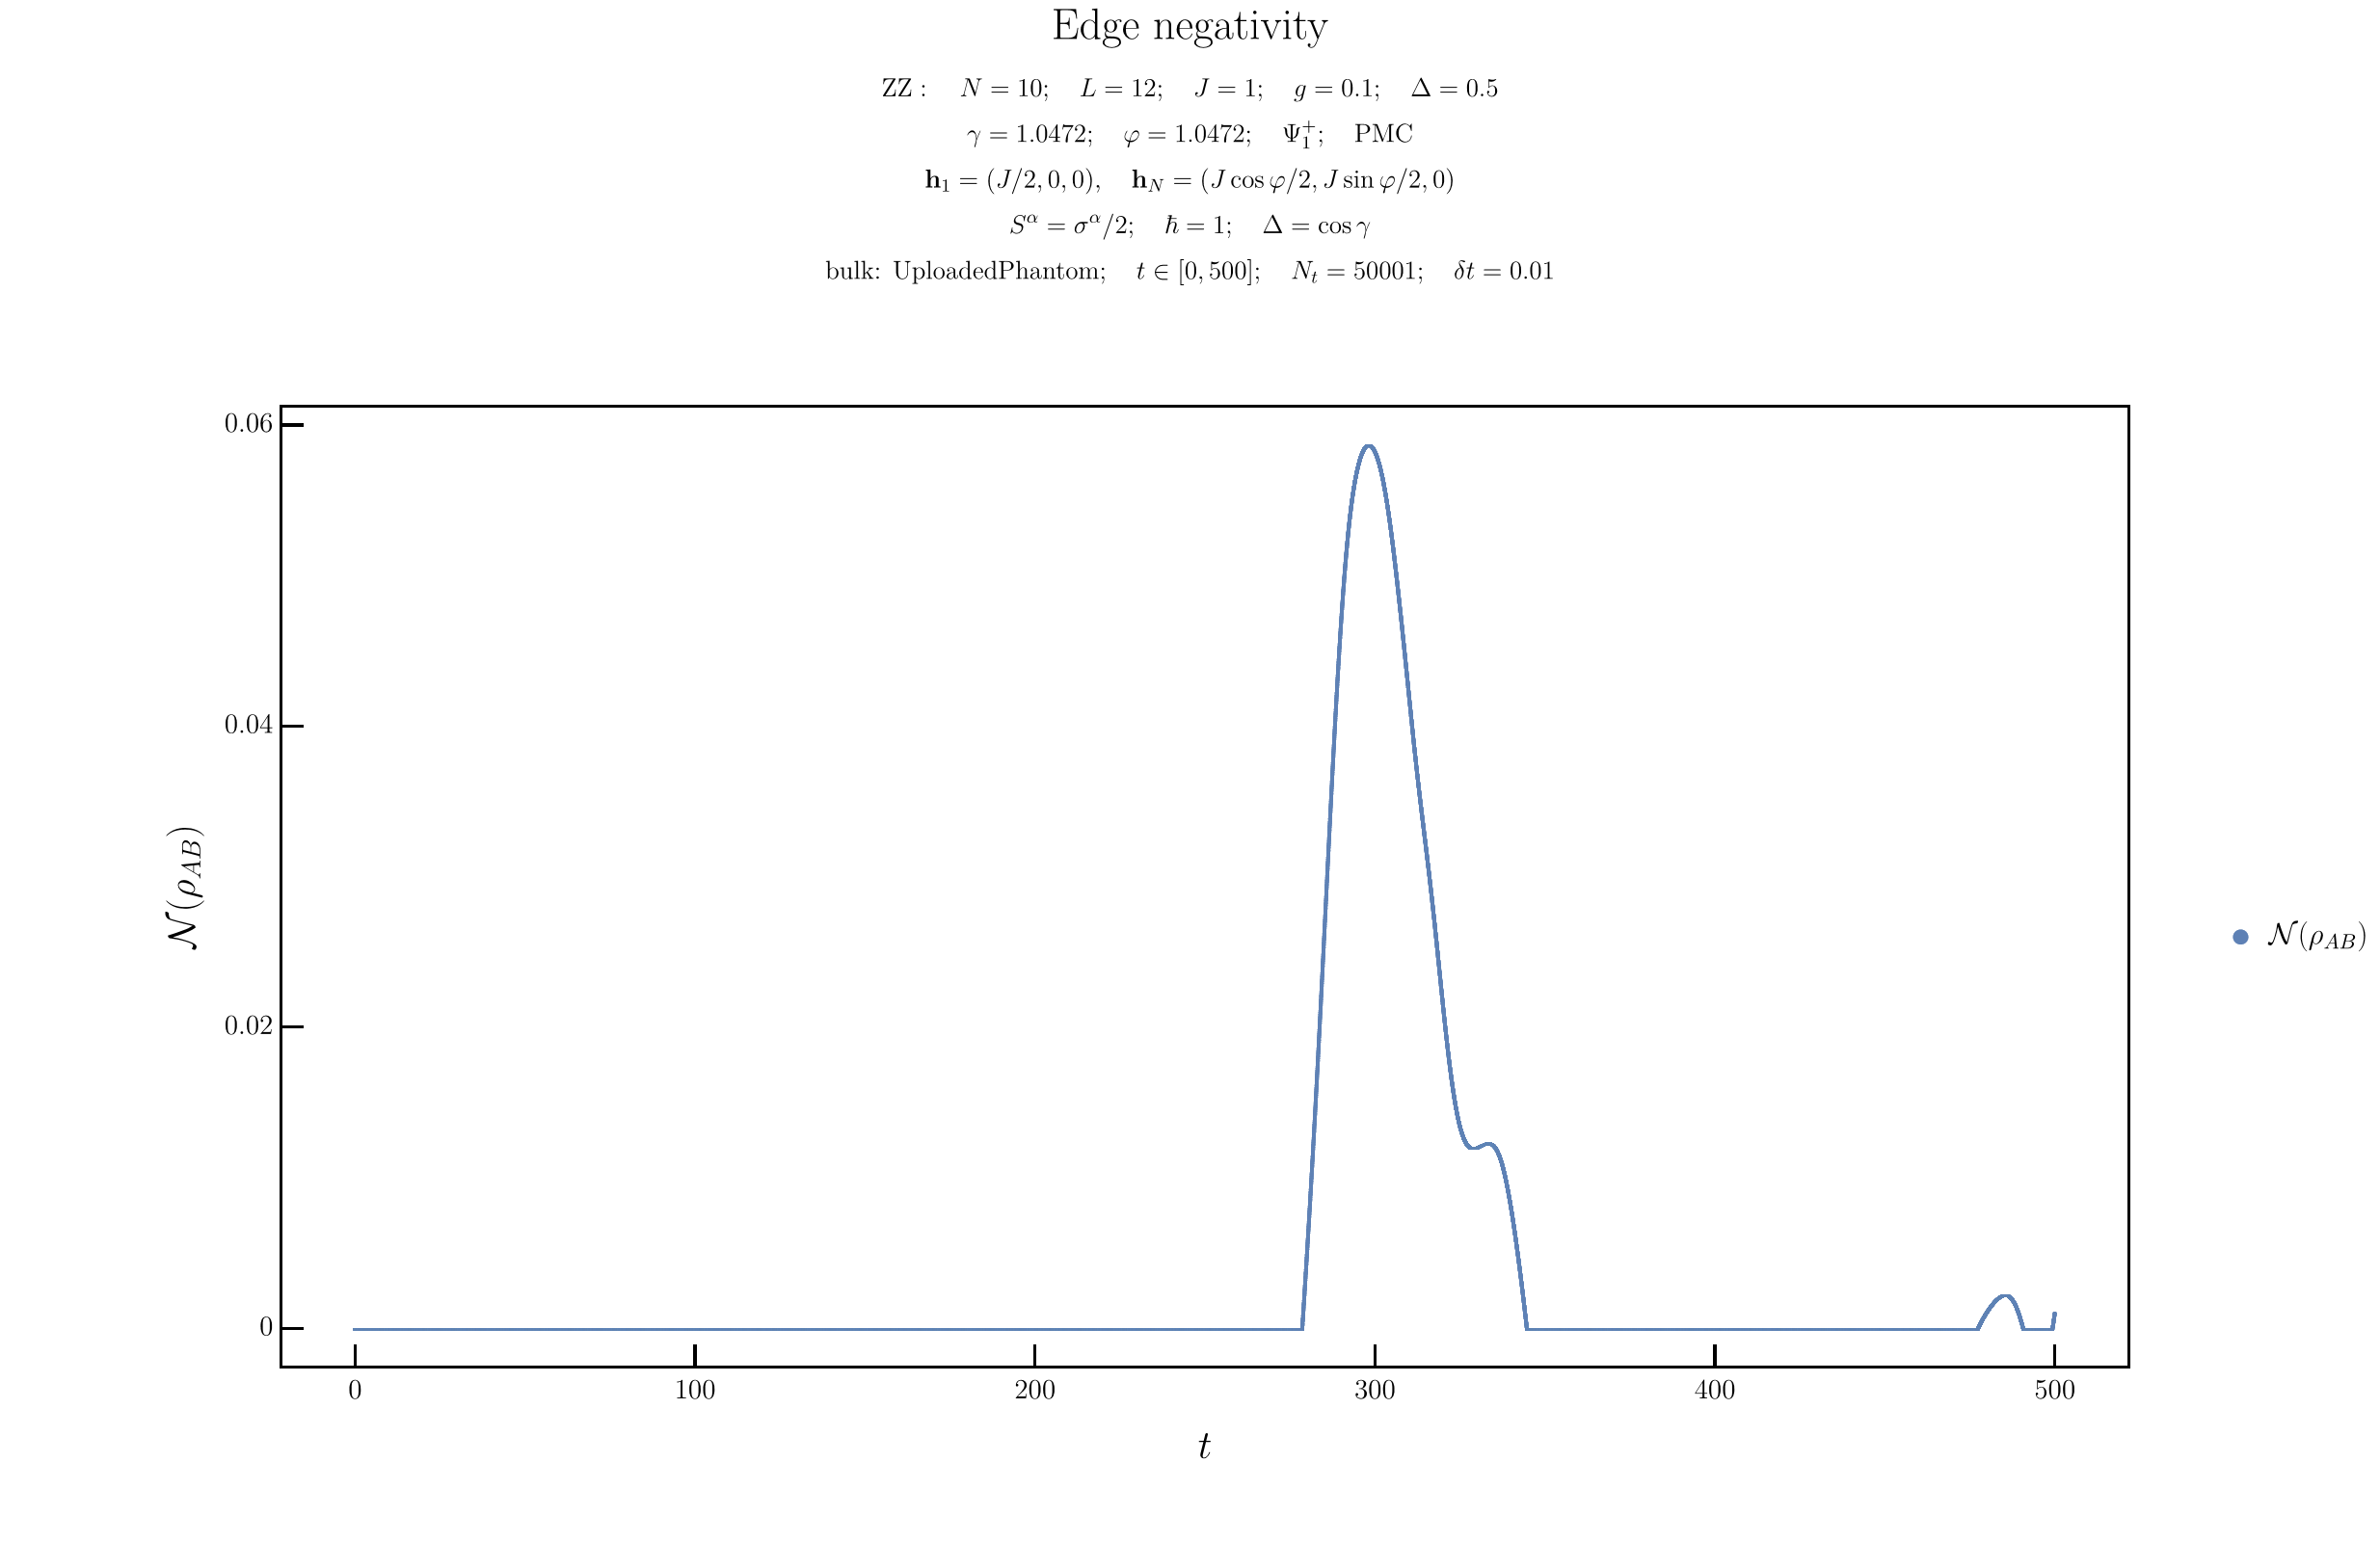
\includegraphics[width=\linewidth,height=0.36\textheight,keepaspectratio]{Phantom_ZZ_N10/State_Negativity.png}\\[3pt]
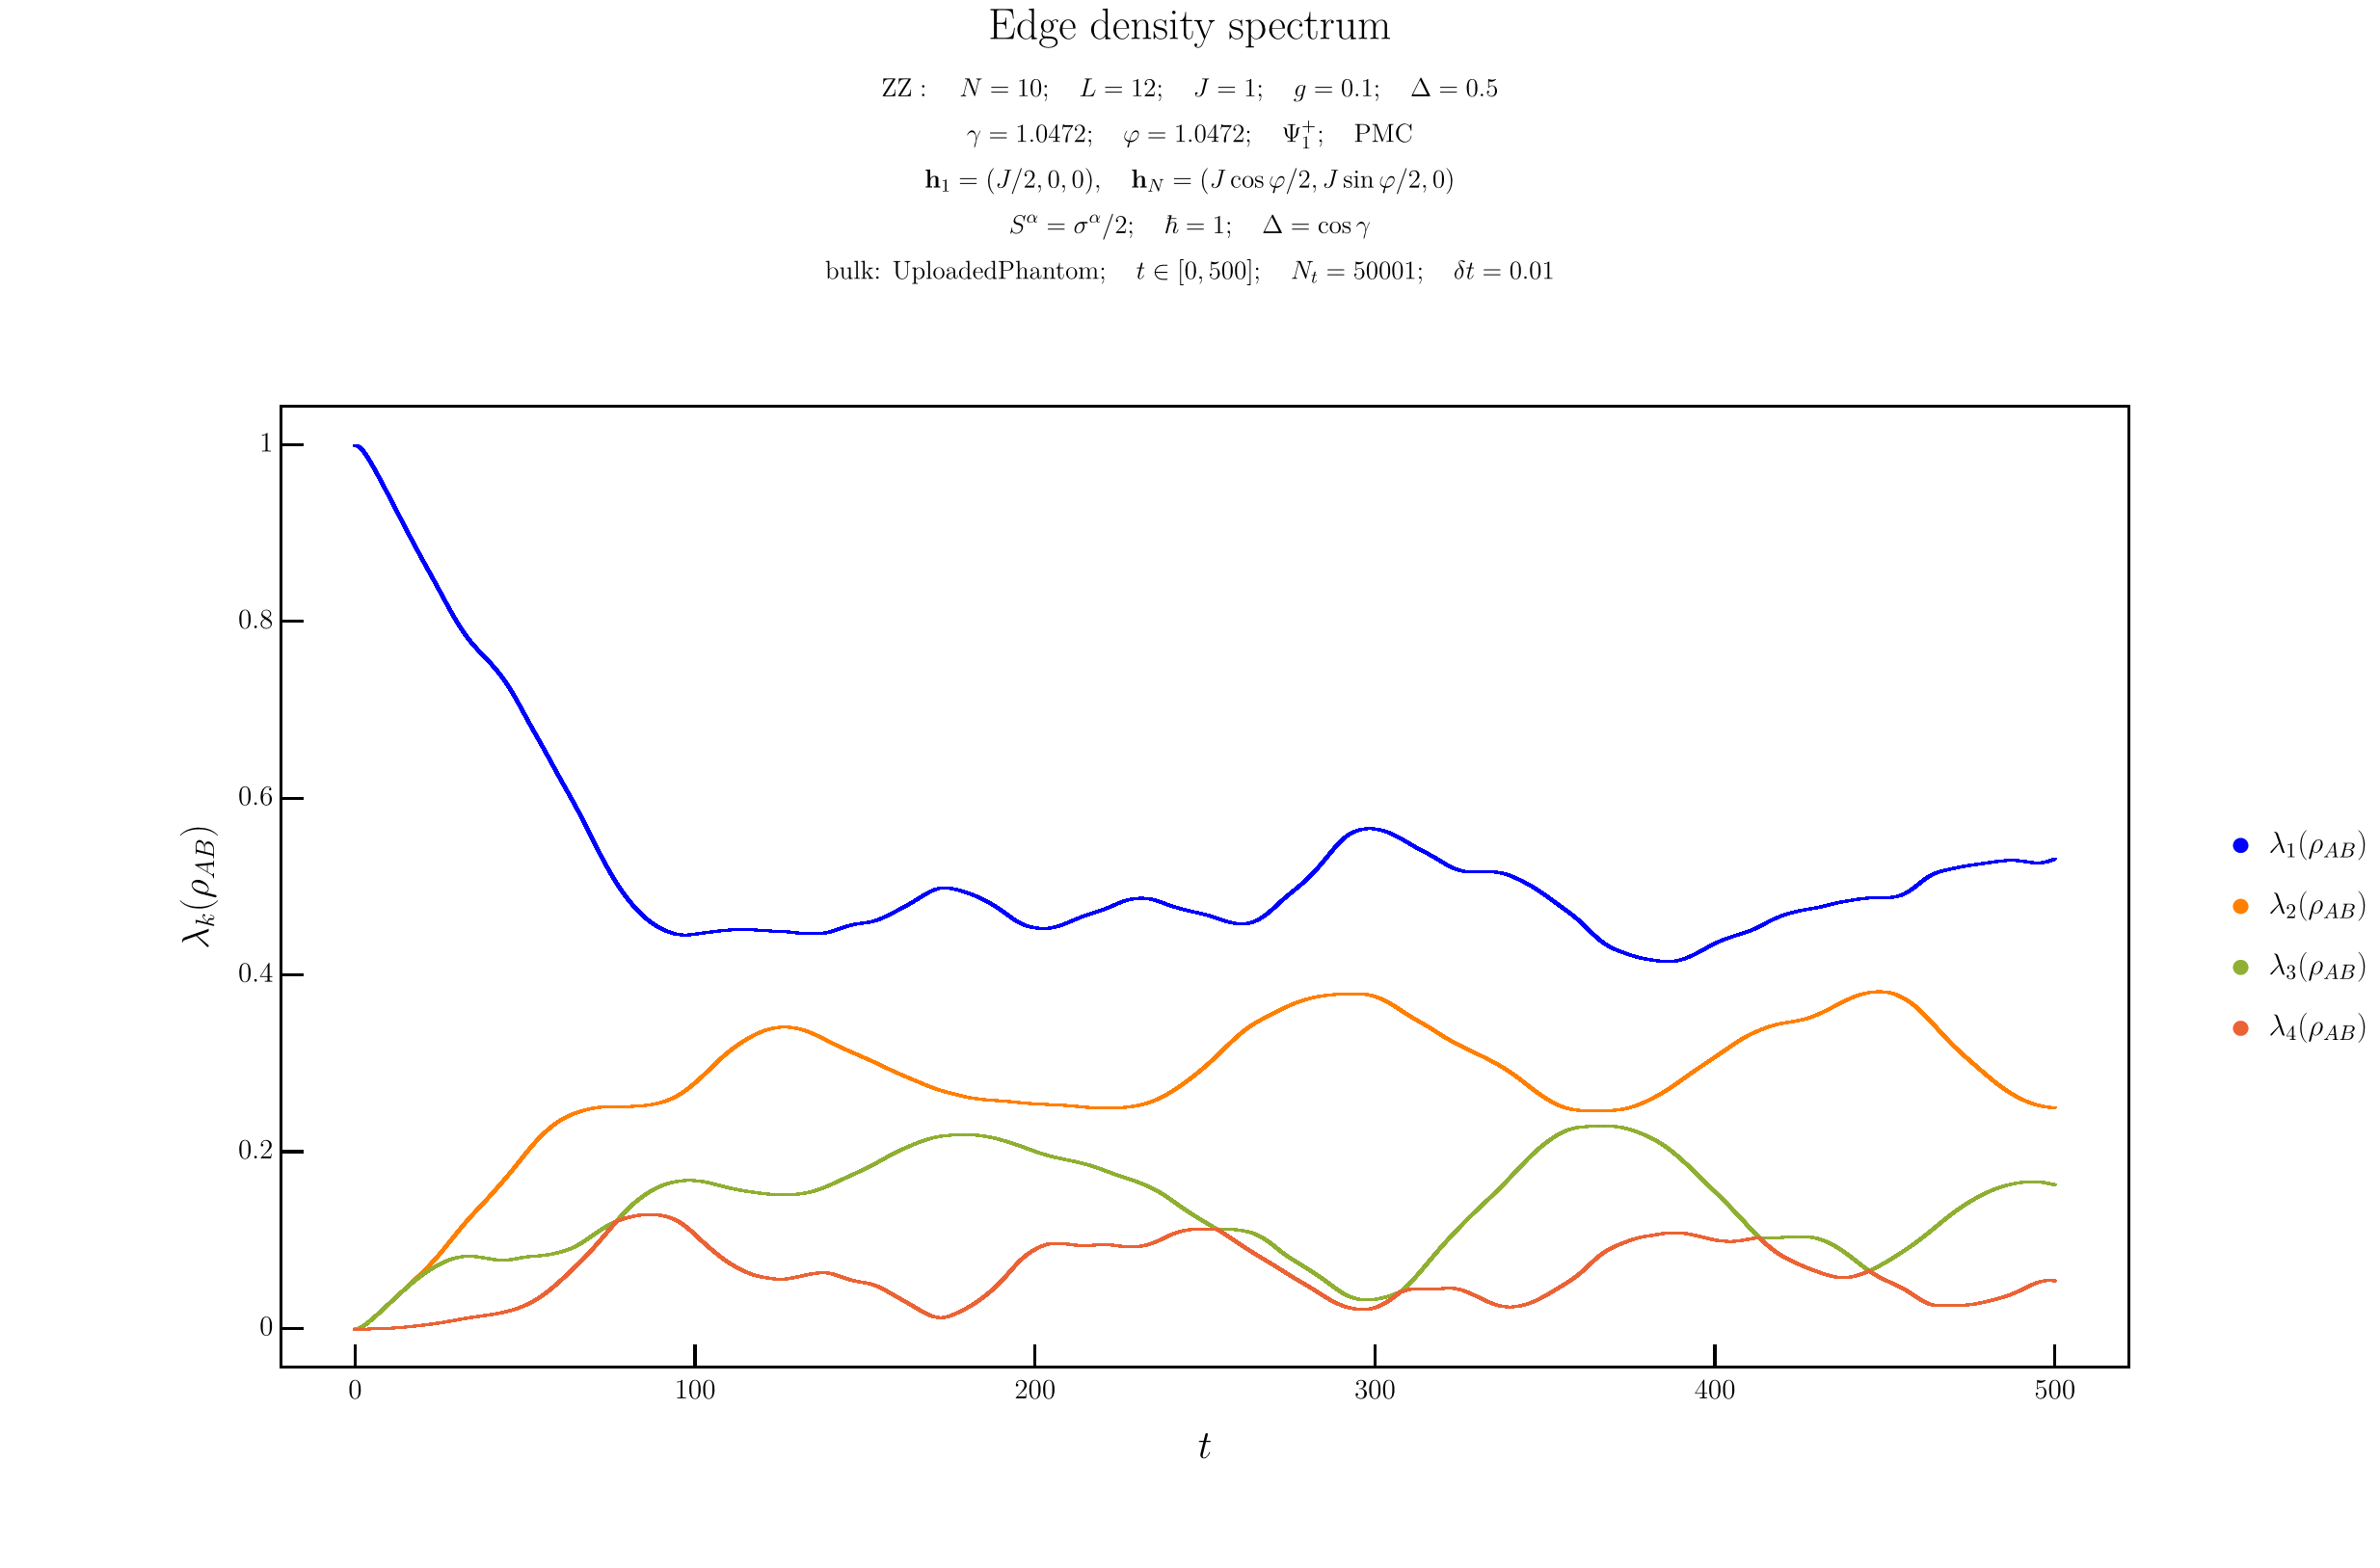
\includegraphics[width=\linewidth,height=0.36\textheight,keepaspectratio]{Phantom_ZZ_N10/State_EdgeDensityEigenvalues.png}
\end{column}
\begin{column}{0.48\textwidth}
\centering
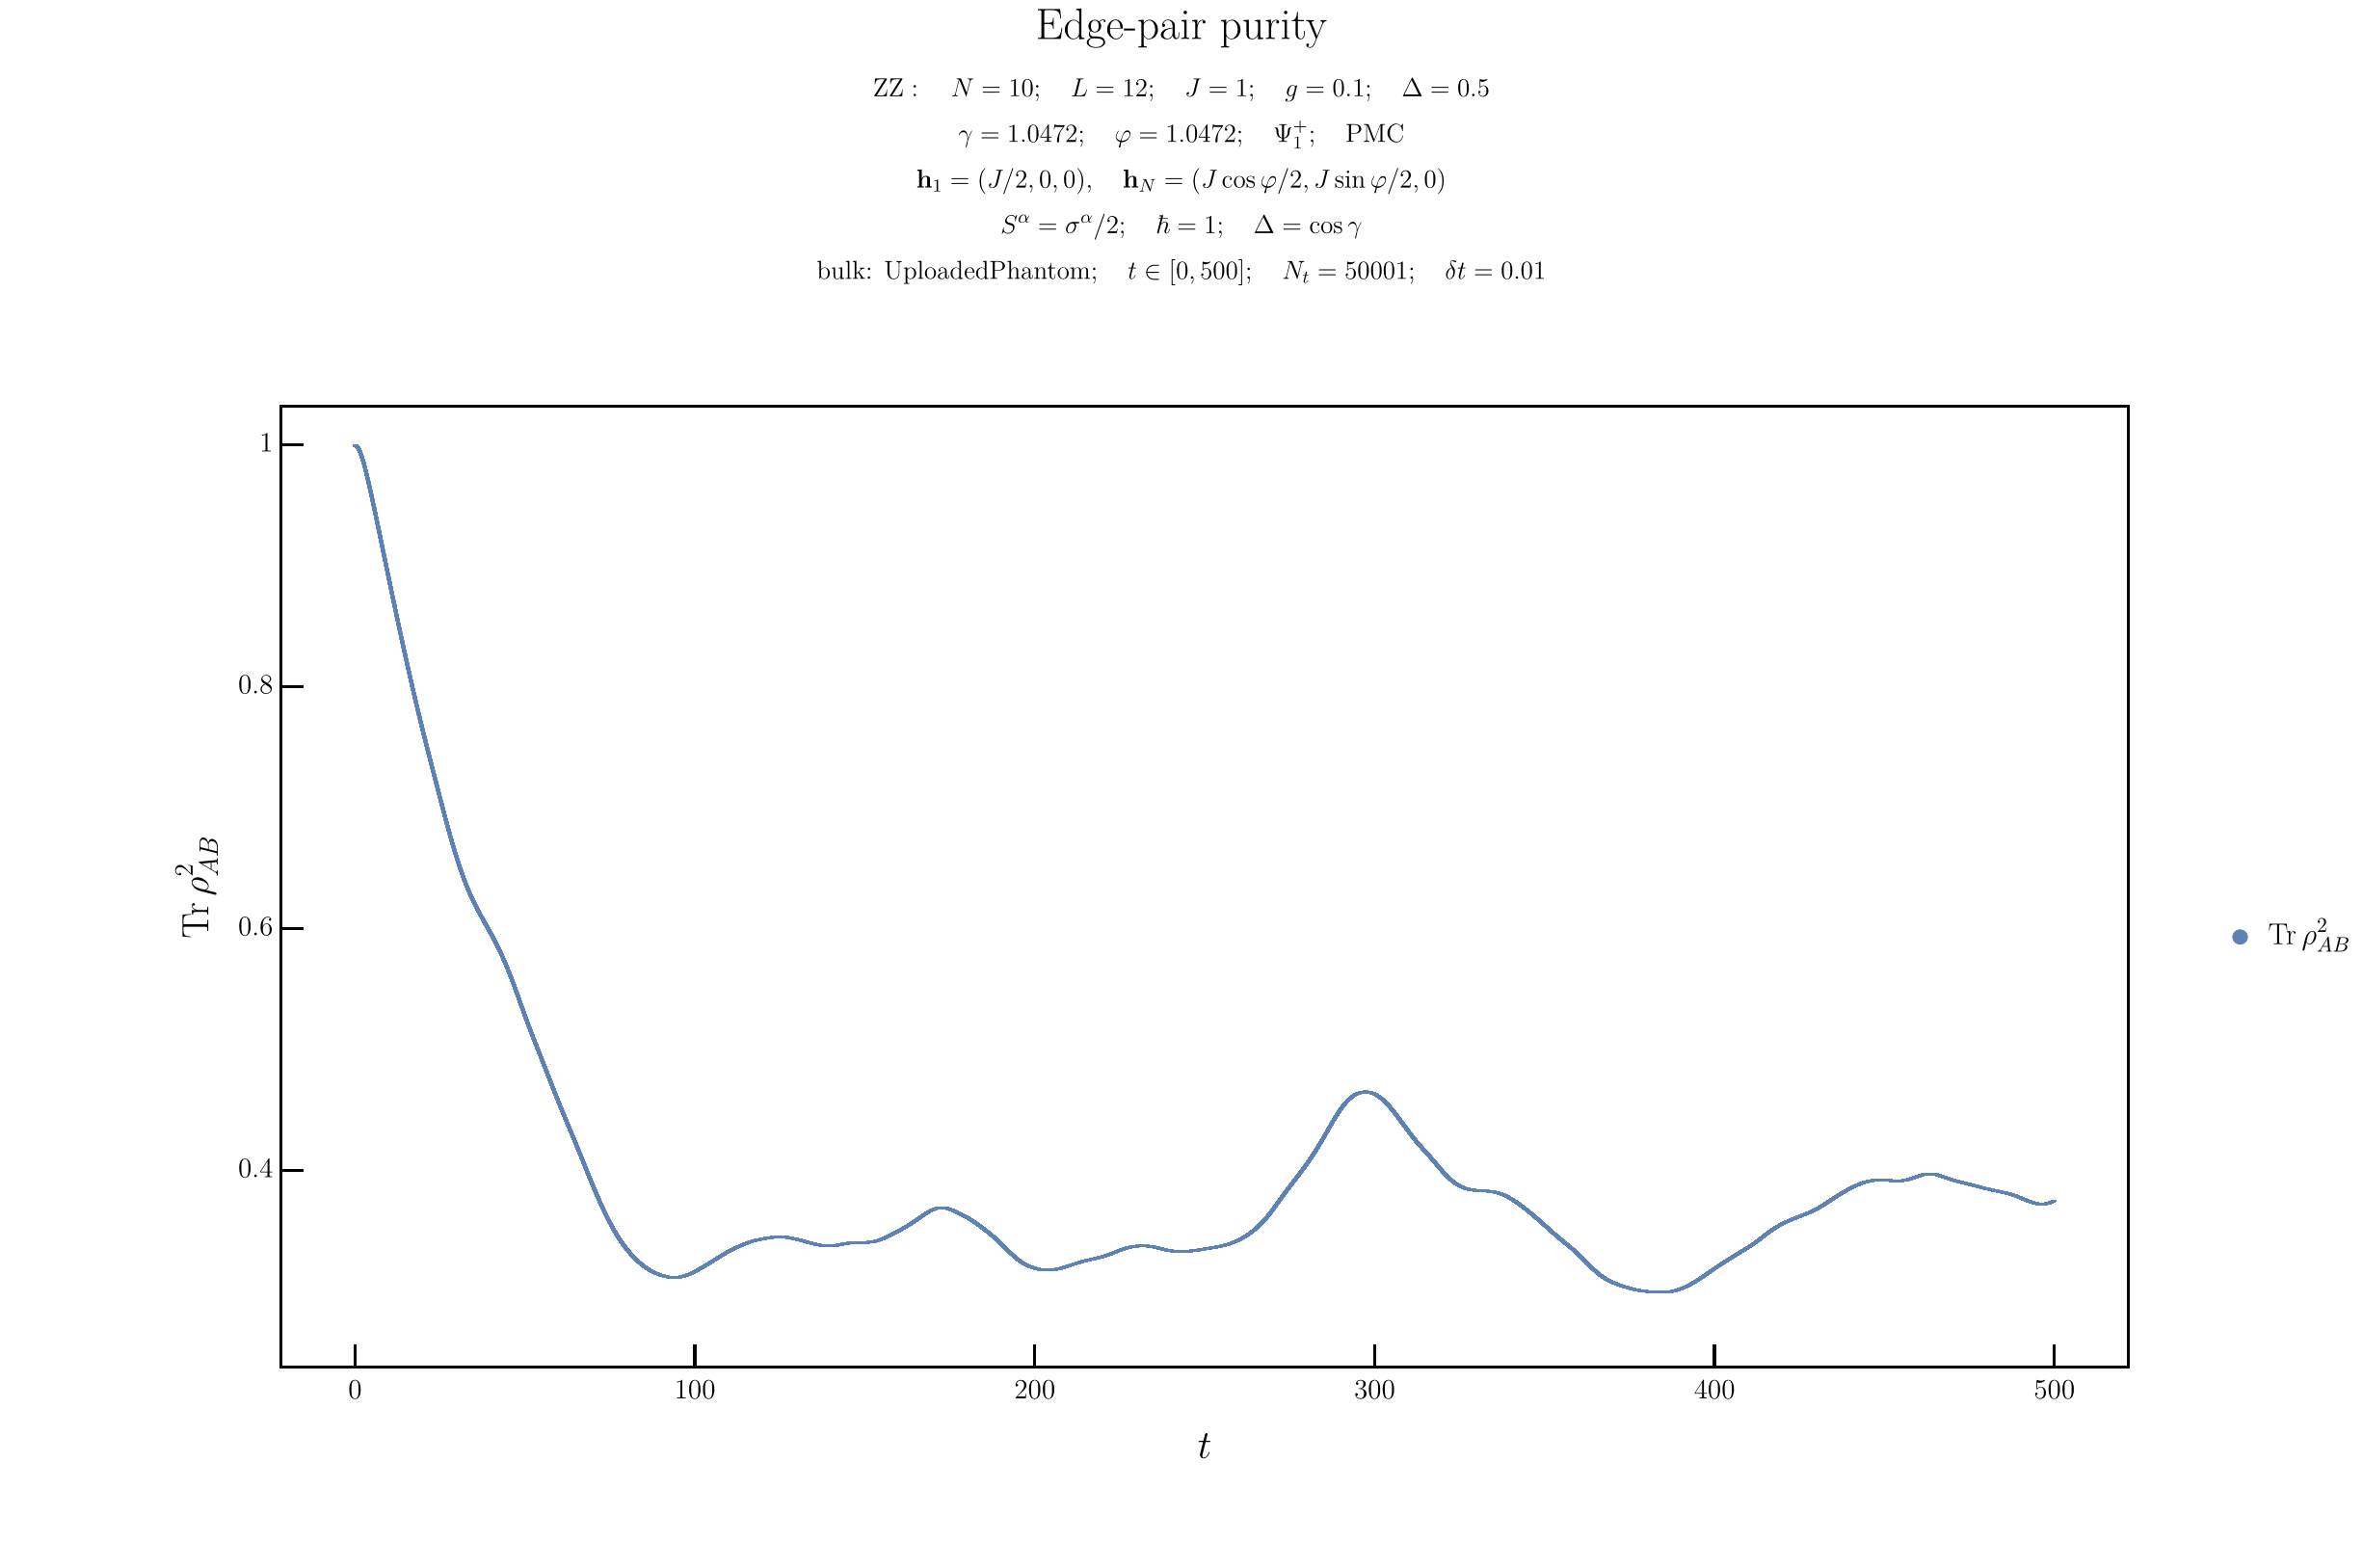
\includegraphics[width=\linewidth,height=0.36\textheight,keepaspectratio]{Phantom_ZZ_N10/State_Purity.png}\\[3pt]
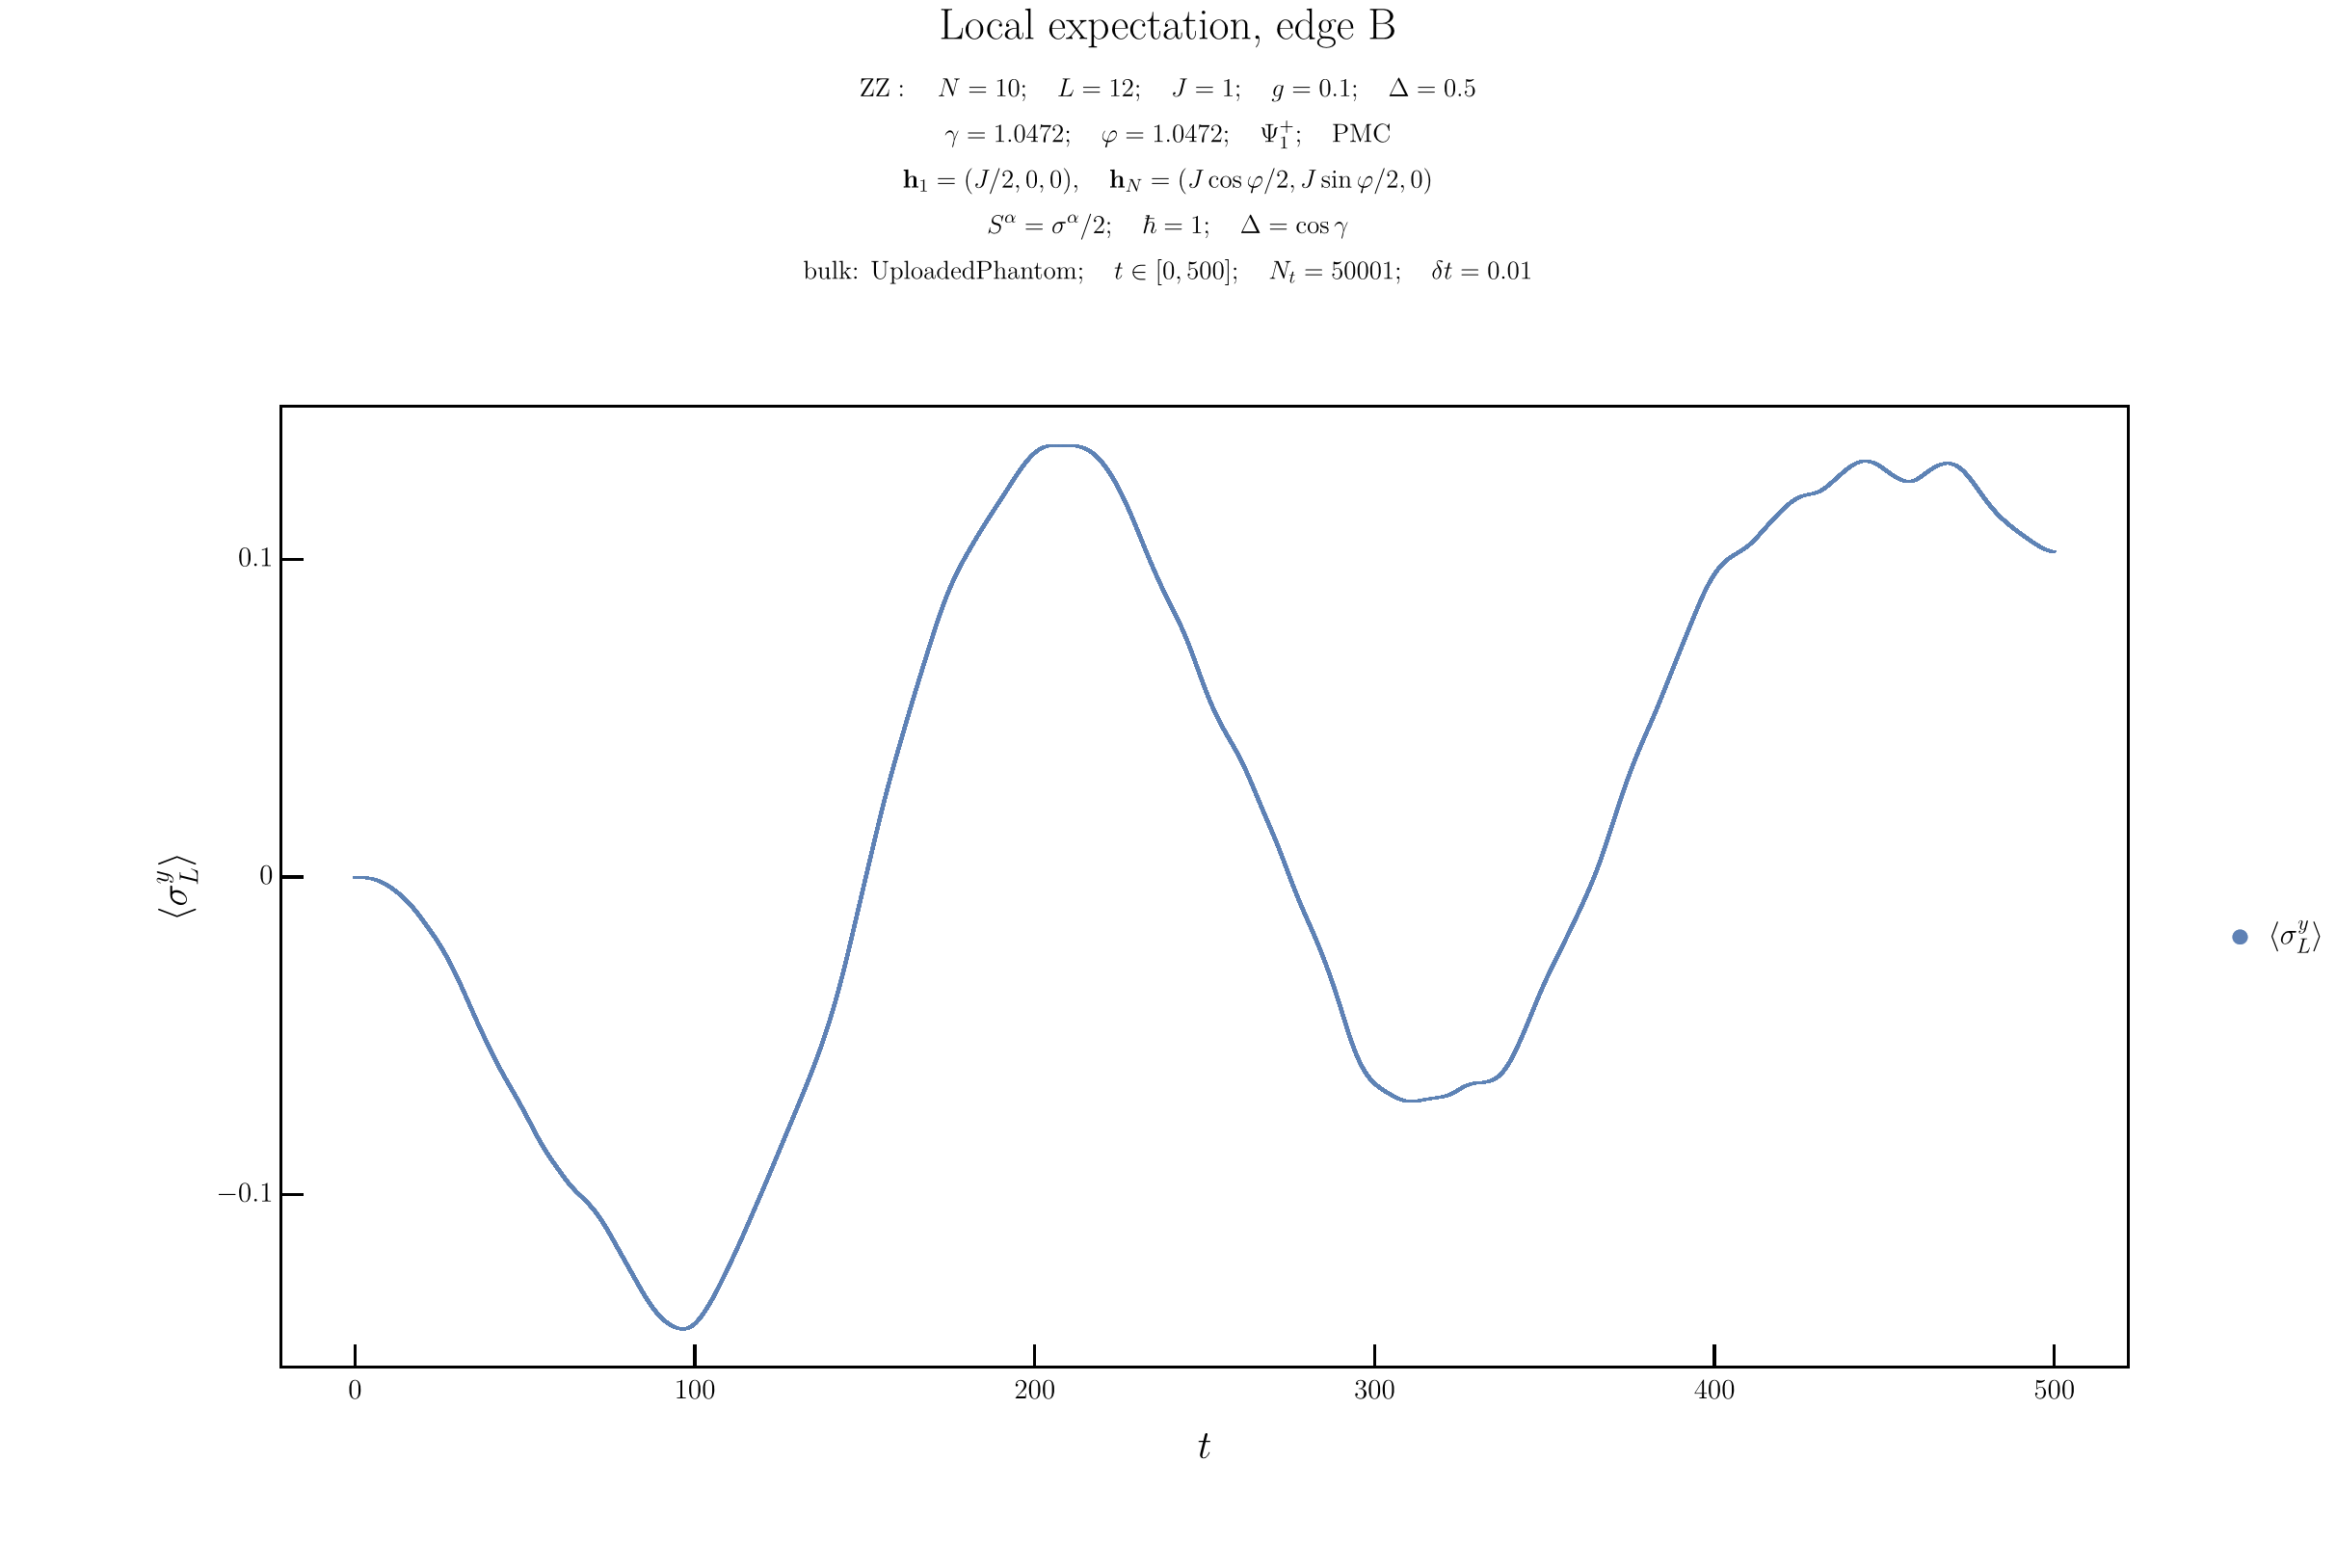
\includegraphics[width=\linewidth,height=0.36\textheight,keepaspectratio]{Phantom_ZZ_N10/State_LocalBY.png}
\end{column}
\end{columns}
\vspace{2pt}
\mutednote{Top: negativity (peak $0.0587$ at $t=298.2$) and purity $\Tr\rho_{AB}^2$. Bottom: sorted $\lambda_k(\rho_{AB})=\tfrac14\spec\Gamma$ and $\langle\sigma_B^y\rangle=-\langle\sigma_A^y\rangle$.}
\end{frame}

% ==============================================================
\begin{frame}{Appendix 2c: Companion and duplicate \texttt{Channel\_*} plots}
\centering
\begin{columns}[T,totalwidth=\textwidth]
\begin{column}{0.48\textwidth}
\centering
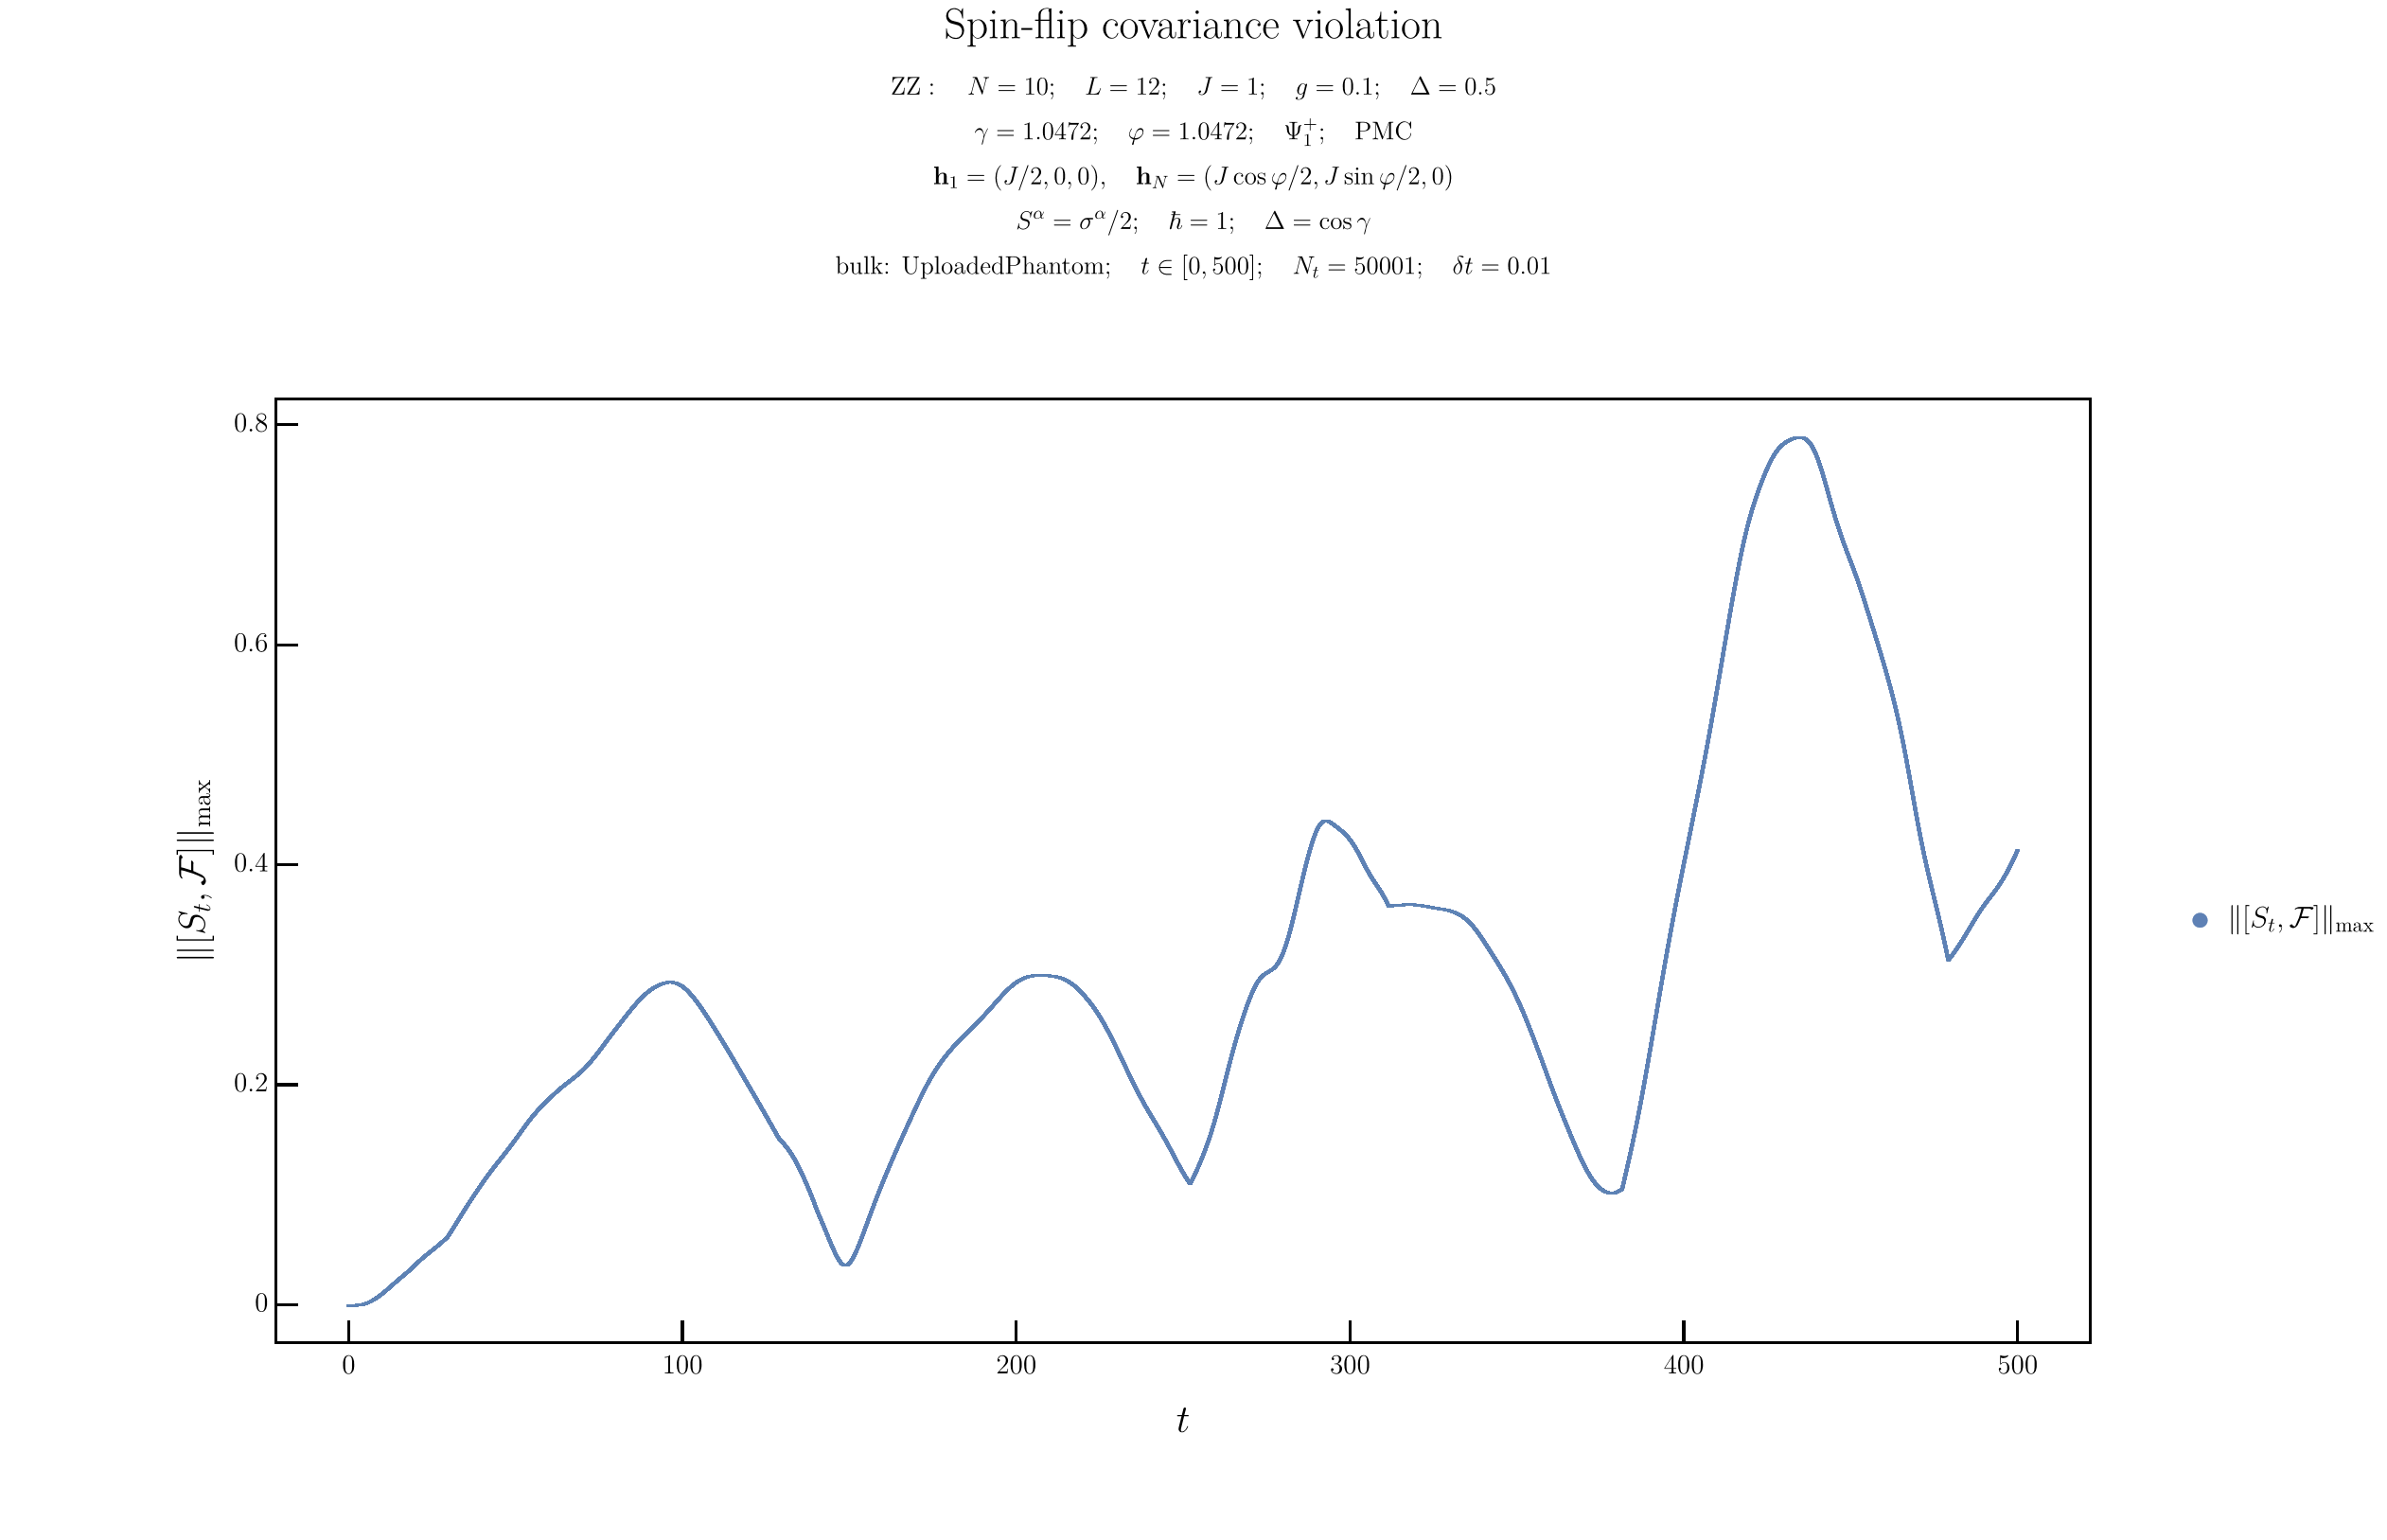
\includegraphics[width=\linewidth,height=0.36\textheight,keepaspectratio]{Phantom_ZZ_N10/Channel_FlipCovarianceError.png}\\[3pt]
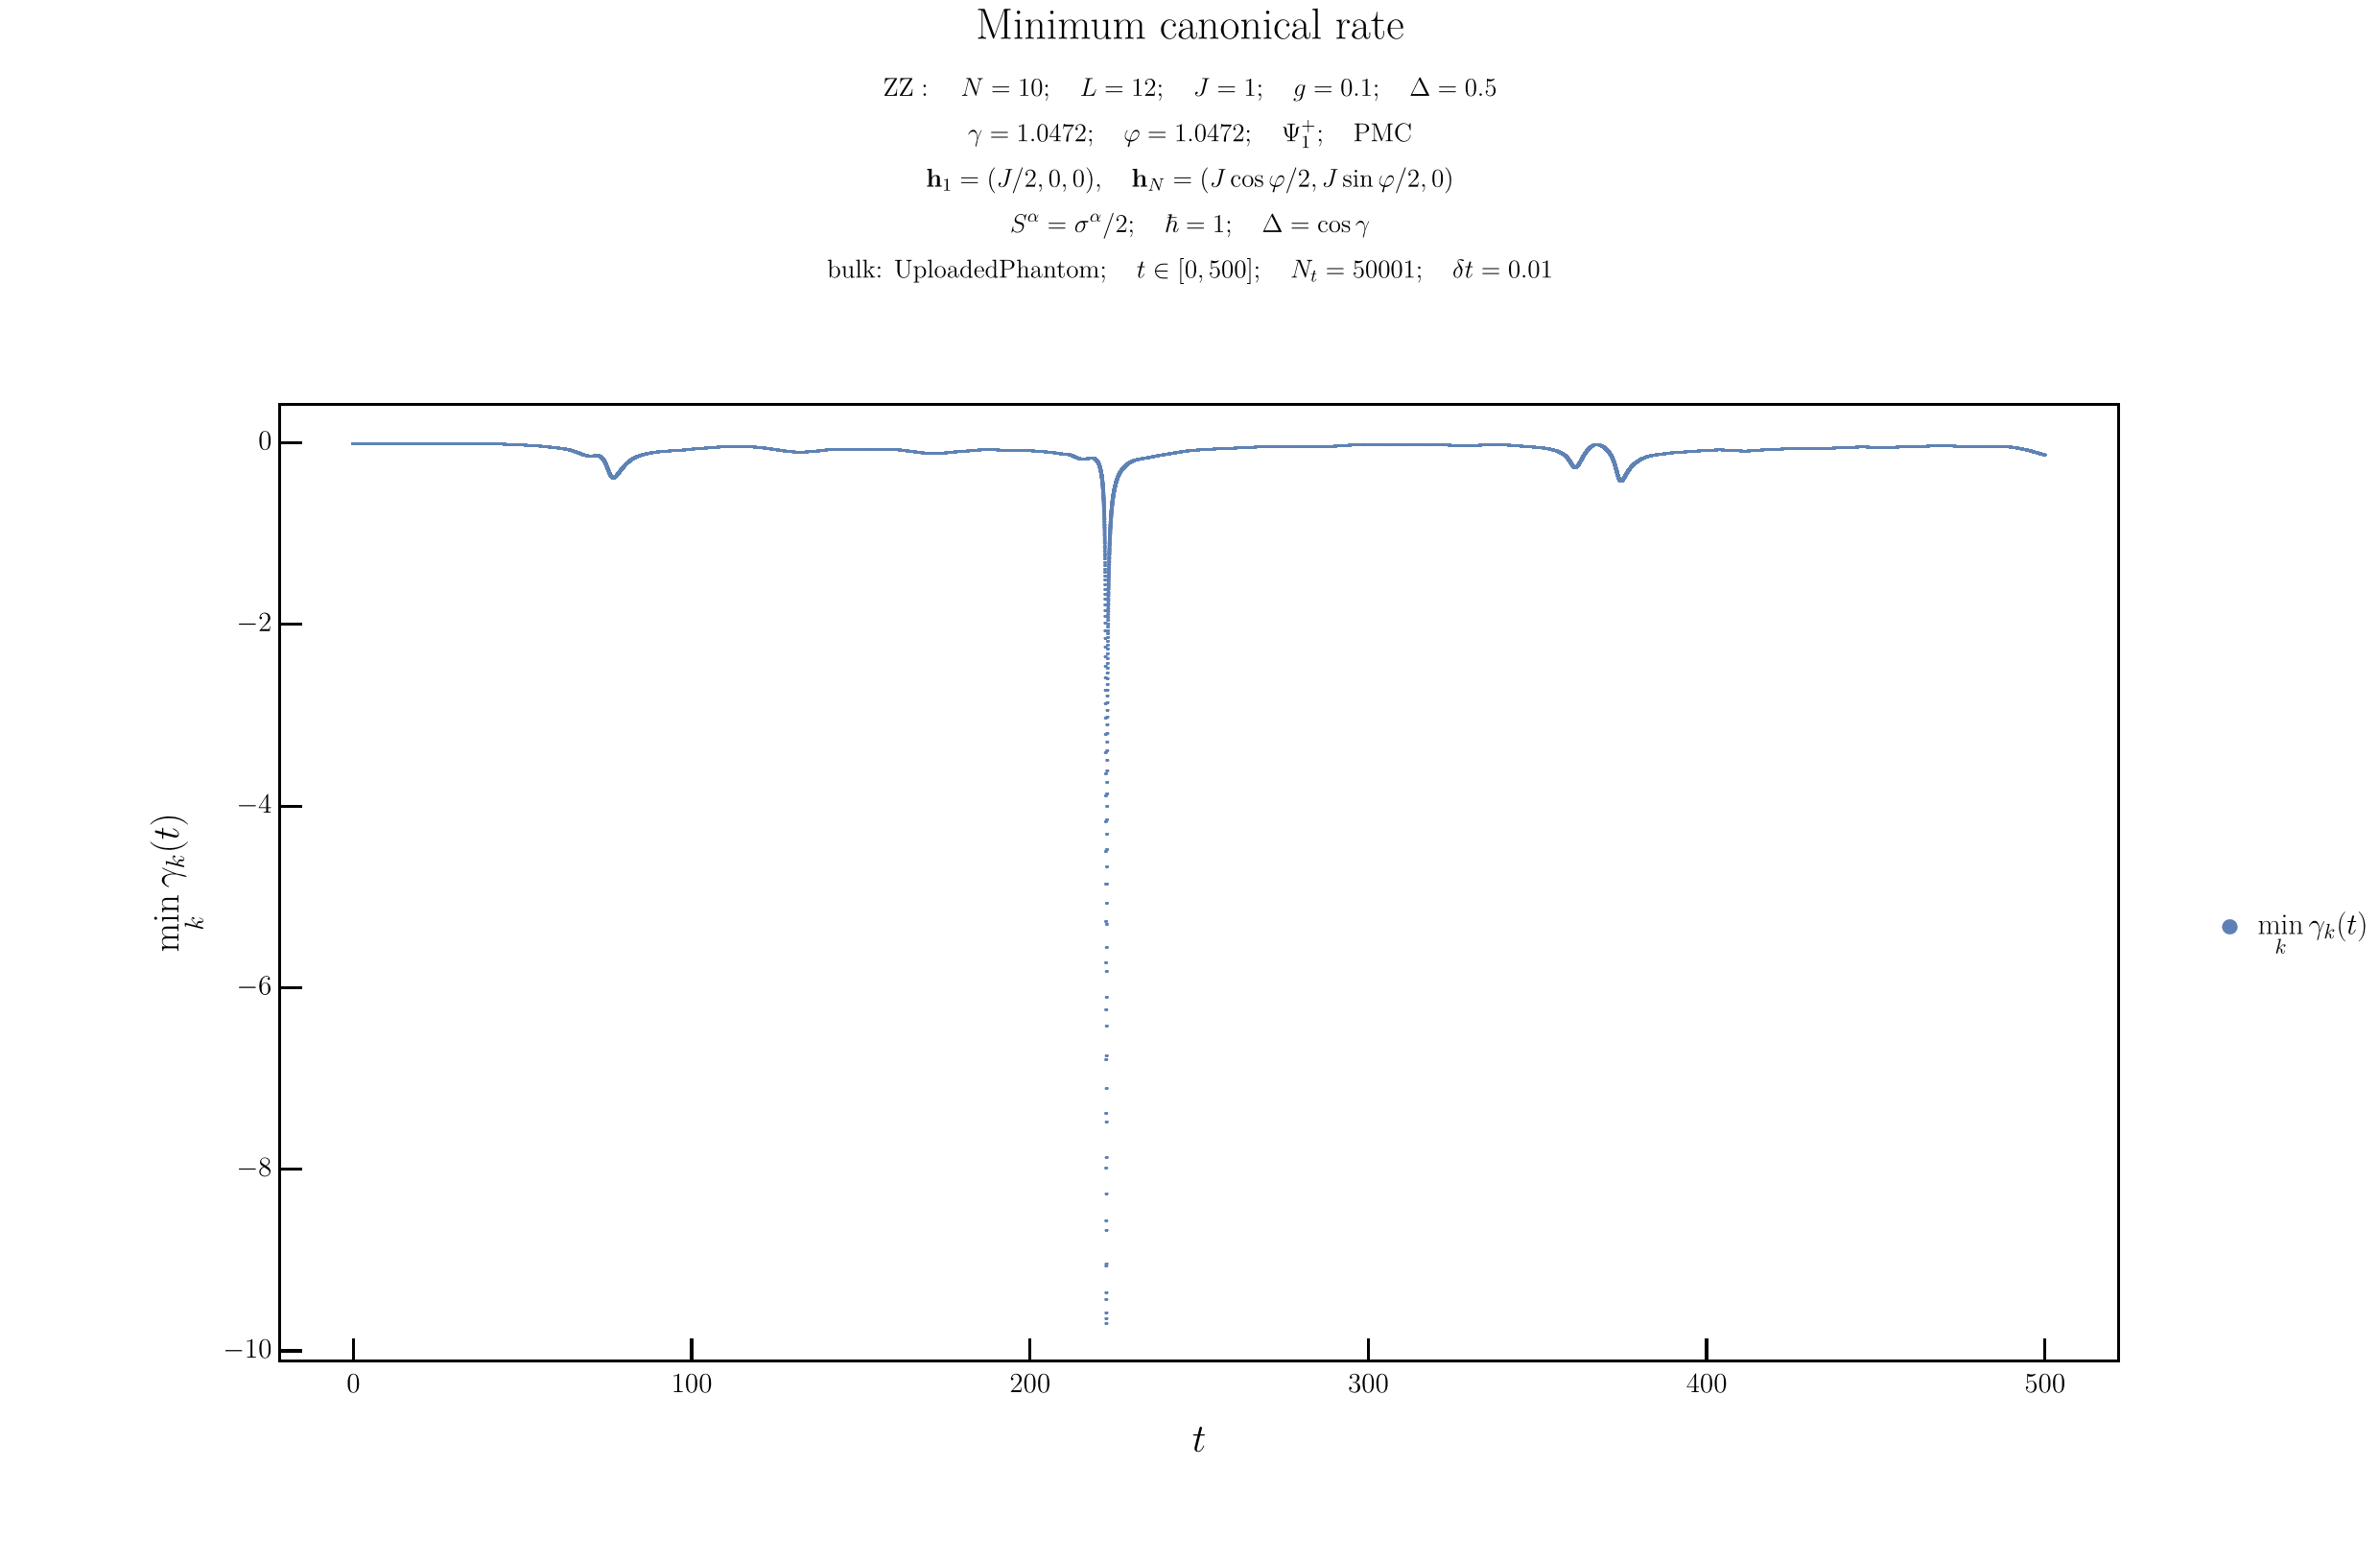
\includegraphics[width=\linewidth,height=0.36\textheight,keepaspectratio]{Phantom_ZZ_N10/Channel_MinimumRate.png}
\end{column}
\begin{column}{0.48\textwidth}
\centering
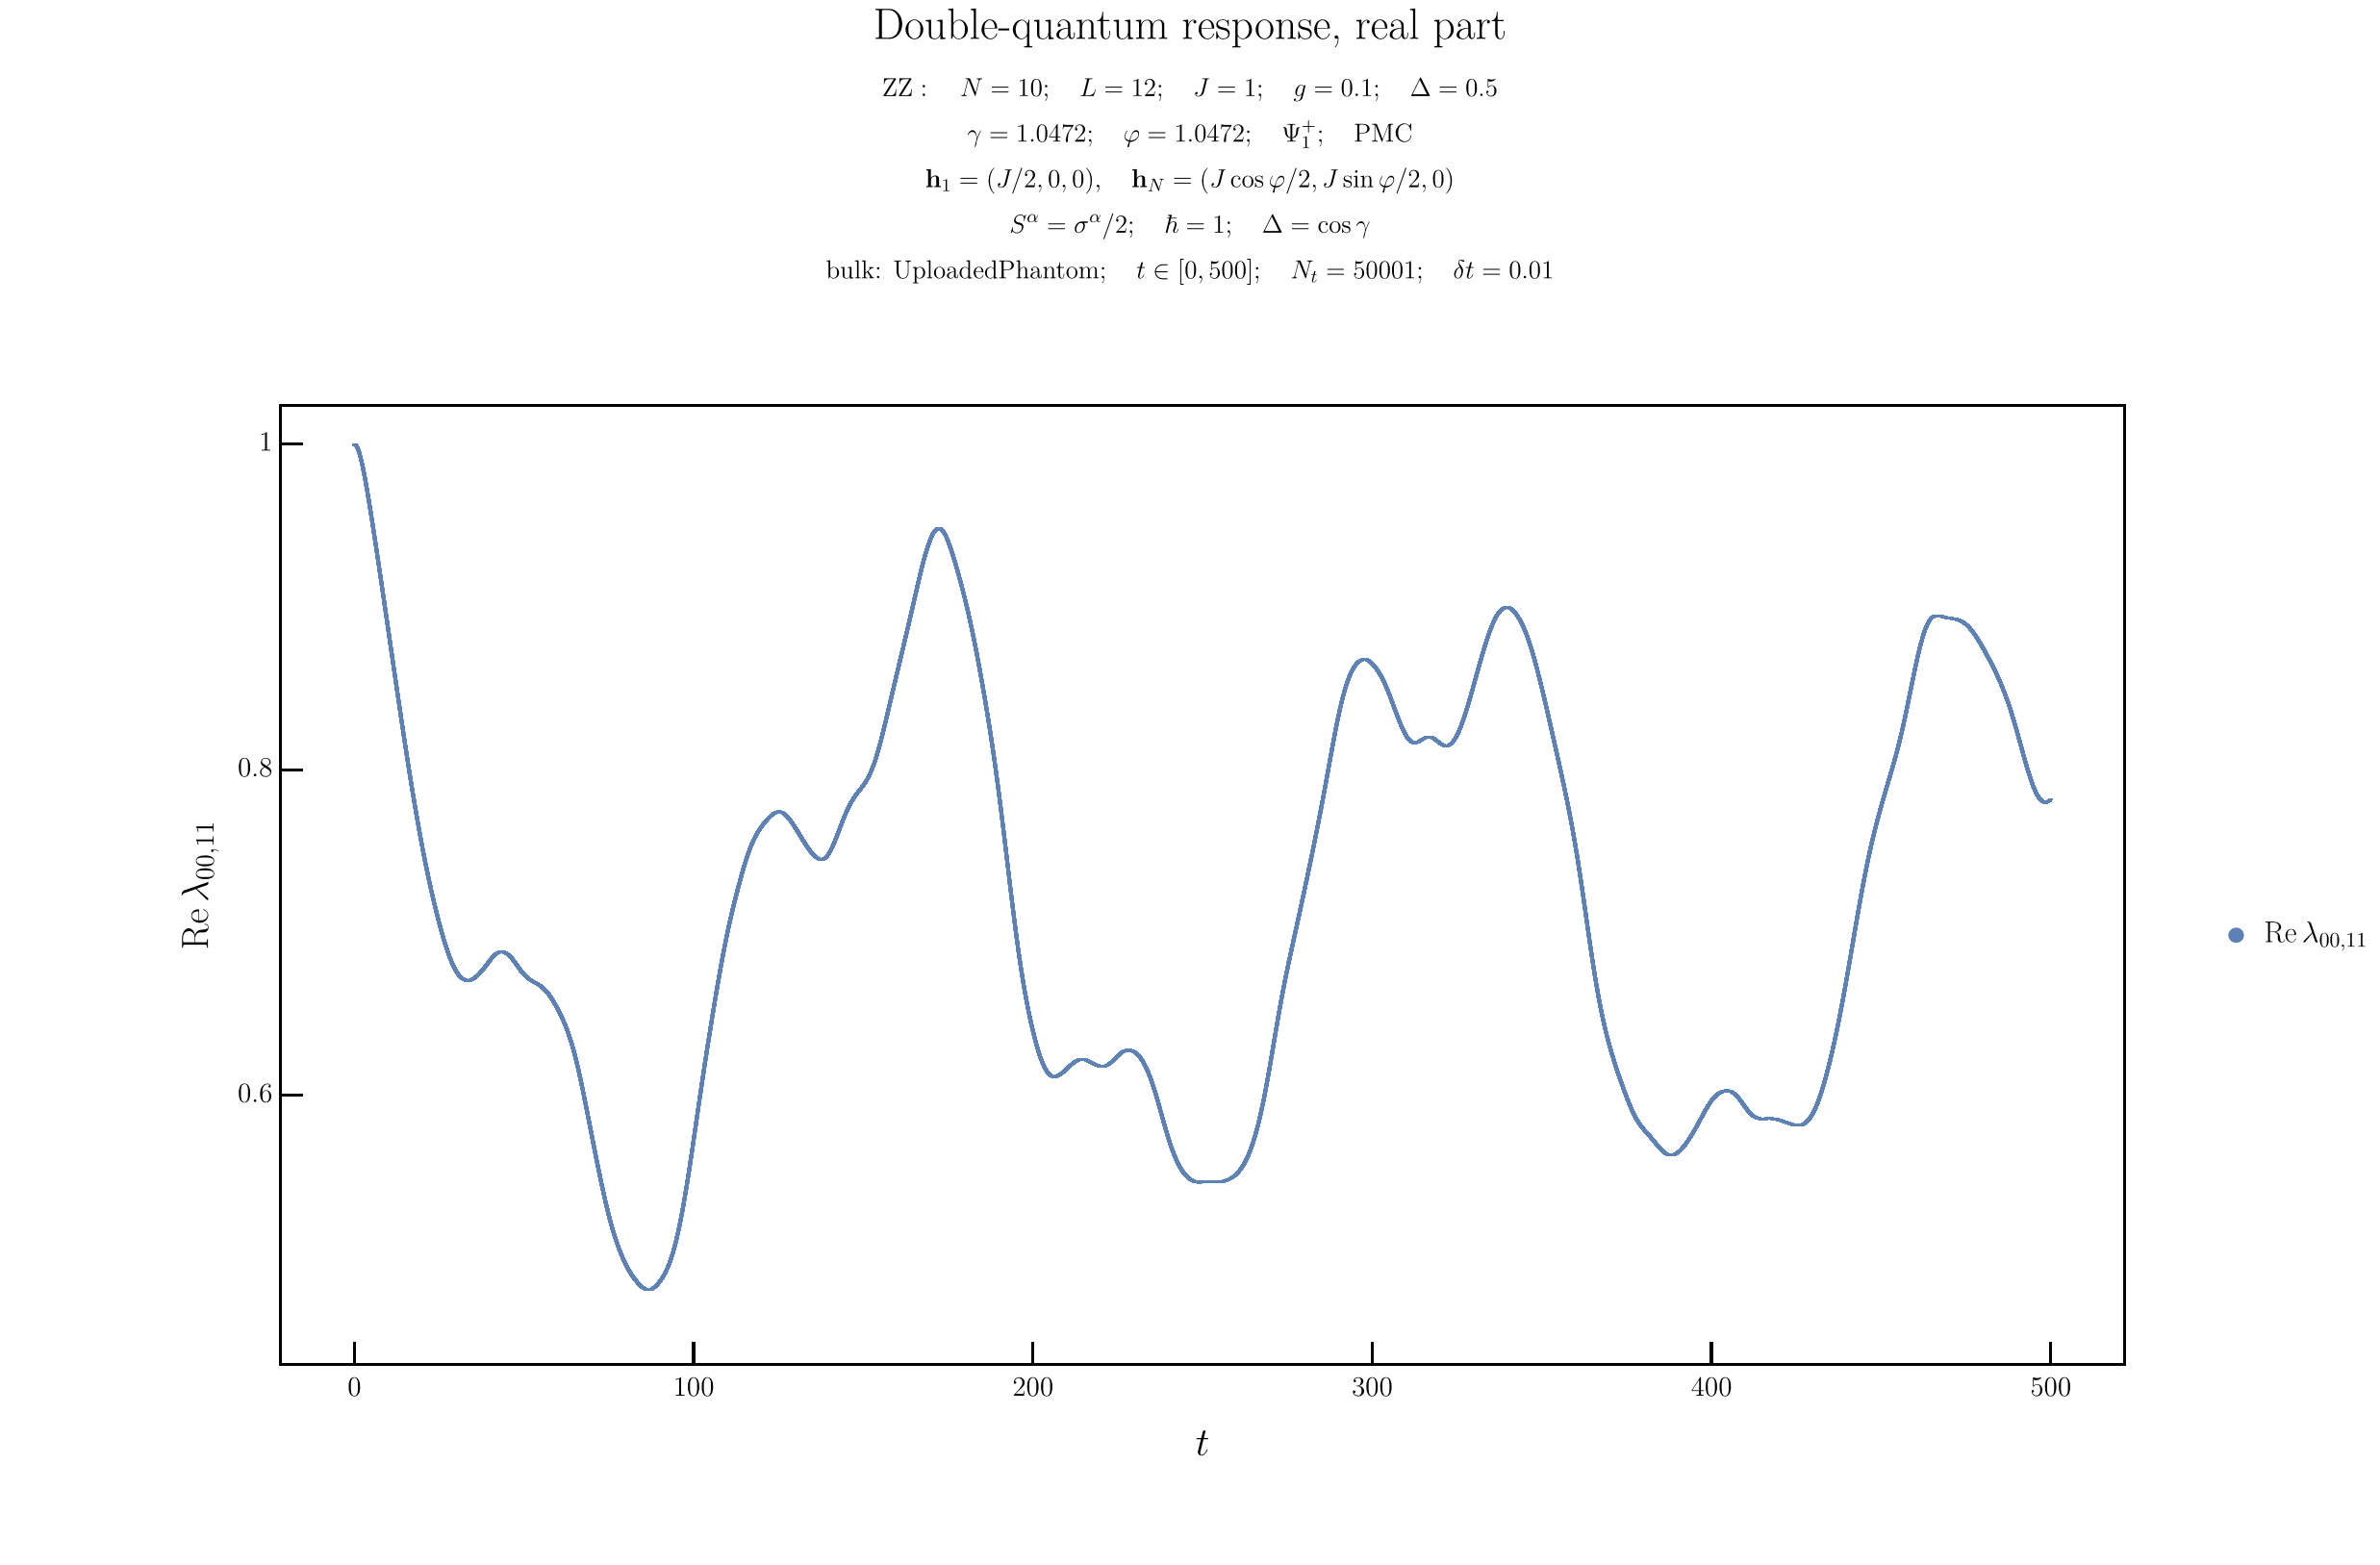
\includegraphics[width=\linewidth,height=0.36\textheight,keepaspectratio]{Phantom_ZZ_N10/Channel_DoubleQuantumReal.png}\\[3pt]
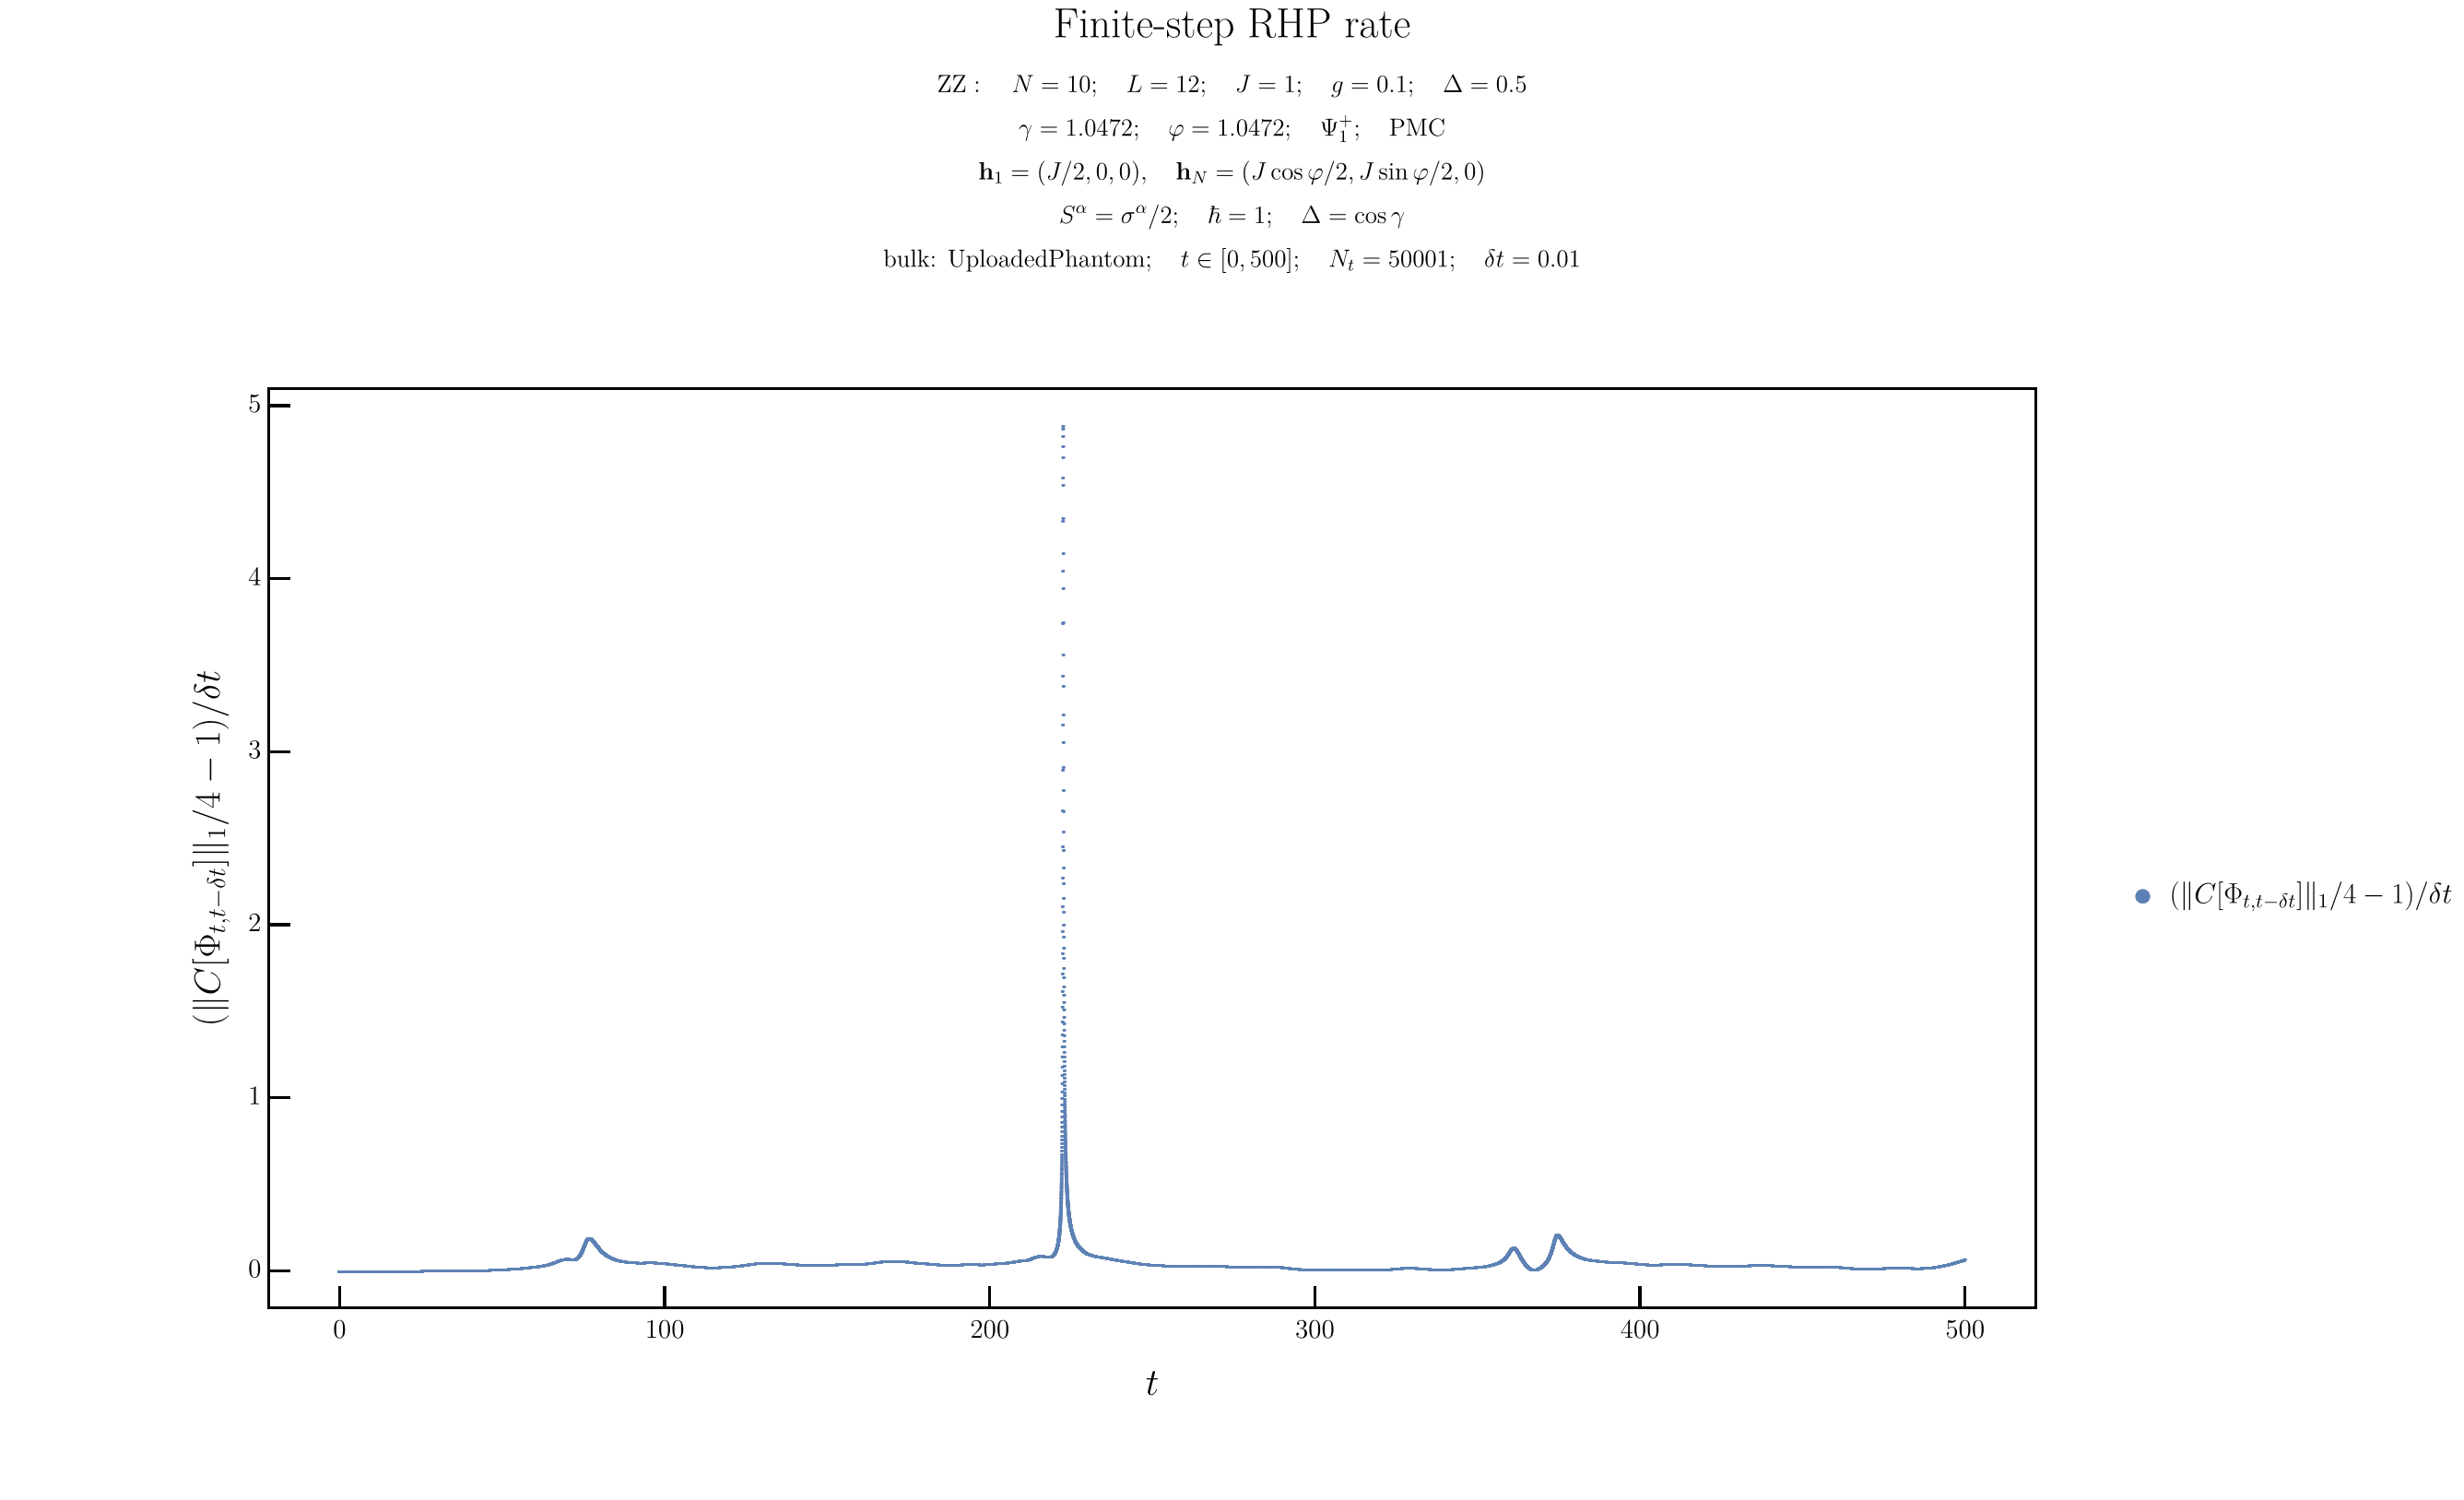
\includegraphics[width=\linewidth,height=0.36\textheight,keepaspectratio]{Phantom_ZZ_N10/Channel_RHPFiniteStepRate.png}
\end{column}
\end{columns}
\vspace{2pt}
\mutednote{Top: $\lVert[\St,\mathcal F]\rVert_{\max}\equiv\lVert[\St,\mathcal R]\rVert_{\max}$ and $\operatorname{Re}\Gamma_{00,11}$. Bottom: $\min_k\gamma_k=\gamma_1(t)$ and finite-step RHP rate $r_k=w_k/\delta t$.}
\end{frame}

% ==============================================================
\begin{frame}{Appendix 2d: Mixed longitudinal--transverse correlations}
\footnotesize
\begin{columns}[T,totalwidth=\textwidth]
\begin{column}{0.49\textwidth}
\centering
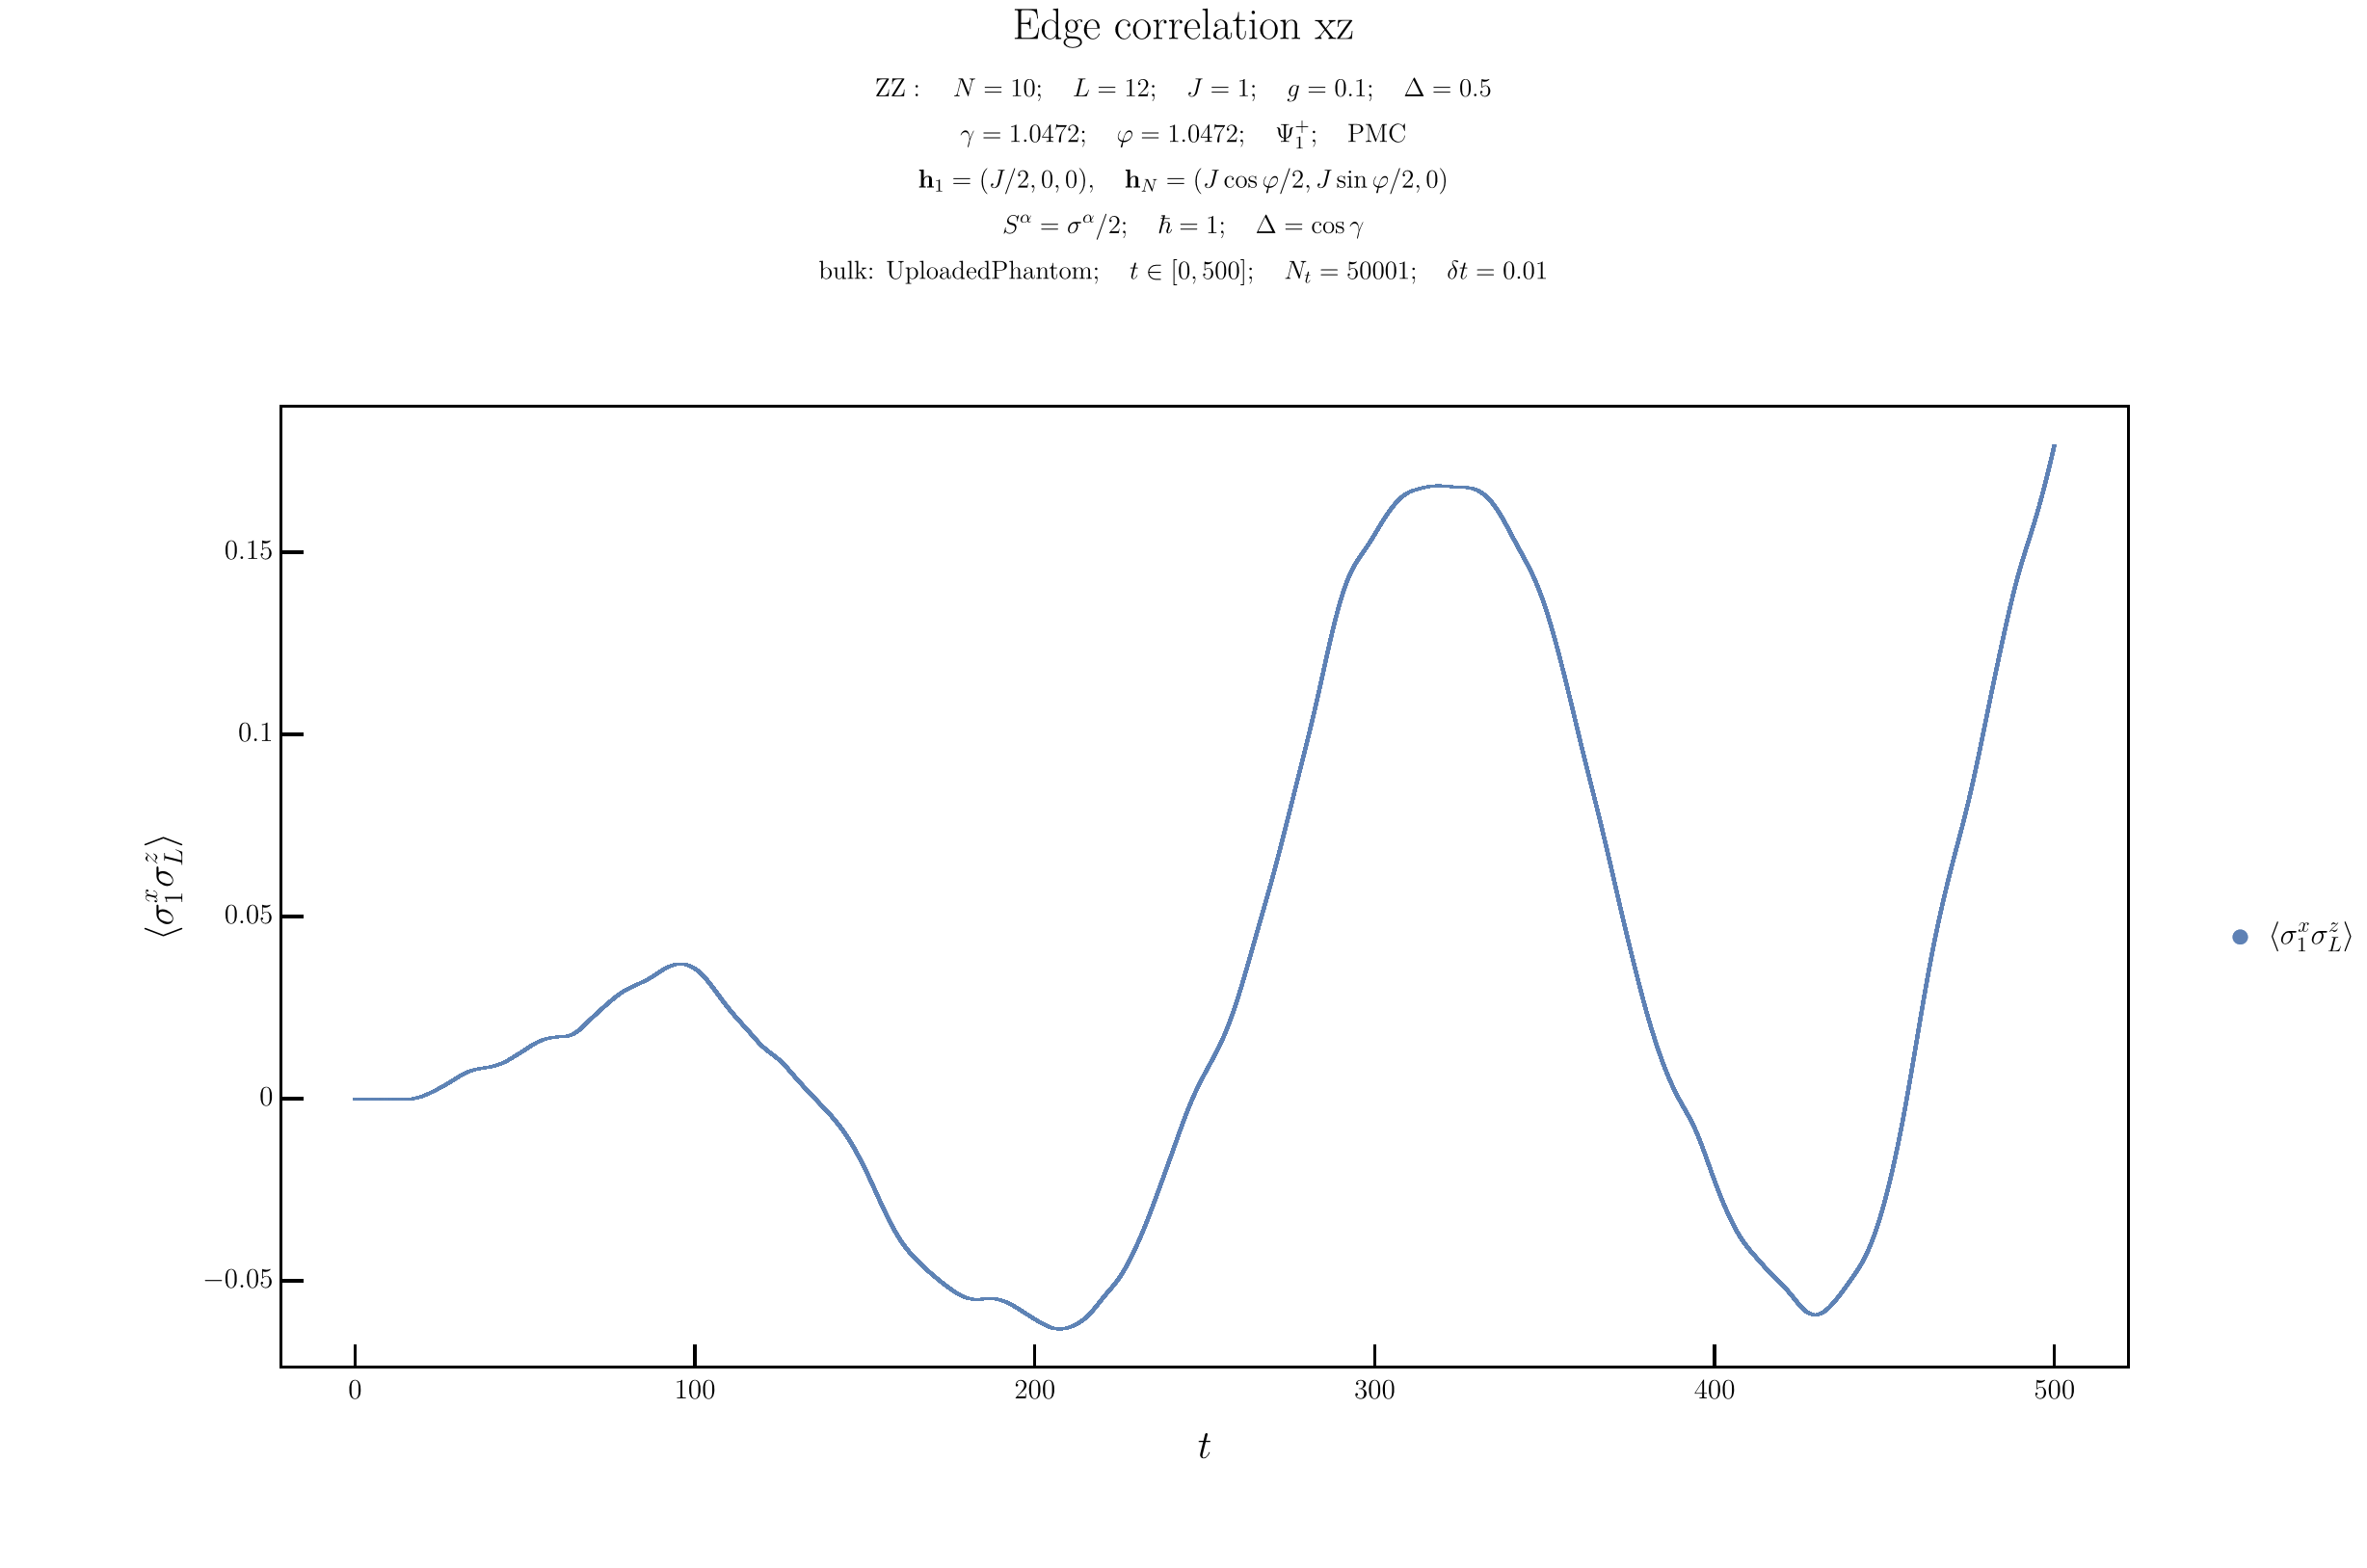
\includegraphics[width=\linewidth,height=0.52\textheight,keepaspectratio]{Phantom_ZZ_N10/State_CorrelationXZ.png}
\end{column}
\begin{column}{0.49\textwidth}
\centering
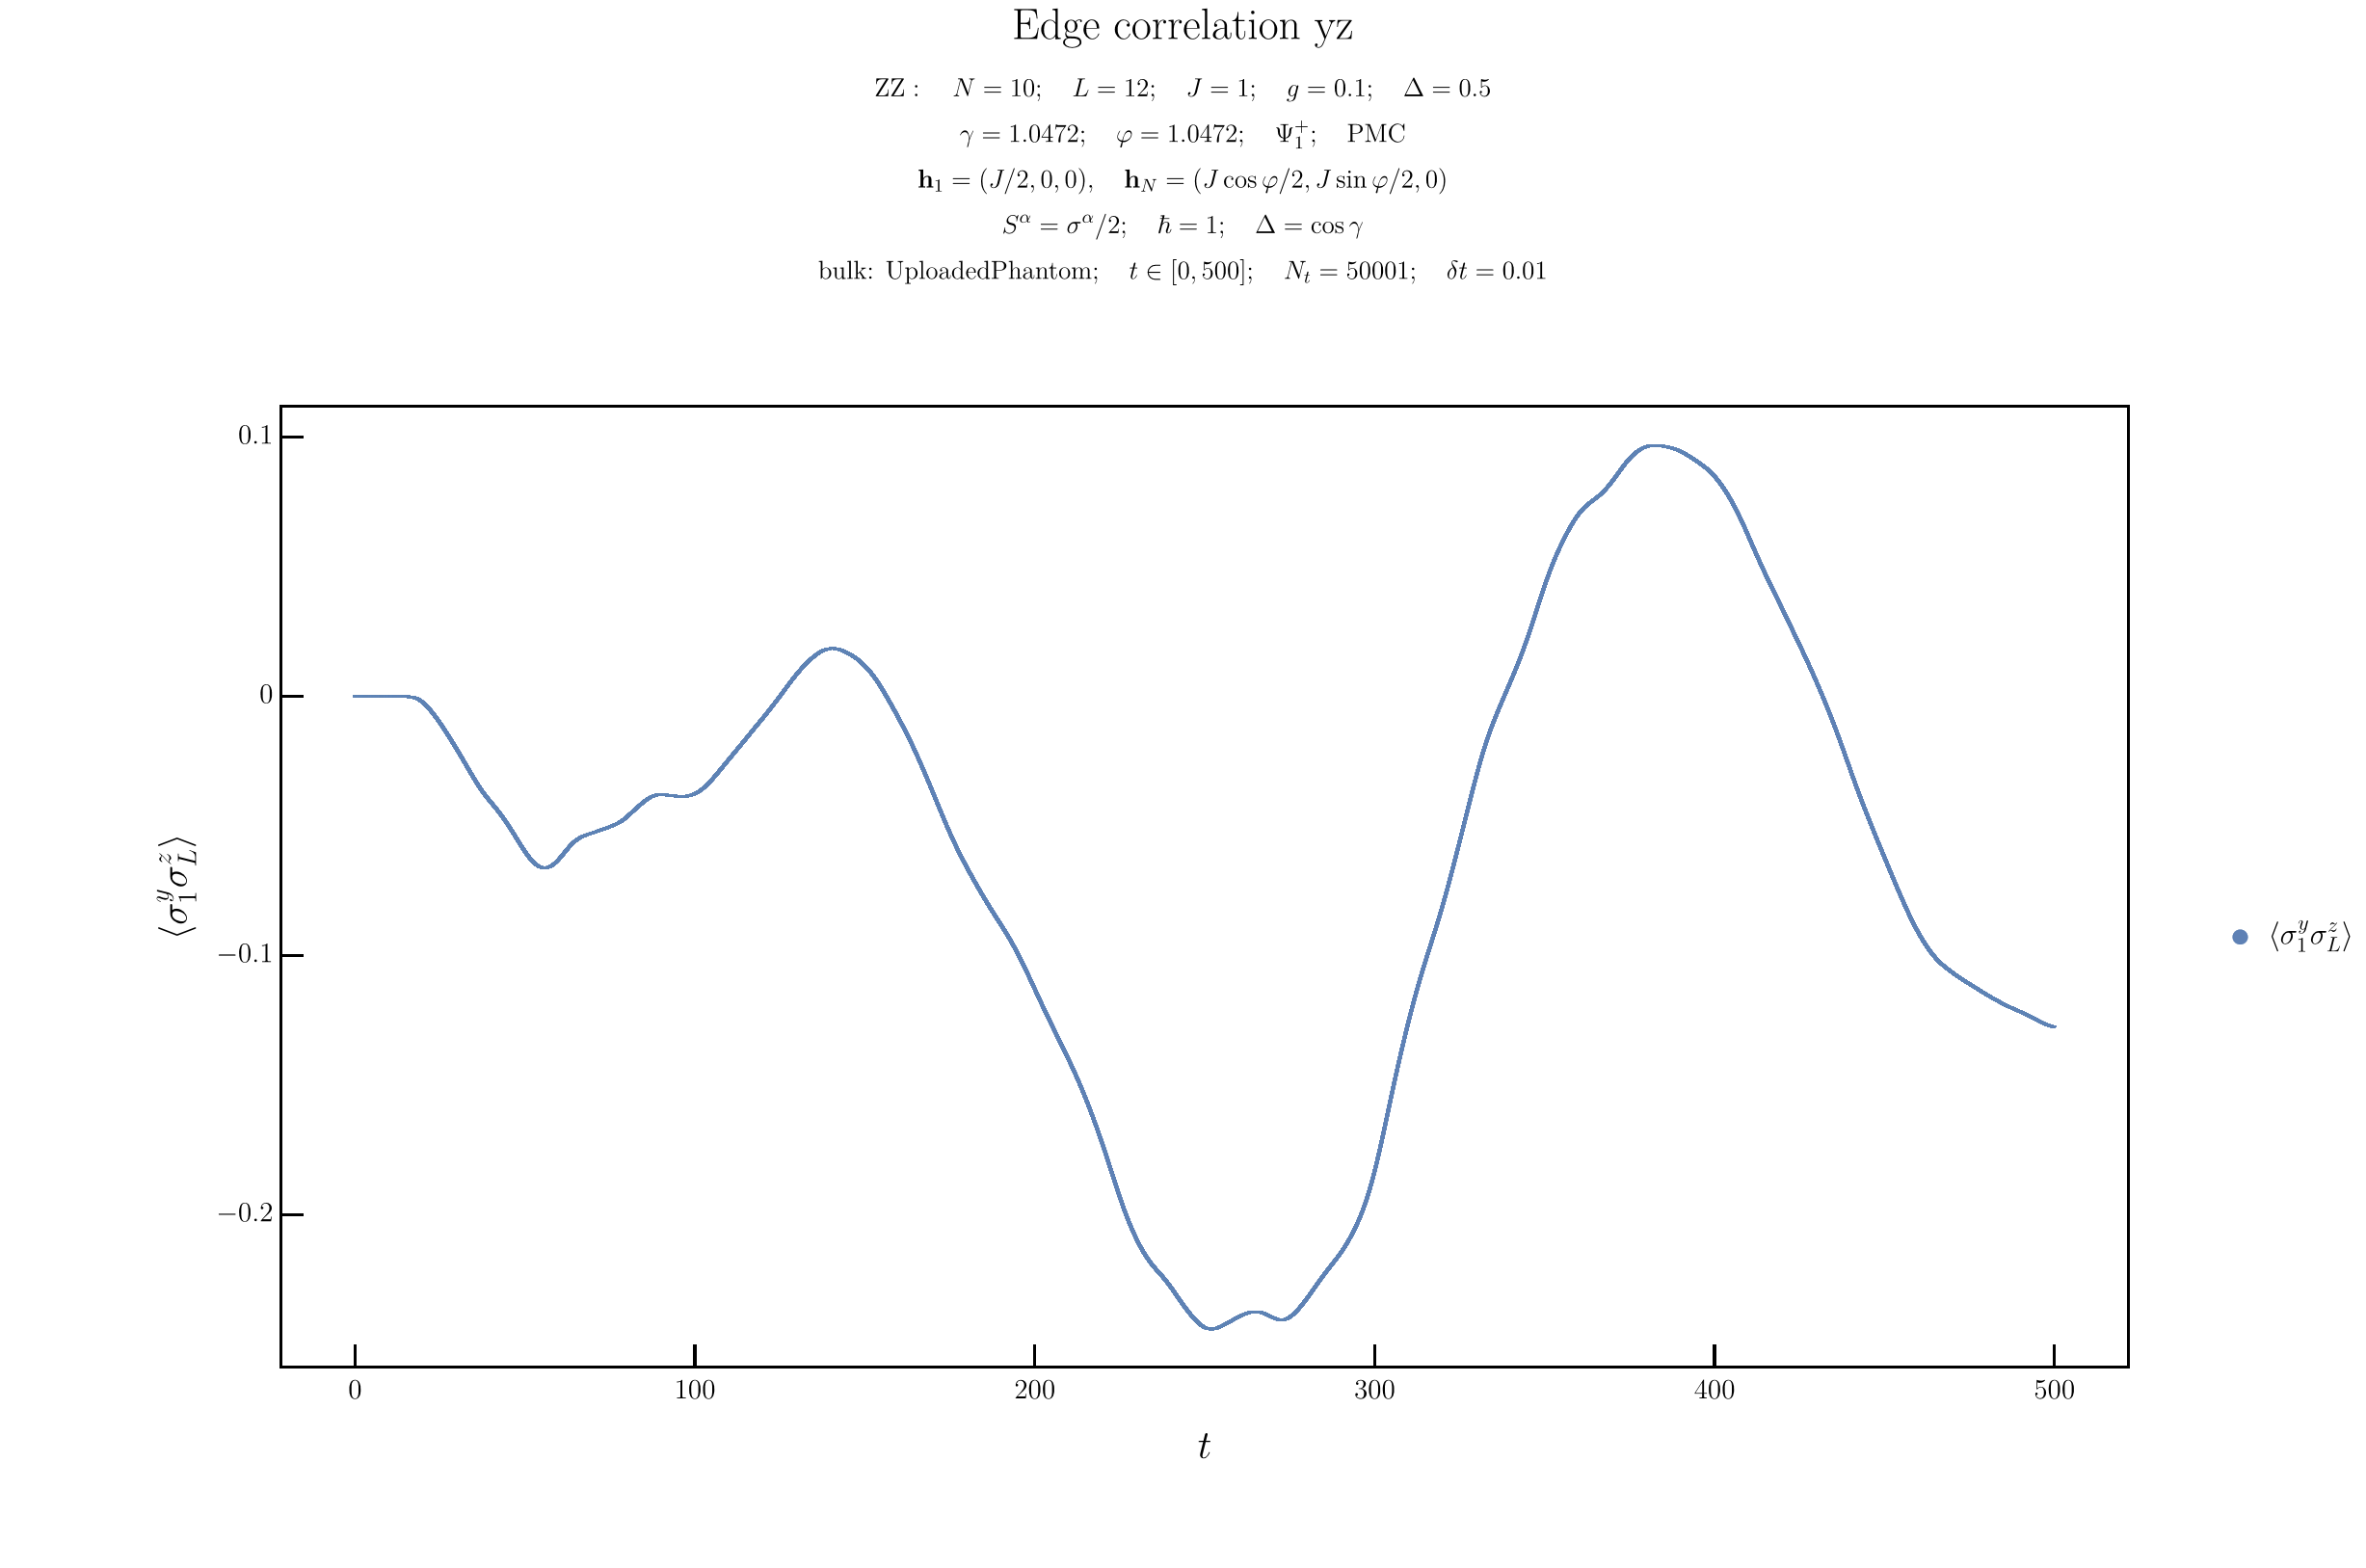
\includegraphics[width=\linewidth,height=0.52\textheight,keepaspectratio]{Phantom_ZZ_N10/State_CorrelationYZ.png}
\end{column}
\end{columns}
\[
\langle\sigma_A^x\sigma_B^z\rangle=\tfrac12\operatorname{Re}\bigl(\Gamma_{00,10}-\Gamma_{01,11}\bigr)=-\langle\sigma_A^z\sigma_B^x\rangle,\qquad
\langle\sigma_A^y\sigma_B^z\rangle=-\tfrac12\operatorname{Im}\bigl(\Gamma_{00,10}-\Gamma_{01,11}\bigr)=+\langle\sigma_A^z\sigma_B^y\rangle .
\]
\begin{itemize}\setlength\itemsep{2pt}
\item Both stay near $0$ until $t\approx 20$ (Lieb--Robinson light cone across $N=10$ bulk sites) and equal their connected counterparts because $\langle\sigma_{A,B}^z\rangle\equiv 0$.
\end{itemize}
\end{frame}

% ==============================================================
\begin{frame}{Appendix 3a: Derivation of $\dmat(t)=G^{\mathsf T}\eta(t)G$ (I)}
\small
\textbf{Step 1 --- Entrywise generator on $E_{ab}=\ket a\bra b$ (whenever $\Gamma_{ab}(t)\neq 0$):}
\[
\rho_{ab}(t)=\Gamma_{ab}(t)\,r_{ab}
\quad\Longrightarrow\quad
\dot\rho_{ab}(t)=\eta_{ab}(t)\,\rho_{ab}(t),\qquad
\eta_{ab}(t)=\frac{\dot\Gamma_{ab}(t)}{\Gamma_{ab}(t)}=-\kappa_{ab}(t)+i\omega_{ab}(t).
\]
\textbf{Step 2 --- Diagonal restriction of Hall's canonical GKS--Lindblad form \cite{Hall2014}:}
\[
\mathcal L_t(\rho)=-i[\Heff(t),\rho]+\sum_{\mu,\nu=1}^{3}\dmat_{\mu\nu}(t)\Bigl(F_\mu\rho F_\nu-\tfrac12\{F_\nu F_\mu,\rho\}\Bigr).
\]
\begin{itemize}\footnotesize\setlength\itemsep{3pt}
\item $\mathcal L_t$ commutes with $\operatorname{Ad}_{D_\theta}$ for every diagonal unitary $D_\theta=\diag(e^{i\theta_a})$, so by uniqueness $\Heff=\sum_a h_a P_a$ ($\sum_a h_a=0$) is diagonal and the $15\times 15$ decoherence matrix decouples between $\{F_\mu\}$ and $\{E_{ab}\}_{a\neq b}$.
\item Fixed populations, $\mathcal L_t(E_{bb})=0$, force all off-diagonal jump rates $E_{ab}$ to vanish, confining $\dmat(t)$ to $F_1=\tfrac12\sigma_A^z\otimes I$, $F_2=\tfrac12 I\otimes\sigma_B^z$, $F_3=\tfrac12\sigma_A^z\otimes\sigma_B^z$.
\end{itemize}
\end{frame}

% ==============================================================
\begin{frame}{Appendix 3b: Derivation of $\dmat(t)=G^{\mathsf T}\eta(t)G$ (II)}
\small
\textbf{Step 3 --- Eigenvalue matrix $G$ of $\{F_1,F_2,F_3\}$ on $\{\ket{00},\ket{01},\ket{10},\ket{11}\}$:}
\[
G=\frac12\begin{pmatrix}1&1&1\\1&-1&-1\\-1&1&-1\\-1&-1&1\end{pmatrix},\qquad
G^{\mathsf T}G=I_3,\qquad G^{\mathsf T}\mathbf1=0.
\]
\textbf{Step 4 --- Closed-form inversion ($12$ real parameters $\leftrightarrow$ $12$ real parameters):}
Evaluating $\mathcal L_t(E_{ab})=\eta_{ab}E_{ab}$ with Hermitian $\dmat=S+iA$ ($q_a=\tfrac12\mathbf g^{a\mathsf T}S\mathbf g^a$) yields
\[
\eta(t)=G\,\dmat(t)\,G^{\mathsf T}+(-ih-q)\mathbf1^{\mathsf T}+\mathbf1(ih-q)^{\mathsf T},
\]
so multiplying by $G^{\mathsf T}(\cdot)G$ annihilates the rank-$1$ $\mathbf1$ terms and summing $\operatorname{Im}\eta_{ab}$ isolates $h_a$:
\[
\boxed{\dmat(t)=G^{\mathsf T}\eta(t)\,G,\qquad
h_a(t)=-\frac14\sum_{b}\operatorname{Im}\eta_{ab}(t),\qquad
\Heff(t)=\sum_a h_a(t)\ket a\bra a .}
\]
\end{frame}

% ==============================================================
\begin{frame}{References}
\footnotesize
\nocite{Hall2014,Wootters1998}
\bibliographystyle{unsrtnat}
\bibliography{references}
\medskip
\begin{itemize}\footnotesize\setlength\itemsep{4pt}
\item H.-P.\ Breuer, E.-M.\ Laine, and J.\ Piilo, \emph{Measure for the Degree of Non-Markovian Behavior of Quantum Processes in Open Systems}, Phys.\ Rev.\ Lett.\ \textbf{103}, 210401 (2009).
\item \'A.\ Rivas, S.\ F.\ Huelga, and M.\ B.\ Plenio, \emph{Entanglement and Non-Markovianity of Quantum Evolutions}, Phys.\ Rev.\ Lett.\ \textbf{105}, 050403 (2010).
\item H.\ T.\ Quan, Z.\ Song, X.\ F.\ Liu, P.\ Zanardi, and C.\ P.\ Sun, \emph{Decay of Loschmidt Echo Enhanced by Quantum Criticality}, Phys.\ Rev.\ Lett.\ \textbf{96}, 140604 (2006).
\end{itemize}
\end{frame}

\end{document}
